\documentclass[a4paper,oneside,openright]{book}
\usepackage[a4paper,margin=1in]{geometry}
\usepackage[utf8]{inputenc}
\usepackage[T1]{fontenc}
\usepackage{graphicx}
\usepackage[bookmarks=true,colorlinks=true]{hyperref}
\usepackage{framed} % box frames
\usepackage{enumitem} % resume list numbering
\usepackage[english]{babel} % bibliography
\usepackage{lmodern,textcomp} % font
\usepackage[table]{xcolor}
\usepackage{tabularx}
\usepackage{amsfonts}
\usepackage{pifont}
\usepackage{url}
\usepackage{hyperref}
\usepackage{listings}
\usepackage[numbers]{natbib}
\bibliographystyle{plainnat}
\usepackage{bibentry}
\nobibliography*
\usepackage{todonotes}

% redefine autoref macros
\renewcommand*{\chapterautorefname}{Chapter}
\renewcommand*{\sectionautorefname}{Section}
\renewcommand*{\subsectionautorefname}{Section}

% checkmark
\newcommand{\cmark}{\ding{51}}%
\newcommand{\xmark}{\ding{55}}%

\title{Representing Activites associated with Personal Data and Consent using Semantic Web for GDPR Compliance}
\author{Harshvardhan J. Pandit}
\date{Ph.D. thesis\\draft\\\today\\
    \vspace{5mm}
    Chapters to be reviewed:\\
    \autoref{chapter:sota} SotA \\
    \autoref{chapter:information} Information Required for GDPR Compliance \\
    \vspace{5mm}
    Chapters being written:\\
    \autoref{chapter:vocabularies} Representing Information using Ontologies
    }

\begin{document}

\maketitle
% \setcounter{tocdepth}{3}
\tableofcontents

% \chapter{Introduction}
\label{chapter:introduction}

\section{Background \& Motivation}\label{sec:intro:background}
% privacy laws across the world
% disconnect with technological progress
To date, 132 of the 206 states listed by the United Nations (UN) have a privacy law which regulates the usage of personal data \cite{greenleaf_global_2019-1}.
However, their intended application suffers from a disconnect with the rapid progress in technology. In particular, the use of internet as a medium for data exchange and its pervasiveness and connectivity to individuals via devices such as the smartphone has led to industrial data harvesting at large scales \cite{christl_networks_2016}. 
To counter this problem, lawmakers in the European Union (EU) passed the General Data Protection Regulation (GDPR) \cite{Regulation_GDPR} in 2016 with the aim of providing individuals with the right to information and control over use of their personal data, and to simplify requirements for organisations through a unified regulation across the EU.

The GDPR has received a large amount of attention due to its prospective fines which can potentially be up to 4\% of an organisation's annual turnover or €20 million - whichever is greater. 
As of February 2020, there have been over 215 publicly known instances of fines associated with the GDPR \cite{GDPR_fines_tracker}, the largest of which was the €50 million fine to internet giant Google \cite{CNIL_GOOGLE_2019}.
Being a regulation and replacing the Data Protection Directive (DPD) \cite{directive_DPD}, GDPR provides a uniform set of compliance requirements across the EU, and is the basis of national privacy laws implemented in its member states \cite{mccullagh_national_2019}.
Furthermore, GDPR has influenced other privacy laws, such as the California Consumer Protection Act (CCPA) \cite{CCPA}, thereby further expanding similarities in compliance requirements across the globe.

The most visible change of the GDPR for most individuals is the ubiquitous `consent dialogue' on websites that requests `consent' - one of the legal basis for processing of personal data in GDPR.
Despite being a legal requirement, consent dialogues have been accused of being non-transparent and subverting the spirit of the GDPR \cite{machuletz_multiple_2019,utz_informed_2019}.
The issue of consent itself has received significant interest in development and utilisation of technological solutions for compliance due to the right to withdraw consent provided by the GDPR which enables an individual to revoke their previously given consent and requires processing of personal data based on it to be halted.
Opinions published by legal experts and bodies, in absence of case law on this issue, have expressed the need for greater transparency regarding activities associated with use of consent \cite{opinion_AG_2019}.

% information associated with gdpr compliance
Compared to other privacy laws, including its predecessor DPD, GDPR provides significantly stricter and detailed requirements for processing of personal data and requires organisations to explicitly document information in relation to its obligations in order to be compliant.
This information consists of identification of GDPR clauses applicable to the practices of an organisation and the steps taken to fulfil requirements and obligations for compliance.
From a technical or information management point of view, GDPR specifies interactions between entities in a clear manner. An example of this is an organisation using consent as the legal basis being required to provide information about processing activities to the data subject. Furthermore, this information is required to be maintained, evaluated, and documented to demonstrate compliance upon request by authorities. At the same time, this information is also associated with other stakeholders - such as through privacy policies, user agreements, terms and conditions, or even data processing agreements. This makes it clear that information associated with GDPR compliance is also used in other applications and involves multiple stakeholders.

As GDPR is a data protection law, its compliance is concerned primarily with processing of personal data, its legality, and associated operations within an organisation. 
This includes processing in both tenses - past as well as future - where an organisation is obligated to first determine and ensure its requirements and activities involving processing of personal data are valid as per the GDPR, and to then maintain a record of such activities as the processing takes place.
These are defined\footnote{Defined in EU terminology database (IATE) \url{https://iate.europa.eu/entry/result/787324/en}} within the legal domain by the terms `ex-ante' to specify compliance assessment before activity takes place (preventative) and `ex-post' to specify compliance assessment after the activity has taken place (corroborative).

While the GDPR does not explicitly mention a `phase' of compliance, its use enables associating the information to the planning and processing operations carried out within an organisation. The planning of processing operations also involves investigation of whether the intended operations will be compliant to the legal obligations, and the required corrections to ensure they continue to be so. The processing operations carried out also need to be inspected to ensure they met the requirements set forth in the planning stage and that the processing itself was legally compliant.

The combination of new requirements and significant fines has provided an incentive to utilise technology in meeting the obligations and requirements stipulated by GDPR towards its compliance.
Existing efforts, such as the International Organization for Standardization (ISO), have addressed this change by updating standards to meet increased requirements with global privacy laws.
In the context of GDPR, ISO/IEC 27001\footnote{\url{https://www.iso.org/standard/54534.html}} defines requirements for an information security management system, and its extension ISO/IEC 27701\footnote{\url{https://www.iso.org/standard/71670.html}} defines a privacy information management system, which together provide a framework for managing privacy risks associated with personal data processing.
Adherence to such standards provides a commonality in the information management practices of an organisation, and assists in the compliance process by providing a structured interpretation and demonstration of practices based on the standardised specifications.

% challenges in developing technological solutions
Technological development of solutions for legal compliance face two problems in general - the first being algorithmic interpretation of requirements associated with legal compliance. This is difficult as the text used in a legal document such as GDPR does not readily lead to algorithmic compliance due to ambiguity and uncertainty in its legal interpretation - especially in domain specific use-cases.
In addition, because GDPR has been enforced for a comparatively short period - the interpretation of its clauses as requirements for compliance relies on clarification through legal opinions and decisions by supervisory authorities and courts.
The second problem is that regardless of how technology is used in the compliance process, formal investigations of legal compliance require information to be documented and associated with the specifics of the law they intend to comply with - in this case the articles and clauses of GDPR.
Traditionally, this is carried out through creation of documentation by legal experts, lawyers, and legal departments.
Therefore, technological solutions addressing GDPR compliance must also provide information documentation in addition to assessment of compliance. 

% problem with existing text based approaches
Incorporating legal compliance into organisational requirements has led to several approaches such as: use of symbolic (mathematical) logic, knowledge representation of legal text as logical rules, deontic rights specifying rights and obligations, defeasible logic based on exceptions, first order temporal logic, access control, markup based representations, and goal modelling of obligations \cite{otto_addressing_2007}.
While there has been significant work in the use of technology to adopt these approaches towards addressing and evaluating compliance in the last decade \cite{sadiq_modeling_2007,otto_addressing_2007,gordon_rules_2009,fellmann_state---art_2014,benyoucef_information_2015,elgammal_formalizing_2016,kirrane_access_2016}, the issue of associating information with legal documents has received relatively less attention.
Where contemporary methods are sufficient to meet legal requirements, their use of text-based document formats prevents effective technological solutions that can be scaled, automated, or utilised in an information management system. To enable such approaches, information associated with compliance must be represented using machine-readable formats that enable the use of querying to retrieve information as well as validation methods to ensure its correctness. Furthermore, the need to share information between stakeholders defined within the GDPR provides motivation towards developing interoperability in information and solutions - which also provides transparency in the compliance process. By using open and interoperable standards, the commonality in representation and interpretation of information benefits stakeholders and reduces costs associated with innovation regarding information management and regulatory compliance.

% linked data principles and ELI, Akoma Ntoso
Governmental agencies across the globe have addressed the issue of information interoperability by adopting the principles of Linked Data \cite{bizer_linked_2011} and have produced interoperable standards \cite{palmirani_akoma_2018,european_union_eli_2015,van_opijnen_european_2011} to facilitate use of information in technological solutions.
These standards implement principles of the Semantic Web \cite{semantic-web} by utilising the Resource Description Framework (RDF) \cite{RDF} to specify information in an interoperable, extensible, and machine-readable manner.
This has paved the way for development of technologies that address challenges associated with legal compliance through greater use of automation and operations at large scales.
Consequently, the use of Linked Data and Semantic Web within the legal domain has resulted in the development of ontologies for organising and structuring information, reasoning and problem solving, semantic indexing and search, semantic integration and interoperability, and understanding the domain \cite{rodrigues_legal_2019}.
Semantic Web is also being used to address the challenges associated with GDPR compliance through commercial\footnote{Example: Top Quadrant's Semantic Data Governance for GDPR Compliance \url{https://www.topquadrant.com/gdpr-compliance/}} solutions as well as large-scale European research projects such as SPECIAL \cite{SPECIAL}, MIREL \cite{MIREL}, DAPRECO \cite{DAPRECO}, BPR4GDPR \cite{BPR4GDPR}, and RestAssured \cite{RestAssured}.
The technological solutions developed within these utilise ontologies to represent the information required for compliance and a corresponding approach that expresses and evaluates obligations to assess compliance.

%%% link between GDPR compliance and research question???
The work presented in this thesis also utilises the Semantic Web to address GDPR compliance. It focuses on the representation of activities associated with processing of personal data and consent as a subset of information relevant to the investigation of GDPR compliance. These activities correspond to how organisations plan their processing of personal data and execute or implement them, and are therefore relevant to the planning and management of operations within organisations.
This includes activities associated with acquiring consent owing to the role of consent as a legal basis and the assertion that consent itself is also personal data.
The novelty of this work lies in the application of linked data principles to associate information with GDPR and the advantages this provides in utilising semantic web technologies to represent, query, and validate information relevant for compliance.

The role of semantic web in this is towards representing information relevant for GDPR compliance that can be associated with the text of GDPR following Linked Data Principles.
This involves use of existing standards of RDF \cite{RDF} and Web Ontology Language (OWL2) \cite{OWL} to represent information as ontologies, SPARQL \cite{SPARQL} for querying information, and Shapes Constraint Language (SHACL) \cite{SHACL} to validate information.
The use of semantic web standards and technologies enables the information to be persisted in a machine-readable, interoperable, and queryable form - and thus readily lends itself to automation using technological solutions in the areas of legal compliance and its documentation.

% The work presented in this thesis and representing its contributions is presented with a comparison to approaches identifed and analysed within the state of the art to demonstrate its novelty.

% Research Scope 
In terms of scope, the work presented in this thesis addresses only the representation and management of information associated with GDPR compliance, and is not intended to provide an authoritative assessment of compliance as only supervisory authorities and courts have legal authority in this matter.
In the same vein, the research presented in this thesis is also not intended to replace professional opinions such as that offered by lawyers and legal experts.
Instead, the intention of the work is to demonstrate the applicability and feasibility of using technology as a tool to assist with the compliance process.

\section{Research Question}\label{sec:intro:RQ}
% The aim of the thesis is to enable representation of information associated with ex-ante and ex-post activities involving processing of personal data and consent by using semantic web technologies for GDPR compliance.
The research question investigated in this thesis is:
\begin{framed}
\small{Research Question}
\begin{quote}
\textbf{To what extent can information regarding activities associated with processing of personal data and consent be represented using Semantic Web technologies for GDPR compliance?}
\end{quote}
\end{framed}

\subsection{Definitions}\label{sec:intro:definitions}
The following definitions are used in the context of the research question outlined above and this thesis:
\begin{itemize}
    \item \textit{information regarding activities}: information about how processes, services, tasks, or other similar concepts are planned, executed or carried out, along with the resulting outcomes and the artefacts used or required;
    \item \textit{activities associated with processing of personal data}: information about how personal data will be or has been obtained (its source), its usage - including storage, sharing, analysis, or other forms of processing;
    \item \textit{activities associated with consent}: information about how consent will be or has been obtained, its usage as a legal basis, the information represented by consent, and its planned or recorded withdrawal;
    \item \textit{querying}: retrieving information using a structured representation based on the underlying representation of information;
    \item \textit{validation}: assessment of information to meet a constraint or requirement;
    \item \textit{associate or link information with GDPR}: to establish an association or link between information and clauses or concepts of the text of GDPR;
    \item \textit{subset of GDPR}: a subset of the clauses defined in the text of the GDPR;
    \item \textit{ex-ante compliance}: compliance regarding processing before it has taken place, i.e. \textit{A-priori};
    \item \textit{ex-post compliance}: compliance regarding processing after it has taken place, i.e. \textit{A-posteriori};
    \item \textit{compliance questions}: questions that retrieve information relevant for determination of compliance.
\end{itemize}

\subsection{Research Objectives}\label{sec:intro:RO}
The research question represents a broad investigation which is difficult to address as a whole. Therefore, it is reconstructed as multiple `sub-research questions' which are smaller in scope and provide specific aims in the form of research objectives.

% RO1
The GDPR is a legal document structured into 173 Recitals, 99 Articles, and 21 Citations. Of these, not all clauses are relevant to activities associated with personal data and consent. Therefore, the first research sub-question concerns investigation and identification of the sub-set of GDPR regarding activities associated with personal data and consent, along with information on the ex-ante and ex-post aspects of such activities towards compliance. This provides the first objective as:
\begin{framed}
$RO1$: Identify the subset of GDPR relevant for activities associated with processing of personal data and consent regarding compliance.
\end{framed}

% RO2
Following identification of the relevant sub-set of GDPR, information required to represent activities needs to be identified through `compliance questions' representing an investigation process to identify the actors, entities, and relationships relevant for GDPR compliance. This provides the second objective as:
\begin{framed}
$RO2$: Identify information required to represent activities associated with processing of personal data and consent in investigation of GDPR compliance.
\end{framed}

% RO3
The identified information is then represented as semantic web ontologies consisting of concepts and relationships. This representation acts as the information model upon which questions or queries can be executed to retrieve information for determining compliance. The formalisation of information as an ontology provides a controlled vocabulary for validation of information to determine its sufficiency and correctness before determining compliance. 

% Rather than assimilating all information within a singular ontology, good practice dictates creation of modular ontologies specific to a particular task of domain. The information requirements can thus be divided into three distinct areas, each of which correspond to a specific topic or context, and lead towards the creation of an ontology within it. The first sub-objective concerns creating an ontology to associate information with the concepts and clauses within the text of the GDPR. The second objective utilises this ontology to represent activities associated with processing of personal data and consent. The third objective provides additional information regarding consent as required to determine its compliance. The distinction between the second and third objectives is based on the requirement of information other than that associated with activities in the determination of compliance for consent. 

Instead of representing all required information in a single large ontology, modular ontologies provide better reuse and are easier to engineer \cite{suarez-figueroa_neon_2012}.
A modular ontology is limited in scope towards representing a specific information category, and therefore is more consistent in its representation of concepts, and is easier to evaluate as compared to a larger ontology in which different concepts may have differing semantic connotations.
Modular ontologies also provide better motivation for reuse though selective choosing of concepts in a module without dependency of concepts in other modules.

With this as motivation, the larger objective of $RO3$ for creating an ontology to address the research question is divided into three modular ontologies of: $RO3(a)$ - associating information with clauses and concepts of GDPR; $RO3(b)$ - representing information about activities associated with processing of personal data and consent; and $RO3(c)$ representing information about consent.
This provides the third objective as:
\begin{framed}
$RO3$: Create OWL2 ontologies for representation information about:
\newline\indent\indent\textbf{(a)}: concepts and text of GDPR
\newline\indent\indent\textbf{(b)}: activities associated with processing of personal data and consent
\newline\indent\indent\textbf{(c)}: consent required to determine compliance
\end{framed}

% RO4
'Compliance questions' retrieve information required to determine compliance, and are important in the documentation process. The information retrieval can be automated by utilising SPARQL queries to represent compliance questions using corresponding concepts and relationships from the developed ontologies. This provides the fourth objective as:
\begin{framed}
$RO4$: Represent compliance questions using SPARQL to query information about activities associated with processing of personal data and consent
\end{framed}

% RO5
The determination of compliance includes assessing whether a given information satisfies all obligations and requirements, and also involves validation of information itself in terms of correctness and completeness.
In software engineering processes such assessments are automated as `tests' that validate data and produce a report to record documentation.
The same principle is utilised here to assess information for correctness and completeness based on requirements of GDPR.
This is done using SHACL which enables expressing validation requirements over developed ontologies and produces a report which can be persisted and linked back to the GDPR for documentation of compliance.
This provides the fifth objective as:
\begin{framed}
$RO5$: Utilise SHACL to:
\newline\indent\indent\textbf{(a)}: validate information for GDPR compliance regarding activities associated with processing of personal data and consent
\newline\indent\indent\textbf{(b)}: link validation results with GDPR
\end{framed}

\section{Research Methodology}\label{sec:intro:research-methodology}
% state of the art
\subsection{Reviewing the State of the Art}
A review of the state of the art (SotA) regarding approaches towards GDPR compliance was conducted at several stages of the research from March 2016 to September 2019.
Publications associated with research objectives were driving factors in providing requirements to conduct a SotA review to capture the approaches and progress at that particular time.
In addition, a general review of legal models for compliance was also conducted to identify relevant approaches which could be reused towards addressing requirements of the GDPR.
The inclusion of approaches in SotA largely focused on the use of semantic web technologies and the extent of their applicability towards addressing the requirements of the GDPR.

An understanding of GDPR was obtained from sources including the official text of GDPR \cite{Regulation_GDPR}, its interpretation and clarification provided by authoritative bodies such as Data Protection Commissions in various jurisdictions, Article 29 Working Party (A29WP), and the European Data Protection Board (EDPB).
In addition, guides and expert opinions provided by legal experts and organisations were utilised as non-authoritative sources to better understand requirements of GDPR compliance.
Information requirements associated with compliance presented within the thesis are based on these sources and through studying case law related to interpretation of the GDPR where accessible.

Approaches and resources within SotA were reviewed where information was open and accessible - such as through academic publications and project deliverables.
Where such information was not accessible - such as in commercial products and some resources in academic projects - only the available information was included in the review of SotA.
Publications and resources were discovered through Google Scholar, Scopus, IEEExplore, ACM Digital Library, and through events such as conferences and events, and through dissemination networks such as Twitter.
Zotero was used as a bibliography tool for managing references and notes.

\subsection{Information Gathering}
The gathering of information regarding requirements of GDPR and its compliance was done through a literature review of official and authoritative documentation published by legal bodies and organisations.
In order to understand the requirements of GDPR and stakeholders involved, a model was developed to understand requirements for information interoperability for each stakeholder.
The information about GDPR and its requirements was used to create `compliance questions' to guide the ontology development process by acting as `competency questions' (see \autoref{sec:intro:ontology-engineering}) and to act as queries for retrieving information relevant to the compliance process. The questions also provided the basis for creating information validation constraints.
This process fulfilled research objectives $RO1$ and $RO2$ and is described in \autoref{chapter:information}.

% construction of ontologies
\subsection{Ontology Engineering}\label{sec:intro:ontology-engineering}
The ontologies developed to fulfil research objective $RO3$ used methodologies commonly adopted and recommended within the semantic web community. A general introductory guide for creating ontologies \cite{noy_ontology_2001} was used to understand and start the process of ontology engineering.
The actual construction of ontologies followed a combination of NeON methodology \cite{suarez-figueroa_neon_2012} and UPON Lite \cite{de_nicola_lightweight_2016} - where NeON was used to identify existing scenarios and gather requirements and UPON Lite was used to derive actionable steps or tasks to build and test the ontology using an agile development process.
The combination provided a methodology for identifying relevant information from the GDPR (using NeOn) and iteratively building and updating an ontology to represent it (using UPON Lite).
The methodology is described in more detail in \autoref{sec:voc:methodology}, with a summary as:
\begin{enumerate}
	\item Identification of aims, objectives, scope
    \item Identify and analyse relevant information
    \item Create use-cases and competency questions
    \item Identify concepts and relationships
    \item Create Ontology
    \item Evaluate
    \item Progressive iterations following steps 2 to 6
    \item Dissemination
\end{enumerate}

Each ontology was documented with metadata based on best practices advocated by the semantic web community\footnote{\url{https://dgarijo.github.io/Widoco/doc/bestPractices/index-en.html}} for automatic generation of documentation using the WIDOCO tool \cite{garijo_widoco_2017}.
The namespace IRI was defined with persistent identifiers through the use of W3ID\footnote{\url{http://w3id.org/}}.
The ontology itself was archived in the public open repository Zenodo\footnote{\url{https://zenodo.org/}} which provided it with DOIs.
All code and resources associated with the ontologies are published in GitHub - an open and public code repository.
The ontology and related resources were hosted on Trinity College Dublin servers to enable resolution of their IRIs on the internet.

% querying and validation framework
\subsection{Querying Information for GDPR Compliance}
The querying of information utilised SPARQL and fulfilled research objective $RO4$.
The methodology to represent compliance questions as SPARQL queries utilised questions from a real-world document published by the Irish Data Protection Commission for assisting organisations in evaluation their readiness for GDPR.
The querying was demonstrated by representing each question within the document as a SPARQL query using the developed ontologies and executed over a synthetic use-case.

\subsection{Information Validation Framework for GDPR Compliance}
In order to demonstrate the validation of information, a modular framework was proposed in \autoref{sec:testing:shacl} consisting of creating a `compliance graph' separate from the data graph for storing information relevant to compliance.
This facilitated the querying and validation of information associated with compliance in a modular approach using SPARQL and SHACL respectively.
The constraints and assumptions created from constraint questions in \autoref{chapter:information} were represented using SHACL and used to validate information based on obligations and requirements of GDPR compliance.
Its application was demonstrated through a use-case evaluating validity of consent in a real-world website.

% evaluation strategy
\subsection{Evaluation Methodology}\label{sec:intro:evaluation}
A summary of evaluations methods used in the thesis is presented in \autoref{table:intro:evaluation-methods}
\begin{table}[htbp]
\footnotesize
\centering
\caption{Summary of Evaluation Methods}\label{table:intro:evaluation-methods}
\rowcolors{1}{}{gray!10}
\begin{tabularx}{\textwidth}{|l|X|X|X|X|X|}
\hline
Method & GDPRtEXT Ontology & GDPRov Ontology & GConsent Ontology & Querying using SPARQL & Validation using SHACL \\ \hline
Fulfilment of Competency Questions & \cmark & \cmark & \cmark & N/A & N/A \\ \hline
Semantic reasoner logical consistency & \cmark & \cmark & \cmark & \cmark & \cmark \\ \hline
OOPS! common pitfalls detection & \cmark & \cmark & \cmark & N/A & N/A \\ \hline
Documentation metadata and quality & \cmark & \cmark & \cmark & N/A & N/A \\ \hline
Demonstrate application to use-case & \cmark & \cmark & \cmark & \cmark & \cmark \\ \hline
External use-case & \xmark & \cmark & \cmark & \cmark & \cmark \\ \hline
Comparison with SotA & \cmark & \cmark & \cmark & \cmark & \cmark \\ \hline
Analysis of citations & \cmark & \cmark & N/A & \cmark & N/A \\ \hline
\multicolumn{6}{|l|}{Dissemination of work (for providing transparency)}  \\ \hline
Peer-reviewed publication & \cmark & \cmark & \cmark & \cmark & \cmark \\ \hline
Reproducibility (open access resources) & \cmark & \cmark & \cmark & \cmark & \cmark \\ \hline
\end{tabularx}
\end{table}

\subsubsection{Evaluating Ontologies}
%% ontologies
The developed ontologies presented in \autoref{chapter:vocabularies} were assessed in their sufficiency and completeness to answer the competency questions they were designed for. 
In addition, use-cases related to situations differing in compliance requirements were used to assess the ontology in terms of sufficient representation of related information. These use-cases were compiled from GDPR-related case law, SotA, and synthetic situations, and validated regarding information requirements with a legal expert.
Ontologies were also evaluated using best practices advocated by the community throughout its development using a semantic reasoner to ensure logical consistency in expressed facts and axioms, and by using the OOPS! \cite{poveda-villalon_oops!_2014} online service to detect common pitfalls in ontology design.
% While most detected pitfalls were corrected in the ontology engineering process, some pitfalls were found to have originated in parts of reused ontologies not relevant to this work and were ignored .
Finally, the sections in this thesis describing each ontology present a comparison against similar ontologies identified in SotA to analyse novelty, strengths, and weaknesses.
The sections also present relevant peer-reviewed publications where ontologies were presented and discussed. Citations to these publications were used to identify relevant approaches and to investigate criticisms and comparisons with other ontological representations.

An ad-hoc evaluation of ontologies is also presented through their use in querying and validation of information for research objectives $RO4$ and $RO5$. This demonstrated the sufficiency of each ontology to provide sufficient concepts for representing information to facilitate querying and validation processes.

\subsubsection{Evaluating Querying of Information}
The use of SPARQL to query information based on compliance question as presented in \autoref{sec:testing:sparql} was evaluated by applying it to questions in a document published by the Irish Data Protection Commission.
The SPARQL queries utilised developed ontologies to represent the given question as a compliance question and provided an opportunity to evaluate the extent to which the ontology could represent these concepts.
The approach itself was evaluated based on the extent to which the questions in the document could be expressed as SPARQL queries.
Where a question could not or was not expressed using SPARQL, an analysis was carried out to determine the reason - such as the question not being in scope of the research question.

\subsubsection{Evaluating Information Validation Framework}
%% querying and validation framework
The framework developed for validating information using constraints derived from compliance questions is presented in \autoref{sec:testing:shacl}.
Its evaluation consisted of generating a synthetic use-case using the consent mechanism of a real-world website where the constraints related to consent and personal data activities were validated on information from the website .
The use-case enabled representation of activities in both ex-ante and ex-post phases where ex-ante represented validity of the consent dialogue being presented, and ex-post represented determining validity of given consent.
The information regarding activities related to personal data and consent within the use-case was represented using developed ontologies.
SHACL was then used to define constraints derived from competency questions with links to GDPR added to the constraints using developed ontologies and custom properties.

The evaluation consisted of demonstrating use of SHACL and developed ontologies to express the constraints and the ability to link constraints and its validation results with relevant clauses of GDPR.
The approach also demonstrated the use of validation results as actionable tasks for compliance associated with clauses of GDPR.
The framework and the application were compared with approaches within the SotA to demonstrate novelty in use of SPARQL and SHACL for GDPR compliance.

\section{Contributions of this Thesis}\label{sec:intro:contributions}
The two major contributions of this thesis are (based on ontologies in $RO3$): first - enabling association of information with the text of GDPR following linked data principles, and second - ontologies for representing information about activities associated with processing of personal data and consent. Minor contributions include formulating an information model of entities and their relationships in GDPR (based on information in $RO1$ and $RO2$), using semantic web technologies for querying (based on $RO4$) and validating (based on and $RO5$) information required for compliance . Resources associated with the contributions\footnote{\url{http://openscience.adaptcentre.ie/res/}}, including published papers\footnote{\url{https://openscience.adaptcentre.ie/publications/}}, have been made accessible under open licenses (MIT,  CC-by-4.0) for reproducibility and to foster adoption and re-use by the community.

\subsection{GDPR as a Linked Data Resource}
The first major contribution of this thesis is the GDPRtEXT resource - which provides a linked data version of the text of GDPR and a glossary of its concepts. It fulfils research objective $RO3(a)$ and enables fulfilment of $RO5(b)$ by exposing each individual article or point within the text of GDPR as a unique resource using semantic web to enable links to be established between information and clauses of the GDPR. As these links are machine-readable, they can be used in approaches to automate the generation and querying of information associated with GDPR - such as for compliance, management of business processes, or generation of privacy policies. Furthermore, GDPRtEXT extends and is therefore compatible with the ELI ontology \cite{thomas_european_2019} used by the European Publications Office to publish legislations - including GDPR. ELI currently provides representations only at the document level, which  GDPRtEXT extends for representing clauses at a granular level. GDPRtEXT thus provides its features in a manner compatible and interoperable with ELI.

It is currently common practice to refer to concepts within legal documents such as GDPR by associating them with their defining or relevant clauses within the document. 
GDPRtEXT provides a glossary (and vocabulary) of concepts defined or referred to within GDPR to assist with use of concepts associated with its compliance. Each concept or term is associated with its definition or articles of relevance within GDPR by using the linked data version of text provided by GDPRtEXT. This provides another way to link information to GDPR through use of concepts and has been used to indicate the source in definitions of terms and relationships within the other developed ontologies (see \autoref{sec:contributions:ontologies}).

GDPRtEXT fills an important gap in the state of the art (as investigated in \autoref{chapter:sota}) by providing a mechanism to link information with the text of GDPR in a machine-readable manner. It is the only provider of a semantic web glossary of terms associated with GDPR and its compliance with a reference to their definition and usage within the text of GDPR.
While there are other comparable and relevant methods to address such information \cite{agarwal_legislative_2018,palmirani_pronto_2018-1}, GDPRtEXT is currently the only one that uses and extends ELI \cite{ELI_2012} - the official metadata standard for European legislation documents, and is also the only open and accessible ontology regarding GDPR and its concepts \cite{leone_taking_2019}.

GDPRtEXT has been released\footnote{\url{https://w3id.org/GDPRtEXT}} under an open license (CC-by-4.0) and has been incorporated into Ireland's open data portal\footnote{\url{https://data.gov.ie/dataset/gdprtext}}.
The provision of machine-readable concepts and reference to clauses of the GDPR makes GDPRtEXT an important resource for use in legal knowledge graphs.

\subsection{Ontologies for representing activities about Personal Data and Consent}\label{sec:contributions:ontologies}
The second major contribution of this thesis are the two semantic web ontologies - GDPRov for representing information about activities associated with processing of personal data and consent, and GConsent for representing information associated with determining compliance of consent. Both ontologies define concepts and relationships using GDPRtEXT to indicate source within GDPR.

Together with GDPRtEXT, GDPRov and GConsent enable representation of activities required to evaluate and validate compliance with the GDPR. Apart from advancing state of the art, the ontologies also provide a vocabulary of terms and concepts relevant for GDPR compliance, and demonstrate the use of legal documents as a source for ontologies using linked data principles.
Their usefulness has been demonstrated in approaches of: representation of information in privacy policies \cite{pandit_ontology_2018}, generation of privacy policies from metadata \cite{pandit_personalised_2018}, and automating change-detection and its effects on activities \cite{pandit_gdpr-driven_2018}.
GDPRov\footnote{\url{https://w3id.org/GDPRov}} and GConsent\footnote{\url{https://w3id.org/GConsent}} are published under an open license (CC-by-4.0).

\subsubsection{GDPRov}
GDPRov enables representation of the processes and activities associated with the life-cycle of personal data and consent, and  fulfils the research objectives $RO3(b)$ and $RO3(c)$.
GDPRov extends PROV-O \cite{lebo_prov-o_2013} - which is the W3C standard for defining provenance information - to define ex-post (activity logs indicating things that have happened) information, and P-Plan \cite{garijo_p-plan_2014} to define ex-ante (as an abstract model, template, or plan) representations of PROV activities based on scientific workflows.
This enables it to represent planned activities as a model or template which is required to assess ex-ante compliance, and to associate it with its corresponding executions which are required to assess ex-post compliance.
The linking of information between ex-ante and ex-post phase in GDPRov comes from its basis in scientific workflows. It also provides the opportunity to exploit this association for a more efficient approach in evaluation of compliance, as proposed and demonstrated in \autoref{sec:testing:shacl}, and summarised as a contribution in the sections below.
% In this approach, ex-post activities are assumed to be compliant for information already found compliant in their ex-ante representation. Therefore, ex-post activities only need to be evaluated for information and validations specific to the ex-post phase, thus saving the repetition in evaluations of information. An application of this approach is demonstrated using SHACL and features prominent use of GDPRov and GConsent in \autoref{sec:testing:shacl}.

The state of art contains ontologies for representing activities and their provenance related to the GDPR \cite{pasquier_data_2018,palmirani_pronto_2018-1}, including those utilising PROV \cite{belhajjame_provenance_2018,bonatti_special_2018-1}, and holistic approaches combining ex-ante and ex-post compliance \cite{dullaert_d3.4_2019}.
In comparison, GDPRov provides the most exhaustive vocabulary of concepts based on the GDPR (based on comparisons demonstrated in \autoref{chapter:vocabularies}), and is the only ontology to provide ex-ante and ex-post concepts within the same ontology.
GDPRov thus advances the state of the art by providing the most comprehensive vocabulary for modelling and representing activities based on GDPR concepts.

\subsubsection{GConsent}
The determination of consent validity under the GDPR requires additional information \cite{politou_forgetting_2018,article_29_data_protection_working_party_guidelines_2018} which is not captured using GDPRov as it does not relate to representation of activities and artefacts.
Therefore, a separate ontology called GConsent was created (and is the basis for formulating research objective $RO3(c)$) to provide necessary concepts and relationships for representing information relevant for management of consent.
GConsent focuses on representation of \textit{only} consent information as required to evaluate its compliance. It acts as a distinct modular ontology which can be used by itself to represent consent, or in conjunction with GDPRov to represent consent and its related activities.

While GDPRov and GConsent both represent consent, the focus of GDPRov is on representing activities and artefacts associated with consent, while GConsent represents information associated with management of consent based on GDPR compliance requirements.
Another perspective on this is that GDPRov represents a specific semantic view based on the notion of capturing provenance of activities in ex-ante and ex-post phases, while GConsent represents a state-based representation of consent.
The application of these ontologies within use-cases in \autoref{chapter:testing} show, both ontologies share some concepts and overlap, but are complimentary in their use and represent different aims in their representation of information.

GConsent provides the necessary concepts and relationships to express information about consent in terms of entities such as individuals or agents, purposes and processing, involvement of third parties, medium and context of provision, relationship between instances (e.g. withdraws, updates), and the novel concept of `consent states' which enables management of consent as an entity. 
In comparison with state of the art, GConsent provides greater representation of information related to consent and is the most comprehensive ontology for representing consent (based on comparisons demonstrated in \autoref{chapter:vocabularies}).

\subsection{Querying Information Related to Compliance using SPARQL}\label{sec:contributions:querying}
A minor contribution of this thesis is the utilisation of SPARQL to query information relevant for GDPR compliance, which fulfils research objective $RO4$.
The use of developed ontologies, namely GDPRtEXT, GDPRov, and GConsent - provide representation of concepts associated with GDPR for use in SPARQL queries to represent compliance questions derived from state of the art (see \autoref{chapter:information}).

Where approaches in state of the art also use SPARQL to represent questions for compliance \cite{agarwal_legislative_2018,palmirani_pronto_2018}, the work presented in \autoref{sec:testing:sparql} is the only one within the state of the art to demonstrate derivation of queries from questions associated with an investigation of compliance, i.e. compliance questions as presented in \autoref{sec:info:compliance-questions}.
A practical application of this demonstrates SPARQL queries derived from questions provided by the Irish Data Protection Commission for assisting organisations with their GDPR compliance readiness \cite{GDPR_readiness_checklist} and shows use of SPARQL in assisting the investigation process associated with compliance.
This application of SPARQL was published in a peer-reviewed publication \cite{pandit_queryable_2018} and was presented to members of the Irish Data Protection Commission as part of research developed in this thesis.

\subsection{Framework for Validating Information using SHACL Compliance}\label{sec:contributions:validation}
Another contribution of this thesis is the approach for using SHACL to validate information and linking the results with relevant clauses of GDPR for compliance, which fulfils research objective $RO5$.
While SPARQL is sufficient to query information and in some cases to determine compliance based on presence or absence of information, the use of SHACL provides a standardised approach for validation of information based on representing constraints and persisting the results of validation.

The validation using SHACL is part of a proposed framework presented in \autoref{sec:testing:shacl} which consists of creating a `compliance graph' for storing information relevant in the investigation and demonstration of compliance.
The validation requirements are derived from constraints and assumptions based on compliance questions in \autoref{sec:info:constraints}, and are represented using SHACL with a link to relevant clauses of the GDPR defined using GDPRtEXT to indicate their role in the compliance process.
The constraints expressed using SHACL utilise concepts and relationships from GDPRov and GConsent to represent validation requirements, and re-use SPARQL queries created for $RO4$ to retrieve information.
The validation results are persisted and annotated with GDPRtEXT to link them with the GDPR, thereby providing a form of documentation for information validation associated with compliance.

The framework suggests a more efficient form of validation by reusing ex-ante validation results in ex-post evaluations by abstracting common constraints belonging to ex-ante information and validating them in the ex-ante stage itself so that only specific constraints associated with instances in the ex-post stage - such as provenance information - need to be validated.
The demonstration of the framework and approach consists of evaluating consent on a real-world website to generate a `compliance report' listing status of validations linked to GDPR.
The framework and approach have been published in peer-reviewed publications \cite{pandit_towards_2018,pandit_exploring_2018,pandit_test-driven_2019}

Related work in state of the art uses a variety of approaches for validation and assessment of compliance. The SPECIAL project demonstrates use of OWL2 reasoners to validate consent at ex-ante and ex-post stages \cite{bonatti_fast_2018,dullaert_d3.4_2019} and the application of ODRL policies as a compliance checking mechanism \cite{agarwal_legislative_2018,vos_odrl_2019}. The MIREL project proposes  the use of deontic logic for legal reasoning using LegalRuleML \cite{palmirani_pronto_2018,monica_modelling_2018}, while the BPR4GDPR project proposes checking provenance logs for conformance to predetermined processes (ex-post analysis) \cite{mehr_compliance_2019}.
The use of SHACL utilising P-Plan workflows to validate policies expressed in ODRL for GDPR compliance has been proposed \cite{lieber_policy-compliant_2019} as a doctoral consortium paper - which provides future directions for application of this research.
Compared to state of the art, the approach presented in this thesis is novel in its utilisation of SHACL to validate information and link its results with the GDPR for compliance. It is also novel in its combination and reuse of ex-ante and ex-post validations for compliance.

\subsection{Information Interoperability Model of the GDPR}
A minor contribution of this thesis consists of an information interoperability model based on representing categories of entities (stakeholders) as defined by GDPR and their interactions with respect to interoperability of information shaped by GDPR compliance requirements.
The model, described in \autoref{sec:info:model}, conceptualises interactions between stakeholders based on information identified as part of $RO1$ and $RO2$, and provides an overview of requirements regarding information and interoperability shaped by GDPR.

The model provides categorisation of information requirements based on provenance, agreements, consent, certification, and compliance; and assists in exploration of existing standards - including semantic web - by outlining requirements and applications of information based on interoperability between entities.
It advances state of the art by providing the first systemic analysis of information flows and interoperability between stakeholders, and serves to provide a framework for developing and evaluating potential consensus on interoperability of information for compliance between stakeholders.
The model, its analysis, and application in the context of right to data portability was published in peer-reviewed publications \cite{pandit_modelling_2017,pandit_exploration_2018} and as a book chapter \cite{pandit_standardisation_2020}.

\subsection{Participation in DPVCG}\label{sec:intro:dpvcg}
The Data Privacy Vocabularies and Controls Community Group\footnote{\url{https://www.w3.org/community/dpvcg/}} (DPVCG) is a W3C community group working towards developing a vocabulary associated with personal data processing based on relevant laws such as GDPR.
The group was created by members of the SPECIAL project in May 2018 and currently consists of community members from diverse domains such as academia, legal experts, lawyers, and industry stakeholders.

The work done within DPVCG in its 18 months of operation has produced the Data Privacy Vocabulary\footnote{\url{http://w3.org/ns/dpv}} (DPV) - an ontological resource for representing information associated with processing of data.
The DPV represents a community agreement of vocabulary and semantics of terms and concepts associated with GDPR, and provides a degree of interoperability in representing information for legal compliance.
The work regarding creation of DPV has been published in a peer-reviewed conference \cite{pandit_dpv_2019}, and has also been listed as a deliverable within the SPECIAL project \cite{pandit_d6.5_2019}.
The author of this thesis is listed as an editor and contributor in both publications, and is the co-chair DPVCG since January 2020.

The research presented in this thesis had an impact in the creation of DPV through use of developed ontologies as an input as well as through direct participation of the author as an active contributing member.
An overview of DPV is therefore presented in \autoref{sec:voc:DPV} along with comparisons to developed ontologies (GDPRtEXT, GDPRov, GConsent) and SotA.
To summarise the comparison, DPV provides a high-level abstraction of terms and concepts, whereas the ontologies in this thesis provide representations of information with more granularity and detail - which makes their usage with DPV complimentary rather than contradictory.

\subsection{Publications}\label{sec:intro:publications}
The following peer-reviewed publications present the research in this thesis (grouped by relevance, ordered chronologically reversed):

\subsubsection{Ontologies representing information for GDPR compliance}
The following publications are associated with $RO3$ - developing ontologies for representing the concepts and relationships within the GDPR.
\begin{enumerate}[start]
    \item ``\textbf{GConsent - A Consent Ontology Based on the GDPR}'' \cite{pandit_gconsent_2019} \\
    \textit{\textbf{H. J. Pandit}, C. Debruyne, D. O’Sullivan, and D. Lewis.} \\ 
    \textit{16\textsuperscript{th} European Semantic Web Conference (ESWC), 2019.}
        \vspace{0.1cm} \newline
        This publication presents the GConsent ontology for representing information about consent as required by GDPR. GConsent fulfils research objective $RO3(c)$, and provides a detailed representation of consent for information management and documentation. GConsent is described in \autoref{sec:voc:GConsent}.
    \item ``\textbf{GDPRtEXT - GDPR as a Linked Data Resource}'' \cite{pandit_gdprtext_2018} \\
    \textit{\textbf{H. J. Pandit}, K. Fatema, D. O’Sullivan, and D. Lewis.} \\
    \textit{15\textsuperscript{th} European Semantic Web Conference (ESWC), 2018.}
        \vspace{0.1cm} \newline
        This publication presents the GDPRtEXT resource consisting of a linked data representation of the text of GDPR, and a glossary of its concepts. It also provides a mapping from clauses of the DPD to GDPR based on reuse of compliance methods developed for DPD for GDPR. GDPRtEXT fulfils research objective $RO3(a)$, and is instrumental in providing semantic association between information and GDPR for approaches presented in this thesis. GDPRtEXT is described in \autoref{sec:voc:GDPRtEXT}.
    \item ``\textbf{Modelling Provenance for GDPR Compliance using Linked Open Data Vocabularies}'' \cite{pandit_modelling_2017} \\ 
    \textit{\textbf{H. J. Pandit}, and D. Lewis.} \\
    \textit{5\textsuperscript{th} Workshop on Society, Privacy and the Semantic Web - Policy and Technology (PrivOn2017), co-located with the 16\textsuperscript{th} International Semantic Web Conference (ISWC), 2017. }
        \vspace{0.1cm} \newline
        This publication presents the GDPRov ontology for representing the provenance of personal data and consent for GDPR, and discusses use of its concepts in SPARQL queries for retrieving information associated with compliance. GDPRov fulfils research objective $RO3(b)$, and provides ex-ante and ex-post representations for activities associated with personal data and consent for GDPR. GDPRov is described in \autoref{sec:voc:GDPRov}.
    \item \textbf{Compliance through Informed Consent: Semantic Based Consent Permission and Data Management Model} \cite{fatema_compliance_2017} \\
    \textit{K. Fatema, E. Hadziselimovic, \textbf{H. J. Pandit}, C. Debruyne, D. Lewis, and D. O’Sullivan.} \\
    \textit{5\textsuperscript{th} Workshop on Society, Privacy and the Semantic Web - Policy and Technology (PrivOn2017), co-located with the 16\textsuperscript{th} International Semantic Web Conference (ISWC), 2017. }
        \vspace{0.1cm} \newline
        This publication presents an early (pre-GDPR enforcement) collaboration in developing a preliminary ontology for representing consent and a data management model for GDPR. The early work was crucial towards understanding complexities of consent, and provided valuable feedback towards development of GConsent.
    \item ``\textbf{Linked Data Contracts to Support Data Protection and Data Ethics in the Sharing of Scientific Data}'' \cite{hadziselimovic_linked_2017} \\ 
    \textit{E. Hadziselimovic, K. Fatema, \textbf{H. J. Pandit}, and D. Lewis.} \\ 
    \textit{Workshop on Enabling Open Semantic Science (SemSci), co-located with the 16\textsuperscript{th} International Semantic Web Conference (ISWC), 2017.}
        \vspace{0.1cm} \newline
        This publication presents an early collaboration (pre-GDPR) towards developing an ontology for representing data sharing agreements for GDPR by extending the ODRL ontology. The ontology enables representation of obligations associated with propagation of rights between parties that share or exchange data.
\end{enumerate}

\subsubsection{Querying and validating information for GDPR compliance}
The following publications are associated with $RO4$ - querying for information, and $RO5$ - validating information for compliance.
\begin{enumerate}[resume]
    \item ``\textbf{Test-driven Approach Towards GDPR Compliance}'' \cite{pandit_test-driven_2019} \\
    \textit{\textbf{H. J. Pandit}, D. O’Sullivan, and D. Lewis.} \\ 
    \textit{14\textsuperscript{th} International Conference on Semantic Systems (SEMANTiCS), 2019.}
        \vspace{0.1cm} \newline
         This publication presents implementation of approach for validation of information by utilising the use-case of consent in a real-world website. It utilises SHACL to validate information represented by GDPRov and GConsent, and uses GDPRtEXT to associate constraints and results with GDPR. It also demonstrates use of SPARQL to identify tasks and reports related to compliance by querying validation results. The approach demonstrates usefulness of combining ex-ante and ex-post approaches in terms of efficiency and compliance. This research fulfils research objective $RO5$ and is presented in \autoref{sec:testing:shacl}.
    \item ``\textbf{Queryable Provenance Metadata For GDPR Compliance}'' \cite{pandit_queryable_2018} \\
    \textit{\textbf{H. J. Pandit}, D. O’Sullivan, and D. Lewis.} \\ 
    \textit{14\textsuperscript{th} International Conference on Semantic Systems (SEMANTiCS), 2018.}
        \vspace{0.1cm} \newline
        This publication presents use of SPARQL queries to represent questions associated with compliance by using GDPRtEXT and GDPRov ontologies.
        It demonstrates effectiveness of SPARQL in retrieving information for GDPR compliance, and fulfils research objective $RO4$. This work is presented in \autoref{sec:testing:sparql}.
    \item ``\textbf{ Exploring GDPR Compliance Over Provenance Graphs Using SHACL}'' \cite{pandit_exploring_2018} \\
    \textit{\textbf{H. J. Pandit}, D. O’Sullivan, and D. Lewis.} \\ 
    \textit{14\textsuperscript{th} International Conference on Semantic Systems (SEMANTiCS) - Posters track, 2018.}
        \vspace{0.1cm} \newline
        This publication presents an overview of the approach for validating information using SHACL and associating results with specific articles of GDPR. The approach proposes persistence of validation results to create a `compliance graph' that can be queried and validated for documenting information for compliance. This work is presented in \autoref{sec:testing:shacl:approach}.
    \item ''\textbf{Towards Knowledge-based Systems for GDPR Compliance}'' \cite{pandit_towards_2018} \\
    \textit{\textbf{H. J. Pandit}, C. Debruyne, D. O’Sullivan, and D. Lewis.} \\ 
    \textit{International Workshops on Contextualized Knowledge Graphs (CKG), co-located with 17\textsuperscript{th} International Semantic Web Conference (ISWC), 2018.}
        \vspace{0.1cm} \newline 
        This publication explores creation of a knowledge-based framework based on utilisation of information associated with compliance using semantic web technologies for applications such as creation of reports, documentation, and assessment of compliance for different stakeholders. The approach was used in conjunction with the above publication in addressing research objective $RO5$.
\end{enumerate}

\subsubsection{Model for information interoperability based on requirements of GDPR compliance}
These publications present a model of interaction between entities as defined by the GDPR, and explore information categories and their interoperability requirements based on existing standards, including those provided by the semantic web.
The model provides an overview of information flows between stakeholders, and the role of interoperability in facilitating information for compliance between them. This research is presented in \autoref{sec:info:model}.
\begin{enumerate}[resume]
    \item ``\textbf{Standardisation, Data Interoperability, and GDPR}'' \cite{pandit_exploration_2018} \\
    \textit{\textbf{H. J. Pandit}, C. Debruyne, D. O’Sullivan, and D. Lewis.} \\ 
    \textit{Book Chapter in Shaping the Future Through Standardization, 2019}
    \item ``\textbf{An Exploration of Data Interoperability for GDPR}'' \cite{pandit_standardisation_2020} \\
    \textit{\textbf{H. J. Pandit}, C. Debruyne, D. O’Sullivan, and D. Lewis.} \\ 
    \textit{International Journal of Standardization Research (IJSR) , Vol. 16 Issue. (1), 2018}
    \item ``\textbf{GDPR Data Interoperability Model}'' \cite{pandit_gdpr_2018} \\
    \textit{\textbf{H. J. Pandit}, D. O’Sullivan, and D. Lewis.} \\ 
    \textit{23\textsuperscript{rd} European Academy for Standardisation Annual Standardisation Conference (EURAS), 2018}
\end{enumerate}

\subsubsection{Investigated applications of research - Information Management}
The following publications do not directly address the research question, but consist of applying the research presented in this thesis towards processes that assist with the compliance process.
\begin{enumerate}[resume]
    \item ``\textbf{Towards Generating Policy- Compliant Datasets}'' \cite{debruyne_towards_2019} \\
    \textit{C. Debruyne, \textbf{H. J. Pandit}, D. O’Sullivan, and D. Lewis.} \\ 
    \textit{13\textsuperscript{th} IEEE International Conference on Semantic Computing (ICSC), 2019.}
    \vspace{0.1cm} \newline This publication presents an approach for generating just-in-time datasets consisting of personal data based on given consent to ensure processes are compliant in their usage of consent.
    \item ``\textbf{GDPR-driven Change Detection in Consent and Activity Metadata}'' \cite{pandit_gdpr-driven_2018} \\
    \textit{\textbf{H. J. Pandit}, D. O’Sullivan, and D. Lewis.} \\ 
    \textit{4\textsuperscript{th} Workshop on Managing the Evolution and Preservation of the Data Web (MEPDaW), co-located with 15\textsuperscript{th} European Semantic Web Conference (ESWC), 2018.}
    \vspace{0.1cm} \newline This publication proposes an approach for detecting changes related to use of personal data and consent in activities by utilising the ex-ante component of P-Plan to represent activities and comparing them using a graph-based algorithm.
\end{enumerate}

\subsubsection{Investigated Applications of Research - Privacy Policies}
The following publications do not directly address the research question, but consist of applying the research presented in this thesis towards privacy policies.
\begin{enumerate}[resume]
    \item ``\textbf{Extracting Provenance Metadata from Privacy Policies}'' \cite{pandit_extracting_2018} \\
    \textit{\textbf{H. J. Pandit}, D. O’Sullivan, and D. Lewis.} \\ 
    \textit{7\textsuperscript{th} International Provenance \& Annotation Workshop (IPAW), par t of Provenance Week, 2018.}
    \vspace{0.1cm} \newline This publication discusses use of GDPRov to represent extracted information about activities associated with personal data within a privacy policy.
    \item ``\textbf{An Ontology Design Pattern for Describing Personal Data in Privacy Policies}'' \cite{pandit_ontology_2018} \\
    \textit{\textbf{H. J. Pandit}, D. O’Sullivan, and D. Lewis.} \\ 
    \textit{9\textsuperscript{th} Workshop on Ontology Design and Patterns (WOP), co-located with 17\textsuperscript{th} International Semantic Web Conference (ISWC), 2018.}
    \vspace{0.1cm} \newline This publication presents an ontology design pattern that uses GDPRov and GDPRtEXT to represent information about personal data and its processing in a privacy policy.
    \item ``\textbf{Personalised Privacy Policies}'' \cite{pandit_personalised_2018} \\
    \textit{\textbf{H. J. Pandit}, D. O’Sullivan, and D. Lewis.} \\ 
    \textit{4\textsuperscript{th} International Workshop on TEchnical and LEgal aspects of data pRIvacy and SEcurity (TELERISE), co-located with 22\textsuperscript{nd} European Conference on Advances in Databases and Information Systems, 2018.}
    \vspace{0.1cm} \newline This publication discusses personalisation of privacy policies by using information about an individual's personal data processing and using GDPRtEXT and GDPRov to annotate it for a machine-readable representation.
\end{enumerate}

\subsubsection{Data Privacy Vocabulary}
The following publication presents work related to creation of the Data Privacy Vocabulary by DPVCG and describes the methodology used with relation to the existing vocabularies - including those presented in this thesis - namely GDPRtEXT, GDPRov, and GConsent. The DPV is described in \autoref{sec:voc:DPV}.
\begin{enumerate}[resume]
    \item ``\textbf{Creating A Vocabulary for Data Privacy}'' \cite{pandit_creating_2019} \\
    \textit{\textbf{H. J. Pandit}, A. Polleres, B. Bos, R. Brennan, B. Bruegger, F. J. Ekaputra, J. D. Fernández, R. G. Hamed, E. Kiesling, M. Lizar, E. Schlehahn, S. Steyskal, R. Wenning} \\
    \textit{18\textsuperscript{th} International Conference on Ontologies, DataBases, and Applications of Semantics (ODBASE), 2019.}
\end{enumerate}


\section{Thesis Overview}
The rest of this thesis is structured as follows:

\subsubsection*{\autoref{chapter:background}: Background on GDPR and Semantic Web}
This chapter presents a summary of information required to understand the work presented in this thesis. The chapter consists of two sections: the first describes concepts and requirements of GDPR, while the second section describes semantic web technologies with an overview of its standards and vocabularies.

\subsubsection*{\autoref{chapter:sota}: State of the Art}
This chapter reviews existing work and approaches regarding regulatory compliance with a specific focus on those addressing GDPR compliance. The chapter starts by providing an overview of approaches used for legal compliance. It then presents an in-depth review of approaches utilising semantic web technologies to address GDPR compliance requirements, followed by other approaches for GDPR compliance. Approaches which do not directly address the GDPR, but are relevant to legislative compliance and semantic web are also presented. The chapter then presents an analysis of the state of the art and concludes with a discussion on identified gaps and limitations.

\subsubsection*{\autoref{chapter:information}: Information Required for GDPR Compliance}
This chapter presents information required for GDPR compliance of activities associated with processing of personal data and consent in ex-ante and ex-post phases.
The chapter starts by presenting an information model for interoperability of information between stakeholders defined by the GDPR.
The model provides an analysis of information interoperability requirements based on requirements of GDPR compliance and the role of existing standards in addressing them.
This is followed by expressing information requirements as analytical questions - termed `compliance questions' - whose answers provide the information necessary to evaluate compliance. 
The chapter then concludes with identification of constraints and assumptions which can be used to validate information for GDPR compliance.

\subsubsection*{\autoref{chapter:vocabularies}: Representing Information for GDPR Compliance using Ontologies}
This chapter presents the OWL2 ontologies developed to represent information associated processing of personal data and consent for GDPR compliance.
The ontologies present concepts for answering compliance queries presented in \autoref{chapter:information}. The first ontology presented is GDPRtEXT - which provides a method to link information with concepts and clauses of GDPR through a linked data version of its text and a vocabulary of concepts. The second ontology presented is GDPRov - which enables representation of provenance information regarding personal data and consent as models or templates and their executions or activity logs. The third ontology presented is GConsent - which enables representation of information associated with consent. The chapter presents an overview of concepts and relationships for each vocabulary, its relation with GDPR, and the competency questions used to guide its development. The chapter also presents a brief overview of the Data Privacy Vocabulary and its comparison with the other presented ontologies and the SotA.

\subsubsection*{\autoref{chapter:testing}: Querying and Validating Information for GDPR Compliance}
This chapter presents use of SPARQL to express compliance queries using ontologies presented in Chapter 5. The chapter also presents a framework to validate information using SHACL based on constraints identified in Chapter 4. The framework demonstrates use of semantic web technologies in validating information for GDPR compliance by utilising a combination of ex-ante and ex-post validations and linking of results with GDPR for documentation of information for compliance.

\subsubsection*{\autoref{chapter:conclusion}: Conclusion}
This chapter concludes the thesis with a summary of key findings and outcomes of the presented work. It discusses the extent to which the thesis serves to address the research question(s) and objective(s), and outlines directions for future work in terms of potential applications and extension through related work.

% \chapter{Background: GDPR and the Semantic Web}
\label{chapter:background}

This chapter presents the necessary background information for understanding the research presented in this thesis. In particular, it presents a short introduction to the General Data Protection Regulation (GDPR) in \autoref{sec:background:GDPR} and to the Semantic Web in \autoref{sec:background:semweb}. The information represents a summary of these topics and is accompanied with links in the footnotes for further information.

\section{General Data Protection Regulation (GDPR)}\label{sec:background:GDPR}
The General Data Protection Regulation (GDPR) \cite{Regulation_GDPR} is the current data protection law applicable within the European Union (EU) and the European Economic Area (EEA) and regulates use and processing of personal data. 
It supersedes its predecessor - the Data Protection Directive (DPD) \cite{directive_DPD} - and provides greater requirements and transparency for compliance, with potentially large and significant amount in fines if organisations are found to have violated its obligations.
A significant aspect of GDPR are its principles and rights which are intended to afford greater privacy and control to an individual regarding use of their personal data.

By virtue of being a regulation as opposed to a directive, GDPR is considered enforceable law with local and national data protection laws acting in conjunction rather than replacing it.
The GDPR has attracted global attention and scrutiny due to its requirements for compliance and potential fines, as well as for providing rights that enhance privacy.
It has directly influenced other privacy laws across the globe with the California Consumer Protection Act (CCPA) being a significant example that follows many of its provisions and requirements \cite{marini_gdpr_2018}.

\subsection{Terminology}
The legal terminology utilised in GDPR is intended to clarify the roles, actions, and concepts referred in its obligations.
The definition of \textit{\textbf{personal data}} (Article 4-1) is based on linking, association, or relevance of any information with an individual - and represents a significant change from its predecessor as well from other laws which rely upon the concept of Personally Identifiable Information (PII). The individual the personal data relates to is termed as \textit{\textbf{Data Subject}} (Article 4-1) - a distinct term from other relevant laws that use \textit{individual} or \textit{PII Principal}.

GDPR regulates \textit{\textbf{processing}} of personal data (Article 4-1) - which is defined as any action over or utilising personal data as: ``collection, recording, organisation, structuring, storage, adaptation or alteration, retrieval, consultation, use, disclosure by transmission, dissemination or otherwise making available, alignment or combination, restriction, erasure or destruction;'' \cite{Regulation_GDPR}.

A \textit{\textbf{Controller}} is defined (Article 4-7) as the entity or organisation that determines \textit{\textbf{purpose}} and means of processing of personal data. As such, controller is the primary organisation regarding GDPR compliance and is subject to additional obligations given its role in determining processing of personal data. One or more controllers can act together to determine purpose and processing, in which case they are defined as \textit{\textbf{Joint-Controllers}} (Article 26).

A \textit{\textbf{Processor}} is defined (Article 4-8) as an entity which processes personal data on specified instructions of a controller (Article 28) and is not allowed to deviate from the instructions or utilise the personal data for other purposes. A processor is also referred to as \textit{(sub-)contractor} in some contexts. A processor may appoint other \textit{sub-processors} in order to carry out processing, where sub-processors are required to follow the same obligations as the processor.

A \textit{\textbf{Data Protection Officer (DPO)}} is defined (Article 37) as an individual appointed by a controller or processor to oversee compliance and processing of personal data, monitor internal processors, and collaborate with supervisory authorities as required.

A \textit{\textbf{Regulatory or Supervisory Authority or Data Protection Commission}} is a governmental organisation with responsibility to evaluate and enforce GDPR compliance. These bodies are established by national or federal governments and have jurisdiction over their appointed regions. The GDPR specifies responsibilities of such bodies and provides avenues for their co-operation across jurisdictions (Article 56, 60, 62).

GDPR provides several \textbf{\textit{rights}} to the data subject (Chapter 3) which are obligated to be provided by controller(s). Since rights are mandatory - their implementation, provision, and exercising must be monitored as part of compliance.

\textit{\textbf{Lawful Basis}} or \textit{\textbf{Legal Basis}} is the provision under which processing of personal data is permitted by GDPR, of which there are six primary ones (Article 6). \textit{Legitimate Interest} refers to legal basis where controller or third party needs personal data in order to provide or carry out its operations and services (Article 6-1f). Other legal basis include the carrying out a contract (Article 6-1b), compliance to legal obligation (Article 6-1c), public interest or as part of official authority (Article 6-1d), and other provisions and specifics introduced by national governments (Article 6-2).
\textit{\textbf{Consent of the Data Subject}} is the legal basis to be used where other legal basis are not applicable, and which requires consent of  data subject. Consent is subject to further obligations and requirements depending on the use-case which determine its validity.

\subsection{Transparency and Requirements}
Controllers are required to provide information to data subjects about processing activities regarding type of processing taking place and who is carrying it out.
This information is usually part of `privacy policy' and contains: (a) identity of controller(s); (b) purpose of processing; (c) legal basis; (d) transfer of data and categories of recipients; (e) data storage periods; and (f) the existence of rights.

In addition to above, a controller is required to monitor and maintain documentation detailing their processing of personal data categories along with particulars of data included within each category. Every personal data being processed must be associated with a source. GDPR specifies certain personal data categories as `special categories' based on their sensitivity and need for additional measures regarding security and accountability. Such special categories contain additional obligations for compliance which must be enforced if an organisation is using them. 

\subsection{Data Protection Impact Assessment}
A \textit{\textbf{Privacy Impact Assessment}} or \textit{\textbf{Data Protection Impact Assessment}} is an obligation of the controller to conduct and document an impact assessment of data processing before it is executed (Article 35). GDPR lays out conditions under which a DPIA is mandatory to be conducted - which includes processing that results in a high risk to rights and freedoms of data subjects, use of special categories of personal data, automated processing with significant effects, and use of evaluation or scoring.

A DPIA can be conducted for a specific processing activity, for a project, or for the entire organisation - and must be be carried out ``prior to the processing'' (Articles 35-1, 35-10).
The aim of DPIA is to identify and mitigate data protection risks, plan for implementation of solutions to those risks, and assess viability of a project at an early stage.
Documentation of DPIA process allows demonstrating compliance with GDPR and minimising risks of legal difficulties in carrying out the processing.

Carrying out DPIA requires identification of information flows in terms of collection, storage, usage, sharing, and erasure of personal data within defined processing activities. A DPIA needs to be updated or carried out again if there are changes in processing activities.

\subsection{Sources of Additional Information}

\subsubsection{Data Protection Authorities}
A \textit{\textbf{Data Protection Authority (DPA)}} is the authority responsible for upholding EU laws and rights regarding privacy and data protection through enforcement and monitoring of compliance.
Its title and reference differs by language and jurisdiction - for example the \textit{Data Protection Commission (DPC)} in Ireland is also sometimes referred to as \textit{Data Protection Commissioner's Office}. 
A DPA is also referred to as \textit{Regulator} given their task of regulating processing of personal data.
In some nations (such as Germany) the data protection authorities are established in federal states or regions rather than a singular nation-wide office. The data protection authorities are also governed by national data protection laws in addition to the EU laws such as GDPR, and are responsible for their upholding as well.

The data protection authorities in each of their jurisdictions have published guidance and documents for assisting organisations and data subjects in understanding the GDPR and its compliance requirements. The authorities in Ireland\footnote{\url{https://www.dataprotection.ie/}}, United Kingdom\footnote{\url{https://ico.org.uk/}}, and France\footnote{\url{https://www.cnil.fr/en/home}} have provided this information in English.

\subsubsection{Article 29 Data Protection Working Party and European Data Protection Board (EDPB)}
The Article 29 Working Party (Art. 29 WP) was an advisory body to the European Parliament and its bodies, and consisted of representatives from data protection authorities of each EU member state, the European Data Protection Supervisor, and the European Commission. 
The body was established following the Data Protection Directive (DPD) and was replaced by European Data Protection Board (EDPB) under GDPR. 
The working party provided expert advice to member states, and published opinions on application of laws affecting right to protection of personal data - including the GDPR.
To this end, it published\footnote{\url{https://ec.europa.eu/justice/article-29/documentation/index_en.htm}} a number of documents clarifying or expressing opinions on interpretation of GDPR.

The EDPB is the European body replacing the Art. 29 WP with the purpose to ensure consistent application of GDPR and to assist in co-operation between various data protection authorities. 
EDPB is tasked with issuing guidelines, recommendations, and identifying best practices related to interpretation and application of GDPR.
It advises the European Commission on matters related to protection of personal data in EU and EEA by adopting consistency in cross-border cases, encouraging development of codes of conduct, establishing certification mechanisms for data protection, and promoting cooperation and effective exchange of information and good practices among national supervisory authorities. 
The EDPB has published\footnote{\url{https://edpb.europa.eu/edpb_en}} documents for providing information and assistance to individuals, controllers \& processors, and regulators.

% \subsubsection{Case Law, Legal Opinions, and Investigations}
% case law, opinions of legal authorities, fines and investigations by data protection authorities (website GDPR fine tracker)

\subsubsection{STAR \& STAR II}
STAR\footnote{\url{https://projectstareu.wordpress.com/}} (Support Training Activities on the data protection Reform) was an European project that provided materials to support training of DPAs and DPOs for GDPR.
Its resources are published in an open and publicly accessible form\footnote{\url{http://www.project-star.eu/training-materials}}. The project has produced a handbook for assisting stakeholders in understanding GDPR and preparing for its compliance. The project also provides an evaluation questionnaire and compliance checklist \cite{GDPR_compliance_checklist_STAR} consisting of a list of questions and criterion to assess preparedness with requirements of GDPR. 
The resources published by the STAR projects provide documentation regarding GDPR compliance that is adopted by organisations and regulatory authorities.

\subsubsection{PRIPARE}
PRIPARE\footnote{\url{http://pripareproject.eu/}} (PReparing Industry to Privacy-by-design by supporting its Application in REsearch) was an European research project that provided a set of documents regarding privacy engineering covering activities such as privacy risk management, requirement analysis, design strategies, maintenance and compliance. It published the PRIPARE methodology handbook \cite{noauthor_privacy_2015} which provides  guidelines for privacy and security by design. The handbook incorporates information based on a draft of GDPR\footnote{\url{The handbook was published in 2015, and incorporated known information about the GDPR up to that point in time.}} It provides foundational methodologies and reference models for carrying out privacy analysis, designing and implementing privacy enhancing systems, with templates for impact assessments and conformance. 

\section{Semantic Web Technologies}\label{sec:background:semweb}
% This section provides background information on the semantic web. It introduces the semantic web standards of RDF, RDFS, OWL, SPARQL, and SHACL.
% Through these concepts, the application of linked data towards information management is described.

The term `\textit{Semantic Web}' refers to extension of World Wide Web with machine-readable and interoperable metadata to enable encoding of semantics with data.
This is achieved through use of standards developed by World Wide Web Consortium (W3C) to promote common data formats for interoperability and data exchange protocols using the infrastructure of the web.
\autoref{fig:bg:semantic-web-stack} shows the `\textit{Semantic Web Stack}' - which depicts the architecture and relationship of different components as semantic web technologies.
\begin{figure}[htbp]
    \centering
    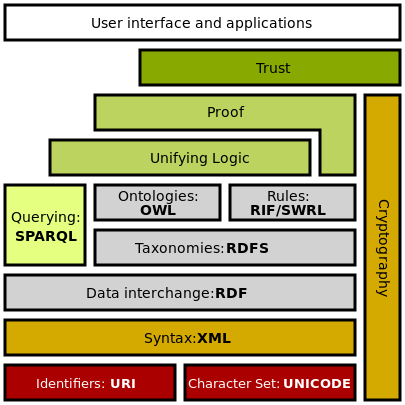
\includegraphics[width=0.75\linewidth]{img/Semantic_web_stack.png}
    \caption{Semantic Web Stack}
    \label{fig:bg:semantic-web-stack}
\end{figure}

\subsection{RDF, RDFS, and OWL}

\subsubsection{Resource Description Framework (RDF)}
The representation of semantics starts with specification of facts or `knowledge' using RDF\footnote{\url{https://www.w3.org/TR/rdf11-concepts/}}, which provides representation of information as `triples' whose collective expression can be visualised as a graph.
RDF triples are serialised using syntax languages such as XML\footnote{\url{https://www.w3.org/TR/rdf-syntax-grammar/}}, or the more human-readable Turtle\footnote{\url{https://www.w3.org/TR/turtle/}}, or the web friendly JSON-LD\footnote{\url{https://www.w3.org/TR/json-ld/}}.
RDF triples utilise the same identifier system as world wide web and are specified using IRIs\footnote{\url{https://tools.ietf.org/html/rfc3987}} - a generalised form of URIs which itself are a generalised form of URLs\footnote{\url{https://www.w3.org/TR/uri-clarification/}}.
A database storing RDF is called a triple-store and enables creation of graphs of RDF data and provides an interface for querying it.

A RDF triple consists of a subject, an object, and a predicate - where predicate describes the relationship from subject to object. An example of RDF triple specified using Turtle language to indicate chapter number of an entity is expressed as -\\ \-\hspace{5mm}\mintinline{turtle}{<http://example.com/ch2> foaf:name "Background"@en .}\\
The subject in this triple is the IRI \mintinline{turtle}{<http://example.com/ch2>} representing a resource, with the predicate \mintinline{turtle}{foaf:name} representing relationship of associating a name as indicated by the string in object field \mintinline{turtle}{"Background"@en} with \texttt{@en} specifying use of English language. 

The subject is written in shorthand notation indicating it starts with the same IRI as the data file it is described in. A complete IRI is often too long to write and is usually written using shorthand prefixes intended for human-readability.
The predicate is a \textit{property} provided by an external ontology called `Friend of a Friend' (FOAF\footnote{\url{http://xmlns.com/foaf/spec/}}), which is referenced by its prefix \texttt{foaf} as shorthand for its entire IRI.
The object is a string in this case, but could itself be another RDF triple or resource - in which case it would be specified as an IRI.

\subsubsection{RDF Schema (RDFS)}
RDFS provides concepts for expressing classes, properties, and data types in order to represent schemas using RDF. It also provides commonly required relationships such as specifying labels of resource, indicating related resource, or specifying domain and range of properties. The example in code below expands upon the triple described in RDF to express chapter as a class with its number as a property, and specifies human-readable labels for each resource.
\begin{minted}{turtle}
@prefix foaf: <http://xmlns.com/foaf/0.1/> .
@prefix : <http://example.com/> .
:Ch2 rdf:type :Chapter ; foaf:name "Background"@en ; :chnum 2^^xsd:integer .
:Chapter rdf:type rdfs:Class ; rdfs:label "Chapter"@en .
:chnum a rdfs:Property ; rdfs:label "number"@en ; rdfs:range xsd:integer .
\end{minted}

\subsubsection{Web Ontology Language (OWL)}
While RDFS enables expression of hierarchies, more formal representations of knowledge modelling and logic require additional constructs. These are represented using OWL\footnote{\url{https://www.w3.org/TR/owl2-overview/}} as an ontology consisting of set of `individuals' (also called classes) and a set of `property assertions' which relate individuals to each other.
An ontology may also consist of set of axioms which place constraints on sets of individuals and types of relationships permitted between them. These axioms provide semantics which can be used to infer additional information using semantic reasoners based on information explicitly provided.
Knowledge expressed using OWL can be (and generally is) expressed using RDF, which makes it possible to encode and store ontologies in as RDF data.

\subsection{SPARQL Protocol and RDF Query Language (SPARQL)}
SPARQL\footnote{\url{https://www.w3.org/TR/sparql11-query/}} is a query language for retrieving data expressed using semantics provided by RDF.
SPARQL queries information following the RDF specification, and thus specifies queries to act on data expressed as `subject-predicate-object' triples.
SPARQL queries can also retrieve information from traditional (SQL) databases which store data in non-RDF form through mapping\footnote{\url{https://www.w3.org/2008/07/MappingRules/StemMapping}} which permits its semantics to be applied across a large variety of existing data stores.

A SPARQL endpoint is an interface provided by a triple-store for access and querying over stored data. Such endpoints can be exposed over the web to provide querying capabilities through the internet, with DBPedia\footnote{\url{http://dbpedia.org/sparql}} - a semantic web representation of Wikipedia - providing a well-known example.

\subsection{Shapes Constraint Language (SHACL)}
SHACL\footnote{\url{http://dbpedia.org/sparql}} is a specification language for expressing constraints that validate RDF data. The input over which SHACL constraints are validated is called the \textit{data graph}.
Constraints in SHACL are called `shapes' based on the notion of checking if data \textit{fits a shape}, with the set of constraints being validated called as \textit{shapes graph}.
SHACL constraints are themselves also expressed in RDF which makes it possible to serialise them as a data graph and perform querying over it.

The output of validation process is a conformance report which uses a validation report vocabulary provided by SHACL and indicates \textit{failing validations} and status of validation of a whole. A \textit{conformance report} provides boolean indication of whether the any of given set of validations have failed or conversely whether all validations have passed.

\textit{SHACL-core} refers to features defined within SHACL standard specification. Extensions have been developed which provide additional features for expression and validation of constraints. Amongst these, \textit{SHACL-SPARQL} provides use of SPARQL queries to retrieve data failing a given constraint, and is mentioned within SHACL specification.
SHACL validations are performed using a `validator' - an implementation and interpretation of SHACL standard that provides at least the validation features described in SHACL-core.

\subsection{Standardised Ontologies}
\subsubsection{Provenance Ontology (PROV-O)}
PROV-O\footnote{\url{https://www.w3.org/TR/prov-o/}} is a standardised ontological representation of the PROV Data Model\footnote{\url{https://www.w3.org/TR/prov-dm/}} (PROV-DM) which is the W3C standard for representing provenance information using semantics provided by RDF and OWL.
PROV-O provides classes, properties, and restrictions to represent and interchange provenance information within different contexts.
It can be specialised to create new classes and properties to model provenance information for different applications and domains.

\subsubsection{Open Digital Rights Language (ODRL)}
ODRL\footnote{\url{https://www.w3.org/TR/odrl-model/}} is a policy expression language that provides an information model, vocabulary, and encoding mechanisms for representing statements about usage of content and services as policies. The ODRL Information Model describes underlying concepts, entities, and relationships that form the foundational basis for semantics of ODRL policies.
Policies are used to represent permitted and prohibited actions over one or more assets and can also contain obligations required to be met by stakeholders.
Policies can also specify constraints - such as temporal or spatial - and duties which are required to be carried out.
ODRL conformances is based on evaluating whether a given information representing an use-case or context satisfies all the expressions described in a given policy.
% \chapter{State of the Art}\label{chapter:sota}
% \chapter{Analysing GDPR Compliance Requirements}
\label{chapter:information}

The analysis of state of the art in \autoref{chapter:sota} provided identification of opportunities for addressing the gaps within it.
These opportunities relate to research objective $RO3$ regarding construction of ontologies, $RO4$ for querying, and $RO5$ for information validation.
In order to achieve these, it is imperative to have an understanding of GDPR and its compliance requirements as required by research objective $RO1$.
The requirement gathering process is shaped by the scope of research question - which for this thesis is representation of activities associated with processing of personal data and consent.
The identified requirements then need to be expressed in a form which will facilitate representation of information as ontologies, its querying, and validation in compliance process. This is required to fulfil research objective $RO2$.

The approaches presented in SotA in \autoref{chapter:sota} directly delve into obligations and requirements of data controllers to demonstrate compliance or towards data subject's consent and rights.
Since requirements of GDPR compliance are also influenced by other stakeholders such as processors and authorities which play an unspecified role in the context of information associated with compliance, such roles consist of interactions between stakeholders and involve communication of information such as instructions provided by a data controller to a processor.
Therefore, along with requirements of compliance, it is also important to understand interactions between stakeholders, information involved in such interactions, and requirements of information in terms of its interoperability between them.

As an example, consider a data controller that can have any number of internal representations of information necessary to demonstrate compliance, but an investigation by a supervisory body requires such information to be provided as per their stated requirements in an mutually understandable form. Furthermore, a processor contracted by a controller may also be required to present information relevant in investigation of compliance - which would also need to be mutually understandable by the processor, controller, and investigating authority.
When utilising technological solutions for management of compliance information, analysis of information interoperability requirements enable identifying applications of such solutions within a larger context comprised of multiple stakeholders involved in the compliance process.

This chapter therefore first presents an analysis of GDPR in terms of stakeholders and interoperability of information between them to construct a model of information interoperability in \autoref{sec:info:model}.
The model provides an analysis of requirements in terms of information and interoperability from the perspective of interactions between entities.
This provides an overview of information requirements which is used to find additional applications for existing information representation approaches and to identify gaps which can be addressed through future opportunities.
Such analyses and requirements gathering related to GDPR also benefit the larger community and domain by providing information for standardisation activities in understanding role of information and its interoperability between stakeholders, such as those for DPVCG (see \autoref{sec:intro:dpvcg}).

Following the above, \autoref{sec:info:compliance-questions} frames `compliance questions' that provide information requirements necessary to evaluate compliance, with its methodology presented in \autoref{sec:info:compliance-questions-methodology}, and \autoref{sec:info:constraints} presenting assumptions and constraints that can be used to validate information for correctness and completeness.
The use of compliance questions as competency questions in development and evaluation of ontologies is presented in \autoref{chapter:vocabularies}, and  use of constraints for validations is presented in \autoref{chapter:testing}.

\section{Interoperability Model of Information based on GDPR}\label{sec:info:model}
This section presents an analyses of GDPR in terms of interactions between stakeholders and information involved in such interactions. It then presents a model of interoperability for information associated with stakeholders. The model enables understanding role of stakeholders in compliance process in terms of information requirements and provides a framework to establish relationship between interactions and information required for compliance. 
The model also provides motivation to incorporate interoperability as a core requirement within representations of information towards GDPR compliance.
This provides context for development of ontologies presented in this thesis in terms of their intended application and usefulness to stakeholders associated with GDPR compliance.

The model serves to place contributions presented in this thesis within the larger context of stakeholders involved in GDPR compliance process. It does not have a direct impact on design of ontologies presented in \autoref{chapter:vocabularies}, but instead enables exploration of research question guiding this thesis regarding application of semantic web technologies for GDPR compliance.
In essence, it enables answering the question - ``Where can the contributions of this thesis prove useful in context of GDPR compliance?''.

The work described in this section was published within the interoperability and standardisation community as a conference paper
\cite{pandit_gdpr_2018} which was later expanded upon in a journal article \cite{pandit_exploration_2018} and a book chapter \cite{pandit_standardisation_2020}.

\subsection*{Interoperability Model}
The creation of model is based on identifying categories of entities as defined within GDPR and identifying interactions between them.
\autoref{fig:info:interoperability-model} visualises interactions between entities, and consists of Data Subject (DS), Data Controller (DC), Data Processor (DP) and Supervisory Authority\footnote{Supervisory Authority are also referred to as Data Protection Commission or Regulatory Body} (SA) as entities defined within GDPR.
The points of interactions consist of potential information exchange between entities and are guided by requirements of compliance. For example, interaction between data subject and data controller consists of data subject providing personal data to controller, while the controller is required to provide a copy of provided personal data for fulfilment of rights granted by GDPR.
\begin{figure}[htbp]
    \centering
    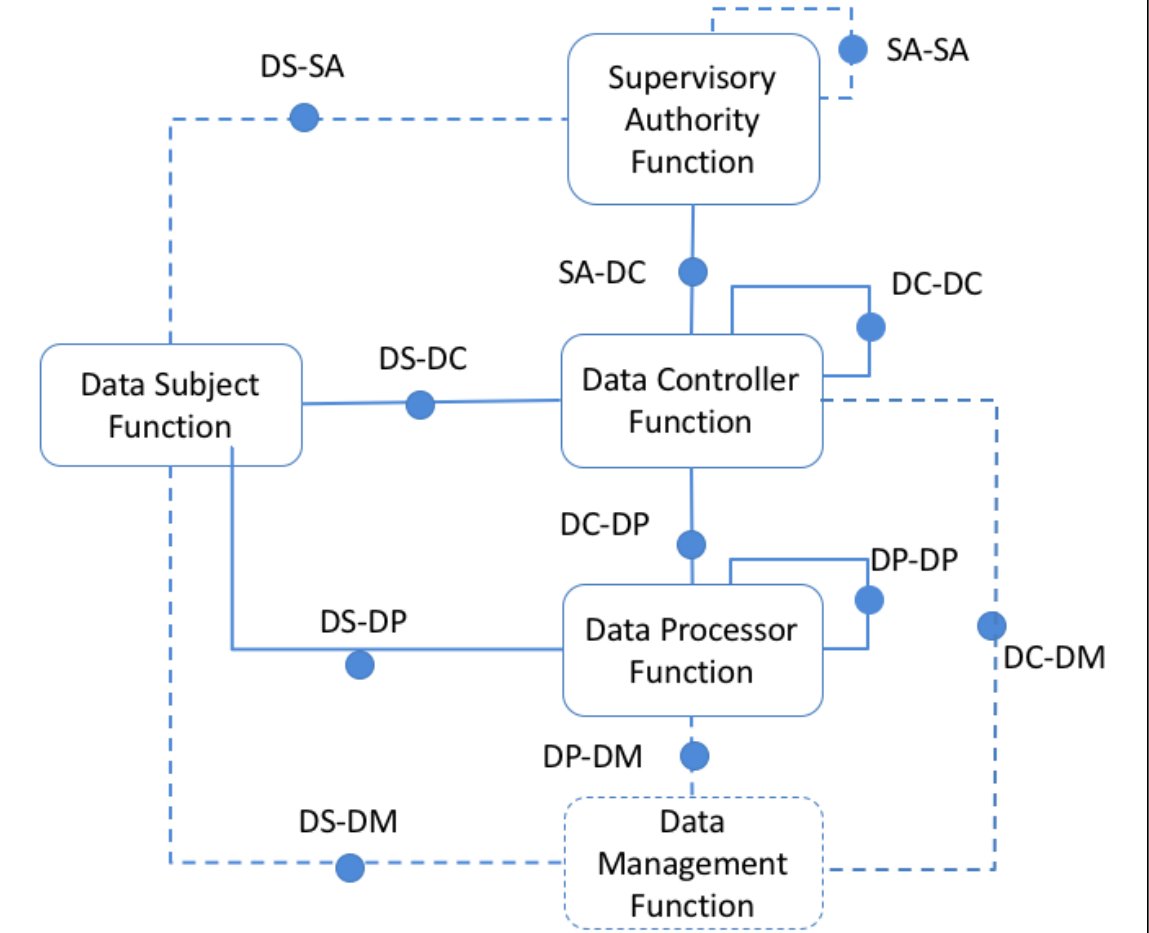
\includegraphics[width=0.75\linewidth]{img/interoperability-model.png}
    \caption{Interactions between entities based on requirements of GDPR \cite{pandit_exploration_2018}}
    \label{fig:info:interoperability-model}
\end{figure}

The model and information categories serve to provide a larger context of information requirements of GDPR and demonstrate areas for application of contributions presented in this thesis. They also provide future development and application of presented work to other areas of GDPR compliance. More specifically, they provide opportunities where developed work can be extended or re-applied to represent additional information regarding activities associated with GDPR compliance - such as for data breach records, carrying out rights, recording compliance procedures, or data processing agreements.

\subsection*{Information Categories}
The analyses of information flows between entities (additional description presented in publications \cite{pandit_exploration_2018,pandit_gdpr_2018}) provides categorises of information requirements as: provenance records, consent information, data processing agreements, compliance information, and seals/certifications - of which provenance records and consent have a direct bearing on the stated research objectives.
Carrying out further investigation and analyses of interactions and information involved is out of scope for research presented in this thesis given the focus of research question on information about activities associated with processing of personal data and consent.
To this end, analyses of information categories presented below concerns only categories of provenance and consent, and provides requirements for design of ontologies required by research objective $RO3$.

\subsubsection*{Provenance records}
Provenance in this case refers to information about entities and activities involved in the compliance process where a record is required to be kept and exchanged for compliance purposes. For example, GDPR requires controllers and processors to maintain provenance records of processing activities carried out under their responsibility in order to maintain and demonstrate compliance to supervisory authorities. Provenance records are also required to be maintained to enable provision of rights to data subjects, and for information sharing between controllers and third parties.

The information stored within provenance records is related to demonstrating compliant processing of personal data and fulfilment of obligations towards demonstration of compliance. They are modelled within state of the art (see \autoref{chapter:sota}) variously as logs, life-cycles, workflows, activities, and process flows. The term provenance in this case refers to both ex-ante and ex-post phases and is indicative of provenance of information to specify its existence. Therefore provenance in ex-ante phase means record of a model or plan used to indicate future processing of personal data, while that in ex-post phase refers to record or log of processing.

Since provenance information as described above encompasses information about artefacts and processes related to compliance, sharing this information in an interoperable format with other entities benefits both in their obligations regarding compliance. For example, controllers and supervisory authorities sharing interoperable compliance documentation can use the same set of tools and approaches for interacting with information. Also, by recording processes associated with compliance as provenance records, the same interoperable methods can be used to maintain, document, and demonstrate compliance. This is especially useful where information is to be shared between joint controllers and processors that need to exchange plans of processing for agreement as well as logs for successful implementations.

Since a data controller is required to ensure their intended activities are compliant as well as maintain records of processing activities regarding use of personal data, provenance records to be documented consist of intended plan of processing activities and their execution. Similarly, provenance records of consent requests and provision also need to be maintained to demonstrate compliance. Given the similarity in requirements for maintaining provenance records for different reasons, it is beneficial to provide a singular interoperable representation of provenance activities in a form that can capture and represent all aspects of provenance records required for compliance.

\subsubsection*{Consent information}
As per GDPR, consent is an assent or agreement by a data subject regarding processing of their personal data for specified purposes by one or more entities. 
For compliance, a controller must record information regarding how consent was requested and choices provided by a data subject as given consent.
GDPR has several obligations and requirements when it comes to valid consent, with additional requirements depending on sensitivity of personal data and processing. 
Artefacts associated with choices offered for consent therefore need to be preserved to demonstrate the validity of consent obtained using those choices.
Similarly, consent revocation or revisions also need to be recorded and linked to earlier instances of consent to demonstrate a change was valid as per requirements of GDPR.

The processes associated with offering consent choices, retrieving and recording given consent, enabling withdrawal of consent, and executing revocation in internal processes need to be documented for compliance by relevant controller(s).
These are associated across both ex-ante and ex-post phases where consent choices, provision of right to withdrawal, and demonstrating utilisation of consent in processing are demonstrated as ex-ante measures while given consent and revoked consent are ex-post artefacts. 

If consent is considered as an instance of personal data, the same information model used to document processing of personal data can be re-purposed or reused to represent activities associated with consent. In addition to this, activities need to capture different stages of consent and personal data by representing their life-cycles which involve processes and artefacts which use them or are dependant on them to indicate their evolution and use over time. 

\subsubsection*{Stating interoperability as a requirement}
The model and analyses of information flows between entities provides motivation for establishing interoperability in representation of information to be exchanged.
As the scope of thesis focuses on representation of activities associated with processing of personal data and consent, requirements gathered from this analysis relate primarily to information associated with provenance of activities and information about consent.
Within this scope, ensuring potential reuse towards other categories through future extensions is provided by developing an interoperable ontology by using standards that can be utilised to also represent data processing agreements and compliance agreements in the future.
This involves using standards of RDF and OWL2 to represent ontologies along with reuse of existing standardised vocabularies such as PROV-O and ELI.
In addition, the research also provides transparency by using terminology of GDPR in developed ontologies, indicating requirements used to shape design of ontology and indicating source of concepts within GDPR.

Representing provenance is not limited to representation of processing of personal data, but is also applicable to information about other categories - consent, data processing agreements, compliance, and certifications. Therefore, utilising the same or compatible representation in representing provenance across all use-cases has advantage towards cohesive management of all associated information for compliance - and provides an objective for future work in expanding contributions presented in this thesis.

With this motivation, the next parts of this chapter provide requirements gathered for representing information regarding processing of personal data and consent while also including other relevant information such as data breaches and provision of rights to indicate potential applicability and reuse of developed ontologies in representing information through provenance records for GDPR compliance.

\section{Compliance Questions}\label{sec:info:compliance-questions}
This section presents `compliance questions' whose answers provide information necessary for evaluating GDPR compliance. The questions are essential to development of information representations within compliance management systems by providing requirements for structuring of information and its validation. Within this thesis, they are used to guide development of ontologies as competency questions (see \autoref{chapter:vocabularies}) and validation of information (see \autoref{chapter:testing}). \textbf{The questions presented here are by no means exhaustive but represent gathered requirements from authoritative sources.} As supervisory authorities and courts continue to clarify and interpret compliance requirements of GDPR, these questions are expected to change and expand in future.

\subsection{Methodology}\label{sec:info:compliance-questions-methodology}
The questions were created by studying authoritative sources regarding GDPR compliance consisting of data protection commissions, legal experts and agencies - that have published guidelines and resources to assist organisations with the process of establishing and maintaining GDPR compliance.
In this process, each identified clause or article of GDPR pertaining to the research question was formulated as a question, with the above mentioned sources providing indication on how the question should be interpreted and  requirements for its compliance.
The questions were derived from reading and understanding of compliance requirements and are intentionally expressed as a `simple question' whose answering requires minimal information in order to determine requirements of such information towards constructing an ontological representation of it.
% As questions were formulated from an understanding of GDPR, they are associated with specific clauses where a question was derived explicitly from particular clauses.

For questions presented in this thesis, following sources were used or referenced in addition to text of GDPR:
\begin{itemize}
    \item Guidelines, clarifications, and discussions on interpretation of GDPR published by European Data Protection Board\footnote{\url{https://edpb.europa.eu/}} (EDPB)
    \item Guidelines, clarifications, and discussions on interpretation of GDPR published by Article 29 Working Party\footnote{\url{https://ec.europa.eu/newsroom/article29/news.cfm?item_type=1360}} and endorsed by EDPB
    \item Resources published Data Protection Commission\footnote{\url{https://dataprotection.ie/}} (Ireland) - with particular focus on document `GDPR guidance for SMEs'\footnote{\url{https://dataprotection.ie/en/guidance-landing/guidance-smes}}
    \item Resources published by Information Commissioners Office\footnote{\url{https://dataprotection.ie/}} (United Kingdom), with particular use of `Data protection self assessment for organisations'\footnote{\url{https://ico.org.uk/for-organisations/data-protection-self-assessment/}}
    \item Resources published by federated data protection offices in Germany, in particular the audit checklist published by Lower Saxony Data Protection Authority\footnote{\url{https://lfd.niedersachsen.de/download/146715/}} self-translated from German to English\footnote{\url{https://doi.org/10.5281/zenodo.3380469}}
    \item Resources regarding GDPR compliance published by professional institutions within legal compliance domain, specifically - Nymity\footnote{\url{https://info.nymity.com/gdpr-compliance-toolkit}} and IAPP\footnote{\url{https://iapp.org/resources/article/gdpr-genius/}}
    \item Executive and Court decisions regarding GDPR compliance, tracked through an online community service \url{https://www.enforcementtracker.com/} which also denotes relevant articles of GDPR
\end{itemize}

The questions pertaining to consent and its associated processing activities were validated through consultation with a law professor at Trinity College Dublin who served as a legal domain expert and validated the questions and information required to answer them. This consisted of providing a spreadsheet containing categories of questions along with their assumptions and constraints as information requirements, with the feedback consisting of whether stated information was correct, utilised correct terminology, and changes in statements to suit legal interpretations.
Other questions pertaining to processor obligations, data breach requirements, and rights were not validated through this process due to unavailability of expert and their lower priority in relevance to the research question.

The author of this thesis was part of an informal consultation on a real-world (details confidential) research project at MasterCard regarding creation of a semantic web ontology for expressing consent information based on requirements of the GDPR.
The consultation consisted of identifying information for representing consent based on requirements of GDPR and designing an ontology to represent it. 
This process provided real-world requirements about management of consent information which had an influence on compliance questions associated with consent and design of GConsent ontology presented in \autoref{sec:voc:GConsent}.

The collected questions were rephrased and divided into smaller more granular questions towards establishment of information requirements and constraints. 
Each question was assigned an ID to enable tracking its use.
Where possible, each question was associated with specific clauses of GDPR by denoting an article or recital relevant to it. Each question was analysed in terms of information requirements to identify assumptions that clarify interpretation of the question, and constraints that express a condition that can be tested and used to validate information. For each identified constraint, a failing test case was identified that did not satisfy the condition and could be used to test its validation.
% \todo{upload all documents to Zenodo and put link here}
% A spreadsheet was used to collect and organise the questions, assumptions, and constraints - and is available as an open resource\footnote{\url{TODO: upload spreadsheet to Zenodo and post link here}}.

The list of questions is presented in \autoref{sec:info:compliance-questions-list} with assumptions and constraints presented in \autoref{sec:info:constraints}. Along with compliance questions regarding activities associated with processing of personal data and consent, the list also contains questions about additional activities associated with right to be informed and reporting of data breach by controllers. These questions are used in development of ontologies that demonstrate application of a common approach to represent activities related to processing of personal data, consent, data breach, and provision of rights for GDPR compliance. 

\subsection{List of Questions}\label{sec:info:compliance-questions-list}
The questions are categorised based on the topic they focus on within the context of compliance. Where a question was directly derived from specific clause(s) a reference to the clause(s) is provided at end of sentence\footnote{Shortened references are used to indicate the clause of GDPR. For example: R32 indicates Recital 32, A7-2 indicates Article 7 Para 2, and A9-2c indicates Article 9 Para 2 Sub-Para c.}.
In order to provide a context for application of questions within real world, a group of use-cases are provided in \autoref{sec:info:use-cases}.
An overview of compliance questions and their categorisation as follows:
\begin{itemize}
	\item \autoref{sec:info:CQ:1} Compliance questions pertaining to records of processing activities to be kept by controllers: \texttt{CMQ.1 - CMQ.15}.
	\item \autoref{sec:info:CQ:2} Compliance questions pertaining to records of processing activities to be kept by processors: \texttt{CMQ.16 - CMQ.25}.
	\item \autoref{sec:info:CQ:3} Compliance questions pertaining to legal basis of processing activities: \texttt{CMQ.26 - CMQ.27}.
	\item \autoref{sec:info:CQ:4} Compliance questions pertaining to personal data: \texttt{CMQ.28 - CMQ.34}.
	\item \autoref{sec:info:CQ:5} Compliance questions pertaining to given consent: \texttt{CMQ.35 - CMQ.69}.
	\item \autoref{sec:info:CQ:6} Compliance questions pertaining to change in consent state: \texttt{CMQ.70 - CMQ.87}.
	\item \autoref{sec:info:CQ:7} Compliance questions pertaining to provision of right to be informed: \texttt{CMQ.88 - CMQ.105}.
	\item \autoref{sec:info:CQ:8} Compliance questions pertaining to reporting of data breach by controllers: \texttt{CMQ.106 - CMQ.120}.
\end{itemize} 

\subsubsection{Use-cases}\label{sec:info:use-cases}
To identify application of compliance questions in various scenarios within real world, 15 categories of use-cases were identified to determine necessary information required to identify their ontological representations.
The use-cases are based on identifying information affecting compliance requirements and identifying variances which affect representations of that information.
These were useful to guide development of ontologies by serving as test scenarios where an ontology could be applied and evaluated for representing information.
These use-cases are not intended to be comprehensive or normative from a legal compliance point of view, but are helpful in understanding presented work by providing a context for their application.

A summary of these use-cases is as follow:
\begin{enumerate}
% \tightlist
\item
  Obtaining / Declaring Consent (its state)

  \begin{enumerate}
%   \tightlist
  \item
    The consent is given
  \item
    Consent was given, but is now invalidated (by the controller)
  \item
    Consent was given, but was withdrawn (by the Data Subject)
  \item
    Consent was requested (by the controller)
  \item
    Consent was requested, but was refused (by the Data Subject)
  \item
    Consent state is unknown (e.g. when importing data about consent)
  \end{enumerate}
\item
  Entity the consent is about

  \begin{enumerate}
%   \tightlist
  \item
    The consent is about a Data Subject who is not a minor
  \item
    The consent is about a Data Subject who is a minor
  \end{enumerate}
\item
  Activity for Data Subject

  \begin{enumerate}
%   \tightlist
  \item
    There was an age verification process associated with the consent
    (such as for minors)
  \item
    There was an identity verification process associated with the
    consent
  \end{enumerate}
\item
  Entity that provided consent

  \begin{enumerate}
%   \tightlist
  \item
    Consent was provided by the Data Subject it is about
  \item
    Consent was not provided by the Data Subject it is about, but was
    provided by a Delegation

    \begin{enumerate}
    % \tightlist
    \item
      Consent in the Delegation was provided by another Data Subject
    \item
      Consent in the Delegation was provided by a Person
    \item
      Consent in the Delegation was provided by another Delegation
    \end{enumerate}
  \end{enumerate}
\item
  Role within Delegation

  \begin{enumerate}
%   \tightlist
  \item
    Entity is the Parent/Guardian of the Data Subject
  \item
    Entity is a third-party to the Data Subject
  \end{enumerate}
\item
  Activity of Delegation

  \begin{enumerate}
%   \tightlist
  \item There was some verification process to assert the authentication of
    the delegation
  \end{enumerate}
\item
  Personal Data associated with consent

  \begin{enumerate}
%   \tightlist
  \item
    Consent was given for specific instances of personal data e.g. John/Jane Doe
  \item
    Consent was given for categories of personal data e.g. Name
  \end{enumerate}
\item
  Medium of Consent

  \begin{enumerate}
%   \tightlist
  \item
    consent is given via a web-form
  \item
    consent is given as a signed paper document
  \item
    consent is given as a verbal confirmation
  \item
    consent is given implicitly in some form (medium)
  \item
    consent is given via delegation in some form (medium)
  \end{enumerate}
\item
  Activity responsible for consent

  \begin{enumerate}
%   \tightlist
  \item
    Activity created consent as a new entity
  \item
    Activity modified existing consent
  \end{enumerate}
\item
  Previous consent and relationship

  \begin{enumerate}
%   \tightlist
  \item
    Consent has no previous instance
  \item
    Consent has a previous instance and replaces it
  \end{enumerate}
\item
  Differences between consent instances

  \begin{enumerate}
%   \tightlist
  \item
    Something changes between two consent instances (e.g. personal data
    category is added)
  \end{enumerate}
\item
  Time constraints

  \begin{enumerate}
%   \tightlist
  \item
    consent expires (has a tangible expiry such as a specific date or
    duration)
  \item
    consent does not expire (is valid for ``as long as required'')
  \end{enumerate}
\item
  Third party Association

  \begin{enumerate}
%   \tightlist
  \item
    Personal Data is collected from a third party
  \item
    Personal Data is stored with a third party (processor)
  \item
    Personal Data is shared with a third party
  \item
    Processing involves third party
  \item
    Purpose involves third party
  \end{enumerate}
\item
  Role of Third Party

  \begin{enumerate}
%   \tightlist
  \item
    Third Party is a Processor contracted by the Controller
  \item
    Third Party is another Controller
  \item
    Third Party is another entity (regulatory/supervisory/governmental)
  \end{enumerate}
\item
  Storage Duration and Locations for Personal Data

  \begin{enumerate}
%   \tightlist
  \item
    Data is stored for a fixed time (specific instance or duration)
  \item
    Data is stored for an indefinite duration (``for as long as
    required'')
  \end{enumerate}
\end{enumerate}

% COMPLIANCCE QUESTIONS - CONTROLLERS
\subsubsection{Compliance questions pertaining to records of processing activities to be kept by controllers}\label{sec:info:CQ:1}
\begin{enumerate}[label={\textit{CMQ.\theenumi}}]
    \item How are the records of processing activities maintained? (R82,A30,A30-3)
    \item What is the name and identity of the controller(s) and their representatives/DPOs? (A30-1a)
    \item What are the the purposes of processing? (A30-1b)
    \item What are the categories of data subjects? (A30-1c)
    \item What are the categories of personal data? (A30-1c)
    \item Is data shared?
    \item If data is shared, what are the categories of recipients to whom the personal data is or will be disclosed? (A30-1d)
    \item If data is shared, what are the identities of the recipients to whom the data is or will be disclosed? (A30-1d,A30-1e)
    \item If data is shared, are the recipients to whom the data is or will be disclosed based in a Third Country or International Organisation? (A30-1e)
    \item If data is shared, and the recipients are in a Third Country or International Organisation, what are the safeguards associated with data transfer? (A30-1e)
    \item Is data stored?
    \item Where data is stored, its erasure is based on what criteria: time limit or condition or event?
    \item Where data is stored, what are the time limits or conditions or events for erasure for different categories of data? (A30-1f)
    \item What are the technical and organisational security measures w.r.t to the processing of personal data? (A30-1g)
    \item Where data is shared, what are the purposes for sharing of personal data with the recipients?
\end{enumerate}

% COMPLIANCE QUESTIONS - PROCESSORS
\subsubsection{Compliance questions pertaining to records of processing activities to be kept by processors}\label{sec:info:CQ:2}
\begin{enumerate}[label={\textit{CMQ.\theenumi}},resume]
    \item How are the records of processing activities maintained? (R82,A30,A30-3)
    \item What is the name and identity of the processor(s) and their representatives/DPOs? (A30-1a)
    \item What is the name and identity of the controller(s) the processor is acting on behalf of? (A30-2a)
    \item What are the the categories of processing carried out on behalf of the controller? (A30-2b)
    \item If data is shared, what are the categories of recipients to whom the personal data is or will be disclosed? (A30-1d)
    \item If data is shared, what are the identities of the recipients to whom the data is or will be disclosed? (A30-1d,A30-1e)
    \item If data is shared, are the recipients to whom the data is or will be disclosed based in a Third Country or International Organisation? (A30-1e)
    \item If data is shared, and the recipients are in a Third Country or International Organisation, what are the safeguards associated with data transfer? (A30-1e)
    \item What are the technical and organisational security measures w.r.t to the processing of personal data? (A30-1g)
    \item Where data is shared, what are the purposes for sharing of personal data with the recipients?
\end{enumerate}
% COMPLIANCE QUESTIONS - LEGAL BASIS
\subsubsection{Compliance questions pertaining to legal basis of processing activities}\label{sec:info:CQ:3}
\begin{enumerate}[label={\textit{CMQ.\theenumi}},resume]
    \item What is the legal basis for processing of data?
    \item What is the legal basis for the purpose for processing of data?
\end{enumerate}

% COMPLIANCE QUESTIONS - PERSONAL DATA
\subsubsection{Compliance questions pertaining to personal data}\label{sec:info:CQ:4}
\begin{enumerate}[label={\textit{CMQ.\theenumi}},resume]
    \item What are the sources of personal data?
    \item What personal data are collected from the data subject?
    \item Where personal data are not collected from the data subject, what are their sources?
    \item Where data has been anonymised, what techniques were used for anonymisation?
    \item Can pseudo-anonymised data be de-anonymised by the organisation using information it already possesses or is available to it?
    \item Where personal data is collected, is it pseudo-anonymous?
    \item What are the special categories of personal data being processed?
\end{enumerate}

% COMPLIANCE QUESTIONS - GIVEN CONSENT
\subsubsection{Compliance questions pertaining to given consent}\label{sec:info:CQ:5}
\begin{enumerate}[label={\textit{CMQ.\theenumi}},resume]
    \item Who is the Data Subject associated with consent? (A4-11)
    \item What are the Personal Data associated with consent? (R32,A4-11)
    \item What are the Purposes associated with consent? (R32,R42)
    \item What are the Data Processing associated with consent? (R32,A4-11)
    \item What is the current Status of consent? (A7-3)
    \item Who are the Data Controllers associated with consent?
    \item Who provided consent? (A7-2)
    \item Was consent provided by Delegation? (A8-c)
    \item If consent was provided by Delegation, what was the role played by Delegate with respect to the Data Subject?
    \item If consent was provided by Delegation, how was the delegation executed?
    \item If consent was provided by Delegation, how was the delegate authenticated? (A8-2)
    \item Who was the consent given to?
    \item If consent was not given to the Data Controller, what is the relationship between the entity it was provided to and the Data Controller?
    \item How was the consent given/obtained?
    \item What artefacts were involved in the giving/obtaining of consent?
    \item What were the choices provided for consent?
    \item What was the statement or affirmative action indicating given consent?
    \item How was the right to withdraw consent communicated to the data subject?
    \item At what location was the consent given?
    \item What is the medium associated with consent? (R32,A7-2)
    \item What is the timestamp associated with the consent?
    \item What is the expiry of the consent?
    \item Is the purpose or processing associated with a third party?
    \item What is the role played by the third party in the purpose or processing?
    \item Does the processing of data involve storage of data?
    \item If personal data is being stored, what is the duration of storage for Personal Data?
    \item If personal data is being stored, what is the location of storage?
    \item Are processing associated with consent of automated nature? (R71,A9-2c,A22-2c)
    \item Does the processing of data involve transfer to a Third Country or International Organisation? (R111,A49-1a)
    \item If processing of data involves transfer to a Third Country or International Organisation, what is the identity of the Third Country or International Organisation?
    \item Do the personal data associated with consent belong to a special category? (R51,A8-2a)
    \item How is personal data associated or linked to the data subject?
    \item Is the Data Subject of legal age to provide their own consent? (A8)
    \item What are the specific laws that determine the legal age to provide consent? (A8-1)
    \item Does the Data Subject have a specific relationship with the Data Controller? (R43)
\end{enumerate}

% COMPLIANCE QUESTIONS - CHANGE IN CONSENT STATE
\subsubsection{Compliance questions pertaining to change in consent state}\label{sec:info:CQ:6}
In this, the definition of change in consent is where the state/status of consent is changed. Example: unknown to not asked or not given, from given to withdrawn, from given to invalidated. Changes where the result is given consent or obtained consent where none existed is considered as given consent with compliance questions listed in the previous section.
\begin{enumerate}[label={\textit{CMQ.\theenumi}},resume]
    \item Who is the Data Subject associated with consent? (A4-11)
    \item What are the Personal Data associated with consent? (R32,A4-11)
    \item What are the Purposes associated with consent? (R32,R42)
    \item What are the Data Processing associated with consent? (R32,A4-11)
    \item What is the current state/status of consent? (A7-3)
    \item Who are the Data Controllers associated with consent?
    \item Who changed the state/status of consent?
    \item Was consent changed by Delegation?
    \item If consent was changed by Delegation, what was the role played by Delegate with respect to the Data Subject?
    \item If consent was changed by Delegation, how was the delegation executed?
    \item If consent was changed by Delegation, how was the delegate authenticated? (A8-2)
    \item How was the consent state/status changed?
    \item What artefacts were involved in the change in state/status of consent?
    \item If change in consent was done by the Data Subject, what was the statement or affirmative action indicating change to their consent?
    \item At what location was the consent changed?
    \item What is the medium associated with change in consent? (R32,A7-2)
    \item What is the timestamp associated with the consent?
    \item If the current state/status of consent is valid for processing, what is the expiry of the consent?
\end{enumerate}

% COMPLIANCE QUESTIONS - RIGHT TO BE INFORMED
\subsubsection{Compliance questions pertaining to provision of right to be informed}\label{sec:info:CQ:7}
\begin{enumerate}[label={\textit{CMQ.\theenumi}},resume]
    \item How was information relevant for the right to be informed provided to the data subjects?
    \item When was the information relevant to right to be informed was provided to the data subject?
    \item Was the name and contact details of the controller’s representative provided to the data subject under the right to be informed?
    \item Was the name and contact details of the DPO provided to the data subject under the right to be informed?
    \item Was the purposes for processing provided to the data subject under the right to be informed?
    \item Was the legal basis for processing provided to the data subject under the right to be informed?
    \item Where the legal basis for processing was legitimate interest, was this communicated to the data subject under the right to be informed?
    \item If personal data is not obtained from the data subject, were the categories of personal data obtained communicated to the data subject under the right to be informed?
    \item If personal data is not obtained from the data subject, were the sources of data communicated to the data subject under the right to be informed?
    \item Where personal data is shared, were the recipients or categories of recipients communicated to the data subject under the right to be informed?
    \item If personal data is transferred to a third country or international organisation, were the identity of the third country or international organisation communicated to the data subject under the right to be informed?
    \item Where personal data is stored, were the retention period communicated to the data subject under the right to be informed?
    \item Were the rights available communicated to the data subject under the right to be informed?
    \item If the data subject provided consent, was the right to withdraw consent provided under the right to be informed?
    \item Was the right to lodge a complaint with a supervisory authority provided to the data subject under the right to be informed?
    \item Where personal data needs to be provided under statutory or contractual obligation, was this communicated to the data subject under the right to be informed?
    \item Where personal data needs to be provided under statutory or contractual obligation, and if this data needs to be obtained from the data subject, was this communicated to the data subject under the right to be informed?
    \item Where automated-decision making, including profiling is used, was this communicated to the data subject under the right to be informed?
\end{enumerate}

% COMPLIANCE QUESTIONS - DATA BREACH
\subsubsection{Compliance questions pertaining to reporting of data breach by controllers}\label{sec:info:CQ:8}
\begin{enumerate}[label={\textit{CMQ.\theenumi}},resume]
    \item When did the data breach occur?
    \item When did the controller become aware of the data breach? (R85,R33-1)
    \item Was the data breach notified to the supervisory authority?
    \item When was the notification of data breach provided to the supervisory authority? (R85)
    \item How was the notification of data breach provided to the supervisory authority? (R85,R33-1)
    \item Is the data breach likely to result in a high risk to the rights and freedoms of the natural person whose data is associated with it? (R86,A33-1,A34-1)
    \item Who are the data subjects whose personal data are associated with the data breach?
    \item Was the data breach notified to the data subjects?
    \item When was the notification of data breach provided to the data subjects?
    \item How was the notification of data breach provided to the data subjects? (R85,R33-1)
    \item How did the notification of data breach to the data subject provide information about the data breach? (R86,A34-2)
    \item How did the notification of data breach to the data subject provide information about mitigating potential effects? (R86,A34-2)
    \item What data was involved in the data breach?
    \item What technical measures were in place for the protection of data involved in the data breach? (R88)
    \item What steps were taken to prevent or mitigate the effects of the data breach?
\end{enumerate}

\subsection{Assumptions \& Constraints}\label{sec:info:constraints}
An assumption is defined as information or condition that always holds true and is useful in the interpretation of the compliance question. A constraint is defined as a condition that the information pertaining to compliance question must satisfy in order for it to be valid. The assumptions and constraints are listed with reference to the relevant compliance question at the end in brackets.
An overview of the assumptions and constraints based on the categories of compliance questions is as follows:
\begin{itemize}
	\item \autoref{sec:info:CQ:1} Compliance questions pertaining to records of processing activities to be kept by controllers: \texttt{CMQ.1 - CMQ.15}  has Assumptions \texttt{A.1 - A.5} and Constraints \texttt{C.1 - C.18}
	\item \autoref{sec:info:CQ:2} Compliance questions pertaining to records of processing activities to be kept by processors: \texttt{CMQ.16 - CMQ.25} has Constraints \texttt{C.16 - C.32}
	\item \autoref{sec:info:CQ:3} Compliance questions pertaining to legal basis of processing activities: \texttt{CMQ.26 - CMQ.27}  has Assumptions \texttt{A.6} and Constraints \texttt{C.33 - C.34}
	\item \autoref{sec:info:CQ:4} Compliance questions pertaining to personal data: \texttt{CMQ.28 - CMQ.34}  has Assumptions \texttt{A.7} and Constraints \texttt{C.35 - C.38}
	\item \autoref{sec:info:CQ:5} Compliance questions pertaining to given consent: \texttt{CMQ.35 - CMQ.69}  has Assumptions \texttt{A.8 - A.28} and Constraints \texttt{C.39 - C.69}
	\item \autoref{sec:info:CQ:6} Compliance questions pertaining to change in consent state: \texttt{CMQ.70 - CMQ.87}  has Assumptions \texttt{A.30 - A.39} and Constraints \texttt{C.70 - C.87}
	\item \autoref{sec:info:CQ:7} Compliance questions pertaining to provision of right to be informed: \texttt{CMQ.88 - CMQ.105} has Constraints \texttt{C.88 - C.113}
	\item \autoref{sec:info:CQ:8} Compliance questions pertaining to reporting of data breach by controllers: \texttt{CMQ.106 - CMQ.120} has Constraints \texttt{C.114 - C.130}
\end{itemize} 

\subsubsection{Assumptions}
\begin{enumerate}[label={\textit{A.\theenumi}}]
    \item Processing activities as a whole can involve multiple controllers - (CMQ2)
    \item Data recipient categories refer to a collection or abstraction of recipients based on some context such as purpose e.g. “our ad partners” or requirement e.g. “law agencies” - (CMQ8)
    \item Data recipients cannot be a collective or a group whose identity cannot be represented as a list of its members e.g. “our partners” vs “our partners – A, B, C” - (CMQ9)
    \item Identity of the recipients does not need to be associated with the processing record if category of recipients is already documented. However, the identity of recipients within the category at that point of time must be recorded (somewhere). - (CMQ10)
    \item Where data is stored, its erasure can depend on a condition or an event e.g. “XX days after your last sign-in”, or “as long as your account is active” - (CMQ12)
    \item Processing carried out for a specific purpose adopts the legal basis of the purpose - (CMQ26)
    \item Personal data may not have the source information associated with it directly. It must have some link (chain, path) to the information and its source from which it was obtained. - (CMQ28)
    \item If there are multiple categories of personal data, consent is granted for all (union) of them - (CMQ36)
    \item If a consent is given for multiple purposes, consent is considered given for all (union) of them - (CMQ37)
    \item If a consent is given for multiple processing, consent is considered given for all (union) of them - (CMQ38)
    \item Valid status of consent are when it is given (explicitly or implicitly) by the data subject, or by delegation - (CMQ39)
    \item Invalid status of consent are when it its status is unknown, refused, not offered, withdrawn, invalidated, terminated, or expired. - (CMQ39)
    \item The status of consent indicates whether it can be used as a legal basis for processing - (CMQ39)
    \item Consent provided by a Person that is not the Data Subject is consent by Delegation - (CMQ41)
    \item A delegation can involve another delegation for the provision of consent - (CMQ42)
    \item If consent is provided to an actor not the data controller associated with consent, the actor is considered as acting on behalf of the controller - (CMQ46)
    \item Specifying location for obtained consent is optional - (CMQ53)
    \item Specifying medium for obtained consent is optional - (CMQ54)
    \item Consent may not have a tangible expiry - (CMQ56)
    \item Consent may have multiple forms of expiry depending on conditions or events - (CMQ56)
    \item A purpose or processing may be associated with zero or more third parties - (CMQ57)
    \item Processing of data may involve storage of data - (CMQ59)
    \item Different personal data, processing, or purpose may have different storage of data - (CMQ60)
    \item Storage duration may not be a tangible instance in time, it can depend on conditions or event - (CMQ60)
    \item Processing may involve transfer of data to a third country or international organisation - (CMQ63)
    \item Personal data associated with consent may belong to a special category - (CMQ65)
    \item A data subject may be a minor or a child - (CMQ67)
    \item The data subject may have a relationship of relevance with the Data Controller - (CMQ69)
    \item If there are multiple categories of personal data, consent is granted for all (union) of them - (CMQ71)
    \item If a consent is given for multiple purposes, consent is considered given for all (union) of them - (CMQ72)
    \item If a consent is given for multiple processing, consent is considered given for all (union) of them - (CMQ73)
    \item Valid status of consent are when it is given (explicitly or implicitly) by the data subject, or by delegation - (CMQ74)
    \item Invalid status of consent are when it its status is unknown, refused, not offered, withdrawn, invalidated, terminated, or expired. - (CMQ74)
    \item The status of consent indicates whether it can be used as a legal basis for processing - (CMQ74)
    \item Consent state/status can be changed by Delegation - (CMQ76)
    \item A delegation can involve another delegation for the provision of consent - (CMQ77)
    \item Specifying location for changed consent is optional - (CMQ84)
    \item Specifying medium for changed consent is optional - (CMQ85)
    \item Consent may not have a tangible expiry - (CMQ87)
    \item Consent may have multiple forms of expiry depending on conditions or events - (CMQ87)
\end{enumerate}

\subsubsection{Constraints}
\begin{enumerate}[label={\textit{C.\theenumi}}]
    \item Processing carried out by a controller must have information on how its records are being maintained - (CMQ1)
    \item Records of processing activity under the responsibility of a controller must have the names/identity of all associated controllers - (CMQ2)
    \item Each controller associated record of processing activities under the responsibility of (this) controller must have one or more contact details - (CMQ3)
    \item Each controller associated with records of processing activities under the responsibility of (this) controller must have the identity and one or more contact details of the DPO - (CMQ4)
    \item Processing under the responsibility of a controller must have one or more purposes of processing associated with it - (CMQ3)
    \item Processing under the responsibility of a controller must have one or more categories of data subjects associated with it - (CMQ4)
    \item Processing under the responsibility of a controller must have one or more categories of personal data associated with it - (CMQ5)
    \item Processing under the responsibility of a controller must explicitly state when data is shared - (CMQ6)
    \item Processing under the responsibility of a controller where data is shared must have the category of recipients to whom the data is or will be disclosed - (CMQ7)
    \item Processing under the responsibility of a controller where data is shared must have the identities of recipients to whom the data is or will be disclosed - (CMQ8)
    \item Processing under the responsibility of a controller where the recipients to whom the data is or will be disclosed are based in a Third Country or International Organisation must explicitly specified it as such - (CMQ9)
    \item Processing under the responsibility of a controller must specify the identity of the Third Country or International Organisation to whom the data is or will be disclosed - (CMQ10)
    \item Processing under the responsibility of a controller where personal data is transferred to a third country or an international organisation must specify the safeguards present for the transfer - (CMQ10)
    \item Processing under the responsibility of a controller must explicitly state when data is stored - (CMQ11)
    \item Processing under the responsibility of a controller where data is stored must specify the criteria for its erasure - (CMQ12)
    \item Each category of data associated with a record of processing must have a time limit or a condition or an event specified for its erasure - (CMQ13)
    \item The record of processing must have technical and organisational security measures associated with it - (CMQ14)
    \item Every sharing of personal data must specify the purposes of sharing with the recipients - (CMQ15)
    \item Every processing must have information on how its records are being maintained - (CMQ16)
    \item Each record of processing activity under the responsibility of a processor must have the names/identity of all associated processors under its responsibility - (CMQ17)
    \item Each processor associated with a record of processing activity under the responsibility of a processor must have one or more contact details - (CMQ17)
    \item Each processor associated with a record of processing activity under the responsibility of a processor must have the identity and one or more contact details of the DPO - (CMQ17)
    \item Each record of processing activity under the responsibility of a processor must have the names/identity of the controller(s) it is acting on behalf of - (CMQ18)
    \item Each record of processing activity under the responsibility of a processor must have name and contact details of the controller's representative and DPO - (CMQ18)
    \item Each record of processing carried out by a processor on behalf of a controller must specify categories of processing associated with it - (CMQ19)
    \item Each record of processing under the responsibility of a processor where data is shared must have the identity of recipients to whom the data is or will be disclosed - (CMQ20)
    \item The identities of the recipients to whom data is or will be disclosed must be specified - (CMQ21)
    \item If the recipients to whom the data is or will be disclosed are based in a Third Country, or International Organisation, this must be specified as such - (CMQ22)
    \item The identity of the Third Country or International Organisation to whom the data is or will be disclosed must be specified - (CMQ22)
    \item The transfer of personal data to a third country or an international organisation must specify its safeguards - (CMQ23)
    \item The record of processing must have technical and organisational security measures associated with it - (CMQ24)
    \item Every sharing of personal data must specify the purposes of sharing with the recipients - (CMQ25)
    \item Each processing of data must have an associated legal basis - (CMQ26)
    \item Each purpose for processing of data must have an associated legal basis - (CMQ27)
    \item Each personal data must have information about its source - (CMQ28)
    \item Personal data collected from the data subject must be clearly specified as such - (CMQ29)
    \item Every anonymisation of data must specify the techniques used for anonymisation - (CMQ31)
    \item Where pseudo-anonymised data can be de-anonymised by the organisation, it must be clearly specified as such - (CMQ32)
    \item Every consent must be associated with only one Data Subject - (CMQ35)
    \item Every consent must have one or more categories or types of personal data associated with it - (CMQ36)
    \item Every consent must have one or more purposes associated with it - (CMQ37)
    \item Every consent must have one or more processing associated with it - (CMQ38)
    \item Every consent must have one and only one state/status - (CMQ39)
    \item Every consent must be associated with one or more Controllers - (CMQ40)
    \item Consent is given by exactly one Person - (CMQ41)
    \item Consent provided by delegation must be clearly specified as such - (CMQ42)
    \item Consent provided by delegation must have a single chain of delegation - (CMQ42)
    \item Delegate in a consent has to play one or more roles that are associated with the Data Subject - (CMQ43)
    \item Every delegation must have information on how it was executed - (CMQ44)
    \item A delegate must be authenticated to act on behalf of the data subject in a delegation - (CMQ45)
    \item Every consent must have information on who it was provided to - (CMQ46)
    \item An entity collecting consent on behalf of the Data Controller must have information on the relationship - (CMQ47)
    \item Every given consent must have information on how it was obtained - (CMQ48)
    \item Every consent must have some artefacts associated with how it was given/obtained - (CMQ49)
    \item Every consent must have information on what choices were provided to the data subject - (CMQ50)
    \item Every consent must have a statement or affirmative action indicating given consent - (CMQ51)
    \item Every consent must have information on how the right to withdraw was communicated - (CMQ52)
    \item Consent must not have more than one location it was provided at - (CMQ53)
    \item Consent must not have more than one medium it was provided in - (CMQ54)
    \item Every consent must have a timestamp indicating when it was given/obtained - (CMQ55)
    \item Every purpose or processing associated with Third Party must have information on the role played by the Third Party - (CMQ58)
    \item If data is being stored, it must have information on how long it will be stored for - (CMQ60)
    \item Every storage of data must have information on its storage location - (CMQ61)
    \item Processing of personal data which is of automated nature must be clearly indicated as such - (CMQ62)
    \item Every processing of data involving transfer to a third country or international organisation must have the identity of the third country or international organisation specified - (CMQ64)
    \item Every personal data belonging to a special category must be clearly indicated as such - (CMQ65)
    \item Every personal data must have information on one or more identifiers that link it to a particular data subject - (CMQ66)
    \item A data subject who is not of legal age to provide their own consent must be clearly indicated as such - (CMQ67)
    \item There must be information on the relevant laws that determine the legal age of consent - (CMQ68)
    \item Every consent must be associated with only one Data Subject - (CMQ70)
    \item Every consent must have one or more categories or types of personal data associated with it - (CMQ71)
    \item Every consent must have one or more purposes associated with it - (CMQ72)
    \item Every consent must have one or more processing associated with it - (CMQ73)
    \item Every consent must have one and only one state/status - (CMQ74)
    \item Every consent must be associated with one or more Controllers - (CMQ75)
    \item Every change in the state/status of consent must be attributed to one or more agents - (CMQ76)
    \item Consent changed by delegation must be clearly specified as such - (CMQ77)
    \item Consent provided by delegation must have a single chain of delegation - (CMQ77)
    \item Delegate in a consent has to play one or more roles that are associated with the Data Subject - (CMQ78)
    \item Every delegation must have information on how it was executed - (CMQ79)
    \item A delegate must be authenticated to act on behalf of the data subject in a delegation - (CMQ80)
    \item Every change in the state/status of consent must have information on how it was changed - (CMQ81)
    \item Every change in state/status of consent must have some artefacts associated with how it was changed - (CMQ82)
    \item Every change to consent by the Data Subject must have a statement or affirmative action indicating the change - (CMQ83)
    \item Consent must not have more than one location it was changed at - (CMQ84)
    \item Consent must not have more than one medium it was changed in - (CMQ85)
    \item Every consent must have a timestamp indicating when it was changed - (CMQ86)
    \item Information about how the right to be informed was implemented must be specified - (CMQ88)
    \item Information part of right to be informed must be concise - (CMQ88)
    \item Information part of right to be informed must be transparent - (CMQ88)
    \item Information part of right to be informed must be intelligible - (CMQ88)
    \item Information part of right to be informed must be easily accessible - (CMQ88)
    \item Information part of right to be informed must use clear and plain language - (CMQ88)
    \item When the information relevant to the right to be informed was provided to the data subject must be specified - (CMQ89)
    \item Information relevant to the right to be informed was provided to the data subject must be provided at most within one month of obtaining the data - (CMQ89)
    \item If information relevant to the right to be informed is to be communicated to the data subject, it must be provided at most during the first communication with the data subject - (CMQ89)
    \item If data is to be disclosed to someone else, information relevant to the right to be informed must be communicated to the data subject at latest when the data is disclosed - (CMQ89)
    \item Information part of right to be informed must contain name and contact details of the controller’s representative - (CMQ90)
    \item Information part of right to be informed must contain name and contact details of the DPO - (CMQ91)
    \item Information part of right to be informed must contain purposes for processing - (CMQ92)
    \item Information part of right to be informed must contain legal basis for processing - (CMQ93)
    \item Information part of right to be informed must specify processing whose legal basis is legitimate interest - (CMQ94)
    \item Where personal data is not obtained from the data subject, information part of right to be informed must specify categories of personal data obtained - (CMQ95)
    \item Where personal data is not obtained from the data subject, information part of right to be informed must specify the sources of such data - (CMQ96)
    \item Where personal data is shared, information part of right to be informed must specify the identity of the recipients or categories of recipients - (CMQ97)
    \item Where personal data is transferred to a third country or international organisation, information part of right to be informed must specify the identity of the third country or international organisation - (CMQ98)
    \item Where personal data is stored, information part of right to be informed must specify the retention period - (CMQ99)
    \item Information part of right to be informed must specify the available rights - (CMQ100)
    \item Where consent is obtained from the data subject, information part of right to be informed must specify the right to withdraw consent - (CMQ101)
    \item Information part of right to be informed must specify right to lodge a complaint with the supervisory authority - (CMQ102)
    \item Information part of right to be informed must specify where personal data is obtained under statutory or contractual obligation, - (CMQ103)
    \item Information part of right to be informed must specify where personal data is obtained from the data subject under statutory or contractual obligation - (CMQ104)
    \item Information part of right to be informed must specify if automated-decision making, including profiling is being used - (CMQ105)
    \item Every record of a data breach must have a timestamp indicating when it occurred - (CMQ106)
    \item Every record of a data breach must have a timestamp indicating when the controller became aware of the breach - (CMQ107)
    \item Every data breach must be notified to the supervisory authority - (CMQ108)
    \item Every record of a data breach must have a timestamp indicating when it was notified to the supervisory authority - (CMQ109)
    \item Every record of a data breach must specify how the notification was provided to the supervisory authority - (CMQ110)
    \item Every record of a data breach must specify the identities of the supervisory authorities it was communicated to - (CMQ110)
    \item Every record of a data breach must specify if it is likely to result in a high risk to the rights and freedoms of the natural persons whose data is associated with it - (CMQ111)
    \item Every record of a data breach must specify the process used to determine if it is likely to result in a high risk to the rights and freedoms of the natural persons whose data is associated with it - (CMQ111)
    \item Every data breach must specify the data subjects affected by the data breach - (CMQ112)
    \item Every data breach must be notified to the data subjects whose personal data was associated with the breach - (CMQ113)
    \item Every record of a data breach must have a timestamp indicating when it was notified to the data subjects - (CMQ114)
    \item Every record of a data breach must specify how the notification was provided to the data subjects - (CMQ115)
    \item Every notification of a data breach to the data subject must provide information about the data breach - (CMQ116)
    \item Every notification of a data breach to the data subject must provide information about mitigating potential effects of the data breach - (CMQ117)
    \item Every record of a data breach must specify the data involved in the breach - (CMQ118)
    \item Every record of a data breach must specify the technical measures for the protection of data involved in the data breach - (CMQ119)
    \item Every record of a data breach must specify the steps taken to prevent or mitigate the effects of the data breach - (CMQ120)
\end{enumerate}

\section*{Summary}
Through this chapter, an analyses of information associated with GDPR and its compliance was presented. 
% information interoperability model
\autoref{sec:info:model} presented a model of information interoperability between entities as defined by requirements for GDPR compliance. The model provides an analyses of information requirements and information flows between different entities, and categorisation of information requirements as provenance records, consent information, compliance documentation, data processing agreements, and use of seals/certifications.
Its analyses also provides a strong motivation towards adopting a common information model for representation of all activities associated with GDPR compliance.

Following this, \autoref{sec:info:compliance-questions} presented `compliance questions' which aim to retrieve information relevant in evaluation of GDPR compliance. The section also provides the methodology used to formulate questions from authoritative sources. The compliance questions are accompanied with identification of assumptions and constraints which are useful towards establishment of information requirements and its validation.

The next chapter presents ontologies developed for addressing research objective $RO3$, and which utilise compliance questions presented in this chapter as competency questions in their ontology engineering process.
\chapter{Representing Information for GDPR Compliance using Ontologies}
\label{chapter:vocabularies}

This chapter presents OWL2 ontologies developed to fulfil research objective $RO3$ defined in \autoref{sec:intro:RO} regarding representation of information.
The chapter first presents a more detailed description of the methodology in \autoref{sec:intro:ontology-engineering} regarding developing and evaluating ontologies based on summary presented earlier in \autoref{sec:voc:methodology}.
It then presents the ontologies of: (i) GDPRtEXT (\autoref{sec:voc:GDPRtEXT}) which provides a linked data representation of GDPR text and a glossary of GDPR compliance concepts, and which satisfies research objective $RO3(a)$ by providing an ontological representation of concepts and text of GDPR; (ii) GDPRov \autoref{sec:voc:GDPRov} which enables representing provenance of activities associated with personal data and consent in ex-ante and ex-post phases, and fulfils research objective $RO3(b)$; and (iii) GConsent (\autoref{sec:voc:GConsent}) which enables representing information regarding consent, and fulfils research objective $RO3(c)$.

Each ontology is presented with a summary of its motivation, engineering process, and dissemination. Ontologies are presented with their evaluation based on the extent to which they satisfy the competency questions used in their development and through comparison with analysed approaches in state of the art in \autoref{sec:sota:analysis}.

In addition to these, Data Privacy Vocabulary (DPV), initially presented in \autoref{sec:intro:dpvcg}, is also included as an external contribution of the thesis based on work done by author of this thesis within the W3C Data Protection Vocabularies and Controls Community Group (DPVCG), and overlap of DPV with the research presented. \autoref{sec:voc:DPV} presents an overview of DPV and compares it with GDPRtEXT, GDPRov, and GConsent - and demonstrates their similarity in representing information while drawing attention to distinguishing features.
The section also presents a comparison of DPV with state of the art as identified in \autoref{chapter:sota}.

\section{Methodology for Ontology Engineering}\label{sec:voc:methodology}

\subsection{Utilisation of Existing Ontology Engineering Methodologies}
The creation of ontologies followed guidelines and methodologies deemed `best practice' by semantic web community. In this, `Ontology development 101: A guide to creating your first ontology' by Noy and McGuiness \cite{noy_ontology_2001} was utilised as a guiding document for ontology creation. It provided steps for construction of an ontology with attention on avoiding bad design decisions and common pitfalls. It also suggested use of competency questions to determine scope of an ontology and for evaluation after creation.
% For this, the compliance questions presented in \autoref{} were used as competency questions.
The guide suggested Protégé\footnote{\url{https://protege.stanford.edu/}} - a popular and widely adopted tool - for ontology development as it supports semantic reasoners to detect logical inconsistencies arising from asserted facts and axioms in ontology.
Use of this guide provided a foundational basis for initiating the ontology development process and for using compliance questions from \autoref{sec:info:compliance-questions} as competency questions to identify concepts and relationships, testing for inconsistencies using Protégé, and iteratively building an ontology. 

The development of ontologies followed a combination of NeOn methodology \cite{suarez-figueroa_neon_2012} and UPON Lite methodology \cite{de_nicola_lightweight_2016}. NeOn provides a flexible workflow for ontology development through use of scenarios such a using a specification, reusing and re-engineering existing ontological and non-ontological resources, and utilisation of ontological design patterns. 
UPON Lite is a lightweight methodology for rapid ontology engineering that was used in combination with NeOn for iteratively developing ontologies in an agile fashion. UPON Lite consists of six steps: identification of domain terminology, construction of domain glossary, creating a taxonomy, predication as properties, meronymy for complex components, and conceptualisation into an ontology.
The combination of NeOn and UPON Lite consisted of identifying development scenarios and specifying them as requirements using NeOn, then using UPON Lite to derive actionable tasks and implementing ontology creation.

The methodology used to develop ontologies presented in this chapter explicitly specifies competency questions used to derive its concepts based on compliance questions from previous chapter (\autoref{sec:info:compliance-questions}). This approach enables tracing lineage of a concept to its role in compliance process and provides transparency in development process.
To compare methodology used in this thesis with other methodologies used to develop ontologies within relevant approaches in SotA - some utilise legal experts which act as domain experts to validate developed ontologies and their interpretation - such as in research projects SPECIAL and MIREL (see \autoref{sec:sota:gdpr-semweb}). Such projects involve commercial partners who provide real-world use-cases and data to inform and evaluate developed research.
Others - such as Ujcich et al. \cite{belhajjame_provenance_2018} - interpret GDPR as a set of requirements for compliance in their modelling of information. In either case, approaches within SotA do not provide competency questions that could be used to develop ontologies\footnote{Deliverables of research project provide a description of how the concepts of their ontologies were developed from legal requirements, but such descriptions are argumentative and limited to the specified domain or use-case, and hence do not provide a concrete requirement that can be used to develop an ontology to answer the compliance questions.}.

% The aims and motivations of this thesis (see \autoref{sec:intro:background}) are based on representing information for assisting the compliance process rather than an evaluation of compliance itself. Therefore, the research has been documented methodologically to indicate its aims, motivations, methodology, and resources used to shape conceptualisations and rationalisations, and published in an open and accessible manner to enable transparency and reuse.

\subsection{Ontology Quality}
The quality of an ontology refers to quality of its design of concepts and relationships, and quality as a semantic dataset. While following a suitable ontology engineering methodology provides a structured ontology, it still needs to be inspected for quality in terms of ontology as well as for intended use-cases and scenarios. For this, existing publications \cite{gurk_towards_2017,vrandecic_ontology_2010} list various methods of ontology quality detection, evaluation, and suggest solutions to fix identified problems.

OOPS!\footnote{\url{http://oops.linkeddata.es/}} \cite{poveda-villalon_oops!_2014} is a useful tool for ontology evaluation which detects common pitfalls in design of concepts and relationships and provides a documented output which can be persisted for provenance of ontology development. Each pitfall detected by OOPS! is categorised along structural, functional, and usability-profiling dimensions. The tool also provides an indicative measure of importance regarding pitfalls in terms of critical, important, and minor levels.
OOPS! was used for detecting catalogued common pitfalls in evaluation of developed ontologies. Identified pitfalls were corrected by changing underlying relationships to remove them. 

Quality was also assessed and maintained by asserting sufficiency of developed ontology to represent and query information based on collected use-cases presented in \autoref{sec:info:use-cases}. In this process, missing concepts and relationships were added to the ontology, while incorrect ones were removed or rectified.
 % Where existing models were found to be insufficient or incorrect, these were rectified by either removing the offending parts or re-designing them - based on its impact on compatibility with previous versions.

\subsection{Ontology Documentation}
Ontology documentation was created by using WIDOCO\footnote{\url{https://dgarijo.github.io/Widoco/}} \cite{garijo_widoco_2017} - a tool which uses ontology metadata to create HTML documents listing its classes and properties. Ontology metadata consists of information regarding the ontology as well as its concepts and properties integrated into its serialisation as annotations. WIDOCO provides a document of suggested metadata indicating best practices for ontology documentation. It builds upon LODE\footnote{\url{http://www.essepuntato.it/lode}} which is itself a popular ontology documentation service.

The output of WIDOCO is a HTML document along with various serialisations of ontology for content negotiation that can be published and used as an online resource. Additional information was manually added to HTML documentation to specify aims and methodologies used in development of ontologies as well as examples of use-cases and diagrams intended for human consumption. WIDOCO integrates OOPS! to detect pitfalls and documents the output. It also provides an interactive visualisation of the ontology using WebVOWL\footnote{\url{http://vowl.visualdataweb.org/webvowl.html}}.

\subsection{Dissemination}
The ontologies were published on internet using a stable IRI through persistent identifiers on servers hosted by ADAPT Research Centre\footnote{\url{https://adaptcentre.ie/}} and School of Computer Science \& Statistics\footnote{\url{https://scss.tcd.ie/}} within Trinity College Dublin. Initially, persistent identifiers were provided using purl\footnote{\url{https://purl.org/}} which later had issues regarding maintenance and frequent problems with URL resolution. The ontologies were then modified to utilise W3ID\footnote{\url{w3id.org/}} persistent identifiers maintained by W3C Permanent Identifier Community Group\footnote{\url{https://www.w3.org/community/perma-id/}}. The ontologies published in this manner followed best practices and principles related to use of Linked Open Data\footnote{\url{https://www.w3.org/TR/ld-bp/}}, Linked Open Vocabularies\footnote{\url{https://dgarijo.github.io/Widoco/doc/bestPractices/index-en.html}}, and FAIR\footnote{Findability, Accessibility, Interoperability, and Reusability (FAIR) \url{https://doi.org/10.1038\%2Fsdata.2016.18}} principles.

Each ontology was added to Linked Open Vocabularies\footnote{\url{https://lov.linkeddata.es/}} (LOV) - a community listing that catalogues vocabularies in semantic web community. Each ontology was published in Zenodo\footnote{\url{zenodo.org/}} which provides open repositories and assigns a unique DOI to repositories. The ontology and its resources were also added to public hosting repositories such as GitHub\footnote{\url{github.com/}} and an instance of OpenGogs\footnote{\url{opengogs.adaptcentre.ie/}} hosted on institution servers. Each ontology was published under an open and permissive license (CC-by-4.0\footnote{\url{https://creativecommons.org/licenses/by/4.0/}}) to promote its use and adoption.

\subsection{Evaluation}
Evaluation was carried out by analysing sufficiency of each ontology to represent information for answering competency questions. This was carried out in an iterative manner where each iteration consisted of developing the ontology, evaluating it, and utilising results of evaluation as feedback to identify areas of improvement such as missing concepts and relationships or incorrect assumptions.

The ontology was also evaluated against common pitfalls using OOPS! as described earlier regarding ontology quality. The OOPS! ontology report is published along with ontology documentation, and can be manually generated by using OOPS! online service. Documentation and publishing standards were evaluated by assessing whether ontologies met existing criteria advocated by the community (such as 5-star principle for linked data \footnote{\url{https://5stardata.info/en/}} and FAIR principles). Finally, each ontology was published and presented in a peer-reviewed venue and publication, with more information about publications provided in the respective ontology's section.

Evaluation of work as a research contribution was carried out based on whether it satisfied its research objectives motivating its development and whether it provided novel contributions compared to existing approaches within state of the art. The details of this are presented in evaluation sections of each ontology.

\subsection*{Summary of Methodology}
Based on above description of ontology engineering processes, the methodology used for ontology engineering and development is summarised through as:
\begin{enumerate}
    \item \textbf{Identification of aims, objectives, scope:} The first step was to identify aim and objectives of information to be represented, followed by deciding on scope regarding relation to GDPR compliance. For ontologies presented in this chapter, aims and objectives are listed in \autoref{sec:intro:RQ}. % introduction
    \item \textbf{Identify and analyse relevant information:} Using identified scope, relevant information was gathered from various sources including authoritative, community, and publications - and analysed to identify terms of importance and requirements regarding GDPR compliance. The information is presented as background of GDPR in \autoref{sec:background:GDPR} and analysed with regards to compliance in \autoref{chapter:information}.
    \item \textbf{Create use-cases and competency questions:} From the analysed information, different use-cases were identified to better understand application of information in compliance scenarios and  requirements of different stakeholders in this process. This was done using information interoperability model presented in \autoref{sec:info:model}. The analysed information was used to create compliance questions, as presented in \autoref{sec:info:compliance-questions}, which identify relevant information for evaluation of compliance. These compliance questions were utilised as competency questions in development and evaluation of ontologies.
    \item \textbf{Identify concepts and relationships:} Relevant concepts and relationships were identified to express information required to answer compliance questions in identified use-cases. This was an iterative and cyclic process where identified concepts and relationships were re-purposed to better suit some design pattern or compliance requirements.
    \item \textbf{Create Ontology:} The identified concepts and relationships were formalised as an ontology in OWL2 using the Protégé ontology development environment. In this process, a semantic reasoner (i.e. Pellet\footnote{\url{https://github.com/stardog-union/pellet}} and HermiT\footnote{\url{http://www.hermit-reasoner.com/}}) was used to identify logical inconsistencies in ontology. Minor inconsistencies were fixed by changing appropriate relationships between concepts, while major inconsistencies required evaluation of information identified in step 4. Development of ontology utilised best practices advocated by semantic web community in terms of ontology metadata, documentation, design patterns, publication, and dissemination.
    \item \textbf{Evaluate:} The ontology was evaluated for sufficiency towards representing information for answering competency questions. The use of a semantic reasoner detected logical inconsistencies in expressed facts and axioms, while OOPS! provided detection of common pitfalls and bad design patterns.
    The quality of metadata and documentation was evaluated in terms of sufficiency based on community guidelines. Where an ontology was published and/or presented as a resource or as part of a peer-reviewed publication, resulting comments and feedback were used to identify areas of improvement. Citations of ontologies and associated publications were used to identify criticisms (if provided) and to compare them with work presented in citing publication.
    \item \textbf{Dissemination:} The ontology and its documentation were published online with a persistent identifier as a FAIR resource with an open and permissive license. This included publication of ontology, datasets, and code in a public repository accompanied by human-readable documentation about its creation and utilisation.
    \item \textbf{Progressive iterations:} Within a single iteration of development, an ontology was created and evaluated by following steps 2 to 6. Multiple iterations consisted of repeating these steps as in an development cycle to progressively improve the ontology by adding new concepts or removing existing undesirable ones. Previous versions of ontology were retained with their documentation for provenance where possible to indicate milestones in its development.
\end{enumerate}

% \subsection*{Modularity of Ontologies}
% The research question stated in \autoref{sec:intro:RQ} lays the scope for the work of developing an ontological re{}presentation of information associated with GDPR compliance and concerning activities associated with processing of personal data and consent.
% This information is identified through the research objectives $RO1$ and $RO2$.
% They provide the analysis of GDPR and the compliance questions as presented in \autoref{chapter:information} which act as requirements in the ontology engineering process.
% This directly provides the objective of developing an ontology to represent information about processing of personal data and consent.

\section{GDPRtEXT - Linked Open Dataset of GDPR text \& Glossary of Concepts}\label{sec:voc:GDPRtEXT}

This section describes the GDPRtEXT ontology and dataset which provides a linked data version of text of GDPR and a SKOS glossary of concepts associated with its compliance. The section presents the motivation and creation of GDPRtEXT, its publication, dissemination, and comparison with relevant approaches in state of the art. The latest iteration of GDPRtEXT (v0.6) is available online\footnote{\url{https://w3id.org/GDPRtEXT/}} with its documentation and code repository\footnote{\url{https://github.com/coolharsh55/GDPRtEXT/}}.

\subsection{Motivation}
GDPR as a legislation consists of text which is structured into 173 Recitals, 99 Articles (further grouped into Chapters and Sections), and 21 Citations. Each Article may have one or more Paragraphs which itself may have one or more Sub-Paragraphs. As per norms used in legislations, each individual clause - whether an article, paragraph, or sub-paragraph - is identified with an alphanumeric number as provided. These are commonly referenced in textual notation as identifiers, for example \textit{Article 8 Paragraph 2 Sub-Paragraph c} can be referred to as: \textit{A8(2-c), A(8-2c), A8-2(c), Art.8 2(c), Art-8-2-c}. As there is no standard or accepted commonality in specifying such references, and because such notations are intended for human readability and interpretation - a strict set or specification of notations does not exist. This presents difficulty when representing such information in machine-readable formats.

The EU Publications Office currently publishes legislation metadata at document level which provides information about GDPR as a legislation using  ELI ontology and standard \cite{thomas_european_2019} but does not specify granular information about its contents - such as its articles. The EU Publications Office has indicated its intention to provide such granular metadata in future (see footnote in \autoref{sota:analysis:representation}).
Currently, concepts arising from legislations as well as those used in context of GDPR compliance have no standardised reference to provide commonality between two representations in different use-cases. 

Within the larger scope of legal compliance, information is always associated with clauses and concepts of a law - in this case GDPR.
Amongst approaches part of SotA presented in \autoref{chapter:sota}, only two approaches consider association of information with GDPR within scope of their work as presented in \autoref{sota:analysis:representation}.
Other approaches, where they reference concepts and clauses of GDPR, do so in an ad-hoc manner using textual notations such as ``Article 4-11''.
As the analysis in \autoref{sota:analysis:representation} points out, the two approaches modelling clauses of GDPR have three drawbacks - (a) the representation is incompatible with ELI ontology, (b) none provide a glossary of terms relevant for compliance, and more importantly (c) neither resource can be reused as it is not published in an open and accessible manner.
Addressing this gap is required to fulfil research objectives related to linking of information with GDPR.

With this motivation research objective $RO3(a)$ was established in \autoref{sec:intro:RO} and is fulfilled by GDPRtEXT - which provides an OWL2 ontology for granular representation of GDPR text and a dataset created using this ontology for a linked data representation of GDPR where each clause has a unique IRI.
GDPRtEXT also provides a SKOS glossary of terms associated with compliance and links them with their definition and relevance to clauses within GDPR using the developed ontology. 
It thus enables linking of information with specific clauses and concepts of GDPR.

\subsection{Ontology Engineering and Creation of Resource}\label{sec:voc:gdprtext-engineering}
Following the methodology described in \autoref{sec:voc:methodology},  development of competency questions was based on understanding and analysis of how legal articles are referenced in text in relation to compliance.
Competency questions presented here are categorised based on whether they concern structure of GDPR or representation of concepts associated with compliance. These competency questions investigate structure and concepts of GDPR as a document and thereby differ from compliance questions presented in \autoref{chapter:information} which are concerned with investigating information for compliance. The competency questions for GDPRtEXT are outlined below with identified requirements:

\subsubsection{Structure of GDPR text}
\begin{enumerate}[label={\texttt{CQ.\theenumi}}]
    \item How many Recitals are there within GDPR?
    \item How many Chapters are there within GDPR?
    \item How many Sections are there within GDPR?
    \item How many Articles are there within GDPR?
    \item How many Paragraphs are there within GDPR?
    \item How many Sub-paragraphs are there within GDPR?
    \item How many References or Citations are there within GDPR?
    \item Article 4 belongs to which Chapter? (generalised to which \textit{Chapter} does \textit{Article X} belong?)
    \item Which clause contains the definition of 'personal data'? (generalised to definition of \textit{concept X})
    \item What is the structural hierarchy of the document?
    \item What are the `Principles' defined in GDPR? (generalised to \textit{conceptA} with types \textit{conceptB}, e.g. `Accountability' as a type of `Principle')
    \item Which articles, paragraphs, and sub-paragraphs are relevant to the validity of given consent? (generalised to relevant to \textit{concept X})
    \item How to associate information regarding given consent to relevant clauses in the GDPR? (generalised to association information regarding \textit{concept X})
    \item How to associate information regarding compliance to a specific article of the GDPR?
\end{enumerate}

Based on these, following requirements were identified with regards to extending the existing ELI ontology:
\begin{itemize}
    \item Structure of text must be specified with granularity and a hierarchy of Document, Chapter, Section, Article, Paragraph, Sub-Paragraph along with Recitals and Citations.
    \item Relations between clauses must be specified e.g. Paragraph belongs to an Article.
    \item Relations must be transitive e.g. Paragraph in an Article must also be in the Article's Chapter.
    \item Each individual clause must have a unique IRI to enable linking of information to it.
\end{itemize}

\subsubsection{Concepts associated with GDPR compliance}
\begin{enumerate}[label={\texttt{CQ.\theenumi}},resume]
    \item What type of data does the GDPR define?
    \item What types of consent does the GDPR define?
    \item What are the different entities referred to within GDPR?
    \item Which activities are associated with processing of personal data?
    \item Which activities are associated with consent?
    \item What are the conditions or criteria associated which affect sensitivity of processing?
    \item What activities are relevant to a data breach?
    \item Which activities are relevant regarding compliance?
    \item What are the principles defined in GDPR?
    \item What are the rights provided by the GDPR?
    \item Which criteria does the GDPR mention for right to data portability?
    \item Which criteria does the GDPR mention for right to be informed?
    \item What are the obligations mentioned within GDPR?
    \item What are the obligations of the Controller?
    \item What are the obligations of the Processor?
    \item What are the obligations of a DPO?
    \item What are the lawful basis for processing of personal data specified in the GDPR?
    \item What are the conditions for valid consent under GDPR?
    \item Which obligations are mentioned in relation to data collection?
    \item Which obligations are mentioned in relation to obtaining consent?
    \item Which obligations are mentioned in relation to retaining personal data?
    \item Which obligations are mentioned in relation to security of personal data?
    \item What concepts are defined regarding seals and certifications?
\end{enumerate}

Based on these, following requirements were identified with regards to representing concepts as a glossary using W3C SKOS standard:
\begin{itemize}
    \item The glossary should express concepts in a hierarchy of relation as associated with compliance. This hierarchy is based on which additional concepts are relevant to the given concept. For example, all principles are referred to when referring to the concept of `Principle', and - activities and actions associated with compliance are referred to when using the concept of `Compliance'.
    \item The glossary should reference concepts with their definitions within the clauses of the GDPR.
    \item The glossary should indicate relevant concepts within GDPR for a given concept in the context of compliance.
    \item The glossary should provide concepts regarding:
    \begin{itemize}
        \item types of data
        \item types of consent
        \item types of entities
        \item types of activities associated with - consent, data, processing, data breaches
        \item actions associated with compliance
        \item principles defined in the GDPR
        \item rights provided by the GDPR
        \item obligations mentioned in the GDPR
        \item conditions required for valid consent
        \item conditions associated with seals and certifications
    \end{itemize}
\end{itemize}

\subsubsection{Extending ELI}
The suitability of extending existing ELI ontology for representing hierarchy of clauses in GDPR was evaluated and found to be feasible based on existence of generic extendible concepts. Information models used by ELI - namely FORMEX\footnote{\url{https://op.europa.eu/en/web/eu-vocabularies/formex//}} and Common Data Model\footnote{\url{https://op.europa.eu/en/web/eu-vocabularies/model/-/resource/dataset/cdm}} were also taken into consideration in formulating an extension mechanism for compatibility.
Where the GDPR as a document contains metadata regarding its expression in multiple languages, the extension was modelled to be language agnostic with labels in English for the scope of this thesis. Therefore language specifications provided by FRBR model\footnote{\url{https://www.ifla.org/publications/functional-requirements-for-bibliographic-records}} were not modelled nor included as language labels. The FRBR functionality can be easily integrated in future by extending relevant GDPRtEXT concepts with language tags and expressions.

\subsubsection{Creation of datasets}
Three outputs were decided to be produced under GDPRtEXT based on requirements stated earlier - an OWL2 ontology for representing structure of GDPR text, a dataset of GDPR text using this ontology, and a SKOS glossary of concepts associated with compliance. The OWL2 ontology and SKOS glossary were combined within a single deliverable - namely GDPRtEXT ontology, and representation of GDPR text was provided as a RDF dataset with metadata defined using DCAT\footnote{\url{https://www.w3.org/TR/vocab-dcat/}} and VoID\footnote{\url{https://www.w3.org/TR/void/}} standards.

% Extracting text from GDPR's legislation document as individual clauses proved to be a challenge due to the way the official legislation is structured and provided in HTML, PDF, and XML serialisations. 
The task of extracting individual clauses and annotating their structure (e.g. chapter, article, paragraph) was automated using a JavaScript script\footnote{\url{https://github.com/coolharsh55/GDPRtEXT/blob/master/scripts/parse_gdpr.js}}.
Three datasets were produced and published through this process. The first provides description of canonical versions of official legislation, i.e. those published by EU Publications Office which specifies GDPR legislation in HTML, PDF, and XML formats. The second provides a copy of GDPR hosted on institution servers and provides identifiers for individual clauses in HTML, JSON, and plain-text documents. The third provides RDF serialisations of GDPR using  GDPRtEXT ontology in RDF/XML, N3, Turtle, and JSON-LD.

The glossary published using SKOS utilised IRIs of individual clauses of GDPR in GDPRtEXT to indicate source, definitions, and related concepts. Definitions were declared using \texttt{rdfs:isDefinedBy} property, and a new property called \texttt{gdprtext:involves} was created to indicate associations between concepts. 

\subsubsection{Publication \& Dissemination}
The ontology and dataset are exposed through a SPARQL end-point\footnote{\url{https://w3id.org/GDPRtEXT/sparql}} on a triple-store hosted on institution servers. Pubby\footnote{\url{http://wifo5-03.informatik.uni-mannheim.de/pubby/}} was used to provide a front-end for browsing a RDF serialisation of GDPRtEXT as shown in \autoref{fig:vocab:gdprtext-pubby}. The dataset was provided under the CC-by-4.0 license to provide resources in an open and reusable manner and was published in Irish Open Data Portal\footnote{\url{https://data.gov.ie/dataset/gdprtext}} which rated it as a 5-star dataset indicating highest quality in following linked open data principles.
\begin{figure}[htbp]
    \centering
    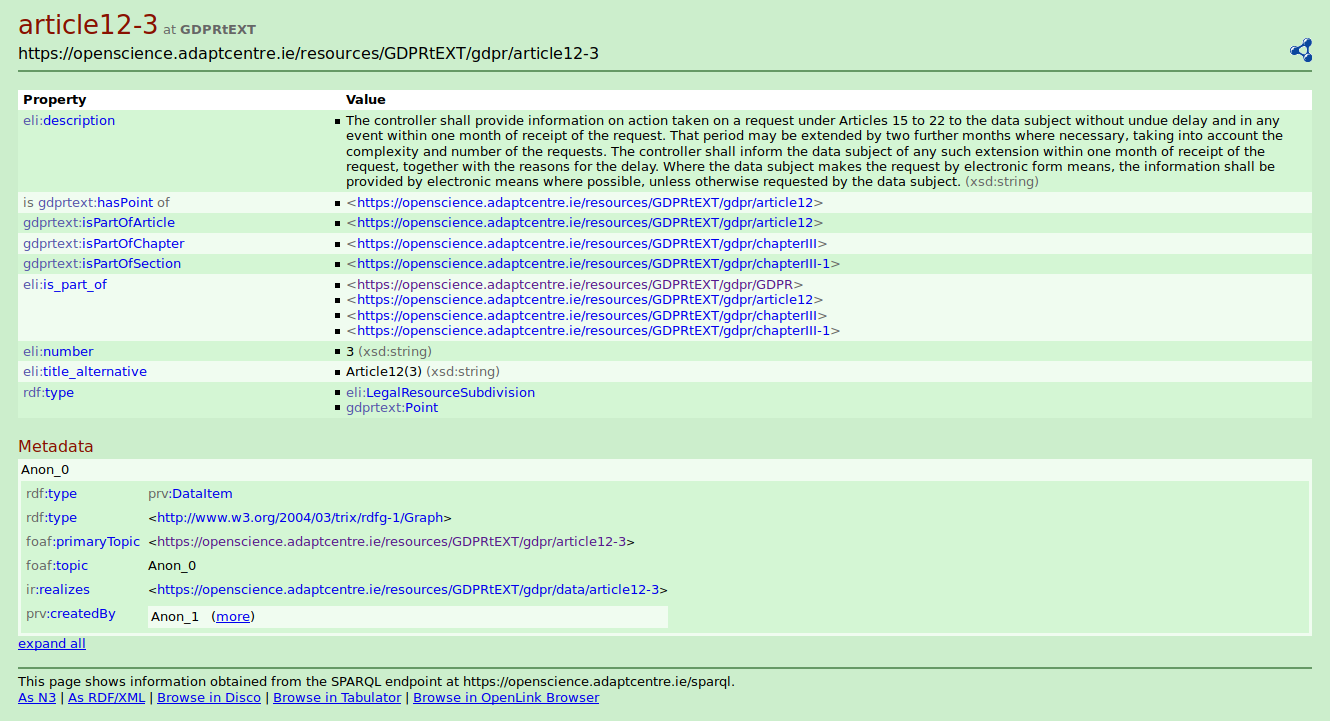
\includegraphics[width=\linewidth]{img/gdprtext-pubby}
    \caption{Article 12(3) in GDPRtEXT as RDF displayed using Pubby \cite{pandit_gdprtext_2018}}
    \label{fig:vocab:gdprtext-pubby}
\end{figure}

\subsection{Resource Description \& Application}
An visual overview of concepts within GDPRtEXT is presented in \autoref{fig:vocab:gdprtext-summary-a} and \autoref{fig:vocab:gdprtext-summary-b}.

\begin{figure}[htbp]
    \centering
    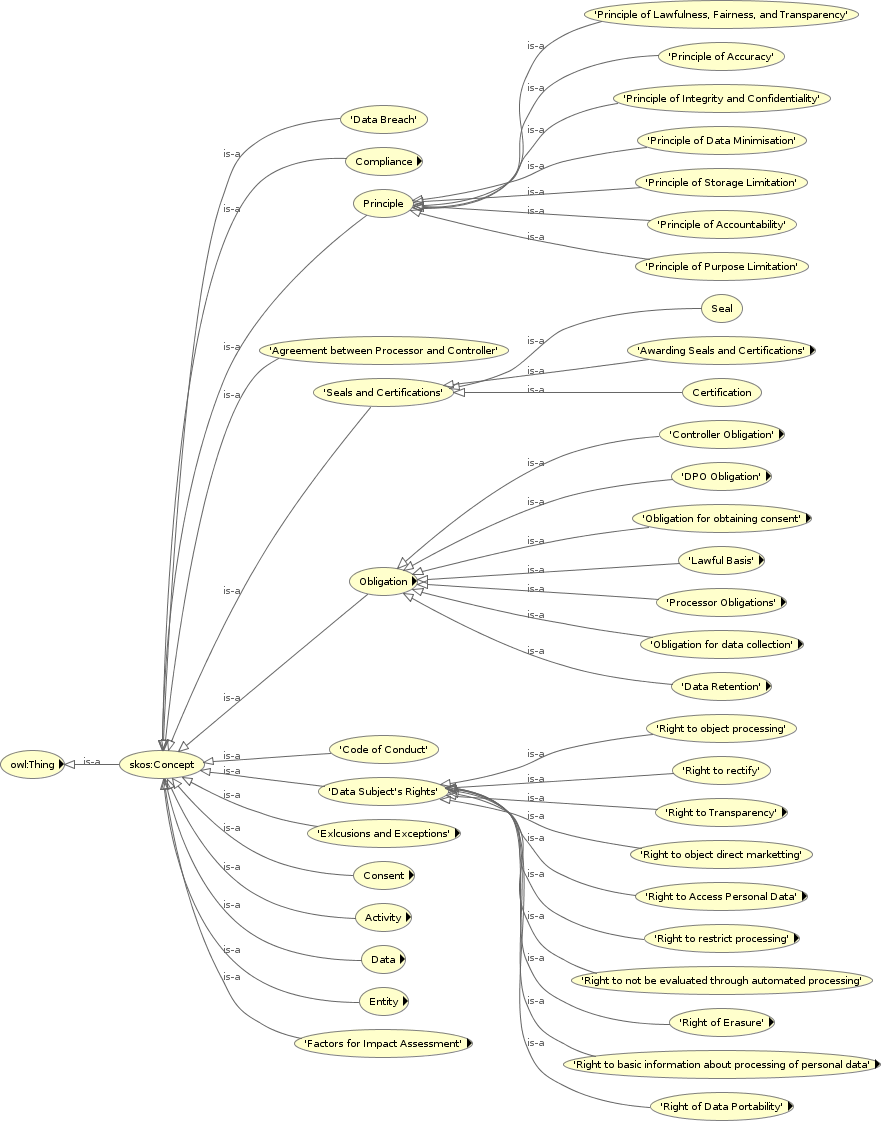
\includegraphics[width=\linewidth]{img/gdprtext-summary-a}
    \caption{Visual overview of concepts in GDPRtEXT - part (a) \cite{pandit_gdprtext_2018}}
    \label{fig:vocab:gdprtext-summary-a}
\end{figure}
\begin{figure}[htbp]
    \centering
    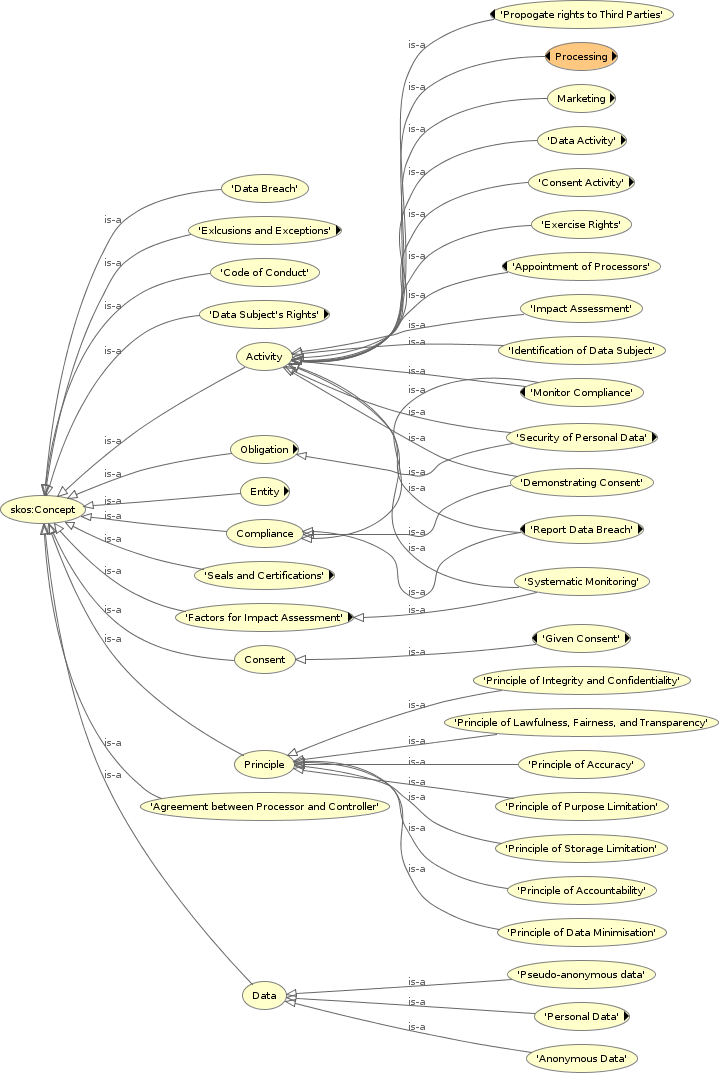
\includegraphics[width=0.75\linewidth]{img/gdprtext-summary-b}
    \caption{Visual overview of concepts in GDPRtEXT - part (b) \cite{pandit_gdprtext_2018}}
    \label{fig:vocab:gdprtext-summary-b}
\end{figure}

\subsubsection{Concepts for description structure of text}
GDPRtEXT extends European Legislation Identifier (ELI) \cite{thomas_european_2019} ontology published by European Publications Office with granular concepts to represent individual clauses within GDPR. 
ELI provides the class \texttt{LegalResource} to indicate a legislative document and its sub-class \texttt{LegalSubResource} to indicate a component or part of that resource. GDPRtEXT extends \texttt{LegalSubResource} with sub-classes \texttt{Chapter}, \texttt{Section}, \texttt{Article}, \texttt{Point} (indicating Paragraph), \texttt{SubPoint} (indicating Sub-Paragraph), \texttt{Recital}, and \texttt{Citation}.
ELI provides properties \texttt{has\_part} and its inverse \texttt{is\_part\_of} to indicate connections between two legal resources, which GDPRtEXT extends using sub-properties to indicate hierarchical relations between chapters, sections, articles, points, and sub-points.

\subsubsection{Concepts about Data}
GDPR mentions different types of data which determine applicable obligations and requirements of compliance. GDPRtEXT provides \texttt{Data} as a top-level concept to indicate abstract term of `data'.
GDPR primarily focuses on personal data as defined in Article 4(1) -  represented in GDPRtEXT as \texttt{PersonalData}, with special categories of personal data defined in Article 9(1) requiring additional obligations for processing and handling being represented by \texttt{SpecialCategoryPersonalData}. Types of special categories mentioned include criminal data, genetic data, health data, and racial data - which are defined as sub-classes in GDPRtEXT.
GDPR also mentions data in context of anonymisation and pseudo-anonymisation processes - represented in GDPRtEXT as \texttt{AnonymousData} and \texttt{PseudoAnonymousData}.

\subsubsection{Concepts about Consent}
The top-level concept of `consent' is represented by \texttt{Consent} in GDPRtEXT with its definitions based in Articles 4(11), 6(1) and Recitals 32, 40. It is sub-classed as \texttt{GivenConsent} - which is a legal basis and therefore is also a sub-class of \texttt{LegalBasis}. \texttt{GivenConsent} is further sub-classed to indicate `valid consent' which carries obligations of ensuring consent is valid and meets requirements of GDPR - and is therefore also defined as sub-class of \texttt{ObligationForObtainingConsent}. Obligations regarding conditions of valid consent are represented by sub-classing the \texttt{ValidConsent} for indicating - freely given, informed, specific, voluntary, and opt-in.

\subsubsection{Concepts about Entities}
\texttt{Entity} represents an `entity' which could be an individual, institution, company, corporation, partnership, or government agency - to name a few. 
It is sub-classed to indicate entities specifically mentioned in GDPR: Data Subject, Controller, Processor, Sub-Processor, Data Protection Officer (DPO), and Data Protection Authority (DPA). Additionally, relevant concepts associated with entities are also defined:  Representative of Controller, Representative of Processor, Certification Body, and Regulatory Authority.

\subsubsection{Concepts about Activities}
`Activity' refers to some process or action mentioned, referred, implied, or defined by requirements of GDPR compliance. To represent these, GDPRtEXT defines activities regarding consent and personal data processing, as well as other activities related to functioning of GDPR - such as reporting data breach and demonstrating consent. The top-level concept `Activity' represents abstraction of all activities. `ConsentActivity' and `DataActivity' represent specialised activities involving consent and personal data respectively.

Consent activities defined within GDPRtEXT consist of obtaining consent and withdrawing consent. Data activities include use, archival, collection, cross-border transfer, erasure, copying, rectifying, sharing, and storage of personal data. In these, the activity associated with usage of personal data is equivalent to its common and synonymous usage with term `processing'. Activities for indicating context of processing include - automated processing,  automated decision making with significant effects, confirming or matching datasets, large scale processing, processing affected or vulnerable individuals, processing sensitive data, processing using untested technologies, and unlawful processing.

GDPRtEXT also provides activities associated with reporting of data breach, which includes obligations and actions such as - report data breach, maintain record of breach, notify data subject of breach, report breach to controller (for processors), and report breach to DPA within 72 hours. Other activities provided are - security of personal data, appointment of processors, demonstrating consent, exercise rights, identification of data subject, impact assessment, marketing, direct marketing, monitor compliance, propagate rights to third parties, and systematic monitoring.

\subsubsection{Concepts about Compliance}
Concepts associated with compliance are provided to indicate actions or terms used in process of maintaining, documenting, evaluating, and demonstrating compliance. The top-level concept \texttt{Compliance} represents an abstract notion of compliance. Other terms derived from this include - Demonstration of Consent, Monitor Compliance, and Report Data Breach.

\subsubsection{Concepts about Principles}
GDPRtEXT represents principles using top-level concept \texttt{Principle}, which is specialised to indicate principles associated with: Accountability; Accuracy; Data Minimisation; Integrity and Confidentiality; Lawfulness, Fairness, and Transparency; Purpose Limitation; and Storage Limitation.

\subsubsection{Concepts about Rights}
To represent rights, GDPRtEXT provides top-level concepts representing each individual right with further concepts associated each right represented as sub-classes. 
The right of data portability is represented by \texttt{RightOfDataPortability} with related concepts regarding: providing copy of personal data, commonly used data format, machine readable format, structured, and supporting reuse.

The right of erasure is represented by \texttt{RightOfErasure} with related concepts provided regarding obligation to erase data when consent is withdrawn, or when data is no longer needed for original purpose. The right to access personal data is represented by concept \texttt{RightToAccessPersonalData} with related concepts for indicating if and where controller is processing data, whether there is automated processing with significant effects on data subject, categories of data being processed, categories of recipients data is shared with, existence of rights, information about processing, source of data, storage period, and ensuring no charges are levied for provision of rights.

\texttt{RightToBasicInformationAboutProcessing} represents right to basic information about processing and is accompanied with its related concept regarding information about third parties. The concept \texttt{RightToRestrictProcessing} represents right to restrict processing, and is accompanied with conditions such as - accuracy is contested, data no longer needed for original purpose, and processing is unlawful. The right to transparency is represented by \texttt{RightToTransparency} with related concepts regarding conditions of concise, easily accessible, intelligible, and transparent. Other represented rights include: right to not be evaluated through automated processing, right to object to direct marketing, right to object to processing, and right of rectification.

\subsubsection{Concepts about Obligations}
GDPRtEXT defines concepts regarding obligations of controllers, processors, DPOs, consent, and compliant processing of personal data based on a legal basis. Obligations of controllers are represented by \texttt{ControllerObligation} with related concepts provided regarding  appointment of processors, accountability, controller responsibility, co-operation with DPA, data protection by design and default, data security, liability of joint controller(s), maintaining records of processing activities, privacy by design, propagate rights to third parties, and reporting data breach.

Rights of processors is represented by \texttt{ProcessorObligaion} with related concepts for appointing sub-processors, assisting in complying with rights, compliance with controller's instructions, co-operating with DPA, data security, imposing confidentiality on personnel, informing controller of conflict with law, maintaining records of processing activities, only acting on documented instructions, propagating rights to third parties, providing controller with information for compliance, reporting data breach to controller, restrictions on cross-border transfers, and to return or destroy personal data at end of term.

The concept \texttt{DPOObligation} represents obligations of a DPO which include the monitoring of compliance represented by \texttt{MonitoringCompliance} . The obligations related to lawful basis for processing are represented by \texttt{LawfulBasisForProcessing} along with related concepts for contract with data subject, exempted by national law, employment law, given consent, historic, statistical, or scientific purposes, legal claims, legal obligation, legitimate interest, made public by data subject, medical or diagnostics use, not for profit organisation, public interest, purpose of new processing, and vital interest.

Obligations regarding valid consent are represented by \texttt{ValidConsent} with related concepts provided to indicate consent should be freely given, informed, specific, voluntary, and opt-in. 
Obligations for obtaining consent are represented by \texttt{ObligationForObtainingConsent} and include concepts for information about third parties, indicating consent can be withdrawn easily, and conditions regarding information provided for obtaining consent such as - it should be clear, providing explanation of processing, should not be from silence or inactivity, should be demonstrable, should be distinguishable from other matters, and that it should produce valid consent.

Obligations for data collection are represented by \texttt{ObligationForDataCollection}, which is accompanied with related concepts for indicating accurate collection, specification of explicit purpose, ensuring legitimate purpose, ensuring it is not further processed than original purpose, and ensuring it is limited to specified purpose.
Obligations for retention of personal data are represented by \texttt{ObligationForRetentionOfPersonalData} and include related concepts about    retention of personal data, ensuring it is adequate for processing, ensuring it is identifiable for required processing, obligation to kept it up to date, ensuring it is limited for processing, obligation to rectify inaccuracies, and ensuring it is relevant for processing. 
The concept \texttt{ObligationForSecurityOfPersonalData} represents obligations regarding security of personal data with related concepts provided regarding accidental loss, damage, destruction, and unlawful processing.

\subsubsection{Concepts about Seals and Certifications}
GDPRtEXT provides concepts of \texttt{Seal} and \texttt{Certification} for representing seals and certifications as provided by GDPR to assist with maintenance and demonstration of compliance.
The conditions of these are represented by \texttt{ConditionsForSealsAndCertifications}, which is further expanded to represent conditions for seal/certification such as having a maximum validity of 3 years and having a voluntary system of accreditation. 

\subsubsection{Example Use-Case: Compliance Reporting}
This example use-case, taken from documentation of GDPRtEXT \cite{pandit_gdprtext_2018}, shows how references to GDPR can aid in creation of reports which document information regarding compliance. 

Consider a system for creation of compliance reports that stores information related to obligations it addresses from GDPR. It uses the EARL\footnote{\url{https://www.w3.org/TR/EARL10-Schema/}} vocabulary for expressing results of conformance checks within the report. GDPRtEXT is used to link resources in EARL reports with articles and points within GDPR and to express and define concepts related to compliance in a suitable and comprehensible manner. Through this, information about compliance checks is linked and associated with specific articles of GDPR.

EARL provides a standardised vocabulary to describe specific resources and relationships that are relevant to test reporting. The core construct of EARL is an \texttt{Assertion}, which describes context and outcome of an individual test execution. It uses following concepts (copied verbatim from EARL specification):

\begin{itemize}
    \item \texttt{Assertor} - This can include information about who or what ran the test. For example human evaluators, automated accessibility checkers, or combinations of these.
    \item \texttt{Test Subject} - This can include web content (such as web pages, videos, applets, etc.), software (such as authoring tools, user agents, etc.), or other things being tested.
    \item \texttt{Test Criterion} - What are we evaluating test subject against? This could be a specification, a set of guidelines, a test from a test suite, or some other testable statement.
    \item \texttt{Test Result} - What was the outcome of test? A test result could also include contextual information such as error messages or relevant locations.
\end{itemize}

Taking the example of Right to Data Portability, the EARL report in \autoref{code:voc:gdprtext-earl} represents compliance checks for conditions associated with linked articles in GDPR (Article 20). The compliance system has a module \texttt{\_system\_dataportability} that checks software that handles provision of copy of personal data \texttt{\_org\_dataportability} through test case \texttt{\_test\_provide\_data\_copy} and generates a report showing the test has passed through \texttt{\_result\_pass}.


\begin{listing}
\begin{minted}{turtle}
@prefix earl: http://www.w3.org/ns/earl# .
@prefix dct:  http://purl.org/dc/terms/ .
@prefix gdprtext: http://purl.org/adaptcentre/resources/GDPRtEXT# .

_org_dataportability
    a    earl:TestSubject, earl:Software ;
    dct:description "System that handles data portability requests"@en ;
    dct:title "Data Portability Handler"@en .

_system_dataportability
    a    earl:Assertor ;
    dct:description "Module checking data portability obligations"@en ;
    dct:hasVersion "1.4" ;
    dct:title "DataPortability Module"@en ;
    earl:asserts { 
      _org_dataportability _result_pass _test_provide_data_copy } .

_result_pass
    a    earl:ResultProperty ;
    earl:date "2018-01-01" ;
    earl:validity earl:Pass ;
    earl:confidence earl:High .

_test_provide_data_copy
    a    earl:TestCase ;
    earl:testMode earl:automatic ;
    dct:title "Test provision of data copy"@en ;
    dct:description "Tests whether system provides a copy 
      of personal data on exercising right to data portability"@en ;
    dct:subject gdprtext:article20 .
\end{minted}
\label{code:voc:gdprtext-earl}
\caption{Use of GDPRtEXT to link tests with GDPR Articles in EARL report}
\end{listing}

To gather related resources together, a SPARQL query (simplified) would focus on link between \texttt{TestCase} and its result using \texttt{earl:validity}, as shown in \autoref{code:voc:gdprtext-sparql}.
These tests can be further combined into test suites to group compliance checks related to each article or a particular concept and structure  documentation around this form of logical grouping of concepts.
In this manner, use of GDPRtEXT to link tests and results with documentation enables automation of information retrieval and management.
A similar use-case of GDPRtEXT in linking constraints and their outcomes with GDPR is demonstrated in \autoref{chapter:testing}.

\begin{listing}
\begin{minted}{sparql}
SELECT ?gdpr ?result ?confidence ?mode WHERE {
    ?assertor a earl:Assertor .
    ?assertor earl:asserts ?assertion .

    ?testcase rdf:predicate ?assertion .
    ?testcase a earl:TestCase .
    ?testcase dct:subject ?gdpr .
    ?testcase ear:testMode ?mode .

    ?testresult rdf:object ?assertion .
    ?testresult a earl:ResultProperty .
    ?testresult earl:validity ?result .
    ?testresult earl:confidence ?confidence .
}

| gdpr          | result     | confidence     | mode          |
---------------------------------------------------------------
| article16     | pass       | low            | automatic     |
| article17     | pass       | high           | automatic     |
| article18     | fail       | high           | manual        |
| article19     | pass       | high           | automatic     |
\end{minted}
\label{code:voc:gdprtext-sparql}
\caption{SPARQL query and results showing retrieved GDPR test results by article}
\end{listing}

\subsubsection{Example Use-Case: Mapping between DPD and GDPR obligations}
The second application of GDPRtEXT, taken from its publication \cite{pandit_gdprtext_2018}, demonstrates linking of obligations between GDPR and its predecessor - Data Protection Directive (DPD. Given that DPD was adopted in 1995, and was superseded by GDPR in 2016, there are a large number of solutions and approaches regarding compliance with DPD that already exist and are used in practice. By linking obligations between DPD and GDPR it is possible to investigate reuse of these existing solutions for GDPR compliance. To that end, a mapping from DPD obligations to GDPR obligations containing annotations that describe nature of changes is constructed by linking articles of DPD and GDPR.

To model annotations as a RDF resource, a linked data version of DPD was created similar to GDPRtEXT by assigning URIs for every clause in legislation. This enabled referring to each individual clause in DPD and linking it with relevant clauses in GDPR. 
The annotations (available online\footnote{\url{https://openscience.adaptcentre.ie/projects/GDPRtEXT/dpd_mapping.html}}) consist of references from a clause in DPD to its corresponding clause in GDPR with an expression of change between the two. The nature of change is represented by values: same - indicating no change; reduced - indicating reduction of obligation; slightly changed - indicating minor change; completely changed - indicating major change; and extended - indicating addition of obligations.

Its example demonstration consisted of using XACML\footnote{\url{https://www.oasis-open.org/committees/tc_home.php?wg_abbrev=xacml}} rules for controlling access to data and modelled after DPD obligations.
For each link between DPD and GDPR obligations, a record was created indicating whether the corresponding XACML rules for DPD compliance needed to be changed to be applicable for GDPR. The notation \texttt{N/A} was used to denote cases where no XACML rules existed for a particular DPD obligation and where corresponding obligations in GDPR had changed or had additional requirements. 
\begin{listing}[htbp]
\begin{minted}{turtle}
@prefix gdpr: https://w3id.org/GDPRtEXT/gdpr# .
@prefix dpd: https://w3id.org/GDPRtEXT/dpd# .
@prefix rdfs: http://www.w3.org/2000/01/rdf-schema# .

dpd:mappingrule6
    a dpd:DPDToGDPR_Annotation ;
    dpd:hasChange dpd:ChangeExtended ;
    dpd:hasXACMLChange dpd:XACMLNoChange ;
    dpd:resourceInDPD dpd:Article7 - a ;
    dpd:resourceInGDPR gdpr:Article6-1-a ;
    rdfs:comment "added consent given to ..." .
\end{minted}
\label{code:voc:gdprtext-xacml}
\caption{Example annotation of associating existing DPD compliance XACML rules with requirements of GDPR}
\end{listing}
% The value \texttt{No} was used to indicate no changes in the GDPR obligation compared to the DPD obligation, so that the existing XACML rule would be sufficient to meet GDPR requirements. Similarly \texttt{Yes} was used to indicate a change required in the XACML rule to handle the obligation.

The class \texttt{DPDToGDPR\_Annotation} represents annotations between DPD and GDPR, with an example instance depicted in \autoref{code:voc:gdprtext-xacml}. The property \texttt{resourceInDPD} is used to refer to a specific clause within DPD using its IRI. Similarly, the property \texttt{resourceInGDPR} is used to refer to a corresponding clause in GDPR. The nature of change is defined using property \texttt{hasChange} whose value is an instance of class \texttt{ChangeInObligation}, with instances defined for \textit{Extended, Same, Reduced, CompletelyChanged}, and \textit{SlightlyChanged}. Similarly, a change in XACML rules is defined using class \texttt{ChangeInXACMLRule} with instances \textit{Yes, No}, and \textit{N/A}.

\subsection{Evaluation}\label{sec:voc:gdprtext:evaluation}
In terms of ontology assessment, the methodology outlined in \autoref{sec:voc:methodology} provides criterion for evaluation of ontology quality and documentation. GDPRtEXT fulfils these based on using OOPS! tool\footnote{OOPS! results published with ontology documentation. The results can also be independently obtained using the OOPS! online service.} to identify and rectify bad design patterns and by following best practices and community guidelines for ontology documentation.
GDPRtEXT and the work described in this section was published \cite{pandit_gdprtext_2018} at Extended Semantic Web Conference (ESWC) - Resource Track. The publication described creation of resource, summarised its contents, and described mapping of DPD obligations with GDPR using a linked data approach and XACML to denote which obligations from DPD could be re-used towards GDPR compliance. 
ESWC is a premier and top-tier conference within semantic web domain, and has a rigorous review process with an open review policy.
The acceptance of GDPRtEXT in this venue demonstrates its value as a semantic web resource.

To date, the publication has received 19 citations from peer-reviewed publications (excluding self-citations) on Google Scholar\footnote{\url{https://scholar.google.com/scholar?cites=2776106745007214232}}.
In addition to these, a 5 star rating given to GDPRtEXT as a dataset in Irish open data portal indicates its adherence to linked data principles.
% The publications associated with PrOnto \cite{palmirani_pronto_2018,palmirani_pronto_2018-1} cite GDPRtEXT as a resource of GDPR concepts and comment on  modelling of the norms and the legal axioms - which are not within the scope of GDPRtEXT or this thesis. It also mentions the lack of FRBR
% \footnote{Functional Requirements for Bibliographic Records (FRBR) is a conceptual entity–relationship model which allows expressing legal text as an abstract document with expressions in different languages and manifestations in different representations. It was adopted for use in ELI in the legislation passed on 6 November 2017 (OJ C 441, 22.12.2017, p. 8–12 \url{https://eur-lex.europa.eu/legal-content/EN/TXT/?uri=CELEX:52017XG1222(02)}).}
% information for managing versioning of the legal text over the time.
% However, it must be noted that since the ELI ontology itself uses FRBR and that GDPRtEXT extends ELI, it is capable of supporting the FRBR concepts as well - but does not provide them since the aim of the work is to enable granular references to its clauses rather than a provision of its text in multiple languages and representations. 
A survey of legal approaches within state of the art \cite{leone_taking_2019} undertaken by MIREL project analysed GDPRtEXT amongst other legal ontologies and found that GDPRtEXT is singular in its use of ELI and provision of GDPR as a glossary of concepts - a finding shared with the analyses of SotA in \autoref{sec:sota:analysis}.

\subsubsection{Fulfilment of Competency Questions}
The assessment of GDPRtEXT consists of evaluating the extent to which it answers competency questions outlined in \autoref{sec:voc:gdprtext-engineering}.
For this, \autoref{table:gdprtext:eval-cq} shows concepts and relationships of GDPRtEXT relevant towards answering competency questions.
\begin{table}[htbp]
\footnotesize
\centering
\rowcolors{1}{}{gray!10}
\begin{tabularx}{\textwidth}{|l|X|}
\caption{Concepts in GDPRtEXT for answering competency questions} \\ \hline
\label{table:gdprtext:eval-cq}
\textbf{CQ} & \textbf{Concepts/Relationships} \\ \hline
% & \textbf{Concepts associated with structure of GDPR} \\ \hline
\textit{CQ1-7} & \textit{Recital, Chapter, Section, Article, Point, SubPoint, Reference, Citation} \\ \hline
% \textit{CQ2} & \textit{Chapter} \\ \hline
% \textit{CQ3} & \textit{Section} \\ \hline
% \textit{CQ4} & \textit{Article} \\ \hline
% \textit{CQ5} & \textit{Point} \\ \hline
% \textit{CQ6} & \textit{SubPoint} \\ \hline
% \textit{CQ7} & \textit{Reference}, \textit{Citation} \\ \hline
\textit{CQ8} & \textit{isPartOfChapter} \\ \hline
\textit{CQ9,11} & \textit{rdfs:isDefinedBy [Article, Point, SubPoint]} \\ \hline
\textit{CQ10} & \textit{:\_ hasPart/isPartOf :\_} \\ \hline
% \textit{CQ11} & \textit{Accountability} \\ \hline
\textit{CQ12} & \textit{:GivenConsent rdfs:seeAlso [Article, Point, SubPoint]} \\ \hline
% \textit{CQ13} & \textit{GivenConsent} \\ \hline
\textit{CQ13,14} & \textit{GivenConsent/Compliance :involves [Article, Point, SubPoint]} \\ \hline

% & \textbf{Concepts associated with GDPR compliance} \\ \hline
\textit{CQ15} & \textit{Data}, \textit{PersonalData}, \textit{SensitivePersonalData}, \textit{CriminalData}, \textit{GeneticData}, \textit{HealthData}, \textit{RacialData}, \textit{AnonymousData}, \textit{PseudoAnonymousData} \\ \hline
\textit{CQ16} & \textit{Consent}, \textit{GivenConsent}, \textit{WithdrawnConsent} \\ \hline
\textit{CQ17} & \textit{Entity}, \textit{DataSubject}, \textit{Controller}, \textit{JointController}, \textit{Processor}, \textit{SubProcessor}, \textit{DPO}, \textit{DPA}, \textit{ControllerRepresentative}, \textit{ProcessorRepresentative}, \textit{CertificationBody}, \textit{RegulatoryAuthority} \\ \hline
\textit{CQ18,19} & \textit{DataActivity, ConsentActivity} \\ \hline
% \textit{CQ19} & \textit{ConsentActivity} \\ \hline
\textit{CQ20} & \textit{Processing}, \textit{AutomatedProcessing}, \textit{AutomatedDecisionMakingWithSignificantEffect}, \textit{ConfirmingOrMatchingDatasets}, \textit{LargeScaleProcessing}, \textit{ProcessingAffectedOrVulnerableIndividuals}, \textit{ProcessingSensitiveData}, \textit{ProcessingUsingUntestedTechnologies}, \textit{Unlawful} \textit{Processing} \\ \hline
\textit{CQ21} & \textit{ReportDataBreach}, \textit{MaintainRecordOfBreach},  \textit{NotifyDataSubjectOfBreach}, \textit{ReportBreachToController}, \textit{ReportBreachToDPAWithin72Hours} \\ \hline
\textit{CQ22} & \textit{Compliance}, \textit{Demonstration}, \textit{ConsentMonitor}, \textit{Compliance}, \textit{ReportDataBreach}  \\ \hline
\textit{CQ23} & \textit{Principle}, \textit{Accountability}, \textit{Accuracy}, \textit{DataMinimisation}, \textit{IntegrityAndConfidentiality}, \textit{LawfulnessFairnessAndTransparency}, \textit{PurposeLimitation}, \textit{StorageLimitation}  \\ \hline
\textit{CQ24} & \textit{Rights}, \textit{RightOfDataPortability}, \textit{RightOfErasure}, \textit{RightToAccessPersonalData}, \textit{RightToTransparency}, \textit{RightToBasicInformationAboutProcessing}, \textit{RightToNotBeEvaluatedThroughAutomatedProcessing}, \textit{RightToObjectForDirectMarketting}, \textit{RightToObjectToProcessing}, \textit{RightToRectify}, \textit{RightToRestrictProcessing} \\ \hline
\textit{CQ25} & \textit{RightOfDataPortability}, \textit{ProvideCopyOfPersonalData}, \textit{ShouldBeCommonlyUsedFormat}, \textit{ShouldBeMachineReadable}, \textit{ShouldBeStructured}, \textit{ShouldSupportReuse}  \\ \hline
\textit{CQ26} & \textit{RightToBasicInformationAboutProcessing}, \textit{InformationAboutThirdParties}  \\ \hline
% \textit{CQ27} & \textit{Obligation} \\ \hline
\textit{CQ27,28} & \textit{Obligation, ControllerObligation}, \textit{AppointmentOfProcessors}, \textit{Accountability}, \textit{ControllerResponsibility}, \textit{CooperateWithDPA}, \textit{DataProtectionByDesignAndDefault}, \textit{DataSecurityLiabilityOfJointControllers}, \textit{MaintainRecordsOfProcessingActivities}, \textit{PrivacyByDesign}, \textit{PropogateRightsToThirdParties}, \textit{ReportDataBreach} \\ \hline
\textit{CQ29} & \textit{ProcessorObligation}, \textit{AppointingSubprocessors}, \textit{AssistInComplyingWithRights}, \textit{ComplianceWithControllersInstructions}, \textit{CooperateWithDpa}, \textit{DataSecurity}, \textit{ImposeConfidentialityOnPersonnel}, \textit{InformControllerOfConflictWithLaw}, \textit{MaintainRecordsOfProcessingActivities}, \textit{OnlyActOnDocumentedInstructions}, \textit{PropogateRightsToThirdParties}, \textit{ProvideControllerWithInformationForCompliance}, \textit{ReportDataBreachToController}, \textit{RestrictionsOnCross}-\textit{borderTransfers}, \textit{ReturnOrDestroyPersonalDataAtEndTerm} \\ \hline
\textit{CQ30} & \textit{DPOObligation}, \textit{MonitorCompliance} \\ \hline
\textit{CQ31} & \textit{LawfulBasisForProcessing}, \textit{ContractWithDataSubject}, \textit{ExemptedByNationalLaw}, \textit{EmploymentLaw}, \textit{GivenConsent}, \textit{HistoricStatisticalOrScientificPurposes}, \textit{LegalClaims}, \textit{LegalObligation}, \textit{LegitimateInterest}, \textit{MadePublicByDataSubject}, \textit{MedicalDiagnosticOrTreatement}, \textit{NotForProfitOrg}, \textit{PublicInterest}, \textit{PurposeOfNewProcessing}, \textit{VitalInterest} \\ \hline
\textit{CQ32} & \textit{ValidConsent}, \textit{FreelyGivenConsentObligation}, \textit{InformedConsentObligation}, \textit{SpecificConsentObligation}, \textit{VoluntaryOptInConsentObligation}  \\ \hline
\textit{CQ33} & \textit{ObligationForDataCollection}, \textit{AccurateCollection}, \textit{ExplicitPurpose}, \textit{LegitimatePurpose}, \textit{NotFurtherProcessedThanOriginalPurpose}, \textit{SpecifiedPurpose} \\ \hline
\textit{CQ34} & \textit{InformationAboutThirdParties}, \textit{ConsentCanBeWithdrawnEasily}, \textit{ClearExplanatinOfProcessing}, \textit{NotFromSilenceOrInactivity}, \textit{Demonstrable}, \textit{DistinguishableFromOtherMatters}, \textit{ValidConsent} \\ \hline
\textit{CQ35} & \textit{RetentionOfPersonalData}, \textit{AdequateForProcessing}, \textit{IdentifiableForRequiredProcessing}, \textit{KeptUpToDate}, \textit{LimitedForProcessing}, \textit{RectifyInaccuracies}, \textit{RelevantForProcessing} \\ \hline
\textit{CQ36} & \textit{SecurityofPersonalData}, \textit{AccidentalLoss}, \textit{Damage}, \textit{Destruction}, \textit{UnlawfulProcessing} \\ \hline
\textit{CQ37} & \textit{Seal}, \textit{Certification}
\end{tabularx}
\end{table}
The table demonstrates that GDPRtEXT provides concepts to answer all  competency questions. GDPRtEXT thus meets requirements of representing and linking information with text and concepts of GDPR in a granular manner and fulfils $RO3(a)$.

\subsubsection{Comparison with SotA}
The SotA in representing text of GDPR in machine-readable formats presented in \autoref{sota:analysis:representation} compared three approaches: ELI \cite{thomas_european_2019}, Agarwal et al \cite{agarwal_legislative_2018}, and PrOnto \cite{palmirani_pronto_2018,palmirani_pronto_2018-1}.
Their comparison and analysis, summarised in \autoref{table:sota:analysis:GDPR}, depicts relevance of each approach in representing the GDPR as a glossary of concepts, providing a permanent identifier for resources, modelling of GDPR's text, and whether resources are open and accessible.
The conclusion drawn from these is the lack of an approach fulfilling all criteria along with a lack of open and reusable resources concerning GDPR. 
The additional resource of ELI+ mentioned in analysis shows intention of EU Publications Office to remedy this gap through an update to the ELI ontology at some time in future.

A comparison of GDPRtEXT with these approaches, depicted in \autoref{table:gdprtext:sota}, shows that GDPRtEXT provides a glossary of concepts, uses permanent identifiers, provides linked data version of text of GDPR, and is available under an open and permissive license (CC-BY-4.0).
This matches the intended contributions of ELI+ (update to ELI) planned by EU Publications Office, and therefore enables GDPRtEXT to fill this gap in this time.

\begin{table}[htbp]
\footnotesize
\centering
\caption{Comparison of GDPRtEXT with SotA}\label{table:gdprtext:sota}
\rowcolors{1}{}{gray!10}
\begin{tabular}{|l|>{\columncolor[gray]{0.9}}l|l|l|l|l|}
\hline
Work & \textbf{GDPRtEXT} & ELI & ELI+ & Agarwal et al & PrOnto \\ \hline
Vocabulary & ELI & OWL2 & OWL2 & RDFS & Akoma Ntoso \\ \hline
Granularity & Sub-Paragraph & Legislation & Sub-Paragraph & Paragraph & Sub-Paragraph \\ \hline
Glossary & \cmark & \xmark & \cmark & \xmark & \xmark \\ \hline
PID & \cmark & \cmark & \cmark & \xmark & \xmark \\ \hline
OA & \cmark & \cmark & \cmark & \xmark & \xmark \\ \hline
GDPR text & \cmark & \xmark & \cmark & \xmark & \cmark \\ \hline
\end{tabular}
\end{table}

A survey of legal ontologies by Leone et al. \cite{leone_taking_2019} includes GDPRtEXT as an ontology relevant for data protection. The survey also includes ELI and PrOnto within the scope of data protection ontologies - which provides external comparison between these and GDPRtEXT. The survey outlines the role of GDPRtEXT in acting as a glossary of concepts rather than a prescriptive set of norms and rules for specification of compliance - such as made available through PrOnto. In this role, GDPRtEXT is novel within state of the art given a lack of other similar resources.

Based on this, GDPRtEXT is argued to provide novel contribution to state of the art and addresses gaps associated with representation of concepts and GDPR text at a granular level, and whose open availability enables usage and adoption.

\subsection*{Summary}
The GDPRtEXT resource represents the first major contribution of this thesis. It provides a linked data version of text of GDPR and a glossary of its concepts, fulfils research objective $RO3(a)$, and assists with research objective $RO5(b)$ - as outlined in \autoref{sec:intro:RQ}. It enables representing each article or point within GDPR as a unique resource through IRIs defined using RDF and semantic web.
GDPRtEXT thus enables machine-readable links to be established between information and clauses of GDPR as well as concepts pertaining to its compliance.

The use of GDPRtEXT makes it possible to create approaches that automate generation and querying of information associated with GDPR - such as for compliance, management of business processes, or generation of privacy policies. The compatibility provided through extension of ELI ontology ensures alignment with official documents produced by European Publications Office.
Finally, GDPRtEXT fills an important gap in the state of the art regarding machine-readable approaches for linking information with legal text.
GDPRtEXT has been released as an open resource, has been published in Zenodo and Datahub, and has been incorporated into Ireland’s open data portal as a 5-star linked open dataset.

% GDPRov
\section{GDPRov - Ontology for GDPR activities associated with Personal Data and Consent}\label{sec:voc:GDPRov}
This section describes the GDPRov ontology for representing activities in ex-ante and ex-post phases associated with processing of personal data and consent for GDPR compliance. GDPRov stands for GDPR Provenance - a reference to the requirement of maintaining provenance information of processes in both ex-ante and ex-post phases for demonstrating GDPR compliance. This section presents motivation, overview, dissemination, and evaluation of GDPRov ontology. It also presents comparisons with relevant approaches in state of the art. 

The ontology satisfies the research objectives $RO3(b)$ presented in \autoref{sec:intro:RQ}.
It uses the compliance questions presented in \autoref{sec:info:compliance-questions} as competency questions to identify requirements and for evaluation.
GDPRtEXT is used to define and associate the source of concepts within the text of GDPR.
An earlier version (v0.4) of GDPRov was described in a peer-reviewed publication \cite{pandit_modelling_2017}.
Subsequent revisions included addition of new concepts associated with real-world implementation and interpretation of GDPR compliance requirements (see \autoref{sec:testing:sparql}) and for representing information about consent mechanisms on the internet (see \autoref{sec:testing:shacl}).
The latest version of GDPRov (v0.7) is available online\footnote{\url{http://w3id.org/GDPRov}} with its documentation and code repository\footnote{\url{https://github.com/coolharsh55/GDPRov}}.

\subsection{Identification of requirements from competency questions}\label{sec:gdprov:cq}
The compliance questions presented in \autoref{sec:info:compliance-questions} were selected based on relevance to information regarding activities and provided competency questions for deriving concepts and relationships regarding processes associated with personal data and consent in the context of GDPR compliance requirements. 
These concepts and relationships were collected, combined, and analysed to ensure their cohesion as an ontology and evaluated against the compliance questions to ensure they satisfied requirements regarding GDPR compliance and documentation of associated processes.
In this, the aspect of ex-ante and ex-post processes provides a form of duplication as most processes have their counterparts in both phases, and which is linked and documented in a manner so as to demonstrate the prior planning of processes to ensure their compliance and their execution - which both need to be documented to demonstrate compliance.
Therefore, while GDPR requirements and the compliance questions do no explicitly mention the existence of ex-ante and ex-post phases for each activity, the development of GDPRov explicitly considers each activity to have representations in both phases.

The sub-sections below present the concepts arising from competency questions. 
This is followed by an analysis of discovered concepts in ex-ante and ex-post phases.
The analysis leads to requirements towards the construction of the GDPRov ontology, and serves to describe the motivation behind its design and implementation.

\subsubsection{Actors and Agents involved in activities}
\begin{itemize} 
    \item \texttt{CMQ2} - Provides the concept of \textit{Controller} as an agent controlling the processes as defined by and its representative \textit{Data Protection Officer (DPO)}.
    \item \texttt{CMQ17} - Describes the \textit{Processor} as an executor of processes and its representative \textit{DPO}. In this relationship, the \textit{Controller} provides such processes to the \textit{Processor} to execute, which is governed by a \textit{Data Processing Agreement (DPA)} between the two.
    \item \texttt{CMQ35} - Describes \textit{Data Subject} as an agent who is associated with the provision of personal data, consent, and who is related to the exercising of rights.
\end{itemize}

\subsubsection{Details of processing}
\begin{itemize}
    \item \texttt{CMQ3} and \texttt{CMQ37} provide the concept of \textit{Purpose} which describes the purpose of personal data processing. Each purpose can incorporate multiple processing operations, and each processing operation taking place can be associated with multiple purposes.
    \item \texttt{CMQ4} describe the necessity to specify data subject categories whose personal data is being processed.
    \item \texttt{CMQ36} describes personal data, while \texttt{CMQ5} describes categories of personal data being processed. \texttt{CMQ34} specifies special categories of personal data as a sub-category of personal data which needs to be explicitly stated as being processed.
    \item \texttt{CMQ38} defines processing of personal data as defined by Article 4-2 of GDPR. The GDPR definition of processing provides types of operations considered under processing, as specified by ``\textit{any operation or set of operations which is performed on personal data or on sets of personal data, whether or not by automated means, such as collection, recording, organisation, structuring, storage, adaptation or alteration, retrieval, consultation, use, disclosure by transmission, dissemination or otherwise making available, alignment or combination, restriction, erasure or destruction;}''.
    \item \texttt{CMQ6} defines sharing of data as a type of processing. Additional information associated with sharing of data is provided by - \texttt{CMQ7} and \texttt{CMQ20} for categories of recipients; \texttt{CMQ8},\texttt{CMQ21} for identifies of recipients, \texttt{CMQ9} and \texttt{CMQ22} for location where data is being sharing to; \texttt{CMQ10} and \texttt{CMQ23} for safeguards associated with data transfer; \texttt{CMQ15} and \texttt{CMQ25} for purposes of sharing, which is the same concept as purpose of processing except applied for sharing of personal data.
    \item \texttt{CMQ11} defines data storage, with additional concepts provided by \texttt{CMQ12} for existence of time limits or conditions for erasure and \texttt{CMQ13} for specification of time limits or conditions for erasure for categories of data.
    \item \texttt{CMQ26} defines legal basis for justifying the processing of personal data, and \texttt{CMQ27} specifies legal basis associated with a particular purpose. Each purpose can have one or more legal basis associated with it.
\end{itemize}

\subsubsection{Life-cycle of data}
\begin{itemize}
    \item \texttt{CMQ28} and \texttt{CMQ30} describe source of personal data which in turn implies an activity that collects data and specifies the actor or agent providing the data.
    \item \texttt{CMQ29} specifically refers to personal data collected from data subject.
\end{itemize}

\subsubsection{Anonymisation}
\begin{itemize}
    \item \texttt{CMQ31} specifies anonymisation of personal data, with \texttt{CMQ32} inquiring about different `levels' of anonymisation which affect the application of obligations and requirements of compliance. 
    \item The levels are specified based on their application in the process of compliance, and include data which is completely anonymised, data which is pseudo-anonymised, and data which is not anonymised. In this, data that is pseudo-anonymised can be considered and used as anonymous data under the condition that the organisation does not have additional information to de-anonymise it. 
    \item From this, the processing associated with anonymisation and de-anonymisation of personal data are defined.
\end{itemize}

\subsubsection{Activities associated with Consent}
\begin{itemize}
    \item Regarding consent, \texttt{CMQ48} inquires about activities associated with the provision and collection of consent. This includes information about how the consent is requested and collected, used within processes as a legal basis, and is archived for future demonstration of compliance.
    \item \texttt{CMQ49} and \texttt{CMQ50} inquire about artefacts associated with the collection of consent as determination of validity of consent under GDPR require investigation of how choices for consent were offered. This also includes the form in which consent is provided or collected from the data subject. The artefacts are associated with the processes where consent choices are offered or requested and whose result is the collection of consent.
\end{itemize}

\subsubsection{Provision of Rights}
\begin{itemize}
    \item The rights associated with GDPR need processes to internally (from the perspective of the organisation) handle their execution as well as for interaction with the data subject. Therefore, such processes need to be defined and documented for compliance purposes.
    \item In the case of right to be informed, \texttt{CMQ88 - CMQ105} provide the competency questions regarding how the right is provided and how it is executed or implemented.
    \item This includes activities associated with the provision of information to the data subject, artefacts associated with information provision, inclusion of details such as controller and DPO, purposes, processing, legal basis, personal data categories.
    \item It also includes information about sources of personal data (where not obtained directly from the data subject), and whether the legal basis is legitimate interest.
    \item Regarding data sharing, the information to be specified includes categories of recipients , and their location.
    \item The right to be informed also includes provision of information regarding the existence and application of rights.
    \item The information associated with the right to be informed is common to other information documented in the due course of processing of personal data, and therefore does not specifically require separate notation or representation of this information in order to execute the right. the existing information or concepts can be reused for specifying the required information. However, activities associated with the right need to be defined to demonstrate the existence of processes for handling the right.
\end{itemize}

\subsubsection{Compliance procedures such as Reporting of Data Breach}
\begin{itemize}
    \item The reporting of data breach requires information about data breach to be maintained, as specified by \texttt{CMQ106 - CMQ120}.
    \item This includes information about the data breach, which includes timestamp of when the breach occurred (\texttt{CMQ106}), timestamp of when the controller became aware of it (\texttt{CMQ107}), timestamp and method of it being notified to supervisory authority (\texttt{CMQ108}).
    \item Information about contents of breach include information about its affected personal data and categories of data subject (\texttt{CMQ112}).
    \item This information is associated with the process of reporting and documenting data breach in the form of artefacts. This information also needs to be provided to the supervisory authority and in some cases to the data subject based on the extent of the breach (\texttt{CMQ113}) and therefore requires prior plans to execute the process and handle a data breach and send the information to data subjects along with any remedial measures (\texttt{CMQ116}).
\end{itemize}

\subsubsection{Specifying requirements for ex-ante and ex-post phases}
Process logs are a convenient and demonstrable form of information to store and document the compliant processing of personal data. By verifying such logs, it is possible to document, evaluate, and demonstrate that the executed processes were compliant with the requirements of GDPR. This constitutes as ex-post phase of compliance, and consists of evaluating information after the processing has been carried, such as for Article 30 of the GDPR concerning processing records to be maintained. Along with this, it is also essential to demonstrate that the executed processes were based on a preconceived plan or template that was ensured to be compliant before the actual execution. Storing such plans is essential to demonstrate prior planning and maintenance of a compliant processing system. This constitutes as ex-ante phase of compliance, and consists of evaluating compliance on plans of processing yet to be carried out, such as for Article 35 of the GDPR concerning carrying out a DPIA.

Associating the executed processes with their plans allows demonstration of compliance throughout the life-cycle of the process, i.e. from the planning of processes to their eventual execution. It also enables documenting change in plans and its effects on execution of processes - i.e. when a plan changes, it also brings about corresponding changes in the executed processes. In the context of GDPR compliance, the requirements of compliance require documentation, maintenance, and demonstration of processes across both ex-ante (planning) and ex-post (execution) phases. The ex-ante plans of processes are described as an organisational measure and their compliance is associated with ensuring processes meet legal requirements before they are actually carried out. In some instances, such as for a Data Protection Impact Assessment (DPIA), the existence of ex-ante information about processes is essential to the evaluation of compliance.

While the compliance questions provide a basis for identifying information to be modelled, the requirements of expressing this information in ex-ante and ex-post phase enable the specification of their intended usage in planning and processing stages respectively, which further determines whether the compliance evaluation consists of verification of a plan or analysis of processing logs. 
The requirements crafted from the above provide motivation and argument for representing processes in ex-ante and ex-post.
This represents a design decision based on separating representation of information across phases of compliance rather than a compliance requirement itself.
Approaches within the state of the art that also follow a similar representation include SPECIAL (\autoref{sec:sota:SPECIAL}) which uses PROV-O to log information in both phases, and MIREL (\autoref{sec:sota:MIREL}) which uses a workflow model to represent a plan and its executions.

The information requirements for modelling information about activities is summarised through the following points:
\begin{enumerate}
    \item Represent process in ex-post phase as a log or record.
    \item Represent process in ex-ante phase as plan or template.
    \item Link ex-ante plan with its instantiations or executions in ex-post phase.
    \item Track the provenance of ex-ante plans i.e. changes in plans of processes.
    \item Enable tracking changes in ex-post logs based on corresponding changes in ex-ante plans.
    \item Associate information used/generated in activities as artefacts in both ex-ante and ex-post phases.
    \item Associate actors/agents with processes.
    \item Link processes based on:
        \begin{enumerate}
            \item dependency - where one process is dependant on another through use of generated artefact,
            \item order of execution - where one process is or will be executed before or after another, and
            \item composition - where one process is constituted by several sub-processes.
        \end{enumerate}
\end{enumerate}

\subsection{Extending PROV-O and P-Plan}
Based on the above stated requirements for representing activities or processes in ex-ante and ex-post phases, the existing semantic web ontologies of PROV-O \cite{lebo_prov-o_2013} and P-Plan \cite{garijo_p-plan_2014} were extended with relevant GDPR concepts and relationships to create the GDPRov ontology. The necessity of this process and a brief overview of PROV-O and P-Plan ontologies is presented below along with the process of extending the two ontologies.

\subsubsection{PROV - W3C standard for representing provenance information}
Provenance is information about entities, activities, and people (or software)
involved in producing data or a component which can be used to form an
assessment about its quality, reliability, or trustworthiness. The PROV-O ontology \cite{lebo_prov-o_2013} along with PROV family\footnote{\url{https://www.w3.org/TR/2013/NOTE-prov-overview-20130430/}} of schemas and documents is the W3C recommendation since 30\textsuperscript{th} April 2013 for representing provenance information as has seen significant adoption by the semantic web and industrial community.
It provides definitions for interchange of provenance information by representing entities
and relations between them such as generated by, derived from, and attributions.

The core concepts of PROV-O are summarised in \autoref{fig:prov-o-model}, and consist of interactions between \textit{Activities}, \textit{Entities}, and \textit{Agents}.
An \texttt{Entity} in PROV-O is defined as being physical, digital, conceptual, or other
kind of thing with some fixed aspects. PROV-O defines an \texttt{Activity} as something
that occurs over a period of time and acts upon or with entities; it may include
consuming, processing, transforming, modifying, relocating, using, or generating
entities.
\begin{figure}[htbp]
    \centering
    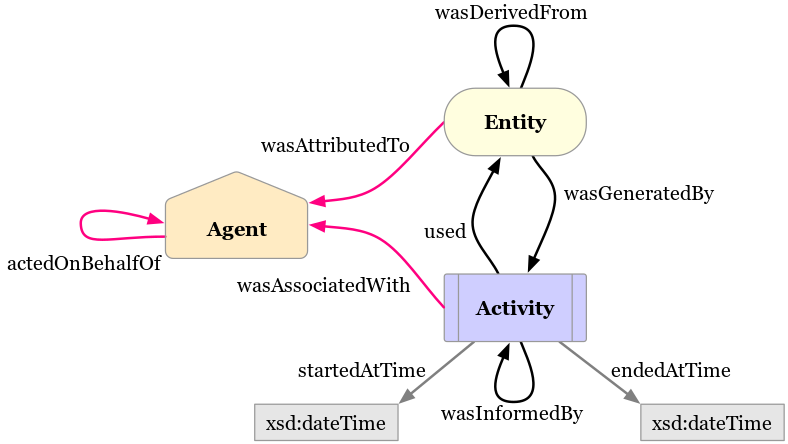
\includegraphics[width=0.8\linewidth]{img/prov-o-model.png}
    \caption{Overview of PROV-O model \cite{lebo_prov-o_2013}}
    \label{fig:prov-o-model}
\end{figure}

PROV-O is a generic and domain independent ontology for representing provenance information.
In order for it to be applied to the domain of GDPR compliance, it needs to incorporate the relevant terminology and enable distinction between different types of activities and entities.
Furthermore, PROV-O as a provenance ontology is intended to represent information about activities that have been executed in the past, and is therefore suitable to represent only the ex-post aspect of GDPR compliance processes.

While PROV-O does provide the concept of \texttt{Plan}\footnote{PROV-O defines a \textit{plan} as a set of actions or steps towards some goal. It clarifies on the lack of concepts relevant to plans as - ``\textit{There exist no prescriptive requirement on the nature of plans, their representation, the actions or steps they consist of, or their intended goals.''}} to represent ex-ante information, it does not provide further concepts or relationships to associate the plan with activities and entities\footnote{PROV-O provides the concept of \texttt{Association} which assigns responsibility to an agent for an activity and indicates that the agent had a role in the activity, which can include a \texttt{Plan} associated using the \texttt{hasPlan} property.}.
In order to adopt PROV-O and use the concept of \texttt{Plan} for representing ex-ante information for GDPR compliance, it needs to be extended with the additional concepts and relationships.

\subsubsection{P-Plan - extending PROV-O Plans as Workflows}
P-Plan \cite{garijo_p-plan_2014} extends the concept of \texttt{Plan} in PROV-O towards representing scientific
workflows which enable creating a template of a `step' and linking it to executions of activities.
A \texttt{p-plan:Plan} is a subclass of \texttt{prov:Plan} and is composed of smaller activities or steps (\texttt{p-plan:Step}) that use and generate (as inputs or outputs) variables (\texttt{p-plan:Variable}).
An overview of the relationship between PROV-O and P-Plan is described in \autoref{fig:p-plan-model}.
P-Plan enables the representation of provenance information associated with both ex-ante and ex-post processes by representing them as scientific workflows. It also enables associating plans with their executions, thereby providing a link between ex-ante and ex-post provenance information.
\begin{figure}[htbp]
    \centering
    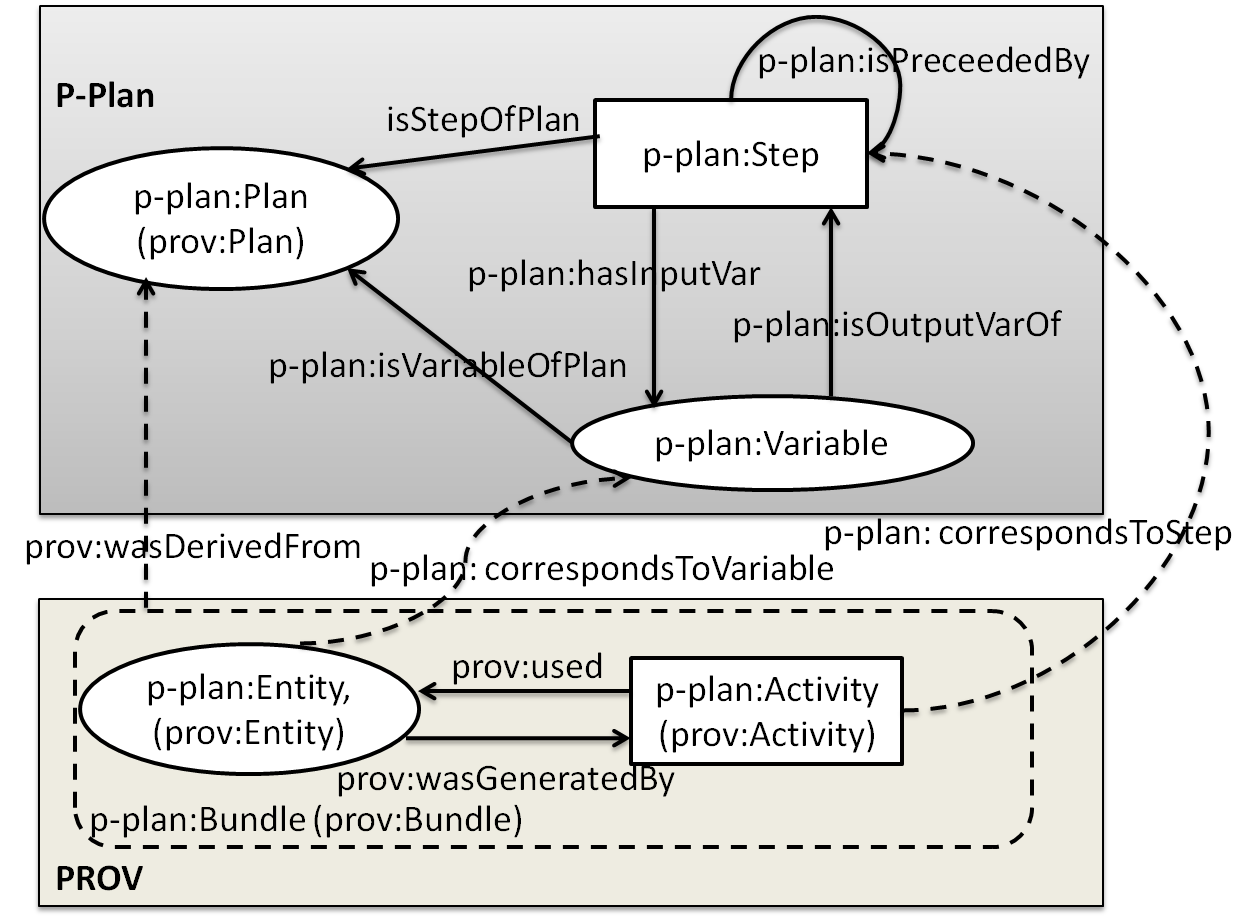
\includegraphics[width=0.75\linewidth]{img/p-plan-model.png}
    \caption{Overview of P-Plan model and its relationship with PROV-O \cite{garijo_p-plan_2014}}
    \label{fig:p-plan-model}
\end{figure}

A \texttt{p-plan:Plan} represents information of `how’ something should happen or a `template’ for executions. A \texttt{p-plan:Activity} is a subclass of \texttt{prov:Activity} and represents the execution of the process described in a \texttt{p-plan:Step}.
A \texttt{p-plan:Entity} is a subclass of \texttt{prov:Entity} that corresponds to a \texttt{p-plan:Variable} in the \texttt{p-plan:Plan}. Therefore, a
\texttt{p-plan:Step} may describe the template including inputs and outputs which can
then be instantiated into multiple instances of \texttt{p-plan:Activity} that can have
distinct inputs to produce different outputs.
As \texttt{p-plan:Plan} extends \texttt{prov:Plan}, which itself extends \texttt{prov:Entity}, it can be
used to treat the \texttt{p-plan:Plan} as an object whose provenance can be tracked using
PROV-O or P-Plan. This makes it possible to express provenance of processes that themselves also describe provenance, thereby creating a history of how plans were formulated and executed over time.

\subsubsection{Extending ontologies for GDPR}
The PROV-O and P-Plan ontologies were extended to represent concepts and relationships of ex-ante and ex-post activities associated with personal data and consent based on requirements of GDPR compliance.
The decision to extend PROV-O and P-Plan with GDPR concepts was made as both ontologies contain generic concepts associated with activities and workflows which can be used for representing information about GDPR compliance, but doing so would be not be intuitive due to the difference in terminology and structuring of information as expected for GDPR compliance.

Extending existing ontologies of PROV-O and P-Plan enables expressing a `template'
or `plan' using \texttt{p-plan:Plan} describing ex-ante activities (as \texttt{p-plan:Step}) that can take place. This template can then be used to denote execution of activities in ex-post phase using \texttt{p-plan:Activity}.
This provides a machine-readable and documented data model of both ex-ante and ex-post activities, whose provenance itself can be expressed (using PROV-O and P-Plan) to record how they were created and how they  change over time.
This is beneficial in documenting the state of a system at a given time as a set of activities that deal with consent and personal data, and
can be helpful in determining changes when the interactions between personal data and an activity change over time.

The extended ontology derived from PROV-O and P-Plan incorporates concepts and relationships associated with GDPR in order to normalise the terminology for representing information associated with GDPR compliance.
The concepts and relationships are derived from the competency questions and linked with their relevant clauses within the GDPR through the use of GDPRtEXT concepts by using \texttt{rdfs:isDefinedBy} and \texttt{rdfs:seeAlso}.
This provides a form of documentation regarding the origin of concepts and their use in the representation of information associated with those clauses of the GDPR.
It also provides a machine-readable link from the ontology to GDPR, which can be used to compare, analyse, and align relevant ontologies.

The extension consists of sub-classing existing concepts in PROV-O and P-Plan to represent specific activities associated with GDPR compliance. 
The use of subclass mechanism preserves the existing concepts and relationships of PROV-O and P-Plan so as to provide compatibility and reuse. This is particularly important in the case of PROV-O as it is the W3C standard for representing provenance information and therefore is more likely to used and expected within the community.
The compatibility also enables packaging the information defined using the ontology as an artefact and defining its provenance as well as planning to provide meta-documentation about how compliance is to be planned and maintained. This is particularly useful to maintain periodic snapshots of organisational processes associated with compliance, and provides the opportunity to automate the querying and validation of information checks within a use-case - as demonstrated in \autoref{chapter:testing}.

\subsection{Ontology Description \& Application}
The resulting ontology is named GDPRov (GDPR Provenance Ontology) and is published online along with its documentation at \url{https://w3id.org/GDPRov/} under the open and permissive CC-by-4.0 license.
The ontology was created, documented, and published using the methodology presented in \autoref{sec:voc:methodology}.
The aim of GDPRov is to provide representations of ex-ante and ex-post activities regarding personal data and consent for GDPR compliance.
It uses the GDPRtEXT ontology to define concepts based on their origin and relevance to clauses within the text of GDPR.

\subsubsection{Overview of GDPRov concepts}
GDPRov extends concepts from PROV-O and P-Plan to represent activities associated with GDPR compliance, with a visual overview provided in \autoref{fig:vocabs:gdprov-overview}.
To that end, it extends the concept of \texttt{p-plan:Plan} in the form of \texttt{Process} to represent ex-ante plans of activities that will take place. The terminology is based on the use of term in commonly used expressions such as `business processes' and `compliance processes'.
Each \texttt{Process} can contain steps (represented by \texttt{p-plan:Step}) to represent activities that interact with data and agents.
To associate steps with a process, the property \texttt{p-plan:isStepOfPlan} is extended as \texttt{isPartOfProcess}.
Another additional property - \texttt{refersToProcess} is also used to enable referring to a process without being a part of it.
Similarly, to associate data (defined in P-Plan as \texttt{p-plan:Variable}) the properties \texttt{p-plan:hasInputVar} and \texttt{p-plan:isOutputVarOf} are extended for activities using inputs and producing outputs respectively.
The ex-post activities in P-Plan are represented by \texttt{p-plan:Activity}.
Data interactions with these activities is represented by \texttt{p-plan:Entity} and the properties \texttt{prov:used} and \texttt{prov:wasGeneratedBy} are used to indicate inputs and outputs respectively.
GDPRov defines steps to indicate automated execution and user interactions regarding collecting data from the user (input) and providing data (output).
To indicate the legal basis associated with a process or a step, the property \texttt{hasLegalBasis} is provided.
\begin{figure}[htbp]
    \centering
    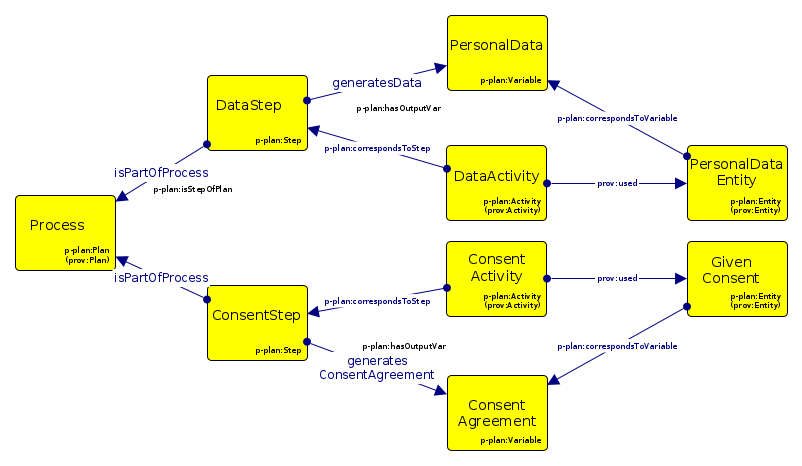
\includegraphics[width=\linewidth]{img/GDProv_relation_prov_pplan.png}
    \caption{GDPRov concepts derived by extending PROV-O and P-Plan}
    \label{fig:vocabs:gdprov-overview}
\end{figure}

\subsubsection{Depicting Data Life-cycle}
Activities associated with the life-cycle of personal data constitute of collecting, processing or using it, storing, sharing, deleting, transferring, transforming, anonymise, and rectifying it. GDPR defines several more categories of actions on data in Article 4-2 in its definition of `processing'.
GDPRov provides broad and abstract processes to represent data access, data archival, data erasure, and data rectification given the need to execute these using several more steps.
GDPRov also provides representations of actions in ex-ante phase as \texttt{DataStep} which extends \texttt{p-plan:Step} and in ex-post phase as \texttt{DataActivity} which extends \texttt{p-plan:Activity}.
These are further extended to distinguish between data collection, data deletion, data sharing, data storage, data archival, data transfer, data transformation, data usage, and rectification of data.
A summary of steps describing a data life-cycle using GDPRov is provided in \autoref{fig:vocabs:gdprov-data-lifecycle}.
\begin{figure}[htbp]
    \centering
    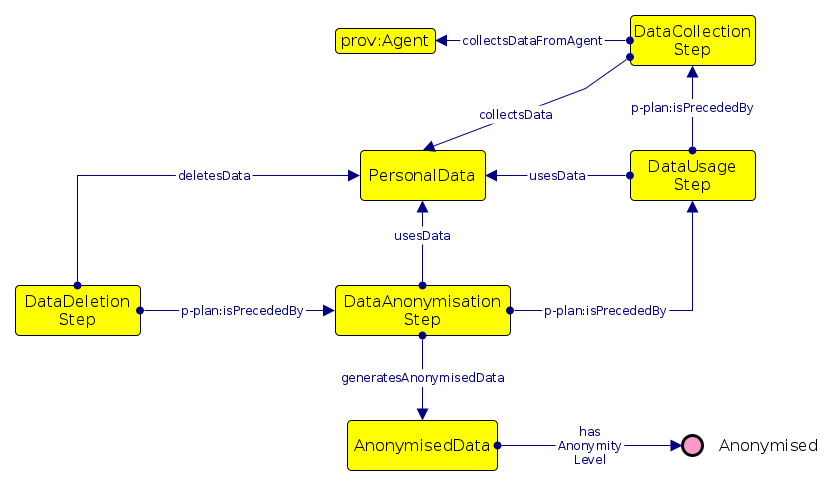
\includegraphics[width=\linewidth]{img/GDPRov_data_lifecycle.png}
    \caption{Example steps depicting data life-cycle using GDPRov}
    \label{fig:vocabs:gdprov-data-lifecycle}
\end{figure}

The anonymisation of data is defined as a sub-class of data transformation to indicate the transformation of data that takes place when anonymising it.
As GDPR obligations are based on the level of anonymity and the capability of de-anonymising it from an organisation's point of view, GDPRov provides the concept of \texttt{anonymisation level} to indicate the state of anonymity the data is in.
GDPRov defines four levels of anonymisation based on existing work in representing anonymous data \cite{hintze_meeting_2017}, which constitute of data that is completely anonymised, completely de-anonymised, pseudo-anonymised, and pseudo-organisational-anonymised where the organisation does not have the data required to de-anonymise it and can thus internally utilise it as if it were completely anonymous data.
The sharing of data consists of interactions with actors or agents, which are represented by \texttt{prov:Agent} and associated with the respective steps and activities using extended properties.

The personal data used within activities is represented by \texttt{PersonalData} which is sub-classed from \texttt{p-plan:Variable} for ex-ante representation and by \texttt{PersonalDataEntity} which is sub-classed from \texttt{prov:Entity} for ex-post representation.
Further categorisation of personal data into anonymised, sensitive, and representing user identifier is provided through sub-classes.

\subsubsection{Depicting Consent Life-cycle}
Activities associated with consent and its life-cycle are represented in ex-ante phase by sub-classing \texttt{p-plan:Step} as \texttt{ConsentStep} and in ex-post phase by sub-classing \texttt{p-plan:Activity} as \texttt{ConsentActivity}.
These are further sub-classed to represent the acquisition, archival, modification, and withdrawal of consent.
Amongst these, withdrawal of consent is defined as sub-class of modification since it modifies the state of consent.
A visual summary of the steps in a consent life-cycle is provided in \autoref{fig:vocabs:gdprov-consent-lifecycle}.
\begin{figure}[htbp]
    \centering
    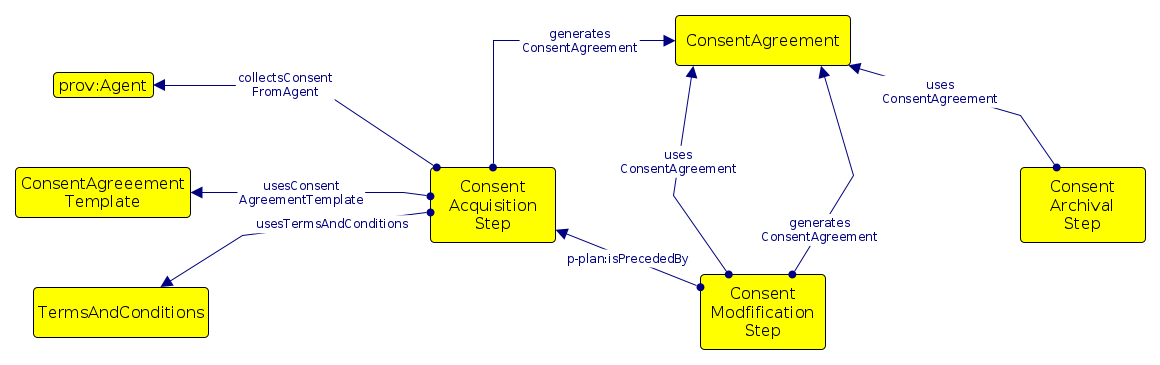
\includegraphics[width=\linewidth]{img/GDPRov_consent_lifecycle.png}
    \caption{Figure describing consent life-cycle defined using GDPRov}
    \label{fig:vocabs:gdprov-consent-lifecycle}
\end{figure}

The artefacts associated with consent and used in activities include the choices or offer of consent provided to the individual and the subsequent consent given by the individual.
To represent these in ex-ante phase, GDPRov provides the concepts of \texttt{ConsentAgreementTemplate} to represent the template offered to collect consent, \texttt{ConsentAgreement} to indicate the given consent, and \texttt{TermsAndConditions} to indicate the policies or terms and conditions.
The corresponding concepts in ex-post phase are \texttt{GivenConsentTemplate}, \texttt{GivenConsent}, and \texttt{TermsAndConditionsEntity}.

\subsubsection{Depicting Compliance-related processes}
In addition to representing activities associated with personal data and consent, GDPRov also provides representations for compliance-related processes.
These include actions such as appointing processor (by a controller), carrying out an impact assessment, marketing and its special case of direct marketing, and monitoring compliance.
Processes are also provided for handling data breaches, which include notifying the controller (by a processor), notifying the data subject, and notifying the data protection authority.
The handling of right provided by the GDPR is represented through sub-classes of \texttt{Process} for data portability, erasure, access personal data, basic info about processing, no automated processing, object to direct marketing, object processing, rectification, restrict processing, transparency, SAR (subject access request).

% \subsubsection{Actors and Agents}
% Controller Representative
% Data Subject
% DPO
% Processor Representative
% Third Party
%     Controller
%         Joint Controller
%     Processor
%         SubProcessor

% \subsubsection{Documentation \& Dissemination}

\subsubsection{Example Use-Case: Querying anonymised sharing of data}
The applicability and usefulness of GDPRov is demonstrated through its use for querying and validation of information for GDPR compliance in \autoref{chapter:testing}.
A simplified example demonstrating such an application through the use of a SPARQL query was published along with the ontology in the peer-reviewed publication \cite{pandit_modelling_2017}, and which is presented in \autoref{code:gdprov:sparql} to demonstrate how GDPRov can assist in the answering of compliance questions for GDPR.
The query uses GDPRov concepts to retrieve data being shared, the specific steps that share it, the anonymisation level of shared data, and the anonymisation steps used to anonymise it. The query is meant to retrieve information relevant in the investigation of data being shared and its anonymity.
\begin{listing}[htbp]
\begin{minted}{sparql}
PREFIX gdprov: <https://w3id.org/GDPRov#>
SELECT ?data ?sharestep ?isAnonymised ?anonymisationStep
WHERE {
    ?data a gdprov:Data .
    ?sharestep a gdprov:DataSharingStep .
    ?sharestep gdprov:sharesData ?data. 
    BIND (
        EXISTS { ?data a gdprov:AnonymisedData . }
        as ?isAnonymised ) .
    OPTIONAL {
        ?anonymisationStep
        gdprov:generatesAnonymisedData ?data .
    }
}
\end{minted}
\caption{SPARQL query representing compliance question \texttt{G5} concerning legal basis for processing}
\label{code:gdprov:sparql}
\end{listing}

\subsubsection{Example Use-Case: Detecting changes in activities for updates to consent}
An example of a use-case is when a data controller updates a plan of processing activities such as when a purpose changes or a new processing operation is added to an existing purpose - and where the legal basis for such processing is consent.
In such cases, the data controller is required to evaluate whether updating an individual's consent is required as per the GDPR based on the changes between the given consent and the new purposes or processing activities. By storing the plans of processing operations using GDPRov, it is possible to compare the old and new versions of a plan, detect changes, and identify whether corresponding updates to consent are needed. 

An exploration of the above change detection was published in the Managing the Evolution and and Preservation of the Data Web workshop co-located with ESWC 2018 \cite{pandit_gdpr-driven_2018} where a model of activities were represented using P-Plan and then compared to identify changes. The use of P-Plan can be substituted with GDPRov when representing GDPR-specific activities.
The publication explored the change when an existing plan is updated to remove the step of sending advertisements. 

The change detection, visualised in \autoref{fig:vocabs:gdprov-change-detection}, is based on identifying the differences between the two plans in terms of steps and variables and whether they have been added, removed, or modified.
In the figure, the change reflects the removal of a step - which by itself does not require any changes to a given consent since no new purposes have been added to an existing given consent.
Using this approach, the detected change can be analysed - manually for complex and legal interpretations while automatically for simpler or simplified graphs - and used to identify whether corresponding changes are necessary based on compliance obligations.
\begin{figure}[htbp]
    \centering
    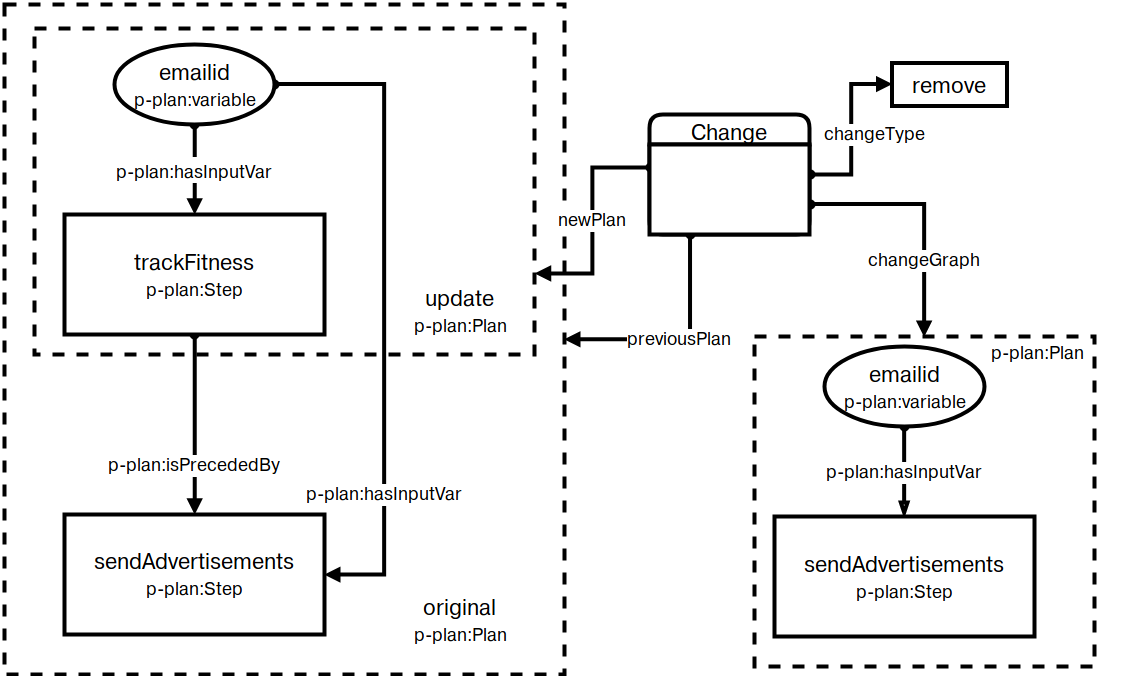
\includegraphics[width=\textwidth]{img/GDPRov-change-detection.png}
    \caption{Modelling changes in workflows using P-Plan \cite{pandit_gdpr-driven_2018}}
    \label{fig:vocabs:gdprov-change-detection}
\end{figure}

\subsection{Evaluation}\label{sec:voc:gdprov:evaluation}
The ontology assessment was based on the methodology outlined in \autoref{sec:voc:methodology} regarding the criterion for evaluation of the quality of ontology and its documentation.
The ontology was used in two applications developed to demonstrate use of SPARQL to query information (see \autoref{sec:testing:sparql}) and SHACL to validate information for GDPR compliance (see \autoref{sec:testing:shacl}). The experience was used to identify suitability of GDPRov in representing the required information, and led to addition of \texttt{ConsentAgreementTemplateBundle} as a concept for convenience in representing `bundled' consent requests and provisions based on consent workflows on a website where a single dialogue is used to collect consent involving multiple distinct purposes and third parties.

GDPRov was published \cite{pandit_modelling_2017} as a peer-reviewed publication in the Workshop on Society, Privacy and the Semantic Web - Policy and Technology (PrivOn) co-located with the 16th International Semantic Web Conference (ISWC). The workshop provided reviews from domain experts in the privacy, legal, and semantic web domains; with ISWC being a top-tier conference in the semantic web domain.

To date, the publication has received 18 citations to date (excluding self-citations) on Google Scholar\footnote{\url{https://scholar.google.com/scholar?cites=2287149512924017207}} of which 2 are deliverables of the CitySPIN research project (see \autoref{sec:sota:gdpr-semweb}).
% Of these, the publications associated with PrOnto \cite{palmirani_pronto_2018,palmirani_pronto_2018-1} incorrectly conclude that ``GDPRov aims to describe the provenance of the consent and data lifecycle in the light of the Linked Open Data principles such as Fairness and Trust'' - since the basis of GDPRov is the scientific workflow model similar to the one used within PrOnto.
% The publication of a PROV-O model representing activities for GDPR compliance by Ujcich et al. \cite{belhajjame_provenance_2018} cites GDPRov as a relevant approach with the comparison to GDPRov specified as - ``Our model allows for more flexible specifications of how data can be used (i.e.,under consent for particular purposes while being legally valid for a period of time). Furthermore, our model focuses on temporal reasoning and online data usage control, whereas it is not clear how amenable GDPRov is to such reasoning or enforcement.'' While the example provided in the publication does provide temporal annotation of activities for GDPR compliance - these are achieved through the use of PROV-O rather than specialised classes using GDPR terminology. Since GDPRov extends PROV-O, it supports such use of inherent PROV-O concepts. In addition, GDPRov provides expression of ex-ante activities and workflows which cannot be expressed using the model proposed by Ujcich et. al.
A publication describing an approach for annotating DFDs (data flow diagrams) with information for analysing compliance \cite{debruyneOntologyRepresentingAnnotating2019}  utilises GDPRov to represent personal data as an entity used in activities. The publication provides an ontology for representation of DFDs to abstract the processing operations as data flows based on the argument of their ease of analysis as compared to workflows.

\subsubsection{Fulfilment of Competency Questions}
An assessment of the extent to which GDPRov satisfies the competency questions by providing concepts and relationships is presented as part of its evaluation.
The competency questions, summarised in \autoref{sec:gdprov:cq}, were used to guide the development of the ontology and therefore used to evaluate if the ontology meets the requirements of representing this information.
\autoref{table:gdprov:cq} lists the concepts and properties relevant to answer the competency question (with \textit{N/S} used to indicate not in scope).
\begin{table}[htbp]
\footnotesize
\centering
\rowcolors{1}{}{gray!10}
\begin{tabularx}{\linewidth}{|l|X|p{5cm}|l|}
\caption{Concepts in GDPRov for answering competency questions} \\ \hline
\label{table:gdprov:cq}
\textbf{CQ} & \textbf{Class} & \textbf{Property} & \textbf{Phase} \\ \hline
\multicolumn{4}{|l|}{\textbf{Actors and Agents involved in activities}}  \\ \hline
\textit{CMQ2} & \textit{Controller}, \textit{ControllerRepresentative}, \textit{DPO} &  &  \\ \hline
\textit{CMQ17} & \textit{Processor}, \textit{ProcessorRepresentative}, \textit{DPO} &  &  \\ \hline
\textit{CMQ35} & \textit{DataSubject} &  &  \\ \hline
\multicolumn{4}{|l|}{\textbf{Details of processing}}  \\ \hline
\textit{CMQ3} & \textit{Process} & \textit{refersToProcess} & \textit{Ex}-\textit{ante} \\ \hline
\textit{CMQ4} & \textit{DataSubject} &  &  \\ \hline
\textit{CMQ5} & \textit{PersonalData}, \textit{SensitiveData} & \textit{usesData} & \textit{Ex}-\textit{ante} \\ \hline
 & \textit{PersonalDataEntity}, \textit{SensitiveDataEntity} &  & \textit{Ex}-\textit{post} \\ \hline
\textit{CMQ6} & \textit{DataSharingStep} & \textit{sharesData}, \textit{sharesDataWith} & \textit{Ex}-\textit{ante} \\ \hline
 & \textit{DataSharingActivity} & \textit{hasSharedDataWith} & \textit{Ex}-\textit{post} \\ \hline
\textit{CMQ7} & \textit{ThirdParty} & \textit{sharesDataWithThirdParty} & \textit{Ex}-\textit{ante} \\ \hline
\textit{CMQ8} & \textit{ThirdParty} & \textit{sharesData}, \textit{sharesDataWith} & \textit{Ex}-\textit{ante} \\ \hline
\textit{CMQ9} & \textit{N}/\textit{S} & \textit{N}/\textit{S} &  \\ \hline
\textit{CMQ10} & \textit{N}/\textit{S} & \textit{N}/\textit{S} &  \\ \hline
\textit{CMQ11} & \textit{DataStorageStep} & \textit{usesData}, \textit{generatesData} & \textit{Ex}-\textit{ante} \\ \hline
 & \textit{DataStorageActivity} &  & \textit{Ex}-\textit{post} \\ \hline
\textit{CMQ12} & \textit{N}/\textit{S} & \textit{N}/\textit{S} &  \\ \hline
\textit{CMQ13} & \textit{N}/\textit{S} & \textit{N}/\textit{S} &  \\ \hline
\textit{CMQ26} &  & \textit{hasLegalBasis} &  \\ \hline
\multicolumn{4}{|l|}{\textbf{Lifecycle of data}} \\ \hline
\textit{CMQ28} & \textit{DataCollectionStep} & \textit{collectsData} & \textit{Ex}-\textit{ante} \\ \hline
 & \textit{DataCollectionActivity} &  & \textit{Ex}-\textit{post} \\ \hline
\textit{CMQ29} & \textit{DataCollectionStep} & \textit{collectsDataFromAgent} & \textit{Ex}-\textit{ante} \\ \hline
 & \textit{DataCollectionActivity} & \textit{collectedDataFromAgent} & \textit{Ex}-\textit{post} \\ \hline
\multicolumn{4}{|l|}{\textbf{Anonymisation}} \\ \hline
\textit{CMQ31} & \textit{DataAnonymisationStep}, \textit{AnonymisedData} &  & \textit{Ex}-\textit{ante} \\ \hline
 & \textit{DataAnonymisationActivity}, \textit{AnonymisedDataEntity} &  & \textit{Ex}-\textit{post} \\ \hline
\textit{CMQ32} & \textit{PersonalData}, \textit{SensitiveData} & \textit{hasAnonymityLevel} & \textit{Ex}-\textit{ante} \\ \hline
\multicolumn{4}{|l|}{\textbf{Activities associated with Consent}} \\ \hline
\textit{CMQ48} & \textit{ConsentStep}, \textit{ConsentAcquisitionStep}, \textit{ConsentModificationStep}, \textit{ConsentArchivalStep}, \textit{ConsentAgreement}, \textit{ConsentAgreementTemplate} & \textit{usesConsentAgreement}, \textit{generatesConsentAgreement} & \textit{Ex}-\textit{ante} \\ \hline
 & \textit{ConsentActivity}, \textit{AcquireConsentActivity}, \textit{ArchiveConsentActivity}, \textit{ModifyConsentActivity}, \textit{GivenConsent}, \textit{GivenConsentTemplate} & \textit{collectedConsentFromAgent} & \textit{Ex}-\textit{post} \\ \hline
\textit{CMQ49} & \textit{ConsentAgreementTemplate} &  & \textit{Ex}-\textit{ante} \\ \hline
 & \textit{GivenConsentTemplate} &  & \textit{Ex}-\textit{post} \\ \hline
\end{tabularx}
\end{table}

% Some questions which were not considered in scope regarding expression of activities are marked with \textit{N/S}. 
Questions not in scope (marked as \textit{N/S} either require clarity from authoritative sources regarding interpretation of information to provide a concrete design pattern or have multiple possible representations of which it cannot be determined which is more useful from a legal compliance point of view. Examples include location of recipients - which can be expressed either through an property/annotation associated with a data sharing activity or attached with a particular third party; and specifying time limits or duration or conditional events associated with data storage and deletion periods. These have been identified as future work regarding further development of the ontology based on differing interpretations of representation, complexity of specifying values such as ``EU membership'' and  ``as long as required'', and the pending expert opinion of legal authorities on these issues through courts or executive decisions.

The presented evaluation demonstrates GDPRov satisfies the requirements of answering competency questions regarding representation of activities and identifies those that are needed to be resolved as future work based on availability of legal opinion and decisions. GDPRov thus fulfils the research objective $RO3(b)$ by providing representations of activities associated with personal data and consent in ex-ante and ex-post phases.

\subsubsection{Comparison with SotA}
The representation of process flows and activities associated with GDPR compliance in existing approaches was presented and analysed as part of the state of the art in \autoref{sota:analysis:process-flows}.
The attributes for this analysis involved the features or concepts that could be represented using the specified approach and the basis for the representation in existing vocabularies and standards.
The analysis demonstrated the existence of a variety of approaches that utilised the existing standards of PROV-O and BPMN to model GDPR-specific information regarding process flows and activities in both ex-ante and ex-post phase. It was also found that approaches modelling both ex-post and ex-ante phases exist and utilise PROV-O as their basis for representation of information.

A comparison of GDPRov with the SotA is provided in \autoref{table:gdprov:sota} using the same attributes used for analysis.
The table lists the features supported by each approach through the notation of a check mark (\cmark).
The column headings corresponding with expression of information supported by an approach, and use the following abbreviations - (Repr): method used for representation of process flow; (EA): whether it permits Ex-ante modelling; (EP): whether it permits Ex-post modelling; (Pu): whether Purpose can be specified; (Pr): whether Processing can be specified; (DS): if Data Sharing can be modelled; (Rp): if Recipients are associated with data sharing; (St): whether Data Storage occurs; (Rg): if provision of Rights can be modelled; and (LB): if Legal Basis can be associated with a process flow.
% Table GDPRov vs SotA
\begin{table}[htbp]
\footnotesize
\centering
\rowcolors{1}{}{gray!10}
\begin{tabularx}{\textwidth}{|l|l|X|X|X|X|X|X|X|X|X|}

\caption{Comparison of GDPRov with SotA}\label{table:gdprov:sota} \\ \hline
\textbf{Work} & \textbf{Repr} & \textbf{EA} & \textbf{EP} & \textbf{Pu} & \textbf{Pr} & \textbf{DS} & \textbf{Rp} & \textbf{St} & \textbf{Rg} & \textbf{LB} \\ \hline
\rowcolor[gray]{0.8}
\textbf{GDPRov} & PROV-O,P-Plan & \cmark & \cmark & \cmark & \cmark & \cmark & \cmark & \cmark & \cmark & \cmark  \\ \hline
SPECIAL & PROV-O & \cmark & \cmark & \cmark & \cmark & \cmark & \cmark & \cmark &  &  \\ \hline
SPL+CitySPIN & PROV-O & \cmark & \cmark & \cmark & \cmark & \cmark & \cmark & \cmark &  &  \\ \hline
MIREL & PWO & \cmark &  & \cmark & \cmark &  &  & \cmark & \cmark &  \\ \hline
MRL+DAPRECO & PWO & \cmark &  & \cmark & \cmark &  &  & \cmark & \cmark &  \\ \hline
BPR4GDPR &  & \cmark & \cmark & \cmark & \cmark & \cmark & \cmark &  &  &  \\ \hline
Ujcich et al. & PROV-O &  & \cmark & \cmark & \cmark & \cmark & \cmark & \cmark & \cmark & \cmark \\ \hline
Lodge et al &  & \cmark &  & \cmark &  &  &  &  &  &  \\ \hline
Tom et al & BPMN & \cmark &  &  & \cmark & \cmark & \cmark & \cmark & \cmark &  \\ \hline
LUCE &  & \cmark & \cmark &  &  & \cmark & \cmark &  &  &  \\ \hline
Sion et al &  & \cmark &  & \cmark & \cmark & \cmark & \cmark & \cmark &  & \cmark \\ \hline
privacyTracker &  & \cmark & \cmark &  &  & \cmark & \cmark &  &  &  \\ \hline
Basin et al &  & \cmark &  & \cmark &  &  &  &  &  &  \\ \hline
RestAssured &  &  &  & \cmark & \cmark & \cmark & \cmark & \cmark &  &  \\ \hline
\end{tabularx}
\end{table}

The table demonstrates that GDPRov supports all of the features, and is the only one currently providing all of them. However, this analysis only takes into consideration the abstract existence or provision of features and does not take into consideration the context of the approach or its granularity. For example, while an approach may provide representation of data storage concepts, there are additional features such as storage duration, condition, form or medium, security, and policy which are also relevant to the evaluation of GDPR compliance.
These are highly dependant on individual use-cases and domains, and contain existing work which can be used to represent them such as the Time ontology \cite{cox_time_2017} for temporal annotations and the ODRL ontology \cite{iannella_odrl_2018} for policies.
Since the scope of GDPRov is limited to the expression of information regarding activities in ex-ante and ex-post phases, the representation of such granular attributes is not within the scope and is therefore not considered in its evaluation or comparison with the SotA.

Regarding the expression of information as being in either ex-ante or ex-post phase - GDPRov is the only approach to do so using the existing ontologies of PROV-O and P-Plan based on the scientific workflow model which is useful in the investigation of executions based on a plan and the association of information between ex-ante and ex-post phases. The use of PWO \cite{gangemi_publishing_2017} in the MIREL project also follows a similar rationale though it does not provide the same extent of concepts and representations as GDPRov.
In addition, the utilisation of PROV-O as its base ontology enables information represented using GDPRov to be captured and recorded as provenance information using PROV-O or GDPRov itself. This provides capabilities for documentation the evolution of a system as well as representation the state of compliance at a given moment in time.
This feature is shared by all approaches that utilise a provenance based ontology at their core, and especially the ones that utilise PROV-O as it is a well-recognised and adopted standard.
The combination of PROV-O and P-Plan enables a flexible representation of activities by specifying their constituent steps and involved artefacts at an arbitrary level of granularity while providing annotations and classes to link these with the GDPR. In this, GDPRov is unique and novel within the SotA.

Based on this, GDPRov's novelty within the SotA is based on it being one of the few approaches using PROV-O to represent activities for GDPR compliance in both ex-ante and ex-post phases. GDPRov is also novel in its provision of concepts associated with GDPR and the arbitrary granularity afforded by the use of PROV-O and P-Plan to link information in ex-ante and ex-post phases.
Furthermore, GDPRov is one of the few approaches to be available under an open and permissive license (CC-by-4.0) thereby enabling its use, adoption, and further evolution.

\subsubsection{Application to external use-case from SPECIAL project}\label{sec:gdprov:use-case:SPECIAL}
% description of the use-case
The SPECIAL project uses a scenario\footnote{NOTE: the scenario explicitly mentions use of an immutable distributed ledger developed by the SPECIAL project to provide transparency and log accountability regarding metadata. This is omitted from the adapted use-case used to evaluate GDPRov.} to motivate their work and demonstrate the use of developed technologies in their deliverables (D1.7 \cite{bonatti_d1.7_2018}) and peer-reviewed publications (\cite{kirrane_scalable_2018}).
In this section, the scenario is adapted as an external use-case to evaluate GDPRov's suitability to express the required concepts.

The use-case is summarised as follows with GDPR concepts added in parenthesis for relevance: Sue (Data Subject) buys a wearable appliance for fitness tracking from BeFit (Data Controller), and is presented with an informed consent request that describes collection of biomedical parameters such as heart rate (Personal Data), and how they will be processed, stored in BeFit's cloud and transmitted for the purposes of: giving Sue feedback on her activity, such as calories consumption; and creating an activity profile that will be shared with other companies for targeted ads related to fitness - an optional purpose which Sue opts-in. After two years, Sue starts receiving annoying SMS messages from a local gym that advertise its activities. Sue discovers the following facts: (i) the gym has an activity profile referring to Sue, that, due to the appliance’s malfunctioning, reports that she is not doing any physical exercise; (ii) the gym received the profile from BeFit, associated with a policy that allows the gym to send targeted ads to Sue based on the profile; (iii) BeFit built the profile by mining the data collected by the appliance; and (iv) all these operations are permitted by the consent agreement previously signed by Sue and BeFit. Using this information BeFit and the gym prove that they used Sue’s data according to the given consent. Sue now asks both BeFit and the gym to delete all of her data. 

The use-case is accompanied with information on its interpretation in terms of GDPR terminology \cite{bonatti_d1.7_2018} and its representation using the SPECIAL vocabularies \cite{kirrane_scalable_2018}. To represent the use-case using GDPRov, the concepts used by SPECIAL are mapped or aligned to their closest relative concepts within GDPRov (see \autoref{table:gdprov:use-case:SPECIAL}) with its RDF/Turtle representation provided in \autoref{code:gdprov:use-case:special}. The SPARQL queries used to retrieve information depicted by statements (i) to (iv) in the scenario are provided in \autoref{code:gdprov:use-case:special-sparql}. The RDF representation and SPARQL query utilised a simplified representation of the scenario to present only the facts essential to the answering of questions. 
\begin{center}
\footnotesize
\begin{tabularx}{\textwidth}{|p{0.35\linewidth}|X|X|}
\caption{GDPRov concepts to represent external use-case from SPECIAL} \label{table:gdprov:use-case:SPECIAL} \\
\toprule
\textbf{Statement} & \textbf{GDPRov concept} & \textbf{SPECIAL concept} \\
\midrule
\endhead
Sue & \texttt{DataSubject} & \texttt{DataSubject} \\ \hline
BeFit & \texttt{DataController} & \texttt{Controller} \\ \hline
Biomedical parameters, heart rate, calories consumption, activity profile & \texttt{PersonalData} & \texttt{Data} \\ \hline
Collect data & \texttt{DataCollectionActivity} & \texttt{Collect} \\ \hline
Provide feedback on activity & \texttt{Purpose} & \texttt{Purpose} \\ \hline
Give consent (opt-in) & \texttt{AcquireConsentActivity} & \texttt{ConsentAssertion} \\ \hline
Targeted ads related to fitness & \texttt{Purpose} & \texttt{Purpose} \\ \hline
Share data & \texttt{DataSharingActivity} & \texttt{Recipient} \\ \hline
Gym & \texttt{ThirdParty} & \texttt{Recipient} \\ \hline
Consent agreement & \texttt{GivenConsent} & \texttt{LogEntryContent} \\ \hline
Delete data & \texttt{DataDeletionActivity} & N/A \\ \hline
Withdraw consent & \texttt{WithdrawConsentActivity} & \texttt{ConsentRevocation} \\
\bottomrule
\end{tabularx}
\end{center}
\begin{listing}[htbp]
\begin{minted}{turtle}
# Entities
:Sue a gdprov:DataSubject .
:BeFit a gdprov:DataController .
:Gym a gdprov:ThirdParty .
# Personal Data
:Biomedical_Parameters a gdprov:PersonalData .
:Activity_Profile a gdprov:PersonalData .

# Register with BeFit, given consent, and generate activity profile
:Registration a gdprov:Process .
:Sue_consent a gdprov:GivenConsent, gdprtext:LawfulBasisForProcessing .
:Collect_consent a gdprov:AcquireConsentActivity ;
    gdprov:isPartOfProcess :Registration .
    gdprov:collectedConsentFromAgent :Sue ;
    gdprov:generatedConsent :Sue_consent .
:Collect_data a gdprov:DataCollectionActivity ;
    gdprov:isPartOfProcess :Registration ;
    prov-o:wasInformedBy :Collect_consent ;
    gdprov:collectedDataFromAgent :Sue ;  # from Sue's device
    gdprov:generatedData :Activity_Profile .

# Share activity profile with Gym
:Targeted_ads_related_to_fitness a gdprov:Process ;
    gdprov:hasLegalBasis :Sue_consent .
:Share_data a gdprov:DataSharingActivity ;
    :sharedData :Activity_Profile ;
    :hasSharedDataWith :Gym .
# Gym receives Sue's activity profile from BeFit
:Collect_data_from_BeFit a :DataCollectionActivity ;
    gdprov:collectedDataFromAgent :BeFit ;
    gdprov:involvesAgent :Sue ;
    gdprov:refersToProcess :Targeted_ads_related_to_fitness ;
    gdprov:generatedData :Activity_Profile . # Gym copy of data

# Sue withdraws consent
:Withdraw_consent a gdprov:WithdrawConsentActivity ;
    prov:invalidated :Sue_consent .
# BeFit and Gym deleted the activity profile
:Delete_data a gdprov:DataDeletionActivity ;
    prov:invalidated :Activity_Profile ;
    prov:wasInformedBy :Withdraw_consent .
\end{minted}
\caption{GDPRov representation of external use-case from SPECIAL}
\label{code:gdprov:use-case:special}
\end{listing}
\begin{listing}[htbp]
\begin{minted}{sparql}
# Query (i)
# retrieves :Activity_Profile as personal data shared with Gym
# queried over Gym's records
SELECT ?personal_data 
WHERE {
    ?personal_data a gdprov:PersonalData .
    ?activity gdprov:generatedData .
    ?activity (gdprov:collectedDataFromAgent|gdprov:involvesAgent) :Sue .
}

# Query (ii)
# retrieves :BeFit as data source
# retrieves :Targeted_ads_related_to_fitness as purpose
# queried over Gym's records
SELECT ?party, ?purpose 
WHERE {
    ?activity gdprov:generatedData :Activity_Profile .
    ?activity gdprov:collectedDataFrom ?party .
    ?activity gdprov:refersToProcess ?purpose .
}

# Query (iii)
# retrieves :Sue as data source (as Sue's device)
# queried over BeFit's records
SELECT ?data_source 
WHERE {
    ?activity_profile gdprov:generatedData :Activity_Profile .
    ?activity_profile gdprov:collectedDataFromAgent ?data_source .   
}

# Query (iv)
# retrieves :Sue_consent as the legal basis for data collection and mining
# queried over BeFit's records
SELECT ?legal_basis 
WHERE {
    {
        ?activity gdprov:generatedData :Activity_Profile .
    } UNION {
        ?activity gdprov:sharedData :Activity_Profile .
        ?activity gdprov:hasSharedDataWith :Gym .
    }
    ?activity (
            gdprov:hasLegalBasis|
            (gdprov:isPartOfProcess/gdprov:hasLegalBasis))
        ?legal_basis .
}


\end{minted}
\caption{SPARQL queries using GDPRov for external use-case from SPECIAL}
\label{code:gdprov:use-case:special-sparql}
\end{listing}

Through the representation of the concepts within the scenario and the use of SPARQL, GDPRov is shown to support the representation and answering of questions within the scenario. While the scenario relies on the use of SPECIAL's policy-based vocabulary and the immutable distributed ledger to store and retrieve information regarding given consent and the processing activities carried out by BeFit and the Gym, these have not been replicated the above representation as storage mechanisms are not within scope for this work.

One important conclusion from the above exercise is the representation of given consent, where SPECIAL vocabularies represent the given consent as a policy using OWL2 \cite{kirrane_scalable_2018}.
In comparison, GDPRov does not represent information provided in the consent request and given consent, but instead records it as an activity and associates the generated consent as an artefact representing a legal basis with the purposes (specified using \texttt{gdprov:Process}) that rely on it. 
This is the consequence of GDPRov focusing on the representation of activities which does not concern the representation of consent.
A consent-centric representation of this same scenario is presented in \autoref{sec:gconsent:use-case:SPECIAL} which uses GConsent to represent the scenario as interactions between consent states.

% \subsubsection{Application to external use-case from Ujcich et al.}
% Ujcich et al. present a similar (to the above) scenario in their demonstration of a provenance vocabulary based on the GDPR \cite{belhajjame_provenance_2018}. 
% The scenario concerns Alice, a customer, who registers with a retailer and provides name, address, and credit card number; gives consent to store these and use for purchases made, and also consents to use of name and address to receive marketing. 
% At some period of time, the retailer employs a third-party for marketing and provides it with Alice’s name and address based on the given consent.
% After some more period of time, Alice no longer wishes to receive marketing and withdraws her consent.
% The investigation of compliance presented in the publication utilises two questions related to the scenario, which are: (i) Was Alice’s personal data used for marketing purposes after Alice withdrew her consent?; and (ii) Was Alice’s personal data used for marketing purposes after Alice withdrew her consent?

% Ujcich et al. represent the scenario as a series of activities using PROV-O

% % breakdown into requirements
% % select concepts from GDPRov to represent requirements - ex-ante and ex-post
% % representation Turtle code
% % analysis - what is possible and what isn't
% % comment on deficiencies or advantages of GDPRov

% \subsubsection{Application to External Use-case: Ujcich et al.}
% % description of the use-case
% % breakdown into requirements
% % select concepts from GDPRov to represent requirements - ex-ante and ex-post
% % representation Turtle code
% % analysis - what is possible and what isn't
% % comment on deficiencies or advantages of GDPRov

\subsection*{Summary}
GDPRov is part of the second major contribution of this thesis. It provides an ontological representation of ex-ante and ex-post activities associated with personal data and consent for GDPR compliance.
It thus fulfils the research objective $RO3(b)$ as outlined in \autoref{sec:intro:RQ}. 
The use of GDPRov makes it possible to indicate the plans associated with how personal data and consent is collected, used, stored, shared, and erased.
It also enables the representation of logs for activities that act over personal data and consent.

At the time of this undertaking (in 2016-2017), no other vocabulary was found that represented information about activities associated with GDPR compliance.
The work presented as state of the art in \autoref{chapter:sota} and demonstrating existence of approaches for representing information about GDPR processes were published after the publication of GDPRov. Of these approaches, some also utilise PROV-O to represent provenance of activities as seen through the analysis presented in \autoref{sota:analysis:process-flows}. The differentiating factor of GDPRov is the use of PROV-O and P-Plan as distinct ontologies representing ex-ante and ex-post phases of activities based on the scientific workflow model - which is novel within the state of the art. Another differentiating factor is the use of GDPRtEXT to define concepts and relationships within GDPRov, thereby linking the use of ontology with the legal concepts it was derived from.

Approaches within the state of the art, for example SPECIAL (\autoref{sec:sota:SPECIAL}), demonstrate the applicability of provenance vocabularies in maintaining, querying, and assessing provenance logs represented using PROV-O for GDPR compliance.
While SPECIAL also provides ex-ante compliance assessment by using the same data model and logging it as a request instead of execution \cite{dullaert_d3.4_2019}, GDPRov further expands on the use of provenance to include the representation of plans or templates to indicate the association between activities in ex-ante and ex-post phases of compliance.
% GConsent
\section{GConsent - Ontology of Consent Information for GDPR Compliance}\label{sec:voc:GConsent}
GConsent is a semantic web ontology for representing contextual information about consent based on requirements of GDPR compliance. 
GConsent aims to model the context, state, and provenance of consent as an entity.
Its scope is limited to consent as defined in the GDPR and is intended towards assisting in the modelling of information associated with compliance.
It uses GDPRtEXT to denote the origin and relevance of its concepts within the text of the GDPR.

GConsent is the outcome of applying the methodology presented in \autoref{sec:voc:methodology} to identify and represent information about consent and its life-cycle as required to determine compliance.
For this, the information presented in \autoref{chapter:background} was used to identify the validity of consent defined by GDPR with the requirements and compliance questions presented in \autoref{chapter:information} used as competency questions.
GConsent is published online\footnote{\url{https://w3id.org/GConsent}} with its documentation under the open and permissive license of CC-by-4.0 and its code repository\footnote{\url{https://github.com/coolharsh55/GConsent/}}.

The design of GConsent was influenced by a real-world use-case for managing the consent information based on GDPR compliance requirements, as mentioned earlier in \autoref{sec:info:compliance-questions-methodology}.
In particular, the design of the ontology underwent several iterations based on whether the ontology should model an association or dependency between purposes and processing operations associated with consent. The final iteration, presented here, provides a separation between purpose and processing operations - which is similar to the other representations of consent within the SotA.

\subsection{Distinction with existing work in state of the art}
Information about consent needs to be maintained and shared by multiple parties which includes the data subject who gives consent, controller who uses it as a legal basis, processor who might be collecting from, and authorities who would evaluate its validity. This requires the information about consent across its life-cycle to be maintained in an representation that is interoperable as outlined in the model in \autoref{sec:info:model}.

From the existing work analysed in state of the art in \autoref{chapter:sota}, the focus of approaches for consent is mostly on the concept of `given' consent i.e. consent provided by the data subject and used as a legal basis by the controller. There is a lack of work regarding representing other `states' of consent within its life-cycle as an entity or representation of agreement which are relevant to its use as a legal basis in the determination of processing of personal data and its compliance under GDPR.
Examples of such states are `not given', `refused', `withdrawn' which cannot be modelled in the same manner as `given consent' as they do not reflect the same information as given consent but are still relevant when associated with a particular instance of processing the data subject's personal data. The state of a consent reflects its status for use as legal basis and is also relevant in the management of information from an organisation's perspective.

Apart from the notion of states, the existing approaches also lack modelling representations for events such as delegation, and associations with third parties regarding consent which have an effect on its validity regarding compliance.
GConsent aims to fill this gap, and therefore to provide novelty and contribution by representing a more cohesive and complete representation of information associated with consent under the GDPR.

\subsection{Relationship with GDPRov}
GConsent builds upon and is complimentary to the representation of consent in GDPRov.
The definition of consent as an entity involved in activities is sufficient to express its life-cycle and provenance by using GDPRov. This includes the ex-ante representation of information provided to collect consent and its subsequent agreement by the individual to produce given consent, which is then used within activities as a legal basis, and may be modified, withdrawn, or revoked - signalling its effective end of life-cycle.
While GDPRov is sufficient to represent these states of consent as an entity along with information about activities acting on it, the primary focus of GDPRov is about expressing the information from the point of view of recording its use within activities.
Managing consent as a legal basis involves consideration of information such as purpose of processing, recipients, and contextual information such as medium of provision and collection, and situations such as delegation.

GConsent aims to provide a consent-centric representation of these information categories by providing concepts relevant to the resolution of valid consent as defined by requirements of GDPR compliance. In this, the use of provenance concepts show an overlap with GDPRov.
This is resolved through the differing scopes of the two ontologies, where concepts defined within GDPRov can also be defined using corresponding concepts in GConsent and vice-versa. An example of such cohesive usage is demonstrated through the application of developed ontologies for querying and validation of information in \autoref{chapter:testing}.
By having separation between GDPRov and GConsent, the ontologies are modular and therefore provide an adopter the ability to choose only one of them without involving the other.

\subsection{Requirements Gathering and Establishment of Competency Questions}
The scope of consent as represented within GConsent is limited to the definition of consent as provided by Article 4-11\footnote{In this definition, consent is expressed as the indication of a data subject's wishes regarding processing of their personal data. However, this is a legal definition rather than a semantic one as it essentially defines the set of conditions required to be satisfied by some consent before it is considered valid under GDPR. Additionally, `consent' as a social concept has a pre-defined meaning based on its use in the social context. Therefore, referring to consent in the context of GDPR does not only mean given consent but includes all information and states associated with consent which can then be evaluated to assess whether it fits the definition of consent as a legal basis. Technical approaches can use `consent' to indicate the given consent or the set of all consent states within its life-cycle.} of GDPR. 
Other special cases of consent not included within the scope consist of consent defined by Article 9 regarding use of special categories of personal data, Recital 33 regarding use of personal data for scientific research, and Article 8 along with Recital 38 regarding use of children’s personal data.
These were not included within the scope due to their additional requirements and complexity regarding interpretation and representation using semantic web. Additionally, the current lack of real-world use-cases reflecting how these types of consent would function and the legal guidance on their compliance requirements is noticeably absent in the context of GDPR.

GConsent is primarily based on the notion of consent as a legal basis under Article 6 of the GDPR. The conditions defined in Article 7, Recital 42, and Recital 43 provide the requirements for consent to be considered or determined valid as per the requirements of GDPR.
The Data Controller bears the burden of demonstrating proof and satisfaction of requirements for consent to be considered valid as per Recital 42. This requires demonstrable proof that the data subject provided the consent and that it was valid as per the obligations specified in the GDPR.

For consent to be informed it is necessary to provide information to the data subject which includes the specific purposes of processing the personal data.
GDPR also provides data subjects with the right to modify or withdraw consent as defined in Article 7-3.
When consent is withdrawn the processing carried out done prior to the withdrawal is considered valid under the given consent which was in effect as the legal basis during that period of time.

Through this, a rudimentary summary of information or attributes associated with `consent' as defined by GDPR is expressed as:
\begin{itemize}
    \item Data Subject the consent is about
    \item Personal Data associated with consent
    \item Processing operations or categories the consent is about, with data storage and data sharing having additional information requirements
    \item Purposes the consent is about
    \item Entity/Agent/Actor the consent is provided to
    \item Recipients of data or categories of recipients if any
\end{itemize}
These attributes are sufficient to provide a simplified representation of consent, and are used in existing approaches within the state of the art - such as the model of consent in SPECIAL vocabularies \cite{bonatti_special_2018}. However, these attributes are not sufficient by themselves to determine the validity of consent as they lack information about the context the consent was given in as well as changes to its state.

Therefore, further attributes associated with consent are identified and expressed as:
\begin{itemize}
    \item Entity/Agent/Actor that provided the consent - relevant in the case of delegation
    \item Entity/Agent/Actor that revoked, withdrew, or invalidated the consent - relevant in the case of delegation, and authoritative actions such as by regulators or courts
    \item Status of consent at a given period in time
    \item Contextual information regarding request and giving of consent such as - location, medium, timestamp, expiry
    \item Contextual information regarding revocation, withdrawal, and invalidation of consent such as - location, medium, timestamp, expiry
\end{itemize}
In addition to these, the provenance of how consent was requested and obtained is also important.
Specifically, the information about the specific process and artefacts used in the provision of request for consent - which must satisfy the GDPR qualitative requirements such as the request being clearly stated and being unambiguous.

To derive the required concepts, competency questions were identified from the compliance questions presented in \autoref{sec:info:compliance-questions} pertaining to given consent (\texttt{CMQ35-CMQ69}) and change in consent state (\texttt{CMQ70-CMQ87}).
These refer to information regarding consent (e.g. \texttt{CMQ35-CMQ40}), the consent was created/given/changed/invalidated (e.g. \texttt{CMQ41-CMQ52}), the context of how consent was created/given/invalidated (e.g. \texttt{CMQ53-CMQ56}), and third parties associated with the consent (e.g. \texttt{CMQ57-CMQ58}).

\subsection{Ontology Description \& Application}
\subsubsection{Core Concepts}
The core concepts and relationships in GConsent describe the common and primary attributes associated with consent.
In this case, `consent' by itself does not refer to only the state of `given consent' but also stands as a representation of consent whose state is unknown or is refused, withdrawn, or invalidated by the Data Subject, Controller, or an authority such as the court. This definition of consent is based on managing consent as a data entity rather than as a semantic concept. 
The core concepts are associated with consent in all its states and refer to the information necessary to express what the consent is about. This comprises of the 5 attributes visualised in \autoref{fig:vocabs:gconsent-core} - Data Subject, Personal Data, Purpose, Processing, and Status.
\begin{figure}[htbp]
    \centering
    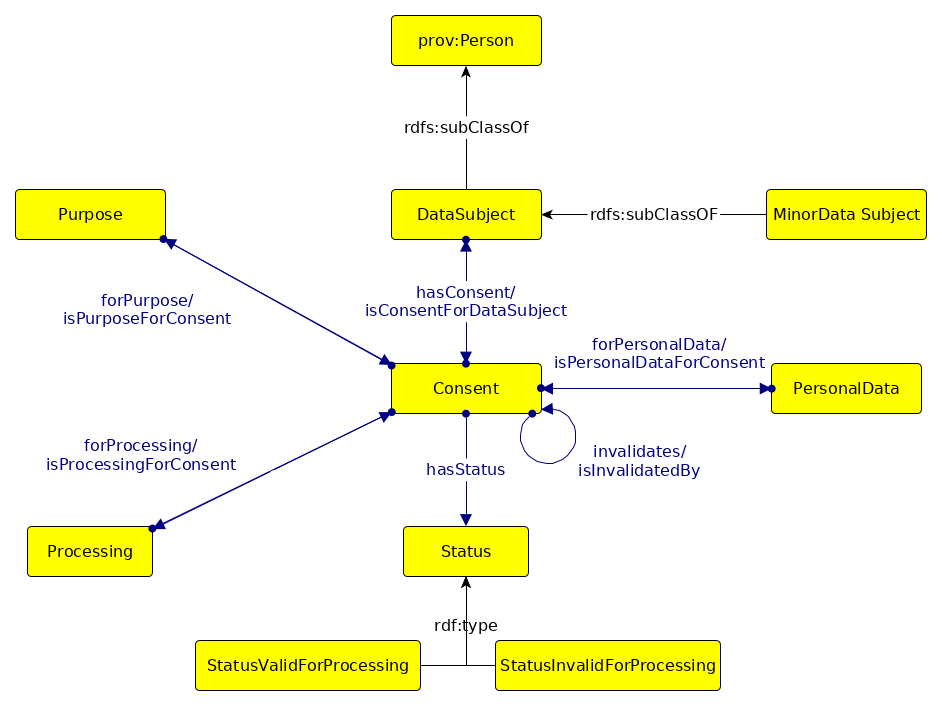
\includegraphics[width=0.8\linewidth]{img/gconsent_core.png}
    \caption{Core concepts in GConsent \cite{pandit_gconsent_2019}}
    \label{fig:vocabs:gconsent-core}
\end{figure}

The \texttt{DataSubject} is the person the consent is associated with as an agreement of their choices. This person may or may not be the same entity that gave the consent - as in the case of parent or guardian giving consent for a child or the act of delegation. The \texttt{DataSubject} class is defined as a subclass of \texttt{prov:Person}, and has the subclass \texttt{MinorDataSubject} to denote a data subject that is legally a minor or a child.
Each instance of \texttt{Consent} is associated with one and only one \texttt{DataSubject}, and any further changes or modifications to the state of consent will continue to be associated with the same \texttt{DataSubject}.
The \texttt{PersonalData} is the set of personal data associated with the consent. Where multiple personal data are associated with a single instance of consent, it is interpreted to mean the union of these sets of personal data. Similarly, \texttt{Purpose} and \texttt{Processing} are also to be interpreted as union rather than intersection.
The `status' or `state' of consent indicates the suitability of using that specific instance of consent as a legal basis for the processing of personal data defined by the consent attributes.

\texttt{Purpose} and \texttt{Processing} are concepts that have semantic meaning based upon their use within the GDPR.
`Processing' is defined by Article 4-2, while `Purpose' has no specific definition provided but can be summarised as the intent or aim of why the set of personal data is needed or to be used for. In practice, purpose is generally defined at a higher abstract level, and often encompasses several types or categories of data. An example of this is a privacy policy specifying `account information' and `location of service use' - which are data categories, that are `collected' and `used' - which are processing operations on the personal data, `to ensure security of the account' - which is the purpose the personal data will be processed for. The relation between a purpose and its associated processing operations is quite opaque when considered as a purpose involving one or more processing operations. Based only on the description, it is difficult to determine which processing operations a purpose entails and vice versa, and their usage may not always be implied or commonly understood. Therefore, GConsent provides purpose and processing as self-declarative high-level concepts which can be extended with additional information for granularity and transparency.

\subsubsection{Context of Consent}
The context of consent refers to the attributes such as the location or time when the instance of consent was created, invalidated, generated, changed, modified, given, or recorded.
GConsent provides concepts for expressing location, medium, and timestamp to indicate instant of creation or invalidation along with capturing the `expiry' of consent as either a instant of time or a duration using the Time vocabulary \cite{cox_time_2017}. The context also represents how consent was `provided' by a Person or Data Subject or Delegation. 
The provided contexts in GConsent are visualised in \autoref{fig:vocabs:gconsent-context}.

Context is associated with an instance of consent using the generic property \texttt{hasContext}, with specialised properties extending it to indicate provision, expiry, location, time, and medium. 
Additional contexts can be represented and associated by extending \texttt{hasContext} in a similar manner.
\begin{figure}[htbp]
    \centering
    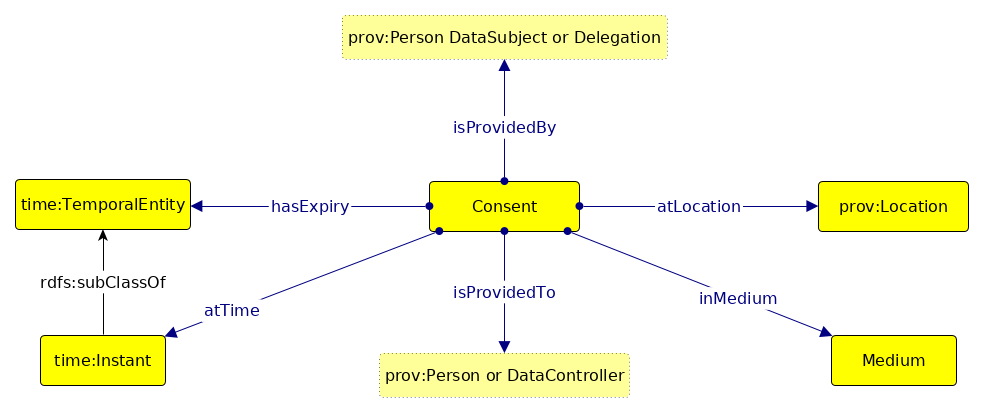
\includegraphics[width=0.8\linewidth]{img/gconsent_context.png}
    \caption{Concepts for representing context of consent in GConsent \cite{pandit_gconsent_2019}}
    \label{fig:vocabs:gconsent-context}
\end{figure}

\subsubsection{Consent States}
The state of consent determines the suitability of its usage as a legal basis in the processing of personal data.
From a compliance perspective, there are only two categories of states - one which permits legal processing of personal data, and the other being insufficient or prohibitive for  processing.
GConsent represents these using the concepts by sub-classing \texttt{Status} as \texttt{StatusValidForProcessing} and \texttt{StatusInvalidForProcessing} to indicate use of a consent instance as a valid or invalid legal basis as depicted in \autoref{fig:vocabs:gconsent-status}.
Instances provided to represent states of valid consent to indicate legal processing, and include - explicitly given, implicitly given, and given by delegation.
Instances provided that represent invalid states of consent to indicate processing should not be carried out include - unknown, not given, withdrawn, expired, invalidated, refused, and requested.

The use of state refers to tracking the consent of a data subject from the legal perspective, and is aimed to aid in the management of consent as an entity. For example, `unknown' reflects a situation where the status of consent is not known - which can occur when importing consent information data from another source.
This is distinct from `not given' which indicates an offer has been made for obtaining consent but the data subject has not yet provided any actionable response that could indicate acceptance or refusal - which are themselves represented by the states for `given' and `refused' respectively.
For meeting the obligations and requirements of GDPR compliance, it is not necessary to represent consent instances with states such as unknown or refused.
GConsent provides them based on the practical management of consent information where a Controller may wish to track the consent status of its processing operations throughout its life-cycle.
\begin{figure}[htbp]
    \centering
    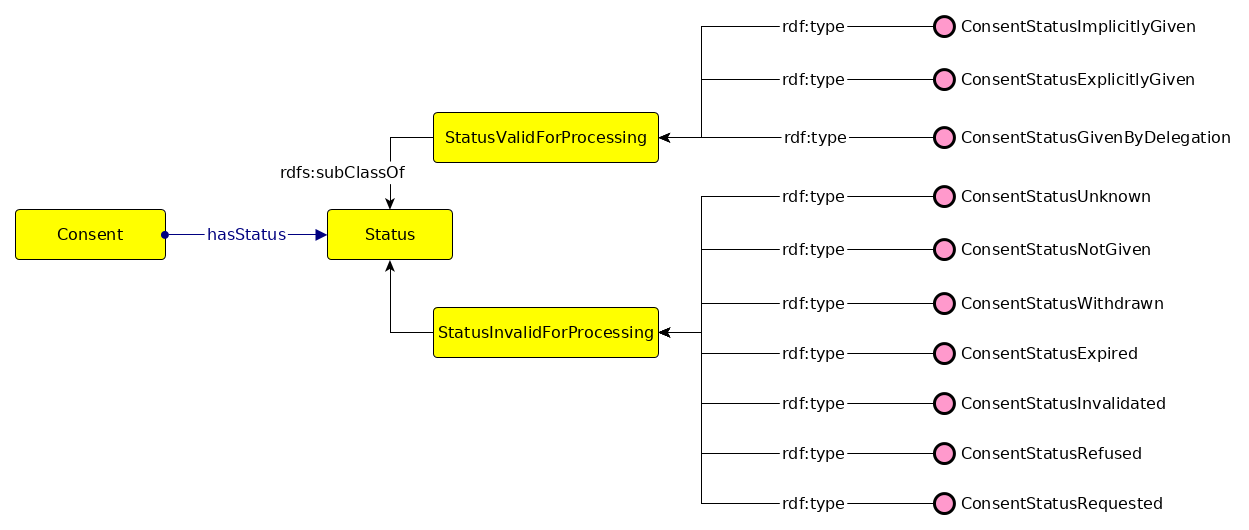
\includegraphics[width=\linewidth]{img/gconsent_status.png}
    \caption{Concepts representing state/status of consent in GConsent \cite{pandit_gconsent_2019}}
    \label{fig:vocabs:gconsent-status}
\end{figure}

GDPR requires keeping track of state change for consent - for example when the status changes from given to withdrawn or when the state if changed to invalidated because of the choice of the controller or some legal requirement. Whenever a consent status changes, this results in a new consent instance being created, which also assists in capturing the context of the new consent (such as time instant). This leads to a chain of consent instances, where the `latest' consent is at the `end' of this chain and indicates the most recent operation regarding consent states. It is vital to record such provenance to demonstrate past processing was in compliance with the state of consent at that point in time and to show the changes in consent as part of its life-cycle.

\subsubsection{Example Use-Case}
The documentation of GConsent provides example applications of the ontology in four use-cases to demonstrate how information can be represented, which are - (i) change in consent state, (ii) capturing given consent, (iii) capturing consent given via delegation, and (iv) capturing consent when data is shared with a third party.
The fourth use-case is presented here to demonstrate the application of GConsent and the use of its concepts to represent information towards GDPR compliance.

The example, visually represented in \autoref{fig:vocabs:gconsent-example}, shows association of a third party in the role of a data processor\footnote{Under GDPR, a processor is not considered a third party, but has its own defined role as an entity associated with the Controller. However, from a lay person's perspective, the individual is the first party, the Controller is the second party, and any other entity is a third party. GConsent reflects this use in its structuring of entities where a Processor is considered a special type (sub-class) of Third Party.}
with whom the data is shared for the purpose of advertising. The association is captured by the instance \texttt{ex:AdvertisingArrangement} of type \texttt{prov:Association}, and has \texttt{ex:AdPartner} defined as a \texttt{gdprov:Processor} defined with the role as \texttt{gdprtext:Processor}. It is also possible to list out the specific arrangement for this association using the \texttt{prov:hadPlan} property and a \texttt{gdprov:Process} instance to list out the specific steps and entities involved in the data sharing arrangement.

The example serves to demonstrate the practical use of GConsent in representing information about consent, where PROV-O is used to specify relationships with a Processor. GConsent can be combined or supplemented by other ontologies to define such associations and practical reflections of data sharing agreements between parties. The defined instance of consent in the example enables a Controller to track the state of consent as the data subject is provided with the choice of whether to agree to this arrangement or to refuse it, and where upon agreement the option to exercise the right to modify and withdraw the consent is also provided.
\begin{figure}[htbp]
    \centering
    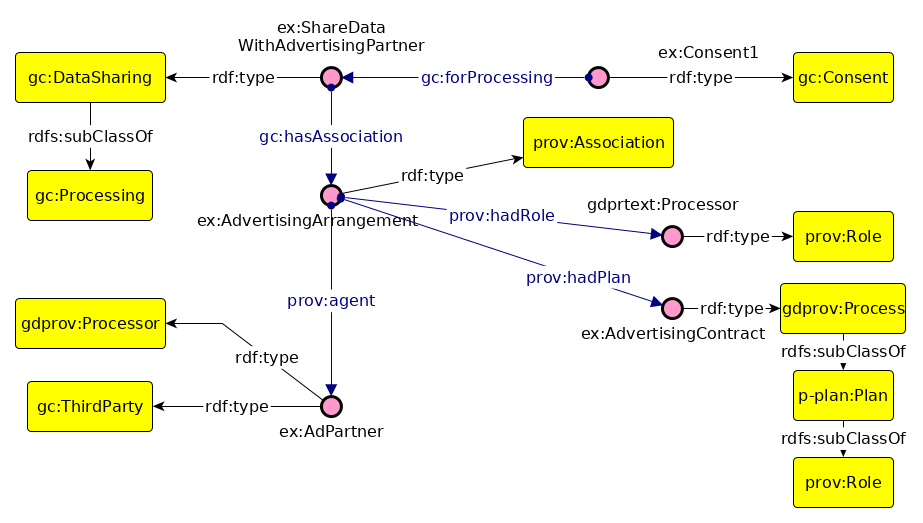
\includegraphics[width=0.8\linewidth]{img/gconsent_third_party_datasharing.png}
    \caption{GConsent representation of use-case involving third party data sharing \cite{pandit_gconsent_2019}}
    \label{fig:vocabs:gconsent-example}
\end{figure}

\subsection{Evaluation}\label{sec:voc:gconsent:evaluation}
GConsent as an ontology was evaluated regarding its capability to express information about consent using the methodology outlined in \autoref{sec:voc:methodology}.
This was an iterative process where the ontology was tested and modified to accommodate the requirements of the competency questions. Changes were made to the ontology where information was found to be missing or incorrectly modelled.
In particular, the iterations consisted of the degree and design of representing a dependency between purposes and processing operations associated with consent. These were ultimately rejected with the final iteration modelling purpose and processing independent of each other to provide greater granularity and reuse of these concepts.
GConsent was used and evaluated in the representation of consent information for a real-world website in the application of SHACL to validate information for GDPR compliance in \autoref{sec:testing:shacl}.

GConsent was published in the Extended Semantic Web Conference (ESWC) as a peer-reviewed publication \cite{pandit_gconsent_2019} in the Ontologies and Reasoning Track. As ESWC is a top-tier semantic web conference with a rigorous review process, the acceptance of GConsent demonstrates its contribution as a semantic web resource.
Along with this, the documentation of GConsent, available online, also provides extensive information about the ontology and its potential applications. It also provides a brief comparison of the ontology with relevant approaches within the state of the art.
GConsent, along with the Consent Receipt standard \cite{lizar_consent_2017}, had a direct impact on the design and development of consent information within the DPV. In particular, GConsent provided the concepts for expression of consent based on the GDPR and competency questions for integrating those with the rest of DPV.
As of February 2020, GConsent does not currently have any citations (excluding self-citations) given the recency of its publication.

\subsubsection{Fulfilment of Competency Questions}
The assessment of the extent to which GConsent provides concepts and relationships to answer the competency questions is presented in \autoref{table:gconsent:cq}. 
In these, the PROV-O and Time ontologies are used in conjunction with GConsent to represent provenance and temporal information about the consent and changes to it.
PROV-O is also used to capture the association and roles of entities in the activities associated with consent.
Based on these, GConsent satisfies the requirements of providing information for answering the compliance questions regarding consent and thus fulfils research objective $RO3(c)$.
\begin{table}[htbp]
\footnotesize
\centering
\rowcolors{1}{}{gray!10}
\begin{tabularx}{\textwidth}{|p{1cm}|X|p{4cm}|p{3.5cm}|}
\caption{Concepts and relationships in GConsent for answering competency questions} \\ \hline
\label{table:gconsent:cq}
\textbf{CQ} & \textbf{Question} & \textbf{Concepts} & \textbf{Properties} \\ \hline
\multicolumn{4}{|l|}{\textbf{Questions about consent}} \\ \hline
\textit{CMQ35} & Who is the consent about? & \textit{DataSubject} & \textit{isConsentForDataSubject} \\ \hline
\textit{CMQ36} & What type of Personal Data are associated with the Consent? & \textit{PersonalData} & \textit{forPersonalData} \\ \hline
\textit{CMQ37} & What type of Purposes are associated with the Consent? & \textit{Purpose} & \textit{forPurpose} \\ \hline
\textit{CMQ38} & What type of Processing are associated with the Consent? & \textit{Processing} & \textit{forProcessing} \\ \hline
\textit{CMQ39} & What is the Status of Consent? & \textit{Status} & \textit{hasStatus} \\ \hline
\textit{CMQ87} & Is the current status valid for processing? & \textit{StatusValidForProcessing, StatusInvalidForProcessing} & \textit{hasStatus} \\ \hline
\textit{CMQ46} & Who is the consent given to? & \textit{prov:Person, DataController} & \textit{isProvidedTo} \\ \hline
\multicolumn{4}{|l|}{\textbf{Questions about how the consent was created/given/acquired/changed/invalidated}} \\ \hline
\textit{CMQ42, CMQ76} & Who created/gave/acquired/invalidated the consent? & \textit{DataSubject, Delegation} & \textit{isProvidedBy} \\ \hline
\textit{CMQ41, CMQ77} & If consent was created/gave/acquired/invalidated through Delegation, who acted as the Delegate? & \textit{prov:Person, Delegation} & \textit{prov:agent} \\ \hline
\textit{CMQ43} & If consent was created/gave/acquired/invalidated through Delegation, what was the role played by Delegate? & \textit{prov:Role} & \textit{prov:hadRole} \\ \hline
\textit{CMQ44} & If consent was created/gave/acquired/invalidated through Delegation, how was the delegation executed? & \textit{prov:Activity} & \textit{prov:hadActivity} \\ \hline
\multicolumn{4}{|l|}{\textbf{Questions about the context of how consent was created/gave/acquired/invalidated}} \\ \hline
\textit{CMQ53, CMQ84} & What is the location of associated with consent? & \textit{prov:Location} & \textit{atLocation} \\ \hline
\textit{CMQ54, CMQ85} & What is the medium associated with consent? & \textit{Medium} & \textit{inMedium} \\ \hline
\textit{CMQ55, CMQ86} & What is the timestamp associated with the consent? & \textit{time:Instant} & \textit{atTime} \\ \hline
\textit{CMQ56, CMQ87} & What is the expiry of the consent? & \textit{time:TemporalEntity} & \textit{hasExpiry} \\ \hline
\textit{CMQ82} & What artefacts were shown when consent was acquired/changed/created/invalidated? & \textit{prov:Entity} & \textit{prov:used} \\ \hline
\multicolumn{4}{|l|}{\textbf{Questions related to Third Party associated with the consent}} \\ \hline
\textit{CMQ57} & Is the purpose or processing associated with a third party? & \textit{prov:Association}, \textit{ThirdParty} & \textit{hasAssociation, prov:agent} \\ \hline
CMQ58 & What is the role played by the third party in the purpose or processing? & Role & prov:hadRole \\ \hline
\end{tabularx}
\end{table}

\subsubsection{Comparison with SotA}
The existing approaches regarding consent were presented and analysed in \autoref{sota:analysis:consent}, with the observation about the lack of approaches modelling consent as required for GDPR compliance.
\autoref{table:gconsent:sota} demonstrates a comparison of GConsent with the SotA based on the attributes used in this analysis.
The column headings indicate the representation of information within an approach and are abbreviated to indicate - Personal Data (PD), Purpose (Pu), Processing (Pr), Data Sharing (Sh), Data Storage (St), Recipients (Rp), Data Source (S), Withdrawal of consent (W), Delegation (D), Visualisation (V), Significant effects of processing (SE), (Ct): Context (Ct), Types or States (T).
A check mark (\cmark) indicates the approach provides or models that information category, and a blank cell indicates that the approach does not provide representation for that information or that there is no open and public information available regarding its provision.
\begin{table}[htbp]
\footnotesize
\centering
\rowcolors{1}{}{gray!10}
\begin{tabularx}{\textwidth}{|l|X|X|X|X|X|X|X|X|X|X|X|X|}
\caption{Representation of consent in SotA}\label{table:gconsent:sota} \\
\hline
\textbf{Work} & \textbf{PD} & \textbf{Pu} & \textbf{Pr} & \textbf{Sh} & \textbf{St} & \textbf{Rp} & \textbf{S} & \textbf{W} & \textbf{D} & \textbf{SE} & \textbf{Ct} & \textbf{T} \\ \hline
\rowcolor[gray]{0.8}
GConsent & \cmark & \cmark & \cmark & \cmark & \cmark & \cmark & \cmark & \cmark & \cmark & \cmark & \cmark & \cmark \\ \hline
SPECIAL & \cmark & \cmark & \cmark & \cmark & \cmark & \cmark &  & \cmark &  &  &  &  \\ \hline
SPL+CitySPIN & \cmark & \cmark & \cmark & \cmark & \cmark & \cmark &  & \cmark &  &  &  &  \\ \hline
Lodge et al & \cmark & \cmark &  &  &  &  &  &  &  &  &  &  \\ \hline
Peras & \cmark & \cmark & \cmark & \cmark & \cmark &  &  & \cmark &  &  &  &  \\ \hline
Coletti et al & \cmark & \cmark &  &  &  &  & \cmark & \cmark &  &  &  &  \\ \hline
AdvoCATE & \cmark & \cmark &  &  & \cmark & \cmark &  &  &  & \cmark & \cmark &  \\ \hline
RestAssured & \cmark & \cmark & \cmark & \cmark & \cmark & \cmark &  &  &  &  &  &  \\ \hline
OPERANDO & \cmark & \cmark & \cmark & \cmark &  & \cmark &  &  &  &  &  &  \\ \hline
PoSEID-on & \cmark &  &  &  &  & \cmark &  &  &  &  &  &  \\ \hline
MHMD & \cmark &  &  &  &  &  &  &  &  &  &  &  \\ \hline
DECODE & \cmark & \cmark &  &  & \cmark &  &  &  &  &  &  &  \\ \hline
Consent Receipt & \cmark & \cmark &  &  &  &  &  &  &  &  & \cmark & \cmark \\ \hline

\end{tabularx}
\end{table}

The table demonstrates the contribution of GConsent to the state of the art. 
Compared to the SotA, GConsent provides novel contributions for the representation of consent for GDPR compliance and thus extends the state of the art.
In particular, the depiction of delegation is more detailed and provides representation of information based on compliance requirements of GDPR.
As the table depicts, GConsent is currently the only approach that models delegation based on its potential relevancy to the evaluation of GDPR compliance.
GConsent is also novel in the provision of consent states which enable documenting of information from a controller's perspective regarding the evolution of consent throughout its life-cycle. This is useful for the management of consent as an entity in an information management system such as a database.
The SotA usually limits the consent state to given or withdrawn without consideration to its other states within the life-cycle as an entity.

\subsubsection{Application to external use-case from SPECIAL project}\label{sec:gconsent:use-case:SPECIAL}
The use-case described in \autoref{sec:gdprov:use-case:SPECIAL} is used here to demonstrate the use and sufficiency of GConsent in management of consent information. The use-case concerns the scenario where a data subject named Sue gives consent to BeFit company for sharing her activity profile with other companies for receiving targeted ads. She later receives ads from a local Gym and investigates to find that the Gym is using her activity profile shared by BeFit - and that this activity is consistent with her previously given consent. She then withdraws her consent and asks both companies to delete her data.

The representation of this use-case using GConsent consists of using its concepts to represent the information, and to then utilise SPARQL to answer the queries - similar to the exercise in \autoref{sec:gdprov:use-case:SPECIAL} for GDPRov. \autoref{table:gconsent:use-case:SPECIAL} presents the concepts for representing the use-case using GConsent, GDPRov, and SPECIAL vocabularies. The corresponding RDF representation using GConsent is provided in \autoref{code:gconsent:use-case:special} with the queries for deriving answers to questions (i) - (iv) in the use-case are provided in \autoref{code:gconsent:use-case:special-sparql}.
\begin{center}
\scriptsize
\begin{tabularx}{\textwidth}{|p{0.3\linewidth}|X|X|X|}
\caption{GConsent concepts to represent external use-case from SPECIAL}\label{table:gconsent:use-case:SPECIAL} \\
\toprule
\textbf{Statement} & \textbf{GConsent} & \textbf{GDPRov} & \textbf{SPECIAL} \\
\midrule
\endhead
Sue & \texttt{DataSubject} & \texttt{DataSubject} & \texttt{DataSubject} \\ \hline
BeFit & \texttt{DataController} & \texttt{DataController} & \texttt{Controller} \\ \hline
Biomedical parameters, heart rate, calories consumption, activity profile & \texttt{PersonalData} & \texttt{PersonalData} & \texttt{Data} \\ \hline
Collect data & \texttt{Collection Of PersonalData} & \texttt{Data Collection Activity} & \texttt{Collect} \\ \hline
Provide feedback on activity & \texttt{Purpose} & \texttt{Purpose} & \texttt{Purpose} \\ \hline
Give consent (opt-in) & N/A & \texttt{Acquire Consent Activity} & \texttt{ConsentAssertion} \\ \hline
Targeted ads related to fitness & \texttt{Purpose} & \texttt{Purpose} & \texttt{Purpose} \\ \hline
Share data & \texttt{Sharing Of Personal Data} & \texttt{Data Sharing Activity} & \texttt{Recipient} \\ \hline
Gym & \texttt{ThirdParty} & \texttt{ThirdParty} & \texttt{Recipient} \\ \hline
Consent agreement & \texttt{Consent Status Explicitly Given} & \texttt{GivenConsent} & \texttt{LogEntryContent} \\ \hline
Delete data & \texttt{Deletion Of Personal Data} & \texttt{Data Deletion Activity} & N/A \\ \hline
Withdraw consent & N/A & \texttt{Withdraw Consent Activity} & \texttt{ConsentRevocation} \\ \hline
Withdrawn consent & \texttt{Consent Status Withdrawn} & N/A & N/A \\
\bottomrule
\end{tabularx}
\end{center}
\begin{listing}[htbp]
\begin{minted}{turtle}
# Entities
:Sue a gc:DataSubject .
:BeFit a gc:DataController .
:Gym a gc:ThirdParty .
# Personal Data
:Activity_Profile a gc:PersonalData .
# Purpose
:Targeted_ads_related_to_fitness a gc:Purpose .

# Sue gives consent to BeFit
:Consent1_registration a gc:Consent ;
	gc:isConsentForDataSubject :Sue ;
	gc:isProvidedToController :BeFit ;
	gc:forPurpose :Targeted_ads_related_to_fitness ;
	gc:forProcessing gc:CollectionOfPersonalData, 
		gc:ShareDataForTargetedAds ;
	gc:forPersonalData :Activity_Profile ;
	gc:hasStatus gc:ConsentStatusExplicitlyGiven .

# BeFit shares data with Gym 
# assumed similar 'policy' structure as SPECIAL
:ShareDataForTargetedAds a gc:DataSharing ;
	gc:involvesThirdParty :Gym .
	gc:sharesDataWithThirdParty :Gym .

:Consent_info_shared_by_BeFit_with_Gym a gc:Consent ;
	gc:isConsentForDataSubject :Sue ;
	gc:isProvidedTo :BeFit ;
	gc:forPurpose :Targeted_ads_related_to_fitness ;
	gc:forProcessing gc:UseOfPersonalData ;
	gc:forPersonalData :Activity_Profile ;
	gc:hasStatus gc:ConsentStatusExplicitlyGiven .	

# Sue withdraws consent
:Consent2_withdraw a gc:Consent ;
	gc:isUpdatedConsentFor :Consent1_registration ;
	gc:forPurpose :Targeted_ads_related_to_fitness ;
	gc:forProcessing gc:CollectionOfPersonalData, 
		gc:ShareDataForTargetedAds ;
	gc:forPersonalData :Activity_Profile ;
	gc:hasStatus gc:ConsentStatusWithdrawn .

\end{minted}
\caption{GConsent representation of external use-case from SPECIAL}
\label{code:gconsent:use-case:special}
\end{listing}
\begin{listing}[htbp]
\begin{minted}{sparql}
# Query (i)
# retrieves :Activity_Profile as data shared for Sue
# queried over Gym's records
SELECT ?personal_data
WHERE {
	?_ gc:isConsentForDataSubject :Sue .
	?_ gc:forPersonalData ?personalData .
}

# Query (ii)
# retrieves :BeFit as data source
# retrieves :Targeted_ads_related_to_fitness as purpose
# queried over Gym's records
SELECT ?party, ?purpose {
	?_ gc:isConsentForDataSubject :Sue .
	?_ gc:forPersonalData :Activity_Profile .
	?_ gc:isProvidedTo ?party .
	?_ gc:forPurpose ?purpose .
}

# Query (iii)
# retrieves :CollectionOfPersonalData as the processing operation
# from which it needs to be inferred that data is collected from Sue
# queried over BeFit's records
SELECT ?data_processing {
    ?_ gc:forPersonalData :Activity_Profile .
    ?_ gc:forProcessing ?data_processing .
}

# Query (iv)
# retrieves :Consent1_registration as satisfying
# conditions for data sharing with Gym
# queried over BeFit's records
SELECT ?consent
WHERE {
	?consent a gc:Consent .
	?consent gc:isConsentForDataSubject :Sue .
	?consent gc:forPersonalData :Activity_Profile .
	?consent (gc:forProcessing/gc:sharesDataWithThirdParty) :Gym .
}


\end{minted}
\caption{SPARQL queries using GConsent for external use-case from SPECIAL}
\label{code:gconsent:use-case:special-sparql}
\end{listing}

From the above representation and queries, the use of GConsent demonstrates the use of terms (purpose, sharing, etc.) closer to those of SPECIAL as compared to GDPRov's representation in \autoref{sec:gdprov:use-case:SPECIAL}.
At the same time, the inability to represent information about activities such as how the data was collected or shared is also evident since GConsent does not represent them while GDPRov does.
From a consent perspective, the consent `records' represented using GConsent are more clear and concise in terms of what the consent related to, and how it was withdrawn.
The above representation therefore demonstrates GConsent's use in managing consent information, with the SPARQL queries used to retrieve the answers to questions pertaining to use of Sue's personal data within the use-case.

\subsection*{Summary}
GConsent is an ontology for the representation of consent and its associated information for GDPR compliance. It fulfils the research objective $RO3(c)$ and along with GDPRov forms the second major contribution of this thesis.
GConsent has been published in a peer-reviewed publication and is available online as an open and reusable resource along with an extensive and descriptive documentation.

GConsent is currently the only approach within the state of the art to provide representations of attributes of consent and its states based on the requirements of the GDPR.
GConsent thus represents a novel representation of consent based on GDPR and provides the concept of states for practical management of consent information from a controller's perspective. It also provide detailed information representation regarding the context of consent which enables documenting information required for evaluating the validity of consent under GDPR compliance requirements.

% DPV
\section{Data Privacy Vocabulary (DPV)}\label{sec:voc:DPV}
The Data Protection Vocabulary \cite{pandit_creating_2019} is a semantic web ontology for representing information about personal data handling based on legal requirements such as those for GDPR compliance.
It is the outcome of work done by the W3C Data Privacy Vocabularies and Controls Community Group (DPVCG) which consists of collaboration between a community of academics, researchers, industry stakeholders, and legal experts as initially described in \autoref{sec:intro:dpvcg}.
The DPVCG aims to work towards establishment of interoperable standards regarding representing information about personal data processing for which there are currently no existing standards.

The DPVCG was initiated as an outcome of the SPECIAL project \cite{pandit_d6.5_2019}, and therefore bears close association and alignment with the SPECIAL vocabularies.
In particular, the SPECIAL core vocabulary was used as the basis to create the DPV core vocabulary, providing compatibility between the DPV and SPECIAL vocabularies and frameworks.

The DPV reflects a community consensus in its representation of information regarding data protection and personal data processing. While being a generic vocabulary, much of its design is based on and reflected by the requirements of the GDPR. The DPV, and by extension the DPVCG, reflect an ongoing effort to provide practical and useful semantic representations of information in an open and interoperable machine-readable form. 

\subsection{Relevance of DPV to this thesis}
The ontologies presented in this thesis as research contributions - namely GDPRtEXT, GDPRov, and GConsent - were part of the state of the art analysed by DPVCG in its methodology \cite{pandit_creating_2019}.
In addition, by being an active member of the DPVCG and a contributor in the creation of DPV, the author of this thesis has applied the experience of developing presented research to influence the design and modelling of information within the DPVCG.

The publication presenting DPV \cite{pandit_creating_2019} presents its creation methodology and concepts where the author of this thesis was a co-first author.
In addition to these, the vocabulary specification published online lists the author of this thesis as an co-editor and author of the ontology.
The deliverable D6.5 \cite{pandit_d6.5_2019} of the SPECIAL project presents the work of the DPVCG by describing the DPV based on the peer-reviewed publication of DPV \cite{pandit_creating_2019} and also features the author of this thesis as one of the lead authors within the deliverable.

Owing to the involvement of the author and the overlap between DPV and the research question and developed ontologies, the DPV is a research contribution influenced by the research presented in this thesis.
This section describes the DPV and compares it with the ontologies presented in this thesis to provide an extent of their overlap and provide the basis for comparison.
It demonstrates the differences in representation of information, scope, and methodology and their complimentary nature in representing information for GDPR compliance.

\subsection{Overview of DPV}
\subsubsection{Description of Data Privacy Vocabulary}
The DPV ontology is published at the W3C namespace \url{http://w3.org/ns/dpv} with its documentation and uses the namespace prefix \texttt{dpv}. 
The current iteration of vocabulary provides classes and properties to annotate and categorise information about legally compliant personal data handling. In this context, personal data handling refers to all operations associated with processing of personal data and its management including organisational measures which indirectly affect processing.

The DPV is a pseudo-modular ontology with a set of core concepts referred to as the `\textit{Base Ontology}' and modular extensions further expanding each concept in the form of a taxonomy. The base ontology represents the top-level classes for defining a policy of legal personal data handling.
The core concepts, visualised in \autoref{fig:vocabs:dpv-core}, consist of personal data category, processing, purpose, legal basis, data controller, recipient, data subject, technical and organisational measures, and the top-level concept of personal data handling which ties them together.

\begin{figure}[htbp]
    \centering
    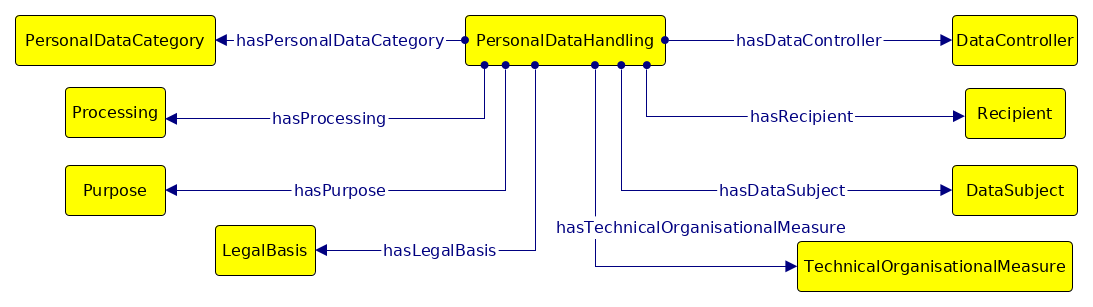
\includegraphics[width=\linewidth]{img/dpv-personaldatahandling.png}
    \caption{Core concepts in DPV \cite{pandit_creating_2019}}
    \label{fig:vocabs:dpv-core}
\end{figure}

\subsubsection{Personal Data Categories}
DPV uses the taxonomy provided by EnterPrivacy\footnote{\url{https://enterprivacy.com/wp-content/uploads/2018/09/Categories-of-Personal-Information.pdf}} to define a broad hierarchy of personal data categories based on the nature of information (financial, social, tracking) and to its inherent source (internal, external). 
In addition to these, the class \texttt{dpv:Special\-Category\-Of\-PersonalData} represents categories that are `special' or `sensitive' based on GDPR’s Article 9.

These personal data categories can be further extended by using the sub-class mechanism to depict specialised concepts such as `likes regarding movies'.
Sub-classing also enables representation of specific contexts such as derivation of personal data as represented by the class \texttt{dpv:DerivedPersonalData}.
This is useful to represent practical representation of personal data categories such as inference of opinions from social media.
Similar classes can be additionally added to specify contexts such as use of machine learning, accuracy, and source.
The aim of the providing such high-level concepts is to provide a sufficient coverage of abstract categories of personal data which can be extended using the subclass mechanism to represent concepts used in the real-world. 

\subsubsection{Purposes}
Purposes in DPV are organised hierarchically by using the sub-class mechanism to represent high-level and generic purposes of data handling.
Purposes provided in DPV include service provision, R\&D, commercial interest, security, service optimisation, and service personalisation. These are further extended to provide a total of 31 generic purposes.
These may be extended by further sub-classing to create more specific purposes as applicable to a scenario.
As GDPR requires a specific purpose to be declared in an understandable manner, specific purposes can be created using sub-classes of one or several \texttt{dpv:Purpose} categories to make them as specific to the use-case as possible.
 Purposes can be restricted to specific \texttt{contexts} using the class \texttt{dpv:Context} and the property \texttt{dpv:hasContext}.
Purposes can also be restricted to a specific \texttt{business sector} using the class \texttt{dpv:Sector} and the property \texttt{dpv:hasSector}.

\subsubsection{Processing Categories}
DPV provides a hierarchy of processing categories based on the requirements of regulations such as GDPR. 
DPV defines top-level classes to represent the following broad categories of processing - Disclose, Copy, Obtain, Remove, Store, Transfer, Transform, and Use.
Each of these are then again further expanded using sub-classes to provide 33 processing categories, which includes terms defined in the definition of processing in GDPR (Article 4-2).
The DPV provides properties with a boolean range to indicate the nature of processing regarding \texttt{Systematic Monitoring}, \texttt{Evaluation or Scoring}, \texttt{Automated Decision-Making}, \texttt{Matching or Combining}, \texttt{Large Scale processing}, and \texttt{Innovative use of new solutions} - as these affect assessment of legal data processing under GDPR.

\subsubsection{Technical and Organisational Measures}
GDPR Article 32 requires implementing appropriate measures by taking into account the state of the art, the costs of implementation and the nature, scope, context and purposes of processing, as well as risks, rights and freedoms.
These are represented as technical and organisational measures in the DPV.
Examples include pseudo-anonymisation and encryption of personal data, the ability to restore the availability and access to personal data in a timely manner in the event of a physical or technical incident, and a process for regularly testing, assessing and evaluating the effectiveness of technical and organisational measures for ensuring the security of the processing.
The generic property \texttt{dpv:measureImplementedBy} enables referencing the implementation measure as a comment or IRI.
The class \texttt{StorageRestriction} provides expression of measures used for storage of data with two specific properties provided for storage location and duration restrictions.

\subsubsection{Consent and Legal Bases}
DPV provides \texttt{dpv:LegalBasis} as a top-level concept to represent various legal bases that can be used for justifying processing of personal data.
The definition of a `legal basis' is based on the justification for processing which has a provision in the law. The concept itself is not based on any specific jurisdiction, but needs to be interpreted in terms of the legal bases defined and provided within the laws applicable within a jurisdiction.

For the GDPR, which is a EU specific law, and therefore is not binding in the interpretation of legal bases across all use-cases, the DPV provides the legal bases specific to GDPR as a separate aligned vocabulary under the \url{https://www.w3.org/ns/dpv-gdpr} and namespace (prefix: \texttt{dpv-gdpr}). 
This vocabulary defines the legal bases defined by Articles 6 and 9 of the GDPR to represent the legal justification of processing personal data.

Consent as a special case of legal basis provided by the GDPR is provided with additional properties and classes within the core DPV vocabulary to reflect the information requirements associated with its validity as a legal basis.
The concepts associated with consent provide terms to describe consent provision, withdrawal, and expiry.
The structure of these was adapted from an analysis of existing work in the form of Consent Receipt \cite{lizar_consent_2017} and GConsent \cite{pandit_gconsent_2019} with the intention to enable documenting attributes associated with consent which can demonstrate and evaluate its validity based on requirements of the GDPR.

\subsection{Comparing DPV with GDPRtEXT, GDPRov, and GConsent}
DPV has several commonalities with the ontologies presented in this thesis arising from the common aim of representing information for legal compliance with laws such as the GDPR.
However, the aim and granularity of representing information about all attributes relevant to the processing of personal data differentiates the DPV from the specific focus of ontologies presented in this thesis.
Given the high-level and abstract nature of DPV in its concepts, and the more granular and representative focus of developed ontologies, there is a possibility of aligning or combining the two.
While there have been no efforts to carry out an exercise to combine or align the developed ontologies with DPV, their comparison as presented here demonstrates the possibility and applicability of such an approach.

\subsubsection{Representing information about GDPR concepts}
GDPRtEXT provides a linked data version of GDPR and a SKOS glossary of concepts associated with GDPR compliance, which can be used to link information to the clauses and concepts of GDPR.
This has been used by GDPRov and GConsent to define the source of its concepts within the text of GDPR.

The DPV, whose concepts represent generic legal terms, does not link its concepts to the GDPR except in cases where the defined concept was directly taken from the definition provided by GDPR.
In such cases, it uses the URI format prescribed by the EU Publications Office to indicate the specific clause of GDPR. The URI format\footnote{The format is based on using templates to indicate the alphanumeric characters of articles and clauses. The template format can be represented as: \texttt{https://eur-lex.europa.eu/eli/reg/\{year\}/\{number\}/art\_\{X\}/par\_\{X\}/pnt\_\{X\}/oj}}, similar in its structuring of contents with GDPRtEXT, is based on an upcoming iteration\footnote{The information is based on a private communication between the author of the thesis with members of the EU Publications Office. The prescribed IRI, while not officially published or documented, currently resolves to the web-page of the legislation, which in this case is the GDPR.} of the ELI vocabulary which will be used in all EU published legislations to offer granular linking to their clauses.
Since the format prescribed by EU Publications Office is authoritative in its nature, the links provided by GDPRtEXT need to be aligned or replaced with those defined using the newer ELI format which offers further advantages in provision of concepts and granularity.

One of the aims of the DPVCG is to provide a glossary of concepts associated with legal personal data handling. For this, the concepts of DPV itself can be considered as a glossary of terms, though not defined as such within the ontology. This use of `glossary' refers to providing the concepts to an adopter in order to represent the required information. Since these terms do not necessarily arise from a particular legislation, their sources are based more on their use as a commonly understood concept or notion within the legal domain.
In terms of coverage, GDPRtEXT focuses more on terms directly obtained through the text of the GDPR while the DPV focuses on the modelling of concepts based on their relevance to defining personal data handling.
Therefore, while there is a small overlap in the concepts directly associated with GDPR, the two vocabularies differ in the provision and definition of terms. For example, GDPRtEXT defines \texttt{DataSecurity} based on Article 28 and 32 of the GDPR as obligations for Controllers and Processors, while DPV defines \texttt{Security} as a purpose. To further exemplify this distinction, DPV aims to offer terms that reflect real-world practices while GDPRtEXT focuses on the legal text of GDPR. This is evident from the hierarchical taxonomy of concepts in DPV, such as for personal data categories and purposes, so as to enable modelling of practices across a broader spectrum of use-cases.

\subsubsection{Representing information about activities}
The DPV does not provide representation of activities through which it can be compared with GDPRov.
Instead, DPV provides concepts to represent `processes' taking place within an organisation, such as those for ensuring technical and organisational measures, purposes, and processing.
The modelling of an instance of personal data handling, which consists of specifying the purpose, processing, and technical \& organisational measures, can be compared with the modelling of plans in GDPRov where a purpose represents a plan and its steps represent processing activities - which can be further annotated with measures and legal bases.
Through this, it can be summarised that the focus of GDPRov is on representing the activities with granularity in terms of their composition and dependency, and that of DPV is on providing metadata as an overview of  the processing and data handling practices. With this, it is possible to define an instance of personal data processing using DPV to indicate the high-level summary of associated information and further expand it using GDPRov to represent details of processes and capture their provenance in ex-ante/ex-post phases.

\subsubsection{Representing information about consent}
The DPV and GConsent both provide concepts to represent information about consent based on the requirements specified by GDPR.
In this, both share the aim to document the context of consent with a view towards establishing its validity and compliance.
The difference between the two is based on the granularity and use of existing vocabularies to represent this information.

The DPV utilises the model provided by its core or base vocabulary to represent information by specifying consent as the legal base used to justify processing of personal data.
In addition to this, it provides properties to indicate the specific notice displayed to obtain consent, its expiry, the obtaining or provision of consent, and its withdrawal.
In this, attributes such as timestamp, method used to carry out the provision and withdrawal are used to indicate information regarding how the consent was obtained.
This is based on notion of providing a form of the Consent Receipt based on requirements of the GDPR.

The DPV does not prescribe or utilise any existing vocabulary to specify information.
In contrast, GConsent provides similar concepts as the DPV base vocabulary and uses vocabularies of PROV-O and GDPRov to represent the information about activities.
Given that GConsent was an input to the DPV and by extension influential in its modelling of consent, there is a degree of compatibility between the two based on the similarity of concepts.
In this, GConsent is a more detailed vocabulary while DPV provides a minimal set of concepts regarding consent but is more expressive in representing the overall information regarding data processing.

\subsection{Comparing DPV with SotA}\label{sec:voc:dpv-sota}
This sections compares the DPV with approaches presented in the SotA in \autoref{chapter:sota}.
The aim of this exercise to demonstrate the extent of DPV's contributions and presents its relation with the rest of approaches in SotA.
Since the DPV is not presented as a direct contribution of this thesis, its evaluation is not within the scope of this thesis.

The aim of the DPV as established by the DPVCG is providing a vocabulary for personal data handling which concerns representation of information relevant for legal compliance - in this case associated with GDPR. Based on this, the DPV is a vocabulary useful towards representing the state of processing rather than a framework or methodology that can be used to evaluate compliance.
Currently, the DPV is not accompanied by any documentation demonstrating its use or application in use-cases, with such activities planned in the future.

Comparing the DPV with other vocabularies in the SotA, the DPV provides a large amount of concepts as a top-down modelled taxonomy which can be expanded with additional concepts. This enables it to be adapted and expanded within any use-case, while the drawbacks of this are that it cannot be readily used in its current state.
This aspect of the DPV is novel within the SotA as no other approach aims to provide a similar taxonomy of concepts, and does not incorporate the requirements of extending it for a given use-case such as through the sub-classing mechanism.

The DPV base vocabulary provides a compact structure representing personal data handling which aims to represent all the relevant information required to evaluate and demonstrate compliance.
In this, it bears resemblance to the SPECIAL core vocabulary \cite{bonatti_special_2018-2} given that the DPVCG was an extension of SPECIAL's work on its vocabularies.
This approach is more suitable for representation or documentation of information from a compliance perspective, and is not intended to be specific to any particular law - though the GDPR clearly has a significant influence on the vocabulary.
This is again in contrast to the approaches in SotA which are often intended to be applied to a particular legislation and a specific use-case.

The representation of technical and organisational measures is the most distinctive feature of DPV, as currently no other approach within the SotA provides concepts to represent these.
While there have been efforts to establish vocabularies regarding specification and representation of privacy policies, these tend to focus on the use of concepts such as purpose, processing, data storage, data sharing, third parties - which have been utilised quite commonly in SotA.

\section*{Chapter Summary}
The chapter presented the ontologies created to fulfil the research objective $RO3$ along with the methodology used for their development and their evaluation. It also provides a comparison of the ontologies with related approaches of the SotA presented in \autoref{chapter:sota}.

The ontology engineering process was presented in \autoref{sec:intro:ontology-engineering} and described the methodology used for creating ontologies based on best-practices and guidelines advocated by the community. This included ensuring ontology quality, documentation, and releasing developed resources under an open and permissive license.
It also described utilisation of compliance questions presented in \autoref{sec:info:compliance-questions} as competency questions.

The presented ontologies consisted of GDPRtEXT, GDPRov, and GConsent.
GDPRtEXT, presented in \autoref{sec:voc:GDPRtEXT}, provides a linked data version of the text of GDPR created by extending the official ELI \cite{ELI_2012} ontology to represent its granular clauses. It also presents a SKOS glossary of concepts associated with GDPR compliance. GDPRtEXT enables the association and linking of information with the concepts and text of GDPR through the use of persistent IRIs. It thus fulfils research objective $RO3(a)$. GDPRtEXT extends the state of the art by providing an ELI-compatible extension capable of representing GDPR clauses at a granular level. It is also novel in providing a glossary of concepts associated with GDPR compliance.

GDPRov provides an OWL2 ontology for representing activities associated with personal data and consent in ex-ante and ex-post phases. It is presented in \autoref{sec:voc:GDPRov}.
The ontology is based on extending the existing ontologies of PROV-O \cite{lebo_prov-o_2013} and P-Plan \cite{garijo_p-plan_2014} with GDPR terminology using GDPRtEXT to represent activities in context of compliance requirements. GDPRov is novel in the use of PROV-O and P-Plan together based on the scientific workflow model to represent processes for GDPR compliance.
It provides an extensible model that can be used for representing processes related to compliance that can be extended for representing related  processes such as compliance activities and organisational processes.
The use of GDPRov enables capturing the provenance of plans or snapshots of a system at a given time and document them as evidence of planned and maintained compliance.
The use of P-Plan with PROV-O enables associating execution of activities with their intended planning and thereby provides systematic linking of ex-ante and ex-post compliance information.
GDPRov thus fulfils the research objective $RO3(b)$.

The representation of consent is provided by GConsent - an OWL2 ontology presented in \autoref{sec:voc:GConsent} that fulfils research objective $RO3(c)$.
GConsent provides representation of information relevant for evaluation of consent under GDPR obligations and requirements.
It extends on the notion of consent as an provenance entity in GDPRov and models the life-cycle of consent based on the concept of states.
State or status of consent reflects its suitability for use as a legal basis for processing and is modelled based on the management of consent information from an organisation's perspective. In this GConsent is novel within the SotA.
GConsent is also novel in the provision of concepts related to consent for the GDPR as it provides a more detailed and comprehensive vocabulary for representing information regarding consent.

The chapter also presented the DPV vocabulary published by the W3C Data Privacy and Vocabularies Community Group (DPVCG). The author of the thesis was an active contributor to the DPV, and subsequently the DPV shares its aim and bears similarity to the research presented in this thesis. \autoref{sec:voc:DPV} provides a summary of the DPV and compares it with the ontologies presented as contributions in this thesis, namely GDPRtEXT, GDPRov, and GConsent. A comparison of DPV with the SotA is also provided.
The DPV is intended to provide a vocabulary for representing information about personal data handling, and is not limited to the GDPR though it is influenced by it. It reflects a community consensus and is intended to be standardised, thereby providing a basis for its adoption.

Through these developed ontologies and the significance of the DPV, the primary problem guiding this research and outlined in the beginning of this thesis (\autoref{sec:intro:background}) of representing information and associating it with the GDPR has been addressed.
In the next chapter, the use of semantic web technologies to query this information to answer the compliance questions, such as those presented in \autoref{sec:info:compliance-questions}, is presented. The chapter also presents the use of semantic web technologies in validating information to ensure its correctness for assessing GDPR compliance based on constraints presented in \autoref{sec:info:constraints}.
The querying and validation of information are presented as minor contributions of the thesis, and satisfy the research objectives $RO4$ and $RO5$.
They utilise real-world use-cases to demonstrate application of the developed ontologies of GDPRtEXT, GDPRov, and GConsent to represent, query, and validate information for GDPR compliance.

% \chapter{Querying and Validating Information for GDPR Compliance}
\label{chapter:testing}
% chapter introduction
This chapter presents the application of semantic web technologies to query and validate information for GDPR compliance.
It represents information using the developed vocabularies of GDPRtEXT, GDPRov, and GConsent presented in \autoref{chapter:vocabularies}.
The queries are represented using SPARQL - a W3C standard for querying RDF - and are based on the compliance questions presented in \autoref{sec:info:compliance-questions}.
Validation is carried out based on the identified assumptions and constraints presented in \autoref{sec:info:constraints} and is expressed using SHACL which is the W3C standard for representing constraints.
The presented work represents minor contributions of this thesis, and fulfils the research objective $RO4$ regarding querying of information and $RO5$ regarding validation of information for GDPR compliance.

\autoref{sec:testing:sparql} presents the use of SPARQL to query information for answering compliance questions.
The use of SHACL to validate information for GDPR compliance is presented in \autoref{sec:testing:shacl}.
The chapter ends with conclusions drawn from the research in terms of novelty of contributions in \autoref{sec:testing:conclusion}.

\section{Querying Information for GDPR Compliance using SPARQL}\label{sec:testing:sparql}
This section presents the creation and utilisation of SPARQL queries to retrieve information relevant for GDPR compliance.
The creation of the queries is dependant on the ontological representation of information being retrieved, which in this case includes the use of GDPRov and GDPRtEXT ontologies. This is further explained in \autoref{sec:testing:sparql:relation}
A GDPR preparation guide published by the Irish Data Protection Commission was used as the source of compliance questions for which corresponding the SPARQL queries were created. The methodology used for this is presented in \autoref{sec:testing:sparql:methodology} with an demonstration of the developed queries presented in \autoref{sec:testing:sparql:demo}.
A note on the evaluation of this work is presented in \autoref{sec:testing:sparql:evaluation}.

\subsection{SPARQL queries and ontological representation of information}\label{sec:testing:sparql:relation}
The research regarding querying presented here is based on the task of retrieving information for answering questions relevant to the assessment of compliance.
It represents utilisation of technical solutions to automate the task of information retrieval and requires machine-readable data (or metadata).
For this, the developed vocabularies provide the ontological concepts and relationships necessary to express the information using GDPR terminology and enable the association of information with clauses and concepts of GDPR.

The compliance questions, as presented in \autoref{sec:info:compliance-questions}, do not use a specific ontology or vocabulary but instead are based in the natural language and use legal terminology. In order to utilise technological solutions for answering them, it is necessary to first convert these questions into queries which can be executed over the compliance representation.
Since the work presented in this thesis derives motivation from the use of semantic web technologies which use RDF for representing information, the task of querying utilises the SPARQL standard to retrieve this information.

The ontology used in the SPARQL queries must match the ontology used in the representation of information associated with compliance. Differences in ontologies would hamper the effective of execution of queries and have the potential to return invalid results or empty results.
The creation of SPARQL queries is therefore specific to the ontologies used in a particular information representation, and is therefore also specific to the use-case it is used in.

\subsection{Methodology}\label{sec:testing:sparql:methodology}
The methodology used for creation of SPARQL queries is based on utilisation of GDPRov to represent the concepts and GDPRtEXT to link the information to the GDPR.
The SPARQL queries thus created aim to retrieve information relevant to answering the question rather than present an evaluation or assessment of compliance.
While the compliance questions presented in \autoref{sec:info:compliance-questions} provide a basis for construction of semantic queries using SPARQL, we focused on identifying a real-world use-case of the use of such compliance questions to provide a demonstration of the application of this research.

\subsubsection{Utilising compliance questions from GDPR readiness guide published by DPC}
We utilised the guide titled ``Preparing Your Organisation for the GDPR – A Guide for SMEs'' published by Data Protection Commission of Ireland (DPC) as the basis for compliance questions which were represented using SPARQL as semantic queries.
The guide was published by the DPC in 2017 to help organisations in assessing their readiness towards GDPR compliance requirements.
It is accessible online\footnote{\url{http://gdprandyou.ie/wp-content/uploads/2017/12/A-Guide-to-help-SMEs-Prepare-for-the-GDPR.pdf}} and consists of a `table' (see  \autoref{fig:sparql:guide}) containing questions regarding information about an organisations processing activities.
The guide divides the questions into contextual sections based on addressing specific GDPR articles and obligations.
\begin{figure}[htbp]
\centering
\fbox{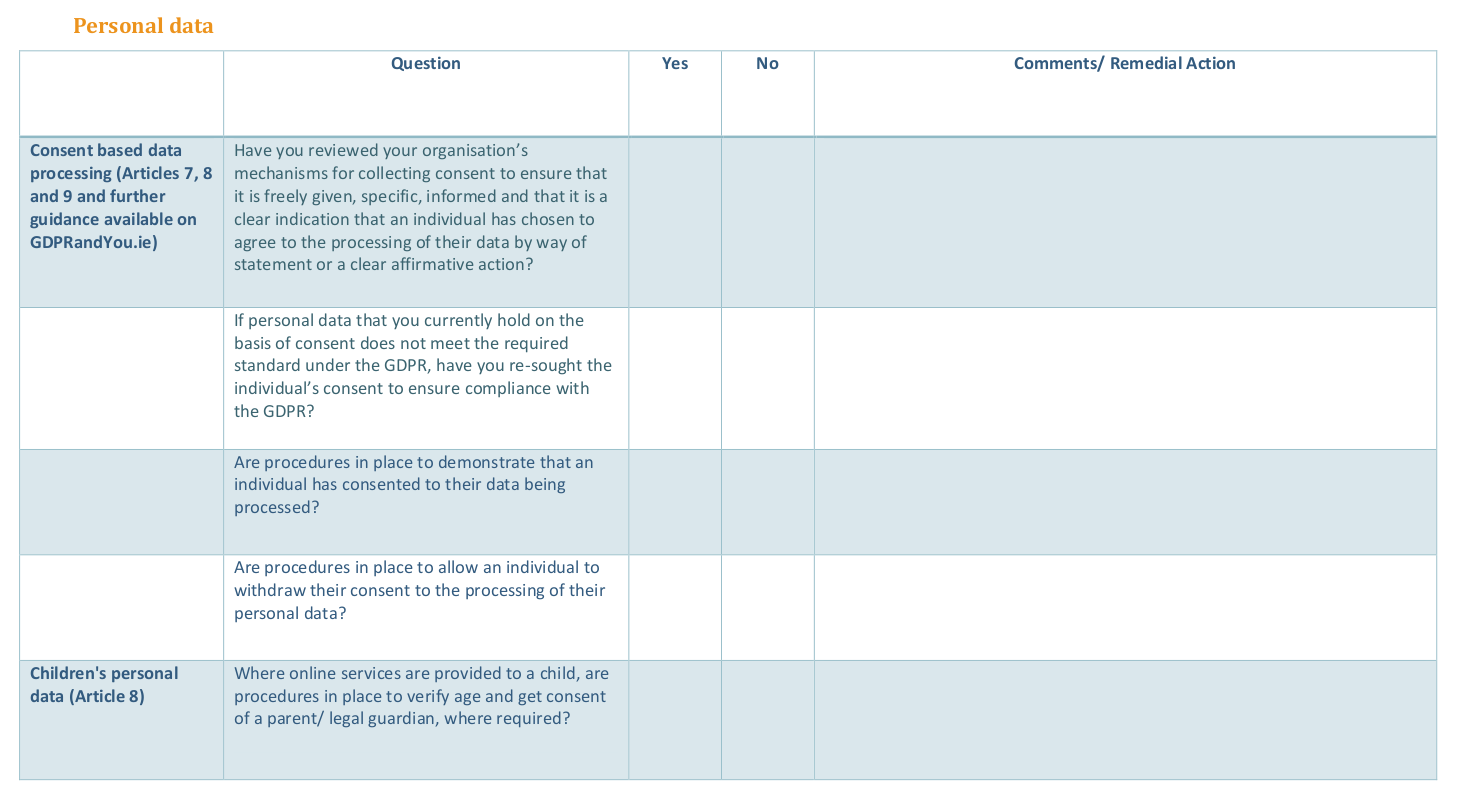
\includegraphics[width=\textwidth]{img/GDPR_guide_page_10.png}}
\caption{Questions for information required to assess compliance - Page 10 of ``Preparing Your Organisation for the GDPR - A Guide for SMEs'' published by Ireland's Data Protection Commission}
\label{fig:sparql:guide}
\end{figure}

\subsubsection{Steps of the methodology}
The steps followed in utilising the questions in the guide to create SPARQL queries and demonstrate their application were as follows:
\begin{enumerate}
    \item Analyse questions within the document to identify corresponding concepts and relationships in GDPRov and GDPRtEXT (see below). The questions largely concerned details of processing activities and organisational practices and therefore did not require use of GConsent.
    \item Represent questions as SPARQL queries using GDPRov and GDPRtEXT (see below)
    \item Create a synthetic use-case based on processing of personal data with GDPRov and GDPRtEXT used to represent information (see \autoref{sec:testing:sparql:demo})
    \item Execute SPARQL queries over use-case to retrieve answers for compliance questions (see \autoref{sec:testing:sparql:demo})
    \item Evaluate the queries based on the subjective criteria of - a) Extent of answering compliance questions b) Suitability of retrieved results in answering compliance questions (see \autoref{sec:testing:sparql:evaluation})
\end{enumerate}

\subsubsection{Analysis of GDPR Readiness Guide}
The guide contains 63 questions across 13 pages that are presented in 9 sections.
Its analysis consisted of categorising the questions based on requirements of information, relation to phases of compliance, and whether they were suitable to be implemented as SPARQL queries.
The analysis was recorded and published online\footnote{\url{https://w3id.org/GDPRep/checklist-demo/notes}} in the form of a spreadsheet with comments describing the thought process in interpreting each question's information requirements.

The first set of questions on page 1 concern consent and personal data and are structurally different than the other set of questions in that they are more abstract and generic and concern the overall practices concerning processing of personal data by the organisation.
These questions are described under the `general' category with other groups of questions having their category mentioned explicitly within the document.
Questions in the general category require information and practices associated with consent and personal data. Other categories contain questions which enquire explicitly about activities and mechanisms regarding compliance to specific obligations.

The questions were analysed and categorised into three categories based on their intended requirements towards information required for compliance. The three categories identified through this exercise were - demonstrative, evaluative, and assistive - based on the requirements of information associated with them. 
Demonstrative questions require answers that satisfy the compliance question and do not need further actions or processing based on the information. 
Assistive questions provide information that can be directly evaluated for compliance, with the term `assistive' indicating information that assists in the evaluation.
Evaluative questions retrieve information whose evaluation requires further information retrieved through additional questions based on the provided information.
The primary difference assistive and evaluative questions is whether they retrieve information which can be evaluated as is for compliance or whether it requires additional questions to retrieve further information.
These terms used for categorisation are arbitrary and do not relate to any specific methodology for legal compliance, but are useful to analyse the question from an information management perspective.

Questions were also analysed based on whether they relate to or require information regarding activities in ex-ante and ex-post phases.
The questions do not explicitly provide an indication of whether they enquire about a model of processing (ex-ante) or the execution (ex-post). The distinction was based on whether the question concerned information about practices, plans, or intentions regarding processing of personal data - in which case it was deemed to enquire about ex-ante information.
Similarly, if a question concerned past execution of activities or records of activities - it was said to enquire about ex-post information.
In some cases, questions were specified to enquire about both ex-ante and ex-post information based on potential application in both phases.

An overview of the questions is provided in \autoref{table:sparql:dpc-1}.
It assigns an ID for each question to enable associating it with the corresponding SPARQL query and for linking related questions in the analysis.
The column `\textit{Category}' reflects the category of question mentioned within the guide, with general used for the initial generic questions.
`\textit{Title}' refers to the title of the text within the guide, and the column `\textit{GDPR}' refers to an explicit mention of a GDPR clause within the question or its description.
\begin{center}
\footnotesize
\begin{tabularx}{\textwidth}{|l|l|X|l|}
\caption{Questions provided in the GDPR Readiness Guide} \label{table:sparql:dpc-1} \\
\toprule
\textbf{ID} & \textbf{Category} & \textbf{Title} & \textbf{GDPR} \\
\midrule
\endfirsthead

\caption*{Questions provided in the GDPR Readiness Guide (cont'd)} \\
\toprule
\textbf{ID} & \textbf{Category} & \textbf{Title} & \textbf{GDPR} \\
\midrule
\endhead

\multicolumn{4}{r@{}}{\footnotesize (Cont'd on following page)}\\
\endfoot

% \bottomrule
\endlastfoot

G1 & General & Categories of personal data and data subjects &  \\ \hline
G2 & General & Elements of personal data included within each data category &  \\ \hline
G3 & General & Source of the personal data &  \\ \hline
G4 & General & Purposes for which personal data is processed &  \\ \hline
G5 & General & Legal basis for each processing purpose (non-special categories of personal data) &  \\ \hline
G6 & General & Special categories of personal data &  \\ \hline
G7 & General & Legal basis for processing special categories of personal data &  \\ \hline
G8 & General & Retention period &  \\ \hline
G9 & General & Action required to be GDPR compliant? &  \\ \hline
P1 & PersonalData & Validity of Consent & 7,8,9 \\ \hline
P2 & PersonalData & Retrospective Consent & 7,8,9 \\ \hline
P3 & PersonalData & Demonstration of Consent & 7,8,9 \\ \hline
P4 & PersonalData & Withdraw consent for processing & 7.8.9 \\ \hline
P5 & PersonalData & Children's Personal Data & 8 \\ \hline
P6 & PersonalData & Legitimate interest based data processing &  \\ \hline
R1 & Rights & Subject Access Requests (SARs) & 15 \\ \hline
R2 & Rights & Subject Access Requests (SARs) Response Time & 15 \\ \hline
R3 & Rights & Data Portability & 20 \\ \hline
R4 & Rights & Deletion and Rectification & 16,17 \\ \hline
R5 & Rights & Right to restriction of processing & 18 \\ \hline
R6 & Rights & Right to object to processing & 21 \\ \hline
R7 & Rights & Halt processing after right to object & 21 \\ \hline
R8 & Rights & Profiling and automated processing & 22 \\ \hline
R9 & Rights & Right to obtain human intervention & 22 \\ \hline
R10 & Rights & Restrictions to data subject rights & 23 \\ \hline
A1 & AccuracyRetention & Purpose Limitation &  \\ \hline
A2 & AccuracyRetention & Data minimisation &  \\ \hline
A3 & AccuracyRetention & Accuracy &  \\ \hline
A4 & AccuracyRetention & Retention &  \\ \hline
A5 & AccuracyRetention & Retention Legal Obligations &  \\ \hline
A6 & AccuracyRetention & Destroy data securely &  \\ \hline
A7 & AccuracyRetention & Duplication of records &  \\ \hline
T1 & Transparency & Transparency to customers and employees & 12,13,14 \\ \hline
T2 & Transparency & Provide Information listed in Article 13 & 13 \\ \hline
T3 & Transparency & Provide Information listed in Article 14 & 14 \\ \hline
T4 & Transparency & Provide information when engaging &  \\ \hline
T5 & Transparency & Provide information on facilitating rights &  \\ \hline
C1 & ControllerObligations & Supplier Agreements & 27,28,29 \\ \hline
C2 & ControllerObligations & Data Protection Officers & 37,38,39 \\ \hline
C3 & ControllerObligations & Reasons for not having a DPO & 37,38,39 \\ \hline
C4 & ControllerObligations & Escalation procedures & 37,38,39 \\ \hline
C5 & ControllerObligations & Escalation procedures through a DPO & 37,38,39 \\ \hline
C6 & ControllerObligations & Data Protection Impact Assessments (DPIAs) & 35 \\ \hline
S1 & DataSecurity & Risks involved in processing data & 32 \\ \hline
S2 & DataSecurity & Documented Security Program & 32 \\ \hline
S3 & DataSecurity & Resolving security related issues & 32 \\ \hline
S4 & DataSecurity & Designated individual for security & 32 \\ \hline
S5 & DataSecurity & Encryption & 32 \\ \hline
S6 & DataSecurity & Removing information & 32 \\ \hline
S7 & DataSecurity & Restoring access & 32 \\ \hline
B1 & DataBreach & Documented incident plans & 33,34 \\ \hline
B2 & DataBreach & Regular reviews & 33,34 \\ \hline
B3 & DataBreach & Notifying authorities & 33,34 \\ \hline
B4 & DataBreach & Notifying data subjects & 33,34 \\ \hline
B5 & DataBreach & Documentation of data breaches & 33,34 \\ \hline
B6 & DataBreach & Co-operation procedures for data breach & 33,34 \\ \hline
I1 & InternationalDataTransfer & Data transfer outside EEA & 44,45,46,47,48,49,50 \\ \hline
I2 & InternationalDataTransfer & Special category of Personal Data in Transfer & 44,45,46,47,48,49,50 \\ \hline
I3 & InternationalDataTransfer & Purpose of Transfer & 44,45,46,47,48,49,50 \\ \hline
I4 & InternationalDataTransfer & Transfer Recipients & 44,45,46,47,48,49,50 \\ \hline
I5 & InternationalDataTransfer & Transfer Details & 44,45,46,47,48,49,50 \\ \hline
I6 & InternationalDataTransfer & Legality of international transfers &  \\ \hline
I7 & InternationalDataTransfer & Transparency & \\ \hline
% \bottomrule
\end{tabularx}
\end{center}

\autoref{table:sparql:dpc-2} presents a summarised view of the analysis of compliance questions presented in \autoref{table:sparql:dpc-1}.
The complete information along with additional comments and fields is available in the online published version of the analysis.
In the table, column `\textit{Type}' indicate the type of query based on categorisation as demonstrative, assistive, evaluative based on the description in the sections above.
The column `\textit{Data}' provides information on information required for the question, including results of other queries.
The relation of question to the ex-ante phase of compliance is reflected by the column `\textit{E/A}' and ex-post phase by the column '\textit{E/P}' using boolean \texttt{Y/N} values.
The column `\textit{SPARQL}' indicates whether a SPARQL query was constructed for the corresponding question, with \texttt{N} indicating that a query was not constructed.
The column `\textit{GDPRov}' indicates whether the current iteration (v0.7) of GDPRov provides the concepts and relationships to answer the compliance question, with a value of \texttt{Y} indicating that it does, \texttt{N} indicating it does not provide that concept, and \texttt{S} indicating the information to be out of scope of the ontology.
Where a query was not constructed, the reason can be inferred by combining the value of \textit{SPARQL} and \textit{GDPRov} columns - for example, where concepts were out of scope for GDPRov the query was not constructed due to lack of concepts. Where a concept was lacking in GDPR, it was added in a later revision, except in cases where the information could not be modelled due to ambiguity or awaiting legal guidance - such as for data storage periods. The column \textit{GDPRov} therefore indicates whether that question can be represented using SPARQL.
\begin{center}
\footnotesize 
\begin{tabularx}{\textwidth}{|l|l|X|l|l|l|l|}
\caption{Analysis of compliance questions specified in \autoref{table:sparql:dpc-1}} \label{table:sparql:dpc-2} \\
\toprule
\textbf{ID} & \textbf{Type} & \textbf{Data} & \textbf{E/A} & \textbf{E/P} & \textbf{SPARQL} & \textbf{GDPRov} \\
\midrule
\endfirsthead

\caption*{Analysis of compliance questions specified in \autoref{table:sparql:dpc-1} (cont'd)} \\
\toprule
\textbf{ID} & \textbf{Type} & \textbf{Data} & \textbf{E/A} & \textbf{E/P} & \textbf{SPARQL} & \textbf{GDPRov} \\
\midrule
\endhead

\midrule
\multicolumn{7}{r@{}}{\footnotesize (Cont'd on following page)}\\
\endfoot
\endlastfoot

G1 & Demonstrative & personal data, data subjects & Y & N & Y & Y \\ \hline
G2 & Demonstrative & personal data & Y & N & Y & Y \\ \hline
G3 & Demonstrative & personal data, steps that collect data, entities that provide data & Y & Y & Y & Y \\ \hline
G4 & Demonstrative & results of G1, processes acting on data & Y & N & Y & Y \\ \hline
G5 & Demonstrative & results of G4, processes acting on data & Y & N & Y & Y \\ \hline
G6 & Demonstrative & special category personal data & Y & N & Y & Y \\ \hline
G7 & Demonstrative & results of G6, steps that collect data, steps that store data & Y & N & Y & Y \\ \hline
G8 & Not-Implemented & results of G1, steps that store data &  &  & N & N \\ \hline
G9 & Not-Implemented &  &  &  & N & S \\ \hline
P1 & Assistive & consent, steps that acquire consent & Y & N & Y & Y \\ \hline
P2 & Not-Implemented &  &  &  & N & S \\ \hline
P3 & Evaluative & consent & Y & Y & Y & Y \\ \hline
P4 & Evaluative & steps that withdraw consent & Y & N & Y & Y \\ \hline
P5 & Evaluative & steps that acquire consent, steps for age verification & Y & N & Y & Y \\ \hline
P6 & Assistive & steps that process personal data & Y & N & Y & Y \\ \hline
R1 & Assistive & steps that handle SAR & Y & N & Y & Y \\ \hline
R10 & Not-Implemented &  &  &  & N & S \\ \hline
R2 & Assistive & steps that handle SAR & N & Y & N & Y \\ \hline
R3 & Evaluative & steps that address right to data portability & Y & N & Y & Y \\ \hline
R4 & Evaluative & steps that address right to rectification & Y & N & Y & Y \\ \hline
R5 & Assistive & data subject request, steps that process personal data & N & Y & N & Y \\ \hline
R6 & Not-Implemented &  &  &  & N & Y \\ \hline
R7 & Evaluative & steps that process personal data & Y & N & Y & Y \\ \hline
R8 & Assistive & steps that make automated decisions, consent & Y & Y & Y & Y \\ \hline
R9 & Assistive & steps that make automated decisions, right to contest automated decisions & Y & N & Y & Y \\ \hline
A1 & Evaluative & personal data, consent, steps that involve personal data through use, share, store & Y & Y & Y & Y \\ \hline
A2 & Assistive & personal data, steps that process personal data & Y & Y & Y & Y \\ \hline
A3 & Not-Implemented &  &  &  & N & S \\ \hline
A4 & Not-Implemented &  &  &  & N & S \\ \hline
A5 & Not-Implemented &  &  &  & N & S \\ \hline
A6 & Assistive & steps that delete data & Y & N & Y & Y \\ \hline
A7 & Not-Implemented &  &  &  & N & S \\ \hline
T1 & Not-Implemented &  &  &  & N & S \\ \hline
T2 & Assistive & steps that collect personal data & Y & N & Y & Y \\ \hline
T3 & Assistive & steps that collect personal data & Y & N & Y & Y \\ \hline
T4 & Not-Implemented &  &  &  & N & S \\ \hline
T5 & Not-Implemented &  &  &  & N & S \\ \hline
C1 & Not-Implemented &  &  &  & N & S \\ \hline
C2 & Not-Implemented &  &  &  & N & Y \\ \hline
C3 & Not-Implemented &  &  &  & N & S \\ \hline
C4 & Not-Implemented &  &  &  & N & S \\ \hline
C5 & Not-Implemented &  &  &  & N & S \\ \hline
C6 & Assistive & steps part of the DPIA process & Y & N & Y & Y \\ \hline
S1 & Assistive & steps that process data & Y & N & Y & Y \\ \hline
S2 & Not-Implemented &  &  &  & N & S \\ \hline
S3 & Not-Implemented &  &  &  & N & S \\ \hline
S4 & Not-Implemented &  &  &  & N & S \\ \hline
S5 & Not-Implemented & steps that share data &  &  & N & N \\ \hline
S6 & Not-Implemented &  &  &  & N & Y \\ \hline
S7 & Not-Implemented &  &  &  & N & N \\ \hline
B1 & Evaluative & processes or plan that address security incidents & Y & N & Y & Y \\ \hline
B2 & Not-Implemented &  &  &  & N & S \\ \hline
B3 & Evaluative & processes or plans for notifying DPC & Y &  & Y & Y \\ \hline
B4 & Evaluative & processes or plans for notifying data subjects of a data breach &  &  & Y & Y \\ \hline
B5 & Not-Implemented &  &  &  & N & Y \\ \hline
B6 & Not-Implemented &  &  &  & N & S \\ \hline
I1 & Evaluative & steps that share data & Y & Y & Y & Y \\ \hline
I2 & Evaluative & results from I1, category of personal data & Y & N & Y & Y \\ \hline
I3 & Assistive & steps that share data & Y & Y & Y & Y \\ \hline
I4 & Evaluative & steps that share data & Y & Y & Y & Y \\ \hline
I5 & Not-Implemented &  &  &  & N & Y \\ \hline
I6 & Not-Implemented &  &  &  & N & Y \\ \hline
I7 & Not-Implemented & steps that share data &  &  & N & S \\ \hline
\end{tabularx}
\end{center}

% Where the questions could not be answered due to missing concepts and relationships in GDPRov, or due to uncertain interpretations of a legal concept or ambiguity, a note was made to identify solutions in the future.
% This was used to update the GDPRov at a later date with additional concepts, such as for legal bases, data sharing, data transfers, or documentation of data breaches.
The information regarding GDPRov is also provided since the creation of SPARQL queries from GDPR readiness guide was carried out in the earlier stages of GDPRov's iterations and before the enforcement of the GDPR in May 2018. Therefore, some questions were deemed to be ambiguous or lacking legal information on information necessary for compliance.
The queries and constraints presented in \autoref{sec:testing:shacl} were developed at a later stage when GDPR had seen significant attention and interpretation and do not suffer from similar absences of implementation.

\subsubsection{Creation of SPARQL queries}
The creation of SPARQL queries involved analysis of the text of a question to identify relevant concepts and relationships in GDPRov useful towards expressing the question as a semantic query in SPARQL as well as representing the information required to answer the question.
In this, some questions were found to be subjective or qualitative and thus could not be expressed as SPARQL queries. These are indicated as not implemented in \autoref{table:sparql:dpc-2} and were also included in the webpage of implementation presented in \autoref{sec:testing:sparql:demo}.

A total of 33 SPARQL queries were created based on the above analysis of compliance questions and their requirements.
The queries utilised GDPRov and GDPRtEXT ontologies to specify the information associated with the question.
The SPARQL queries were published online\footnote{\url{https://w3id.org/GDPRep/checklist-demo/sparql-queries}}
with a separate files for each query associated with a compliance question, and a common file containing the common prefixes used in all queries.

As an example, Listing \autoref{code:sparql:dpc-G5} contains the corresponding SPARQL query for compliance question \texttt{G5} which concerns the legal basis used to justify processing of personal data. 
The query retrieves information about steps and the processes along with the legal basis for their operation in ex-ante phase using the vocabulary provided by GDPRov.
Within this, the query specifically retrieves steps which are defined as being part of a process and use some form of personal data. 
The legal bases can be associated with individual steps or with the process they are associated with.
\begin{listing}[htbp]
\begin{minted}[
    frame=single,
    framesep=5mm,
    baselinestretch=1,
    linenos
]{sparql}
PREFIX rdfs:     <http://www.w3.org/2000/01/rdf-schema#>
PREFIX gdprov:   <http://purl.org/adaptcentre/openscience/ontologies/gdprov#>
PREFIX gdprtext: <http://purl.org/adaptcentre/openscience/ontologies/GDPRtEXT#>

SELECT DISTINCT ?process ?legal WHERE {
  ?data a ?data_type .
  ?data_type rdfs:subClassOf gdprov:PersonalData .
  ?step a ?step_type .
  ?step_type rdfs:subClassOf gdprov:DataStep .
  ?step gdprov:usesData ?data . 
  ?step gdprov:isPartOfProcess ?process .
  OPTIONAL { ?step gdprov:hasLegalBasis ?legal } .
  OPTIONAL { ?process gdprov:hasLegalBasis ?legal } .
} ORDER BY ?process
\end{minted}
\caption{SPARQL query representing compliance question \texttt{G5} concerning legal basis for processing}
\label{code:sparql:dpc-G5}
\end{listing}

\subsection{Demonstration using synthetic use-case} \label{sec:testing:sparql:demo}
To demonstrate the application of queries, a synthetic use-case was created using GDPRov and GDPRtEXT to represent information.
The use-case is based on the scenario of an online shopping service that allows users to order products.
RDF representations of the processes and personal data associated with the use-case were created and queried using the created SPARQL queries to retrieve information regarding compliance.
The implementation was provided online\footnote{\url{https://w3id.org/GDPRep/checklist-demo}} along with its data and code in a public repository\footnote{\url{http://openscience.adaptcentre.ie/GDPR-checklist-demo/demo/}}.
The use-case is simplistic in terms of number of purposes, legal bases, processing operations, and third parties involved - as a real world use-case would involve a larger number of instances of these concepts. The use-case is intended to provide information for SPARQL to query and as such its complexity does not have a significant bearing on the design of the query itself as long as all the queried concepts have been represented.

\subsubsection{Use-case: Online shopping service that shows ads}
Within the use-case, users can shop for products using the online service i.e. a website. Users have the option to establish an account with the service to receive discounts and special offers for the products offered on the service.
Ads are served to users and are generated by a Third Party.
The sign-up process collects personal data such as name, address, email, and contact number.
While ordering products, users are requested to provide sensitive information for transactions about their bank account or credit cards.

The personal data is represented by extending \texttt{gdprov:PersonalData} as \texttt{CustomerInfo} for representing information about the user, and extending \texttt{SensitiveData} for representing banking and financial information as \texttt{gdprov:BankingInfo}.
Processes for handling obligations and rights are expressed using the terms provided by GDPRov.
The sign-up process enables an user to provide information which is used for personalisation and ads and collects the user's consent.
As a final step, the Fact++\footnote{\url{http://owl.cs.manchester.ac.uk/tools/fact/}}
reasoner was used to derive additional facts about the use-case and to ensure its consistency in terms of correct use of GDPRov (and by extension PROV-O and P-Plan) and GDPRtEXT.

\subsubsection{Implementation}
The online demo provides an execution of the created SPARQL queries over the data defined for the use-case.
This represents automation of answering compliance questions using retrieved information.
The demo intended to showcase how the static GDPR readiness checklist can be made more interactive and automated using semantic web technologies.

The demo is provided as a single web page, with the questions from GDPR readiness checklist provided in their natural language form and ID followed by the corresponding SPARQL query.
The results for each query are retrieved whenever the page loads from a
SPARQL endpoint\footnote{\url{http://openscience.adaptcentre.ie/sparql}}
containing the RDF data about the use-case.
The demo uses YASQE\footnote{\url{http://yasqe.yasgui.org/}} to represent the SPARQL queries with syntax highlighting, and YASR\footnote{\url{http://yasr.yasgui.org/}} to represent the results of queries in an interactive fashion.

The results of each query contain the information associated with answering the relevant compliance questions. For the SPARQL query regarding question \texttt{G5} presented in Listing. \autoref{code:sparql:dpc-G5} which enquired about legal obligations, the results express the steps and processes along with their legal obligations.
The query and the results as presented in the demo are depicted in \autoref{fig:sparql:demo}.
The results consist of five rows - of which three are processes that handle the various rights and therefore are not accompanied with any legal basis\footnote{The processes handling rights should utilise the legal basis of requirements specified by law since GDPR mandates the provision of rights.}.
The remaining two results represent processes associated with the provision of the service, of which \textit{OrderProcess} represents `ordering a product' and uses legitimate interest as its legal basis, and \textit{NewUserSignUpProcess} collects information about an user and uses the legal basis of given consent.
\begin{figure}[htbp]
\centering
\fbox{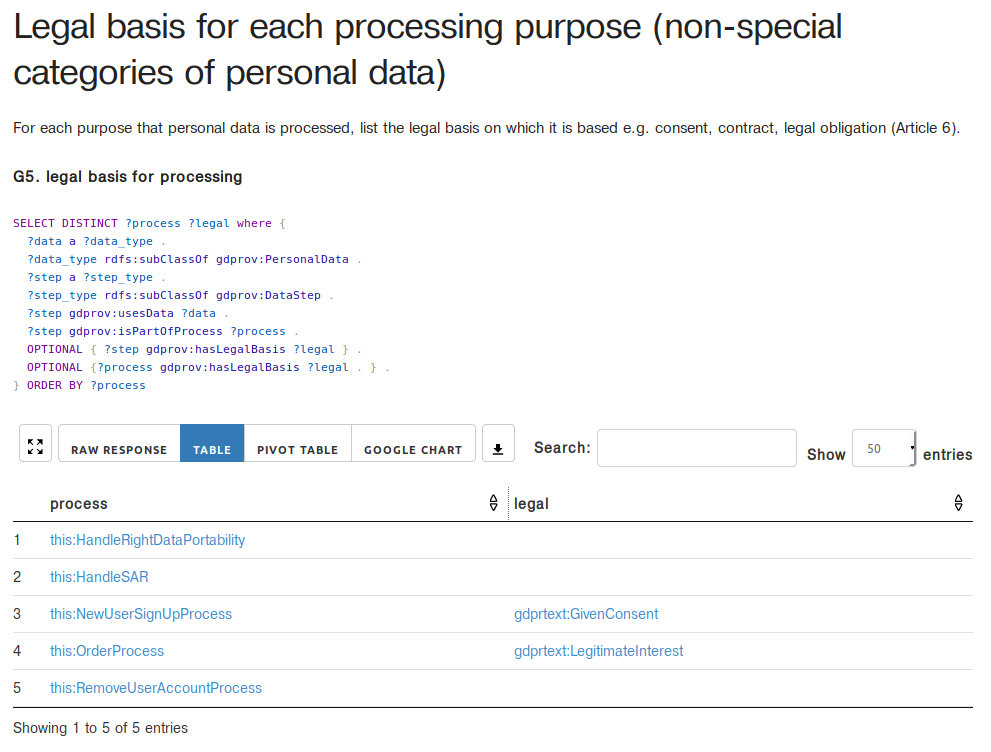
\includegraphics[width=0.75\textwidth]{img/sparql_query_demo.png}}
\caption{Retrieving information using SPARQL for query G5 in GDPR readiness checklist}
\label{fig:sparql:demo}
\end{figure}

\subsection{Evaluation}\label{sec:testing:sparql:evaluation}
The aim of this work was to represent compliance questions using SPARQL in order to retrieve information represented in RDF regarding the processing of personal data.
The demonstration using a synthetic use-case provided the basis for exploring the application of created SPARQL queries by using GDPRov and GDPRtEXT were utilised as the ontological representations of data.
The evaluation of this work, while not being exhaustive, concerns the creation of SPARQL queries and their application over a given use-case.

In terms of coverage of compliance questions represented as SPARQL queries, the exercise could not represent all of the questions within the GDPR readiness guide.
Where the reason was GDPRov not providing a required concept, the concept was identified and added in a later iteration of the ontology. 
Other reasons include a the lack of knowledge regarding representation of ambiguous information such as `indefinite' storage periods and their legal validity, and the query being out of scope for the research question of this thesis - namely activities associated with personal data and consent.
\autoref{table:sparql:dpc-2} presents an indication of these through the \textit{SPARQL} and \textit{GDPRov} columns.

Since the goal of the exercise demonstrating a compliance question could be expressed in SPARQL, the evaluation consisted of determining the extent to which this was possible. 
The expression of compliance questions using SPARQL is not novel in itself, as approaches in the SotA present their use of SPARQL in querying information related to GDPR compliance - such as in the SPECIAL, MIREL, and DAPRECO projects.
Details of their creation and implementation are sparse as pointed out in the SotA analysis in \autoref{sec:sota:analysis}, which makes it difficult to compare the SPARQL queries presented here in context of the SotA.

Of the total 63 questions within the GDPR readiness guide, 32 questions have corresponding SPARQL queries created and used in the demo.
Of the 31 questions that were not implemented, 20 questions were considered out of scope as they do not relate to the research question, with the other 3 questions lacking corresponding concepts in GDPRov to create SPARQL queries.
Of these, question \texttt{G8} concerning retention periods for personal data can be expressed using the Time ontology \cite{cox_time_2017}.
The other two, \texttt{S5} and \texttt{S7} require specification of information associated with information management and governance procedures utilised within an organisation. While these are technically not outside the scope of GDPRov, they require a larger understanding of how such processes are specified and managed, and commonly involve use of specifications to denote practices, for example ISO/IEC 27001 describing a framework for information management and protection.
Some questions not considered within scope concern information not associated with processing of personal data or consent, but which can be represented as activities using GDPRov. These include questions \texttt{C1} concerning agreements between entities or question \texttt{C4} concerning escalation procedures involving DPO.

% ---------------------------------------------------------------------------------

\section{Validating Information for GDPR Compliance using SHACL}\label{sec:testing:shacl}
This section presents the application of SHACL to validate information based on requirements of GDPR compliance.
SHACL is utilised as a validation mechanism to create a test-driven approach where information regarding processing activities is represented using semantic representations, and is first checked for correctness and then for compliance.
In this, the constraints presented in \autoref{sec:info:constraints} are utilised to determine the correctness and compliance of information, and questions presented in \autoref{sec:info:compliance-questions} are used to retrieve information for compliance.
Both the constraints and the queries are linked to the GDPR using GDPRtEXT.

The results of SHACL validations are persisted to create a `compliance graph' which enables querying for information regarding compliance, and provides more efficient testing based on reuse of ex-ante tests in ex-post testing.
The approach is demonstrated using a proof-of-concept implementation based on the evaluation of consent information on a real-world website and using GDPRov, GConsent, and GDPRtEXT to represent the information.
This approach and the implementation have been published in peer-reviewed publications concerning the conceptual model \cite{pandit_exploring_2018}, construction of a knowledge graph from information about GDPR compliance \cite{pandit_towards_2018}, and implementation testing compliance of given consent on a real-world website \cite{pandit_test-driven_2019}.
All resources regarding this work have been published online\footnote{\url{https://w3id.org/GDPRep/semantic-tests}} under an open and permissive license (CC-by-4.0).

The work presented in this section fulfils the research objectives $RO5$ and demonstrates the following:
\begin{enumerate}
    \item Utilise SHACL to validate information for GDPR compliance.
    \item Express compliance as a test-driven exercise similar to the concept of unit-testing in software engineering.
    \item Utilise results of testing ex-ante information for testing of ex-post information in order to reduce the number of tests required.
    \item Construct a compliance graph storing test results based on the concept of knowledge-graph.
    \item Demonstrate the use of compliance graph in retrieving and documenting information regarding GDPR compliance.
\end{enumerate}

A description of the approach is provided in \autoref{sec:testing:shacl:approach} which presents the role of SHACL as a validation mechanism and the creation of a compliance graph containing information relevant for compliance. The creation of SHACL constraints to represent the natural language constraints in \autoref{sec:info:constraints} is presented in \autoref{sec:testing:shacl:constraints}, with the argument for utilisation of ex-ante validations for evaluation of ex-post information presented in \autoref{sec:testing:shacl:combine}.
A proof-of-concept implementation demonstrating application of the approach is presented in \autoref{sec:testing:shacl:demo}, with the creation of documentation and compliance reports presented in \autoref{sec:testing:shacl:reports}.

\subsection{Validation Model}\label{sec:testing:shacl:approach}
\autoref{fig:shacl:model} presents a visual overview of the approach for the validation model.
The terminology consists of terms utilised by SHACL, with \textit{data graph} indicating the RDF data which is to be evaluated using SHACL, \textit{compliance graph} indicating RDF data containing information relevant for compliance, \textit{completeness} indicating the sufficiency of information i.e. all required data is present, \textit{validation} is the process of evaluating constraints on the data graph, and where \textit{testing} and \textit{evaluating} are used interchangeably with validation as synonyms to refer to the same process.
\begin{figure}[htbp]
    \centering
    \fbox{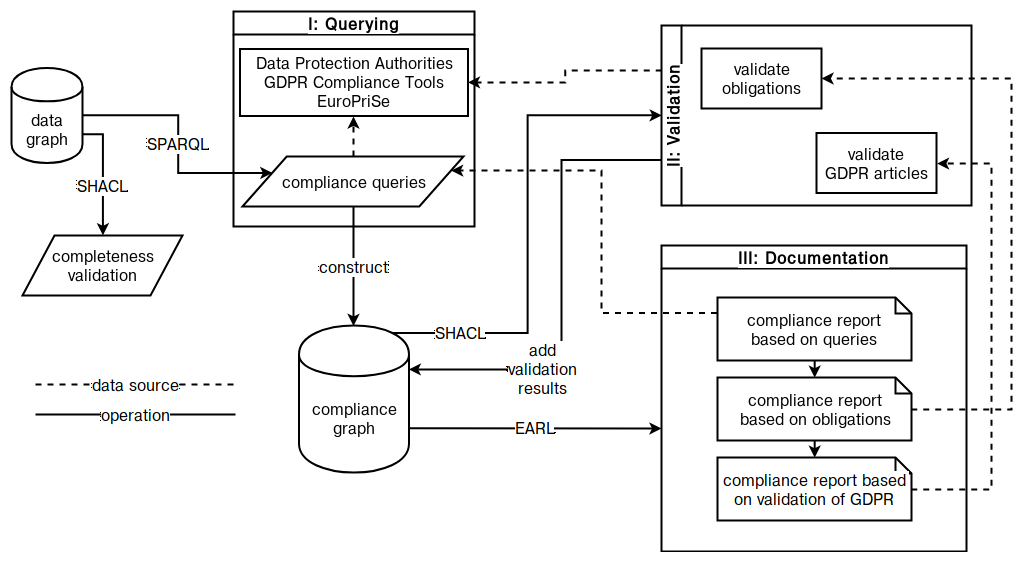
\includegraphics[width=\textwidth]{img/SHACL-model.png}}
    \caption{Overview of approach utilising SHACL to validate information for GDPR compliance}
    \label{fig:shacl:model}
\end{figure}

The approach described in the figure consists of three steps - (i) Querying, (ii) Validation, and (iii) Documentation. A data graph acts as the input and provides information about activities associated with processing of personal data and consent represented in RDF. The data graph needs to be first ensured for `completeness' - i.e. ensuring required information is present before it can be utilised for GDPR compliance.
After this, the first step of querying retrieves information for answering compliance queries by using SPARQL. This information is then added to a `compliance graph' which is separate from the data graph and stores information for determining compliance.

In the second step of validation, SHACL constraints representing obligations and requirements of the GDPR are executed over the compliance graph with the results added back to the compliance graph.
The SHACL constraints and the evaluated results are linked to specific GDPR obligations and articles.
At this point, the compliance graph contains information necessary to answer the compliance questions along with its evaluation using SHACL linked to GDPR.

In the third and final step, the information within the compliance graph is used for documentation of compliance information based on compliance questions, fulfilment of obligations, or coverage of GDPR articles. It queries the compliance graph using SPARQL by and retrieves information linked to GDPR.
The results of these can then be persisted or demonstrated using any presentation medium - such as a webpage, dashboard, or even a data file.

The use of RDF makes SPARQL and SHACL the default choices for querying and validation respectively given their status as standards.
However, the model presents a modular approach for querying, validating, and documenting information relevant to compliance. This is to enable the use of alternative technologies for carrying out the tasks associated in a particular step. 
For example, ShEx - another validation standard - can be used in lieu of SHACL to express constraints over RDF data.

The steps only represent a separation of concerns in the description of the model.
In practical uses, such as one presented in this thesis, the first and second steps are combined to consolidate the validations associated with correctness and GDPR obligations.
This is based on the assumption that missing information (which is checked by completeness validations) is a failing condition for the evaluation of compliance.
The constraints presented in \autoref{sec:info:constraints} thus incorporate expression of validations for both completeness and obligations.

\subsection{Creation of SHACL constraints}\label{sec:testing:shacl:constraints}
\subsubsection{Ontologies for expressing SHACL constraints}
\autoref{sec:testing:sparql} mentioned the dependency of SPARQL queries on the underlying data model which necessitated utilisation of the same ontological representations as those used in the information to be queried.
The same argument applies for the validation of information using SHACL, where the constraints must utilise the same ontologies as those used in the RDF it aims to validate.
An alternative is using mapping tables to convert the ontologies used in the data to a common ontology used in the validation constraints - however, this will be a difficult, if not impossible, exercise due to the complexities of finding a common model in all the ontologies that can be potentially used to represent information, such as those within the state of the art.

The constraints presented here use the developed ontologies from \autoref{chapter:vocabularies}, namely GDPRov to represent activities associated with processing of personal data and consent, GConsent to represent information about consent relevant for compliance, and GDPRtEXT to link information with the concepts and clauses of GDPR.
In this, the use of GDPRov and GConsent is complimentary in some of the constraints given their overlap in representing concepts associated with consent.
GDPRtEXT is used to link the constraint to a particular clause within the GDPR to indicate its relevancy regarding compliance. It is also used to link the validation results with clauses in the GDPR to enable querying the results based on GDPR articles, as shown later in \autoref{sec:testing:shacl:reports}.

\subsubsection{Extending SHACL concepts to associate information with GDPR}
In the assessment of information for GDPR compliance, some constraints cannot be evaluated automatically based on their qualitative requirements. For example, constraints associated with given consent that aim to evaluate whether it was `freely given' or `unambiguous'. These constraints need to be manually evaluated and their results require to be stored within the compliance graph.
To distinguish such constraints, the the SHACL concept of \texttt{NodeShape} was extended with a sub-class as \texttt{Constraint} with further sub-classes of \texttt{ManuallyCheckedConstraint} and \texttt{AutomaticallyCheckedConstraint} representing constraints that should be checked manually and automatically respectively. This is presented in Listing.\autoref{code:shacl:manual-constraint}.
The property \texttt{linkToGDPR} was created to link information with the clauses of the GDPR with the range \texttt{eli:LegalResourceSubdivision} to enable associating it with any granular part of the GDPR - such as a chapter, article, paragraph, or sub-paragraph - as GDPRtEXT uses this concept as the parent class of its concepts representing structure of GDPR.
\begin{listing}[htbp]
\begin{minted}{turtle}
:Constraint rdfs:subClassOf sh:NodeShape ;
    rdfs:label "Constraint" .
:AutomaticallyCheckedConstraint rdfs:subClassOf :Constraint, sh:NodeShape ;
    rdfs:label "Automatically Checked Constraint" .
:ManuallyCheckedConstraint rdfs:subClassOf :Constraint, sh:NodeShape ;
    rdfs:label "Manually Checked Constraint" .
    
:linkToGDPR a rdfs:Property ;
    rdfs:range eli:LegalResourceSubdivision ;
    rdfs:label "linkToGDPR" .
\end{minted}
\caption{Extending SHACL \texttt{NodeShape} to express manual and automated checking of constraints}
\label{code:shacl:manual-constraint}
\end{listing}

The constraints utilise both GDPRov and GConsent where appropriate and possible so as to verify using both ontologies. For example, Listing.\autoref{code:shacl:gdprov-gconsent} presents a constraint for checking whether each instance of consent is associated with one and only one Data Subject. In it, the concept of Data Subject could be used from GDPRov or GConsent since they both feature it. Therefore, \texttt{sh:or} in SHACL enables representing the condition where either of those could be used to express a Data Subject.
The constraint is linked to the Article 4-11 of GDPR using the property \texttt{linkToGDPR} mentioned above, and provides a human readable message when the constraint fails using the SHACL property \texttt{sh:message}.
\begin{listing}[htbp]
\begin{minted}{turtle}
:ConsentHasDataSubject a sh:PropertyShape, :AutomaticallyCheckedConstraint ;
    sh:name "Consent --> Data Subject" ;
    :linkToGDPR gdpr:article4-11 ;
    sh:path gc:isConsentForDataSubject ;
    sh:minCount 1;
    sh:maxCount 1;
    sh:or ( [ sh:class gc:DataSubject ] [ sh:class gdprov:DataSubject ] ) ;
    sh:message "Consent should be linked to Data Subject" .
\end{minted}
\caption{SHACL constraint checking Data Subject associated with consent}
\label{code:shacl:gdprov-gconsent}
\end{listing}

\subsubsection{Using SHACL-SPARQL}

SHACL-SPARQL\footnote{\url{https://www.w3.org/TR/shacl/\#shacl-sparql}} is an extension of SHACL core features and provides the use of SPARQL queries to retrieve information failing the associated constraint. Listing.\autoref{code:shacl:SHACL-SPARQL} presents alternative representations of the same constraint in SHACL core and SHACL-SPARQL.
The constraint aims to ensure all consent instances have a timestamp.
The SHACL-SPARQL constraint features a SPARQL query that filters instances that have a specified timestamp based on properties provided by GConsent, GDPRov, or PROV-O, while the SHACL core representation uses a \texttt{PropertyShape} to assess the same.
\begin{listing}[htbp]
\begin{minted}{sparql}
# SHACL-SPARQL
sh:select "
    SELECT $this WHERE {
        FILTER NOT EXISTS { $this gc:atTime ?time } .
        FILTER NOT EXISTS { $this prov:generatedAtTime ?time } .
        FILTER NOT EXISTS { $this a gdprov:ConsentAgreementTemplate } .
    } " .
\end{minted}
\begin{minted}{turtle}
# SHACL Core
_:ConsentHasTimestamp a sh:PropertyShape ;
    sh:or (
        [ sh:path gc:AtTime . sh:minCount 1; ] ;
        [ sh:path prov:generatedAtTime . sh:minCount 1; ] ;
        [ sh:path gdprov:ConsentAgreementTemplate . sh:minCount 1; ] ;
    ) .
\end{minted}
\caption{Expressing the same constraint in SHACL-SPARQL and in SHACL core}
\label{code:shacl:SHACL-SPARQL}
\end{listing}

The advantages of using SPARQL queries in SHACL constraints is access to information in instances that fail the validation. This is useful in inserting information about the instance in the test reports, such as the ID or IRI, or even the specific triple that needs correction or verification.
The use of SHACL-SPARQL also allows use of the SPARQL queries from \autoref{sec:testing:sparql} by modifying them to retrieve information that will fail the constraint.

\subsubsection{Validating manually evaluated constraints}
For the manually evaluated constraints represented using \texttt{ManuallyCheckedConstaint}, the result arising from its assessment indicates whether the constraint fails or passes, and is therefore a boolean value.
Therefore, the assessment of manually checked constraints is based on verifying a boolean value associated with the constraint through the SHACL property \texttt{sh:hasValue} which indicates the expected value of a property.
An example of this is presented in Listing.\autoref{code:shacl:boolean} which represents a constraint checking whether the given consent was freely given.
The assessment is based on explicitly inserting a triple within the data graph that denotes the manually inspected condition of freely given through the property \texttt{m:consentIsFreelyGiven} whose value must be true to indicate compliance.
The messages of a manually checked constraint are prefixed with \textit{(MANUAL-TEST)} to indicate their qualitative nature in human-intended messages.
\begin{listing}[htbp]
\begin{minted}{turtle}
:ValidconsentIsFreelyGiven a sh:PropertyShape, :ManuallyCheckedConstraint ;
    :linkToGDPR gdpr:article4-11 ;
    sh:name "Consent == Freely Given" ;
    sh:path m:consentIsFreelyGiven ;
    sh:hasValue true ;
    sh:message "(MANUAL-TEST) Consent should be freely given" .
\end{minted}
\caption{Evaluating manually checked constraints using boolean values}
\label{code:shacl:boolean}
\end{listing}

\subsection{Utilising ex-ante test results for ex-post validations}\label{sec:testing:shacl:combine}
Based on distinguishing information about activities in ex-ante and ex-post phases, the constraints will also need to be expressed to evaluate these phases separately.
This will cause duplication of evaluations based on testing of same information across both phases. 
For example, in evaluating whether given compliance is compliant with the requirements of GDPR compliance - which is an ex-post evaluation of compliance - information about criteria such as whether the consent was informed are based on the artefacts shown during the request for consent. The information shown when consent was requested is (usually) part of ex-ante activities and (usually) is common to a large number of consent requests - such as the online consent request form shown to all users on a website. Therefore, the assessment of whether it fulfils the obligations associated with informed consent is also common to all instances of consent based on it. 
By performing an evaluation of this artefact in the ex-ante phase, its (successful) results can be reused for evaluation of all consent based on it in the ex-post phase.
This represents utilisation of ex-ante test results in ex-post validation of a constraint.

The abstraction of this can be summarised based on considering the ex-ante information as that associated with the model or plan of activities, and the ex-post information to be regarding the execution of those activities. Since the model is a common template for all execution of the activities, some of the common ex-ante validations can be performed prior to the execution and the results persisted for use in ex-post validations.
This information, which are expressed as SHACL validation reports for the purposes of this thesis, are persisted in the compliance graph in ex-ante phase validations, and are used as part of the data graph in the ex-post validations.

An example of an ex-post validation incorporating ex-ante test results is presented in Listing.\autoref{code:shacl:model-constraint}.
The constraint is automatically evaluates the outcome of a previous SHACL validation concerning the given consent model in ex-ante phase indicated by \texttt{sh:ValidationReport} with the property \texttt{sh:conforms} used by SHACL to indicate whether an evaluated data graph has passed or failed the given constraints.
\begin{listing}[htbp]
\begin{minted}{turtle}
:ConsentModelConstraints a sh:NodeShape ;
    sh:targetClass sh:ValidationReport ; 
    sh:property :ValidationReportConforms ;
    rdfs:label "Given Consent following Consent Model constraints" .

:ValidationReportConforms a sh:PropertyShape, :AutomaticallyCheckedConstraint ;
    sh:path sh:conforms ;
    sh:hasValue true ; 
    sh:message "Consent Model should be compliant for given consent to be valid" ; 
    sh:name "Check validation report says data conforms" .
\end{minted}
\caption{Utilising ex-ante test results for consent model in evaluating ex-post instances of given consent}
\label{code:shacl:model-constraint}
\end{listing}

\subsection{Proof-of-concept implementation}\label{sec:testing:shacl:demo}
For a proof-of-concept implementation of the approach, the consent dialogue on the Quantcast\footnote{Web archive snapshot \url{https://web.archive.org/web/20190430014325/https://www.quantcast.com/}} was utilised as an use-case and evaluated for GDPR compliance.
Information from the consent dialogue was manually analysed and represented using GDPRov and GConsent to create the data graph. Additionally, information from other pages on the website were also analysed to identify more information about the purposes, processing, personal data, and third parties mentioned in the consent dialogue.
Resources associated with the implementation are available in a public repository\footnote{\url{https://github.com/coolharsh55/GDPR-semantics-demo/}}.

The choice of use-case was made based on Quantcast being a provider of GDPR consent collection mechanism using the IAB consent framework\footnote{\url{https://advertisingconsent.eu/}} - which is the largest consent framework in use and is based on the collection of consent and sharing of personal information using the internet. The Quantcast website was also one of the few (at the time and to the authors’ knowledge) that allowed changing/withdrawing consent using the same dialogue as the one used to request/provide it.

The aim of this exercise is to demonstrate the use of SHACL in validating information for compliance, and the use of ex-ante test results in validating information in ex-post phase.
It is not intended to act as a compliance evaluation\footnote{The Data Protection Commission of Ireland opened an enquiry on 02-May-2019 into the practices of Quantcast in relation to ``processing and aggregating of personal data for the purposes of profiling and utilising the profiles generated for targeted advertising is in compliance with the relevant provisions of the GDPR'' - source: \url{https://www.dataprotection.ie/en/news-media/press-releases/data-protection-commission-opens-statutory-inquiry-quantcast}. The enquiry was announced well after the completion of the presented work, but bears relevance in terms of its findings - which have not been announced as of yet.} of Quantcast, but serve as a demonstration of the usefulness of technological measures, and particularly the semantic web, in representing, querying, and documenting information for compliance.

\subsubsection{Description of Consent Dialogue}
The consent dialogue, depicted in \autoref{fig:shacl:quantcast-consent-dialogue}, is presented to the user upon visit to the Quantcast website. The consent dialogue consists of multiple pages or panels presenting various abstractions of information and choices which the user can interact with.
The first panel, depicted in the figure as \texttt{(a)}, presents a brief description of processing and purposes and provides an option to provide consent\footnote{Note for clarification: Clicking the `I Accept' button signals consent for all specified purposes, as can be verified by clicking on the `Change Consent' button at the bottom of the page to show the selected choices in the consent dialogue. We avoided the interpretation of qualitative assessments in evaluating whether the "I Accept" button fails consent requirements such as not having options pre-ticked or pre-chosen by default, though we believe this does not satisfy the requirements of valid consent under GDPR. We instead represent these qualitative constraints as \texttt{ManuallyCheckedConstraint} and assume their assessment to always be true.} using the `I Accept' button. Further information is made available through the `Show Purposes' button. Upon giving consent at any stage of the dialogue, clicking the `Change Consent' link in the footer at the bottom of the page shows the consent dialogue with the selected consent choices.
\begin{figure}[htbp]
    \begin{minipage}[b]{0.5\linewidth}
        \centering
        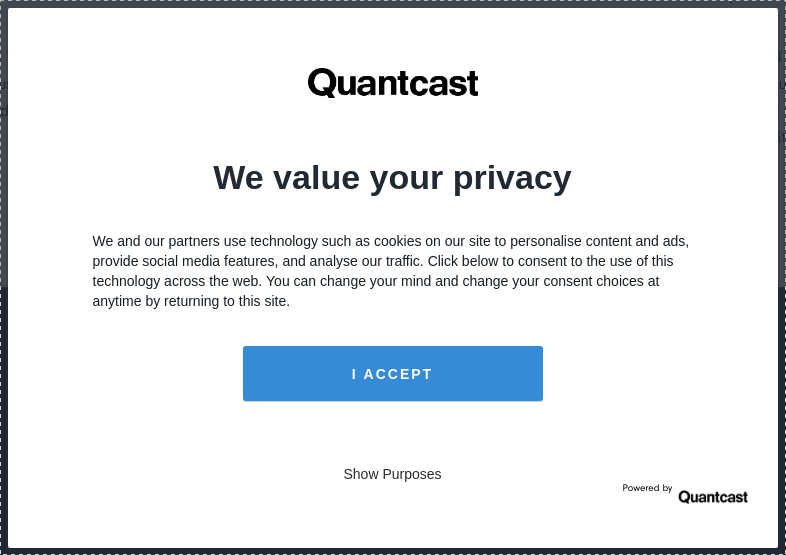
\includegraphics[width=\linewidth]{img/quantcast_consent_screen.png}
        \vspace{0.35cm}
    \end{minipage}
    \begin{minipage}[b]{0.5\linewidth}
        \centering
        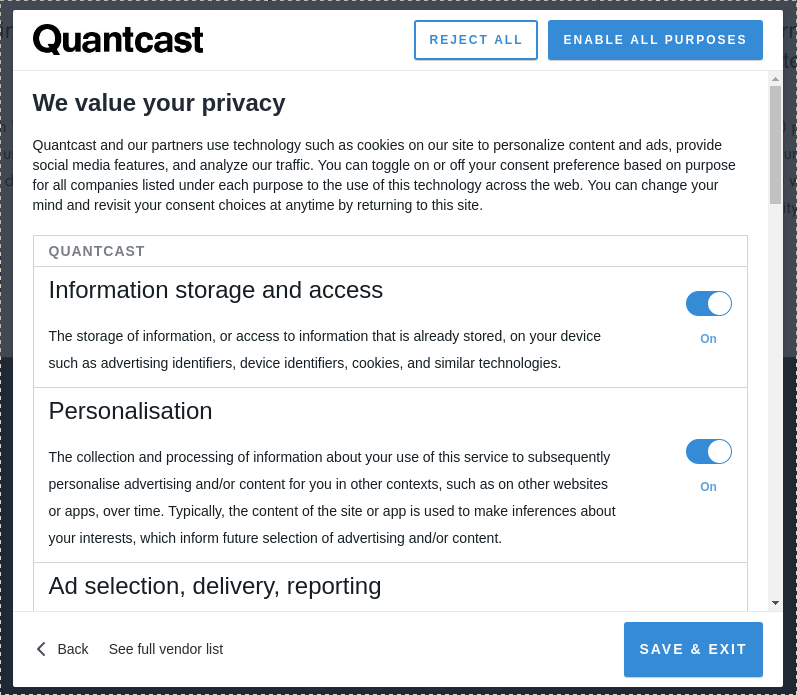
\includegraphics[width=\linewidth]{img/quantcast_consent_I_agree.png}
    \end{minipage}
    \begin{minipage}[b]{0.5\linewidth}
        \centering
        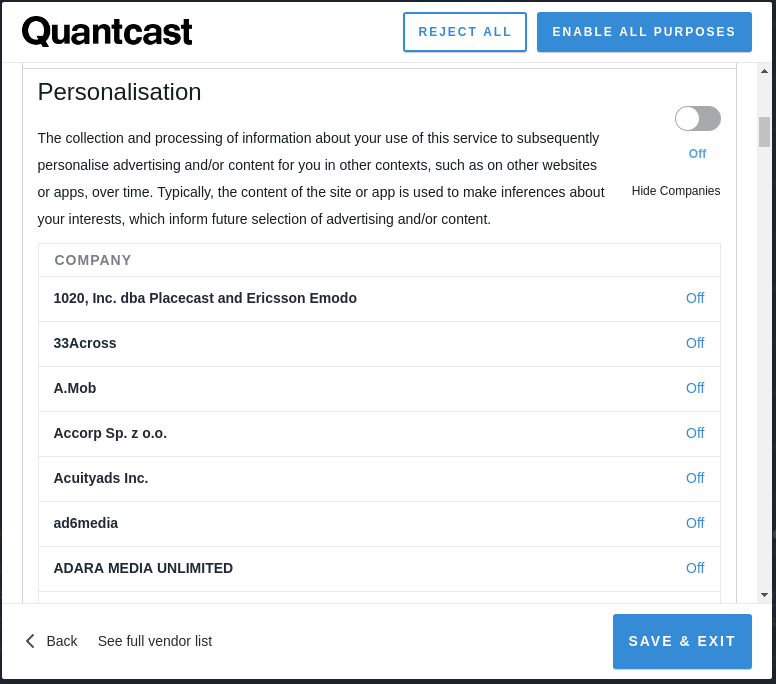
\includegraphics[width=\linewidth]{img/quantcast_third_parties.png}
    \end{minipage}
    \begin{minipage}[b]{0.5\linewidth}
        \centering
        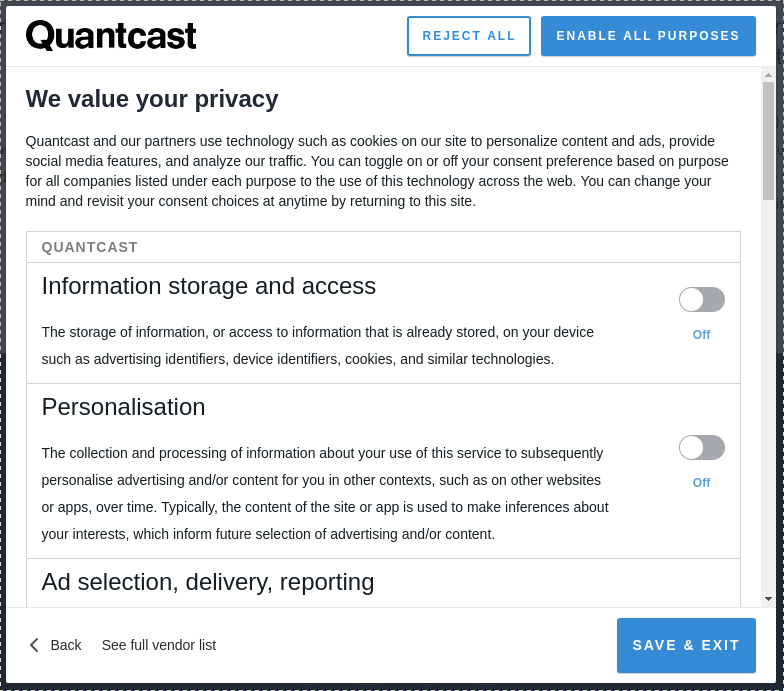
\includegraphics[width=\linewidth]{img/quantcast_consent_info.png}
    \end{minipage}
    \caption{Consent dialogues on \url{quantcast.com} (clockwise from top-left) (a) first screen (b) default options on selecting “I Accept” (c) default options on selecting “Show Purposes” (d) Third parties listed for purpose “Personalisation”}
    \label{fig:shacl:quantcast-consent-dialogue}
\end{figure}

\subsubsection{Extracting Purposes, Processing, and Personal Data from Consent Dialogue}
Clicking the `Show Purposes' dialogue opens the second panel containing information about the  purposes and third parties associated with consent, displayed in figure as \texttt{(b-d)}.
The first section provides information about processing of personal data carried out by Quantcast. Its structuring of information consists of the title specifying the purpose of processing, for example - ``\textit{Information storage}'', followed by a textual description of the persona data categories involved and the processing operations to be performed on them.

The purpose was represented using GDPRov and GConsent as instances of \texttt{gdprov:Process} and \texttt{gc:Purpose} with the title from consent dialogue specified as its label using \texttt{rdfs:label}. 
Information about processing and personal data categories was manually extracted from the text and represented as - \texttt{gdprov:Step} and \texttt{gc:Processing} for processing, and \texttt{gdprov:PersonalData} and \texttt{gc:PersonalData} for personal data.

The consent dialogue was represented using GDPRov as \texttt{ConsentAgreementTemplate} to indicate an ex-ante artefact provided when requesting consent.
Since the consent dialogue offers granular choices from which the user can choose any option individually, the question of its semantic representation leads to two solutions - first where the entire consent dialogue and all consent choices are considered a single instance of consent, and second where each individual and independent choice is considered an instance of consent.
Since given consent for an individual option in the dialogue could be revoked without affecting other choices, each independent option was chosen to be modelled as an instance of consent.
As the consent dialogue acts as a common template for all options, its representation as a `bundle' of consent templates was added to an updated version of GDPRov as \texttt{gdprov:ConsentAgreementTemplateBundle}. This enabled representing a common artefact used to request separate instances of consent.
Listing \autoref{code:shacl:consent-dialogue} provides an example representation of the information from the consent dialogue using this data model.
\begin{listing}[htbp]
\begin{minted}{turtle}
:ConsentRequestDialog a gdprov:ConsentAgreementTemplateBundle ;
    rdfs:label "Consent Dialog shown to the user" ;
    rdfs:comment "Dialog that shows - We value your privacy...
        ... customise their choice by clicking on 'Show Purposes'." ;
    gdprov:usesConsentAgreementTemplate 
        :CATQInfoStorageAccess, :CATQPersonalise, :CATQAds, 
        :CATQMeasure, :CATTPInfoStorageAccess, :CATTPPersonalise, 
        :CATTPAds, :CATTPContentSelection, :CATTPMeasure, :CATTPGoogle .

:CATQInfoStorageAccess a gdprov:ConsentAgreementTemplate, gc:Consent ;
    rdfs:label "consent for CATQInfoStorageAccess" ;
    gc:forPurpose :InformationStorageAccess ;
    gc:forProcessing :StoreIdentifiers, :UseIdentifiers ;
    gc:forPersonalData :Cookie, :AdIdentifier, :DeviceIdentifier ;
    gc:hasLocation <https://quantcast.com/> ;
    gc:withdrawBy <https://www.quantcast.com/#displayConsentUI> ;
    gc:inMedium "dialog box on website" ;
    gc:hasStatus gc:ConsentStatusRequested .
\end{minted}
\caption{Representation of consent dialogue as a bundle of consent requests}
\label{code:shacl:consent-dialogue}
\end{listing}

\subsubsection{Extracting Third-Parties from Consent Dialogue}
In the bottom half of the second panel, the consent dialogue provides information about purposes of sharing data with third parties and a list of recipients for each purpose. This can be seen in the figure in panel \texttt{(c)}.
Consent for each purpose for sharing data with third parties can be individually acted upon by means of a radio button or toggle. Opting to provide consent for a purpose is taken as providing consent for all listed third parties for that purpose, i.e. there is no granular control for consent for individual third parties. 

The third parties were defined using \texttt{gdprov:ThirdParty} and \texttt{gc:ThirdParty}.
Although the names of purposes are the same in sections describing processing by Quantcast (top-half) and by third parties (bottom-half), these were declared as separate instances to reflect separation of choices to provide consent.
Third parties were associated with a particular process by first creating an instance of a data sharing step using \texttt{gdprov:DataSharingStep} and \texttt{gc:DataStep}, and then linking the third party using the property \texttt{gc:SharesDataWithThirdParty}.

\subsubsection{Gathering additional information from Quantcast website}
The consent dialogue does not provide information on how the personal data categories are collected, or the data sources for personal data. To investigate this, an analysis of information about products and services provided Quantcast on their website along with their policies was carried out to identify relevant information which could be added to complete the use-case.

\textit{Measure} is a free service offered by Quantcast that provides analytics regarding audience (visitors) to websites. It uses the following categories of personal data: \textit{Demographics} (age, gender, family, location, income, education, and occupation), \textit{Psychographics} (purchase history, brand preference, cars driven, media consumption), \textit{Engagement} (categorise visitors as passers-by, regulars, and fanatics), and \textit{Traffic} (platform - web and mobile web, country, time period). Of these, data categories of Demographics and Psychographics were included in the data graph as being relevant to the information provided in the consent dialogue. Their source was not indicated by Quantcast and therefore was not added to the data graph.
For Psychographics, Quantcast specifies that it uses information from third-parties (Experian, Mastercard, DLX, TiVo, and Netwise) to `augment' its profiles. The third parties were defined as the the source for this data based on this information.
The profiles mentioned above are described on the webpage as broad categories of data in the form of Shopping Interests, Media Interests, Business \& Occupation, Geography, and Political Interests. These were added to the data graph as personal data categories.

\textit{Targeting} is a service which provides selecting audiences/users based on personal data attributes (similar to those in Measure). While Quantcast\footnote{The service provided by Quantcast is in essence similar to that provided by Facebook - it acts as the mediator between providers and consumers by matching the criteria to user profiles. For example, it mentions an example where the target audience is ``women 18-34 who love shopping, travelling and wine'', which implies that it must know about a) gender b) age range c) website history d) purchase history e) travel history, It further elaborates, ``We build a custom model based on millions of available data points about your audience, such as their pre-search behaviours, demographics, and past purchases.''} does not explicitly say that it uses the same personal data collected and used in Measure, this implication was implicit in its description. However, since this is an assumption, it was not included in the data graph.

\textit{Measurement} is a service similar to Measure and Targeting in its use of audience profile, with the key difference between provision of service beyond website audiences, such as for campaigns. It describes data categories such as Website Traffic, Demographics, Interests, Search behaviours, and Media consumption, which were added to the data graph.

The privacy policy provided by Quantcast provides information regarding personal data categories as Cookies, Tags, and Log data - which were added to the data graph. 
The use and collection of emails used to contact Quantcast were also incorporated.
Data retention periods are provided as ``for as long as necessary'', with an explicit limit for log data provided as 13 months. Due to the ambiguity and pending legal resolution of temporal limits, this information was not added to the data graph.
The privacy policy also described GDPR rights regarding right to access, right to rectify, right to restrict processing, right to deletion, right to data portability, and provided a link\footnote{NOTE: The rights information page could not be accessed in this case with the webpage providing an error regarding Quantcast cookies not being set."} for contact and more information. This link was used as the IRI for activities associated with these rights.

\subsubsection{Validating using SHACL}
As the use-case concerns consent, the constraints associated with consent in \autoref{sec:info:constraints} were used to validate the information using the approach described in \autoref{sec:testing:shacl:approach}.
For evaluation, three sets of constraints were developed to validate: (a) only the ex-ante model of consent dialogue, (b) instances of given consent, and (c) reusing results of ex-ante consent dialogue tests to validate given consent.
This allowed an analysis and comparison of combining ex-ante and ex-post validations, and to demonstrate the benefits in terms of reduced validations and reuse of compliance information.

SHACL constraints were executed using the TopBraid SHACL binary\footnote{\url{https://github.com/TopQuadrant/shacl}}.
A bash\footnote{\url{https://www.gnu.org/software/bash/}} script enabled automation in execution of constraints as different approaches (ex-ante, ex-post, combination of both) and persistence of test results as separate files.

For ease of evaluation, a combined data graph was created consisting of data from Quantcast and the ontologies used - GDPRov, GConsent, GDPRtEXT. 
The data graph and test results were enhanced using a semantic reasoner\footnote{HermiT \url{http://www.hermit-reasoner.com/}} to identify and add additional triples derived from inferences.
The resulting data was added to a triple store\footnote{GraphDB Free Edition \url{http://graphdb.ontotext.com/}} in separate graphs representing the data graph and compliance graph respectively.

\subsection{Generating reports using SPARQL}\label{sec:testing:shacl:reports}
The triple store enabled querying of information to generate compliance reports and documentation.
The use of GraphDB provided access to some in-built reasoning capabilities\footnote{\url{http://graphdb.ontotext.com/free/devhub/inference.html}} which were useful in the querying process.
While a number of SPARQL queries were constructed based on the compliance questions and are available for introspection in the code repository, only one is provided here as an example to demonstrate retrieval of information and documentation of compliance information.

The SPARQL query, listed in Listing \autoref{code:shacl:sparql-report}, retrieves information about each tested validation constraint, its result, link to GDPR, and whether it passed or failed.
The results, shown in \autoref{table:shacl:sparql-report} act as a test report, and contain the constraint description (Name), type - automatic (A) or manual (M), link to GDPR, result - pass (P) or fail (F), and node (instance in data graph) if it failed a constraint.
The report also contains a failure message associated with the constraint that is not shown in table due to space limitations.
\begin{listing}[htbp]
\begin{minted}{sparql}
PREFIX c: <http://example.com/Quantcast/shapes#>
PREFIX sh: <http://www.w3.org/ns/shacl#>
SELECT DISTINCT ?name ?test ?gdpr ?result ?node ?msg
WHERE {
    ?x a c:Constraint .
    ?x sh:name ?name .
    BIND(
        IF(EXISTS{?x a c:AutomaticallyCheckedConstraint},
            "Automatic"^^xsd:string, "Manual"^^xsd:string)
        as ?test)
    OPTIONAL { ?x c:linkToGDPR ?gdpr }
    BIND(
        IF(EXISTS{?y sh:sourceConstraint ?x},
            "FAIL"^^xsd:string, "PASS"^^xsd:string)
        as ?result)
    OPTIONAL {
        FILTER EXISTS { ?y sh:sourceConstraint ?x } .
        ?y sh:focusNode ?node .
    	?y sh:resultMessage ?msg . }
} ORDER BY ?name
\end{minted}
\caption{SPARQL query for report listing validation results linked with GDPR}
\label{code:shacl:sparql-report}
\end{listing}

\definecolor{lightred}{RGB}{255,225,225}

\begin{center}
    \footnotesize
\begin{tabularx}{\linewidth}{|l|X|X|X|l|}
\caption{SHACL validation report linked to GDPR} \label{table:shacl:sparql-report} \\
\toprule
\textbf{Name} & \textbf{Type} & \textbf{GDPR} & \textbf{Result} & \textbf{Node} \\ 
\midrule
\endfirsthead

\caption*{SHACL validation report linked to GDPR (cont'd)} \\
\toprule
\textbf{Name} & \textbf{Type} & \textbf{GDPR} & \textbf{Result} & \textbf{Node} \\
\midrule
\endhead


\midrule
\multicolumn{5}{r@{}}{\footnotesize (Cont'd on following page)}\\
\endfoot

\endlastfoot
    
Consent $\neq$ Inactivity & M & R32 & P &  \\ \hline
Consent $\neq$ Pre-ticked Boxes & M & R32 & P &  \\ \hline
Consent $\neq$ Silence & M & R32 & P &  \\ \hline
Consent $\rightarrow$ Data Subject & A & A4-11 & P &  \\ \hline
Consent $\rightarrow$ Given To & A &  & P &  \\ \hline
Consent $\rightarrow$ Location & A &  & P &  \\ \hline
Consent $\rightarrow$ Medium & A & A7-2 & P &  \\ \hline
Consent $\rightarrow$ Personal Data & A & A4-11,R32 & P &  \\ \hline
Consent $\rightarrow$ Processing & A & A4-11,R32 & P &  \\ \hline
Consent $\rightarrow$ Provided By & A & A7-2 & P &  \\ \hline
Consent $\rightarrow$ Purpose & A & R32,R42 & P &  \\ \hline
Consent $\rightarrow$ Status & A &  & P &  \\ \hline
\rowcolor{lightred} Consent $\rightarrow$ Timestamp & A &  & F & Q:Consent20190415120753 \\ \hline
\rowcolor{lightred} Consent $\rightarrow$ Timestamp & A &  & F & Q:Consent20190415140000 \\ \hline
Consent $\equiv$ Choice & M &  & P &  \\ \hline
Consent $\equiv$ Freely Given & M & A4-11 & P &  \\ \hline
Consent $\equiv$ Specific & M & A4-11 & P &  \\ \hline
Consent $\equiv$ Statement of Clear Action & M & A4-11 & P &  \\ \hline
Consent $\equiv$ Unambigious & M & A4-11 & P &  \\ \hline
Consent Generating Activity & A &  & P &  \\ \hline
Consent Request $\equiv$ Clear & M & R32 & P &  \\ \hline
Consent Request $\equiv$ Concise & M & R32 & P &  \\ \hline
Consent Request $\equiv$ Not Disruptive & M & R32 & P &  \\ \hline
Consent Template & A &  & P &  \\ \hline
Ease of Withdraw Consent & M & A7-3 & P &  \\ \hline
Many Processing x One Purpose & A & R32 & P &  \\ \hline
\rowcolor{lightred} One Processing x Many Purposes & A & R32 & F & Q:Consent20190415120753 \\ \hline
\rowcolor{lightred} One Processing x Many Purposes & A & R32 & F & Q:Consent20190415140000 \\ \hline
\rowcolor{lightred} Personal Data $\rightarrow$ Storage Period & A & A13-2-a & F & Q:CATQInfoStorageAccess \\ \hline
\rowcolor{lightred} Personal Data $\rightarrow$ Storage Period & A & A13-2-a & F & Q:CATTPInfoStorageAccess \\ \hline
\rowcolor{lightred} Personal Data $\rightarrow$ Storage Period & A & A13-2-a,R39 & F & Q:Consent20190415120753 \\ \hline
\rowcolor{lightred} Personal Data $\rightarrow$ Storage Period & A & A13-2-a,R39 & F & Q:Consent20190415140000 \\ \hline
Right to Withdraw & A & A7-3 & P &  \\ \hline
Separation of Processing & M & R43 & P &  \\ \hline
Third Party Categories & A & A44 & P &  \\ \hline
Third Party Identities & A & A13-1-e & P &  \\ \hline
Third Party Identities & A & A30-1-d & P &  \\ \hline
Third Party Identities & A & A44 & P &  \\ \hline
Third Party Safeguards & A &  & P &  \\ \hline
Withdraw Consent Information & M & A7-3 & P &  \\
\bottomrule
\end{tabularx}
\end{center}

The rows which correspond to failed constraints are manually highlighted to provide an indication of the use of information in a visual medium - such as a dashboard.
The query and its results can both be persisted in machine-readable serialisations using standards for representations, making them interoperable and capable of automation.
The information derived from such validations and querying is useful to generate compliance documentation and reports for an organisation to oversee their compliance with the GDPR - which is itself an obligation mandated by the GDPR.

\subsection{Evaluation}

\subsubsection*{Effectiveness of combining ex-ante and ex-post validations}
In order to understand the number of validations in the testing process, consider the set $V_{t}$ consisting of all validations that should be evaluated in order to determine the validity of given consent. This set consists of validations evaluating the information in the consent dialogue box which is common to all instances of given consent - these are represented by $V_{a}$. The remaining validations consist of evaluating information specific to that instance of given consent, such as timestamps, and are represented by $V_{p}$. 
To summarise, the set of validations consists of validations evaluating the consent dialogue and the information within the given consent, with the relation $V_{t} = V_{a} + V_{p}$.

$V_{a}$ is required to be carried out as part of ex-ante compliance evaluations where the organisation must monitor and ensure its activities are compliant before any processing takes place. In this case, the consent dialogue box is required to be evaluated and found compliant before any consent is requested. Therefore, $V_{a}$ represents ex-ante validations and $V_{p}$ represent ex-post validations.

If the results of $V_{a}$ are persisted, then they can be reused in the evaluation of given consent by simply checking whether the outcome of $V_{a}$ was valid or invalid - which is a single validation. Therefore, the total validations to be performed when combining ex-ante and ex-post validations is now $V_{t} = 1(V_{a}) + V_{p}$ - which is efficient assuming $V_{a} > 1$.

In the use-case of consent dialogue presented in this section, $V_{t}=59$ validations of which $V_{a}=57$ validations and $V_{p}=2$ validations. If all validations were evaluated for given consent, each instance of given consent would need $59$ validations. Whereas, if the ex-ante validations were reused and only the ex-post validations were evaluated, then each instance of given consent would need only $3$ validations to be evaluated ($1$ validation to evaluate $V_{a} + 2$ validations from $V_{p}$). While these numbers are use case specific, it clearly demonstrates that the approach is more efficient in terms of validations and determining validity of given consent. This is assuming the ex-ante model of consent dialogue was found compliant in the ex-ante stage, and therefore its validation only evaluated the presence of a test report affirming its compliant status.

\subsubsection*{Comparison with SotA}

Approaches in the SotA which evaluate compliance (\autoref{sota:analysis:compliance}) include the those that use the semantic web technologies to express the requirements and to evaluate their fulfilment.
The SPECIAL project uses a semantic reasoner to determine whether a given combination of processing operations expressed as OWL2 class axioms are valid \cite{westphal_spirit_2018}, while the work presented by Vos et. al \cite{vos_odrl_2019} uses ODRL profiles to express requirements which are converted to and evaluated using Answer Set Programming (ASP).
The MIREL project detects violations of the GDPR by utilising the PrOnto ontology \cite{palmirani_pronto_2018,palmirani_pronto_2018-1,monica_modelling_2018} to model legal concepts and LegalRuleML to model norms, which are then applied over a BPMN use-case using Regorous to generate a report \cite{monica_modelling_2018}.
The DAPRECO project uses PrOnto along with Reified Input/Output logic (RIO) \cite{robaldo_reified_2017} to specify norms and rules to create a knowledge base \cite{bartolini_agile_2019} which is used to compare GDPR with ISO and to determine compliance.
These efforts show the variance in evaluation of compliance and the use of semantic web technologies in evaluation of compliance.
The resources provided by Vos et. al \cite{vos_odrl_2019} and DAPRECO project \cite{bartolini_agile_2019} provide constraints expressed using logic-based formalisms and which are available as open access. 


\subsection*{Conclusion}
The work described in this section demonstrates how SHACL can be used to validate information for correctness and adherence to obligations mandated by GDPR based on the interpretation of compliance questions from \autoref{chapter:information}. In this form, SHACL can be used to evaluate compliance, though the presented work focused more on the validation of constraints based on the concept of compliance questions.
Compared to the state of the art in \autoref{chapter:sota}, the work regarding SHACL is novel in that no other approach currently specifies using it to validate information for GDPR.
The utilisation of ex-ante test results in ex-post validations is also novel within the state of the art.
In comparison with SHACL, approaches in the SotA provide a more formal approach based in logic where legal norms can be expressed in terms of requirements and evaluated to determine compliance.
In turn, SHACL provides a validation framework where the results can be persisted as a graph and queried. In addition, the SHACL validations can be linked to the GDPR, as demonstrated using GDPRtEXT, which makes it possible to use SHACL to verify the output of other compliance evaluation approaches and record the outcome as a test result linked to GDPR clauses, thereby creating a graph of compliance.
This also provides an opportunity to explore the reuse of existing approaches and resources regarding evaluation of GDPR compliance where SHACL is used to generate an interoperable overview of the evaluation results while abstracting the underlying outputs from various approaches.

\section{Conclusion}\label{sec:testing:conclusion}

\subsubsection*{Summary of work presented}
\autoref{sec:testing:sparql} presented the use of SPARQL queries for representing compliance queries and retrieving information associated with compliance that was represented using GDPRov and GDPRtEXT ontologies.
The work fulfilled the research objective $RO4$ by representing the compliance questions as SPARQL queries and demonstrating their application using a real-world use-case.
The demonstrated application used questions from GDPR readiness guide published by the Data Protection Commission of Ireland in 2017 to assist organisations in assessing their adherence to compliance requirements of the GDPR.
The created SPARQL queries retrieved information for answering these compliance questions for a synthetic use-case based on the scenario of an online shopping service.
The queries and the demo were published in a peer-reviewed publication \cite{pandit_queryable_2018} at the SEMANTiCS conference and are available online as an application with the resources provided in a code repository.

\autoref{sec:testing:shacl} presented the use of SHACL to validate information regarding its correctness and adherence to obligation towards GDPR compliance.
This work fulfilled the research objective $RO5$ by validating information using SHACL and linking the results with relevant clauses of GDPR for compliance documentation.
The SHACL validation utilised constraints developed from analysis of compliance questions as presented in \autoref{sec:info:constraints}.
An approach for the validation process using SHACL was presented in which ex-ante test results were reused in the validation of ex-post information. This enabled efficient evaluations by reducing the number of validations required in the ex-post phase, and also enabled associating the compliance of ex-ante information with that of its corresponding ex-post information.
A demonstration of the approach was provided through an use-case in which the consent dialogue on a real-world website was represented using the developed ontologies and validated using SHACL.
The results of the validation were queried using SPARQL to generate documentation for compliance in the form of a test report which showed the compliance status of different obligations and highlighted failing tests as action items for meeting compliance requirements.
The approach of using SHACL and the combination of ex-ante and ex-post validations was published in a peer-reviewed publication \cite{pandit_towards_2018} at the SEMANTiCS conference in 2018, while the demonstration was published in a peer-reviewed publication \cite{pandit_test-driven_2019} at SEMANTiCS 2019.
The resources associated with the work have been made available online in a code repository.

This chapter, through both presented works, provides an application of the developed ontologies presented in \autoref{chapter:vocabularies} for querying and validating information about GDPR compliance.
It serves to demonstrate the usefulness of these ontologies, as well as provide an indication of their role in the representation of information.
The chapter also demonstrates the use of semantic web technologies in representing, querying, and validating information for GDPR compliance.

The modular test-based approach can be used with existing representations in non-RDF data that are evaluated using other tools and methods by adding semantics to the test results and reports to link them with relevant information in GDPR. This will enable the utilisation of a validation method such as SHACL to evaluate its correctness and a querying method such as SPARQL to retrieve information in the form of compliance test reports. 

The advantages of representing processes with semantics go beyond testing for compliance as representation of processes are also useful for planning of operations and internal documentation. Semantic representations of processes can assist in automating the generation of documentation such as privacy policies where processes are listed along with their purpose, legal basis, and use of personal data. Privacy policy generators that generate boilerplate policies exist online, but do not currently incorporate semantics. The use of semantics allows queryable machine-readable metadata that can be used in tools towards understanding and evaluating policies for users and authorities.

\subsubsection*{Re-usability of developed resources}
The interpretation of compliance questions in the GDPR readiness document using SPARQL and its application in the synthetic use-case demonstrates the potential application and usefulness of SPARQL queries to retrieve information relevant for compliance.
However, it also showcases that the creation of SPARQL is highly dependant on utilising the same ontological concepts as the data it is querying. Therefore, such SPARQL queries are use-case dependant, and by definition do not have re-usability beyond the data they were created for.
The same is true for the constraints represented in SHACL, which are dependent on the underlying ontologies used to represent the data graph it intends to validate.

Using the analysis and natural language basis of the questions and constraints, another approach can adopt these resources to query and validate information using its use-case specific ontologies.
While the individual query or constraint would need rewriting, the overall approach and modelling of tests can be reused to generate similar compliance documentation.
The provision of all resources under a permissive licenses provides an adopter with access to the underlying data and information to assist them in this process.

\subsubsection*{Novelty of presented work}
The use of SPARQL and SHACL for GDPR compliance as presented in this chapter is novel within the state of the art as presented in \autoref{sec:sota:analysis}.
While approaches in the SotA use SPARQL to query information, none present their work as intended to answer compliance questions or as intended to investigate the compliance of an organisation.
The use of SHACL is a first within the SotA regarding validation of information for GDPR compliance, based on the analysis of approaches in \autoref{sota:analysis:compliance}.
In addition, the work presented in this thesis has been published in peer-reviewed publication with open access to its data and resources for transparency.
Together, these serve as novel contributions that extend the state of the art.

% \chapter{Conclusion}\label{chapter:conclusion}
This chapter concludes the thesis with a discussion on the extent to which the research question (\autoref{sec:intro:RQ}) and objectives (\autoref{sec:intro:RQ}) have been addressed through the presented work. The chapter also presents resulting contributions,  which were previously summarised in \autoref{sec:intro:contributions}, and its comparison with similar approaches in the state of the art (SotA) identified in \autoref{chapter:sota}. The chapter concludes with potential avenues for further work arising from the research presented within the thesis.

% RESEARCH OBJECTIVES
\section{Fulfilment of Research Objectives}\label{sec:conclusion-RO}
The research questions guiding the work presented in this thesis, defined in \autoref{sec:intro:RQ}, is - ``\textit{To what extent can information regarding activities associated with processing of personal data and consent be represented and associated with the GDPR using Semantic Web technologies with for compliance?}''.
Five research objectives were identified which guided the work towards answering the research question.
This section discusses the extent of their fulfilment based on the work presented in previous chapters of the thesis.

% $RO1$: Identify the subset of GDPR relevant for activities associated with personal data and consent regarding ex-ante and ex-post compliance.
% $RO2$: Identify information required to represent activities associated with personal data and consent towards investigations of GDPR compliance.
\subsubsection*{\textit{RO1} and \textit{RO2}}
The first two research objectives ($RO1$ and $RO2$) were concerned with identifying the subset within the GDPR concerned with activities associated with personal data and consent, and the information required for evaluating its compliance. This was fulfilled by the work presented in \autoref{chapter:information}.

The first research objective ($RO1$) required identification of a subset of the clauses of the GDPR relevant to activities associated with personal data and consent in ex-ante and ex-post phases of compliance. 
This was achieved through the analysis of literature and resources associated with GDPR compliance, including the text of the legislation, and opinions, guides, reports produced by authoritative bodies such as data protection commissions, Article 29 Working Party (A29WP), and the European Data Protection Board (EPDB).

The second research objective ($RO2$) was to identify information required to represent activities associated with personal data and consent for GDPR compliance based on the identified clauses of the GDPR from $RO1$.
To facilitate this, an information model was developed to explore the entities and their relationships with respect to information exchange guided by GDPR compliance (\autoref{sec:info:model}). The model provided an analysis of GDPR in the form of requirements and processes associated with information for compliance, and was used to categorise the requirements of information as Provenance, Agreements, Consent, Certification, and Compliance. These categories were then used to analyse and identify the nature and source of information required for compliance, and its relationship with entities and stakeholders defined by the GDPR.

The information requirements were expressed in the form of questions, termed `compliance questions' (\autoref{sec:info:compliance-questions}), which provided structure for identifying information required to answer them for evaluating compliance. 
These questions were compiled based on authoritative guidelines provided by European Data Protection Commissioner's offices, reports and opinions produced by Article 29 Working Party regarding interpretation of GDPR, information about case law pertaining to the interpretation of the GDPR, and documents published by institutions providing legal services.

As the motivation for the work was the utilisation of semantic web to represent this information, the methodology of using `competency questions' was adopted to enable the formulation of an ontology from identified information \cite{noy_ontology_2001}.
This was done by interpreting the compliance questions as `competency questions' and identifying concepts and relationships about activities associated with personal data and consent to answer the questions (\autoref{sec:info:competency-questions}).
From these compliance questions, a set of constraints were identified which the information needed to satisfy in order be valid for its use in evaluating compliance, and the assumptions which always hold true (\autoref{sec:info:constraints}). These constraints and assumptions were utilised in \autoref{chapter:testing} for development of an approach for validation of information as required to fulfil research objectives $RO4$ and $RO5$.

% RO3: Create OWL2 ontologies for expressing information about:
% a) concepts and text of the GDPR
% b) activities associated with personal data
% c) activities associated with consent
\subsubsection*{\textit{RO3}}
The third research objective ($RO3$) was to create ontologies to represent information identified in $RO2$ about activities associated with personal data and consent in ex-ante and ex-post phases for GDPR compliance.
$RO3$ was divided into three sub-objectives, which involved creation of ontologies for representing - (a) concepts and text of GDPR, (b) activities associated with personal data and consent, and (c) information regarding consent. 
The objective was fulfilled through work presented in \autoref{chapter:vocabularies} consisting of GDPRtEXT, GDPRov, and GConsent ontologies for each of respective sub-objectives.

The ontologies were developed following well established methodologies \cite{noy_ontology_2001,suarez-figueroa_neon_2012,de_nicola_lightweight_2016} and best practices advocated by the semantic web community, as summarised in \autoref{sec:intro:ontology-engineering}.
They were evaluated based on their ability to represent information required to answer the competency questions \cite{noy_ontology_2001} from $RO2$, as well as against common pitfalls in design using the OOPS! tool \cite{poveda-villalon_oops!_2014}.
The ontologies were documented using the WIDOCO tool \cite{garijo_widoco:_2017}, utilised persistent identifiers provided by W3ID in namespaces, and were published under an open license in the public repository at Zenodo with DOIs.
Each ontology was compared against the state of the art to identify the extent of information representation and novelty of its concepts and approach.

The first sub-objective ($RO3(a)$) was fulfilled with the GDPRtEXT ontology (\autoref{sec:voc:GDPRtEXT}), which enabled unambiguous and machine-readable linking of information to concepts and text of GDPR. GDPRtEXT provided an OWL2 ontology to represent the structured text of GDPR as individual Recitals, Chapters, Sections, Articles, Points, Sub-Points, and Citations, by extending the European Legislation Identifier (ELI) ontology \cite{noauthor_council_2012}. ELI is the authoritative ontology used by the European Publication Office to define metadata for all published documents. The extension mechanism used by GDPRtEXT maintains formal compatibility with ELI. Using GDPRtEXT, the text of GDPR was re-defined as linked data in machine-readable representations by assigning an unique identifier for individual resources, which made it possible to define machine-readable links to specific clauses of the GDPR. In addition, a thesauri  of terms and concepts defined or referenced by the GDPR was provided using SKOS. GDPRtEXT thus fulfils $RO3(a)$ regarding provision of a mechanism for associating information with concepts and text of the GDPR.

The second sub-objective ($RO3(b)$) was fulfilled by the GDPRov ontology (\autoref{sec:voc:GDPRov}) by enabling representation of activities associated with personal data and consent in ex-ante and ex-post phases. GDPRov extends the PROV-O \cite{lebo_prov-o:_2013} and P-Plan \cite{garijo_p-plan_2014} ontologies with terms and relationships relevant for GDPR, where PROV-O is the W3C standard for representing provenance information, and P-Plan is its extension for defining abstract models as plans which then get instantiated into activities having provenance. GDPRov extends the PROV-O and P-Plan ontologies to represent a model or plan of how processes are supposed to interact with personal data and consent (ex-ante phase), such as for collection, use, storage, and sharing. The model or plan can then be used as the template for activities to be carried out whose provenance (ex-post phase) is linked to the model. Apart from providing terms for addressing personal data and consent, GDPRov also enables representation of other activities defined by GDPR, such as handling rights and data breaches, which can similarly be depicted using a model or plan.

The third research sub-objective ($RO3(c)$) was fulfilled by the GConsent ontology (\autoref{sec:voc:GConsent}) by enabling representation of information associated with consent. GConsent expands upon the use of consent as an abstract entity in GDPRov by providing representation of contextual information associated with actors, state, relationships, and provenance of consent in verbose detail as required for compliance. In particular, it provides representations for association of purpose, processing, personal data, data subject, third parties, and delegates with a specific instance of consent. It also provides representations for contextual information such as the medium the consent was given, timestamp,  and location. GConsent also provides the novel notion of `states' which reflect the status of consent for compliance and provide an indication of its use, such as `requested' or `explicitly given' or `invalidated', which are categorised based on whether they can be used as a valid legal basis for processing. GConsent thus provides a verbose ontology for the representation of information associated with consent for GDPR compliance and fulfils $RO3(c)$.

\subsubsection*{\textit{RO4} and \textit{RO5}}
The fourth research objective ($RO4$) was to create SPARQL queries that retrieve information about activities associated with personal data and consent for GDPR compliance. These SPARQL queries were formulated as semantic representations of compliance queries identified in $RO2$ and utilised ontologies created in $RO3$ to define concepts and relationships pertaining to GDPR. The SPARQL queries demonstrate the linking of retrieved information with relevant concepts and parts of the GDPR, as well as the creation of knowledge graphs for use in compliance processes. This work was presented in \autoref{chapter:testing}.

The fifth and final research objective ($RO5$) was the creation of a framework utilising SHACL to validate information regarding activities associated with personal data and consent, and linking the results to relevant concepts and clauses of GDPR. This was fulfilled by the work presented in \autoref{chapter:testing}.
The framework utilised SHACL to validate information based on the constraints and assumptions identified in $RO2$ and presented in \autoref{chapter:information}.
The validation tests utilised the developed ontologies in $RO3$ to define the concepts and relationships, and to annotate the test and their results with links to relevant clauses of the GDPR.
The framework also utilised SPARQL queries generated in $RO4$ to retrieve and validate information by using SHACL-SPARQL.

The framework was demonstrated and evaluated through a use-case generated from the consent mechanism on a real-world website, where the information associated with consent was validated for ex-ante and ex-post phases of compliance.
Information about the consent mechanism was represented using the developed ontologies (GDPRov and GConsent), with SHACL used to represent ex-ante and ex-post validation tests.
The ex-post approach validated individual instances of consent from provenance log of given consent, while the ex-ante approach validated the template used to provide information and choices for requesting consent.
A third approach was developed which utilised a combination of both ex-ante and ex-post approaches by validating common requirements on the consent template in the ex-ante, and persisting its results for reuse in the ex-post validation of unique validations for given consent in the provenance log.
The combined approach was shown to be more efficient in terms of reducing the number of validations as compared to individually validating ex-ante and ex-post requirements.

The SHACL tests defined for validation were annotated with an additional property that linked them with the relevant clauses and concepts of the GDPR using GDPRtEXT. This property was used to associate the validation test and result with the GDPR, and provided the basis for querying information regarding validation against GDPR clauses and concepts. 
The framework thus demonstrated the validation of information for GDPR compliance regarding activities associated with personal data and consent, and linking the validation results with relevant clauses and concepts of the GDPR using GDPRtEXT, thus fulfilling $RO5$.

\section{Contributions}\label{sec:conclusion-contributions}
This section provides a summary of contributions arising from the research presented in this thesis, which were initially summarised in \autoref{sec:intro:contributions}.
The thesis yielded two major contributions - using semantic web to enable linking of information with concepts and text of GDPR, and ontologies for representing information about activities associated with personal data and consent for GDPR compliance. The thesis also yielded minor contributions in the form of an information model for interoperability between entities associated with the GDPR, and a framework for querying and validating information for compliance using semantic web technologies.
The impact and extent of the contributions in terms of publications was listed in \autoref{sec:intro:publications}, which included 17 publications related to the work presented in this thesis.
The impact and relevance of the work presented in this thesis also includes participation in the W3C Data Privacy Vocabularies and Controls Community Group (DPVCG) and its deliverable - the Data Privacy Vocabulary (DPV), as elaborated in \autoref{sec:intro:dpvcg}.

\subsection*{Major Contributions}
\subsubsection{GDPR as a Linked Data Resource}
The first major contribution, represented by GDPRtEXT, enables association of information with the concepts and text of GDPR using linked data principles. It provides machine-readable unique identifiers for each specific part (Chapter, Article, clauses etc.) of the GDPR by representing its text in RDF using an extension of the European Legislation Identifier (ELI) ontology. It also provides a SKOS vocabulary of concepts and terms defined or represented within the text of the GDPR. The usefulness of GDPRtEXT has been demonstrated in its use to define the source of terms in the ontologies presented in this thesis, as well as in linking information related to compliance with the relevant concepts and clauses of the GDPR.

GDPRtEXT advances the state of the art in its provision of unambiguous and machine-readable representations of concepts and text of GDPR.
It is currently the only vocabulary addressing GDPR that extends ELI, and the only open ontology for concepts associated with the GDPR \cite{leone_taking_2019}.
GDPRtEXT is available under an open license (CC-by-4.0) along with its documentation at \url{https://w3id.org/GDPRtEXT/}, and has been incorporated into Ireland's open data portal as an dataset.

\subsubsection{Ontologies for representing activities associated with personal data and consent}
The second major contribution is the GDPRov and GConsent ontologies, which together enable representation of information about activities associated with personal data and consent relevant for investigation of GDPR compliance.

GDPRov extends the existing ontologies of PROV-O and P-Plan with concepts and relationships specific to GDPR in order to represent provenance of personal data and consent at ex-ante and ex-post stages. Where ex-post representations are common as provenance logs, the ex-ante representations act as a model or plan or template of intended activities for evaluation of compliance. Furthermore, provenance logs (ex-post) can be linked to their models (ex-ante) to represent the relationship between planning and implementation of processes within an organisation. GDPRov also enables representation of other activities associated with the GDPR such as the handling of rights and data breaches.
Compared to the SotA (see \autoref{sec:voc:GDPRov}), GDPRov provides a larger representation of concepts and relationships for activities associated with GDPR.
It is also the only ontology to provide ex-ante and ex-post concepts within the same representation.
GDPRov has been related under an open license (CC-by-4.0) and is available along with its documentation at \url{https://w3id.org/GDPRov/}.

GConsent expands upon the abstract representation of consent in GDPRov to provide more verbose information regarding entities and contextual information relevant for the management of consent. It also provides the concept of `consent states' which reflect the use of consent as a valid legal basis and are useful in the  representation and management of consent in information systems. To date, GConsent is the most comprehensive vocabulary regarding consent associated with the GDPR (see \autoref{sec:voc:GConsent}).
GConsent has been released under an open license (CC-by-4.0) and is available along with its documentation at \url{https://w3id.org/GConsent/}.

Together, the three ontologies (GDPRtEXT, GDPRov, and GConsent) enable the representation of activities associated with personal data and consent for GDPR compliance, and to link information represented using them with the clauses of the GDPR.
This enables the use of metadata to annotate legal documents, and automation in the management of information by utilising aspects of querying and validation in the governance process.

\subsection*{Minor Contributions}
The minor contributions of this thesis are - an information model of entities and their relationships defined by the GDPR, and a framework utilising semantic web technologies for validating and evaluating information for GDPR compliance. The minor contributions complement the previously described major contributions by providing a theoretical basis in the form of an information model, and demonstrate the feasibility and usability of developed ontologies through an application for validating information for compliance.

The first minor contribution is an information model, which was presented in \autoref{sec:info:model}, provides an analysis of information exchanged between entities and its interoperability based on requirements of GDPR.
It provides a categorisation of the information requirements as provenance, agreements, consent, certification, and compliance, and the exploration of existing standards in representation these in an interoperable form for GDPR compliance.
The information model advances the state of the art by being the first systemic analysis of information flows and interoperability associated with the entities and stakeholders within the context of GDPR compliance.
The model serves to identify and evaluate the potential applications of technology in addressing requirements, and provides motivation to the argument for using semantic web as a suitable representation based on the notion of semantic interoperability.

The second minor contribution, presented in \autoref{chapter:testing}, is the utilisation of semantic web technologies to query information for GDPR compliance using SPARQL and the developed ontologies - GDPRtEXT, GDPRov, and GConsent - to represent the compliance questions as queries that are executed over data represented using the developed ontologies.
The approach provides assistance with the investigation of compliance by providing an automated way to query required information. This was demonstrated through the use of SPARQL to represent questions from templates provided by Ireland's Data Protection Commission for assisting organisations with their GDPR compliance.
Compared to the SotA, the approach is novel in its use of authoritative sources for  compliance questions, and the linking of information with GDPR using GDPRtEXT.

The third minor contribution, as presented in \autoref{chapter:testing}, is a framework that utilises SHACL to validate information for GDPR compliance and link the results with relevant clauses of the GDPR using GDPRtEXT. 
The framework enables the creation of machine-readable metadata associated with the GDPR, which in turn makes it possible to automate the generation of documentation regarding assessment of compliance.
The demonstration of the approach, conducted on a consent mechanism from a real-world website, demonstrate its use in validating both ex-ante and ex-post phases.
In addition, the demonstration also provides the advantages of combining the ex-ante and ex-post phases to create a more efficient compliance mechanism by abstracting the common validation tests to the ex-ante phase and validating only the unique constraints associated with an instance in the ex-post phase.
The framework advances the SotA through its novel use of SHACL for GDPR compliance, the combination of ex-ante and ex-post phases of validation, and the linking of validation results with the clauses of the GDPR to create machine-readable documentation for compliance.

\subsection*{Contributions to the DPVCG}
The ontologies presented in this thesis - namely GDPRtEXT, GDPRov, and GConsent - were used as an input by the W3C Data Privacy Vocabularies and Controls Community Group (DPVCG) in its analysis of existing work towards creating a standardised common vocabulary.
In addition, the author of the thesis was an active contributing member towards the development of the Data Privacy Vocabulary (DPV), and served as the editor for its specification.
The DPV provides an ontology associated with personal data processing and legal compliance, including GDPR, and represents a community consensus regarding its definitions, usage, and representation.
It is available and documented at \url{http://w3.org/ns/dpv}.

Comparing the DPV with the ontologies presented in this thesis, the DPV provides a high-level abstraction whereas the ontologies in this thesis - GDPRov and GConsent - represent a more verbose model for representation of information, making them complimentary in usage with the DPV.
In addition, the DPV does not overlap with the GDPRtEXT with regards to linking of information with the concepts and clauses of the GDPR, thereby making GDPRtEXT a novel contribution within the SotA.

\section{Opportunities for Further Work}\label{sec:conclusion-future-work}
Due to the novelty of GDPR and increased interest in its compliance, there are several opportunities where the work presented in this thesis can be further developed and applied, as categorised in the following three areas -
\subsection*{Align approaches for Regulatory Compliance}
% \subsubsection{Semantic analysis of ontologies targeting GDPR}
% - Consolidate all vocabularies to create a cohesive domain ontology aligned to GDPR
Differences in domain ontologies offer varying perspectives on the modelling of relationships and concepts within the same domain. In the case of GDPR, these ontologies can be compared using the commonality of concepts and aims. For example, `consent' is represented in the ontologies GDPRtEXT, GDPRov, GConsent, SPECIAL \cite{kirrane_scalable_2018}, and PrOnto \cite{palmirani_pronto:_2018} - where each representation is based on the same concept of consent, and yet differs in its modelling of the relationships associated with consent. A comparison of ontologies based on semantics of concepts is useful to establish compatibility in their usage and approaches, and to evaluate their usefulness for a given use-case.

The state of the art, presented in \autoref{chapter:sota}, describes existing work outlining such an analysis \cite{leone_taking_2019} and its use in a tool \cite{leone_legal_2018} to compare approaches in the legal domain. It also presents approaches involving application of deontic logic to address regulatory compliance for GDPR, where the text is interpreted using ODRL \cite{agarwal_legislative_2018}, and  PrOnto \cite{palmirani_pronto:_2018} which models deontic operations and uses LKIF \cite{hoekstra_lkif_2007} to model actions and roles.
This can be further expanded to align existing approaches and ontologies through semantics of concepts provided by GDPRtEXT.
% , and to establish a library of design patterns for use of concepts for GDPR compliance.

\subsection*{Expand Scope of Ontologies}
\subsubsection{Incorporate future updates to ELI into GDPRtEXT}
GDPRtEXT addresses the aim of linking to specific parts of the GDPR by extending the ELI ontology. The EU Publications Office, as the official developers and maintainers of ELI, are currently working on updating the ELI ontology to enable such linking for all published documents. Their work will provide authoritative URIs for all aspects of a legal document, and will also enable identification of definitions. Once published, the updated ELI ontology will make the GDPRtEXT extension redundant. However, GDPRtEXT will still have uses as a SKOS vocabulary of concepts that is used by ontologies such as GDPRov and GConsent to define the source of their concepts and relationships. By updating GDPRtEXT to use the updated ELI ontology, the interpretation of GDPR as a linked data resource can be provided using the authoritative URIs for use with the provided SKOS vocabulary.

\subsubsection{Create vocabulary for expressing GDPR Compliance}
The vocabularies associated with GDPR, including those presented in the state of the art in \autoref{chapter:sota} and as contributions of the thesis in \autoref{chapter:vocabularies}, address compliance by associating information with its requirements. This establishes the opportunity to create a vocabulary that represents compliance itself by describing the state of information in fulfilling requirements. Such a vocabulary would be of use to supervisory authorities as well as organisations in generating documentation demonstrating the compliance of information as well as the degree to which it was fulfilled or achieved.

% \subsubsection{Enable use of mappings to align existing information systems}
% - Use the ontologies and queries to create an abstraction over existing information system so that existing systems can use the linked queries using SPARQL and mappings

\subsubsection{Expand GConsent to capture real-world interactions on the web}
The aim of GConsent, as presented in this thesis, is to represent information about consent. While it is a comprehensive and verbose ontology compared to the state of the art, it currently is not sufficient to express the nuances and complexities of real-world interactions - such as those found in the consent mechanisms on websites. More specifically, it lacks a way to describe the intricate relationships of different organisations, including third parties, and the combined collection and dissemination of consent which happens via real-time bidding online. The real-time bidding mechanism operates on a large scale and is complex to interpret \cite{eijk_web_2019} due to the large scale interactions as well as dynamic nature of entities involved. Representing this would enable GConsent to be of assistance in legal analysis of online privacy and consent.

\subsection*{Generate Assistive Systems for Compliance}
\subsubsection{Incorporate GDPRov and GConsent in the SPECIAL compliance checker}
The compliance checker developed by the SPECIAL project \cite{kirrane_scalable_2018} uses a controlled vocabulary consisting of personal data, processing, purpose, storage, and recipients. It is possible to use the SPECIAL compliance checker to check the compliance of information defined using GDPRov and GConsent by modifying the checker to target these vocabularies or by alignment of SPECIAL vocabularies with GDPRov and GConsent. This would enable the work presented in this thesis to take advantage of large scale analysis and transparent log mechanisms provided by the SPECIAL architecture. Evaluation of the approach would be based on analysis of scalability and performance to ascertain extent of its benefit.

\subsubsection{Privacy Policy annotation and automatic generation}
A privacy policy fulfils the legal requirement for dissemination of information concerning the processing of personal data. Existing approaches for annotating privacy policies \cite{harkous_polisis:_2018} do not take into account the semantics of associated information, nor effects of GDPR on privacy policy as a document. The argument for a privacy policy dataset specifically annotated for GDPR \cite{galle_case_2019} consists of using concepts relevant to the legislation in the annotation process. This can be achieved through use of GDPRtEXT as a vocabulary of GDPR concepts. In addition, workflows represented using GDPRov provide the necessary information in order to generate a partial privacy policy, and can be used to automate generation of text by converting the processing workflows into natural language text. An early exploration of this work regarding annotation of  privacy policy and personalising was presented in \cite{pandit_personalised_2018}.

\subsubsection{Design patterns for GDPR compliance}
While there are verbose ontologies to represent information associated with compliance, their specific usage is dependant on the applied use-case. To facilitate adoption and usage, a library of design patterns can be created where each pattern is concerned with representing information associated with compliance for a specific concept or clause of the GDPR. For example: a design pattern representing periodic collection of GPS data from smartphone devices, which is linked with applicable clauses of GDPR as well as requirements or constraints it must fulfil in order to be compliant. Such design patterns can be used as the basis for assistive tools that generate and assess information for compliance.

% \subsubsection{Tool to validate and assess compliance documentation}
% Create a set of constraints that validate model of the system and assist organisations in ensuring their processes are documented. e.g. process to handle data breach exists

\section{Final Remarks}\label{sec:conclusion-final-remarks}
GDPR is the subject of scrutiny due to its impending interpretation by supervisory authorities and courts of law and the possibility of incurring large amount of fines. Consequently, there is significant interest in approaches associated with its compliance, particularly those that involve technological means as they promise algorithmic solutions that can be automated.

Technological solutions towards addressing compliance are dependant on the underlying information model, and have a range of approaches to choose from - as is evident in the state of the art regarding regulatory compliance. However, it can be argued that the law ultimately only deals with legal documentation where information is invariably linked with specific clauses of the law.

% The work presented in this thesis is a step towards enabling technological solutions that assist in the linking of information for compliance in an interoperable and machine-readable form through semantic web.

Within this context, the work presented in this thesis is useful for all involved stakeholders - organisations, supervisory authorities, and data subjects - by enabling creation of tools and services to assist in the representation, querying, and validation of information. In particular, the thesis establishes advantages of using semantic web technologies and provides an argument towards their adoption in the regulatory compliance domain.

With an increased need and focus on the intersection of technology and privacy, approaches based on semantic web can foster transparency and accountability by enabling an open medium for knowledge interaction for all stakeholders. It is therefore the author's hope that this thesis and the work presented therein is of benefit to society for meeting the expectations demanded by privacy laws such as GDPR as well those arising from social obligations. 


\bibliography{Thesis}
\end{document}
